\section{Pregunta \texttt{h)}}\label{pregunta-h}


En este apartado tenemos que determinar el $\nara{k_c}$  que hace el sistema
marginalmente estable y simular como en \hyperref[pregunta-g]{\texttt{g)}}. Para
esto, primero calcularemos la función de tansferencia de el lazo cerrado, donde
primero calculamos la funcion de transferencia de las matrices discretas obtenidas
anteriomente, tal que,
\begin{equation}
   \frac{\rojo{\psi}(z)}{\verd{v_{i}}(z)} = \frac{0.008997z^2 + 0.005767 z - 0.003827}
    {z^3 - 0.3895 z^2 + 0.5102 z -0.5673}
\end{equation}

Ahora bien, para un sistema realimentado se tiene en el lazo directo $G(z)$, y 
en el lazo de realimentación $r(z)$, entonces su función de transferencia será
\begin{equation}
    \frac{G(z)}{1 + G(z)r(z)}
\end{equation}

En nuestro caso, se tiene $G(z) = \nara{k_{c} k_{a}} z^{-1} \cdot \frac{\rojo{\psi}(z)}{\verd{v_i}(z)}$,
y $r(z) = \nara{k_{st}}$. Por lo tanto,
\begin{equation}
    \frac{G(z)}{1 + G(z)r(z)} = \dfrac{\nara{k_ck_a} z^{-1} \cdot\frac{0.008997z^2 + 0.005767 z - 0.003827}
    {z^3 - 0.3895 z^2 + 0.5102 z -0.5673}}
    {1+\nara{k_ck_a} z^{-1} \frac{0.008997z^2 + 0.005767 z - 0.003827}
    {z^3 - 0.3895 z^2 + 0.5102 z -0.5673}\nara{k_{st}}}
\end{equation}

Reordenadando la expresión utilizando \textit{MATLAB} y obtenemos:
\begin{equation}\label{eq:fdt-LCd}
        \frac{ \nara{k_c k_a} \left( 0.009 z^2 + 0.0058 z - 0.0038 \right)}
        { z^4 -0.3895z^3 + \left( \nara{k_c k_a k_{st}} \cdot 0.009 + 0.5102
        \right) z^2 
        + \left( \nara{k_c k_a k_{st}} \cdot0.0058 -0.5673 \right) z 
        - \nara{k_c k_a k_{st}} \cdot 0.0038 }
\end{equation}

Nos enfocamos entonces en el denominador que es donde se ecuentran lo polos y
utilizamos el criterio de Routh-Hurwitz para analizar la estabilidad. 
Trabajaremos entonces con el denominador de \eqref{eq:fdt-LCd}, donde $\nara{a_3},\nara{a_2},\nara{a_1},\nara{a_0}$
representan los coeficientes del polinomio:
\begin{align}
    P(z) = z^4 +\nara{a_3}z^3 + \nara{a_2} z^2 + \nara{a_1} z + \nara{a_0} &
\end{align}

Para estudiar la estabilidad del sistema ocuparemos el método de transformación
bilineal y el criterio para estabilidad Routh-Hurwitz como mencionamos, entonces
primero definimos la transformación bilineal, en la cual se reemplaza $z$, tal que 
\begin{equation}
    z = \frac{w+1}{1-w}
\end{equation}

Ahora sustituimos $z$ en el polinomio característico:
\begin{equation}
    P(z) = (\frac{w+1}{1-w})^4 + \nara{a_3}(\frac{w+1}{1-w})^3 + \nara{a_2} (\frac{w+1}{1-w})^2 + \nara{a_1} (\frac{w+1}{1-w}) + \nara{a_0}
\end{equation}

Luego, se multiplica por $(1-w)^4$:
\begin{equation}
    P(z) = ({w+1})^4+ \nara{a_3}({w+1})^3(1-w)  + \nara{a_2} ({w+1})^2 (1-w) ^2+ \nara{a_1} ({w+1})(1-w)^3 + \nara{a_0}(1-w)^4
\end{equation}


Resolvemos los productos, distribuimos y reordenamos obteniendo:
\begin{align}
  P(z) &= (\nara{a_0} - \nara{a_1} + \nara{a_2} -\nara{a_3} + 1)w^4 +( 2\nara{a_1} - 4\nara{a_0} - 2 \nara{a_3} +4 ) w^3  
    + ( 6\nara{a_0} - 2\nara{a_2} +6 ) w^2 \nonumber \\
    &+ (2\nara{a_3} - 2\nara{a_1} - 4\nara{a_0} + 4 ) w +
    (\nara{a_0} + \nara{a_1} + \nara{a_2} +\nara{a_3} + 1)
\end{align}

Construimos entonces la tabla para el criterio de Routh-Hurwitz, y observamos
que no hay ceros presentes en la columan pivote:
\begin{equation}
  \begin{array}{c|ccc}
    w^4 & (\nara{a_0} - \nara{a_1} + \nara{a_2} -\nara{a_3} + 1) & ( 6\nara{a_0} - 2\nara{a_2} +6 )  &  (\nara{a_0} + \nara{a_1} + \nara{a_2} +\nara{a_3} + 1)\\
    w^3 &( 2\nara{a_1} - 4\nara{a_0} - 2 \nara{a_3} +4 )   &(2\nara{a_3} - 2\nara{a_1} - 4\nara{a_0} + 4 )  & 0\\
    w^2 & \nara{b_1} &  (\nara{a_0} + \nara{a_1} + \nara{a_2} +\nara{a_3} + 1)\\
    w^1 & \nara{b_0} &  \\
    w^0 &    (\nara{a_0} + \nara{a_1} + \nara{a_2} +\nara{a_3} + 1)  & 
  \end{array}
\end{equation}

Donde sabemos que:
\begin{align}
  \nara{b_1} &= \frac{( 2\nara{a_1} - 4\nara{a_0} - 2 \nara{a_3} +4 )( 6\nara{a_0} - 2\nara{a_2} +6 )- (\nara{a_0} - \nara{a_1} + \nara{a_2} -\nara{a_3} + 1)(2\nara{a_3} - 2\nara{a_1} - 4\nara{a_0} + 4 ) }{( 2\nara{a_1} - 4\nara{a_0} - 2 \nara{a_3} +4 ) },\\ 
  \nara{b_0} &= \frac{\nara{b_1} (2\nara{a_3} - 2\nara{a_1} - 4\nara{a_0} + 4 ) -( 2\nara{a_1} - 4\nara{a_0} - 2 \nara{a_3} +4 ) (\nara{a_0} + \nara{a_1} + \nara{a_2} +\nara{a_3} + 1) }{\nara{b_1}}
\end{align}

Para tener estabilidad en el sistema, los coeficientes de la primera columna
deben ser todos positivos. Entonces, la condición $\nara{b_1} > 0 \land \nara{b_0>0}$ garantiza
que el sistema vaya a ser estable.

Ahora bien reemplazando $\nara{b_1}$ por los valores correspondientes llegamos
a la siguiente inecuación: %%
\begin{equation}
    \nara{b_1} = \frac{\nara{k_c}^2  +0.0034 \nara{k_c}  -0.000207}{-0.0043
    \nara{k_c}  -0.0001017} > 0
\end{equation}
\begin{equation}
    \nara{b_0} = \frac{\nara{k_c}^3  + 0.1088\nara{k_c}^2  +0.000827 \nara{k_c} +0.0000112}{0.0161\nara{k_c}^2   +0.0000554\nara{k_c} -0.00000333} > 0
\end{equation}

Donde con \textit{MATLAB} obtenemos los valores de $\nara{k_c}$ que cumplen la condición por separado siendo los siguientes:

\vspace*{0.2cm}

    \begin{multicols}{2}
        Para $\nara{b_1}$: 
        \begin{align}
            \nara{k_{c0}} & = -0.0162 \\
            \nara{k_{c1}} & = 0.0128
        \end{align}

        \columnbreak
        
        Para $\nara{b_0}$:
        \begin{align}
            \nara{k_{c2}} & = 0.0069 \\
            \nara{k_{c3}} & = -0.0163 \\
            \nara{k_{c4}} & = -0.0163
        \end{align}
    \end{multicols}

Probando los valores donde \( k_c > 0 \) en \textit{MATLAB}, vemos cuál cumple la condición del criterio de Routh-Hurwitz, que consiste en que la columna pivote sea completamente positiva.

\begin{equation}
    \nara{k_{c}}  < 0.0069
\end{equation}

Ahora bien para que el sistema sea estable entonces se debe cumplir lo anterior. Pero 
como solo nos interesa que sea marginalmente estable, entonces el $\nara{k_{c}}$
que hace que el sistema lo sea es:
\begin{equation}
    \boxed{\nara{k_c} = 0.0069}
\end{equation}

Ahora bien para determinar el perido de oscilación primero primero econtramos los valores propios como en  \hyperref[pregunta-c]{\texttt{c)}}.

Entonces, los valores propios del sistema serán los polos de la función de
transferencia. Buscamos entonces
\begin{equation}
  1 + G(z)r(z) = 0
\end{equation}

Con, $G(z) =  \nara{k_{c} k_{a}} z^{-1} \dfrac{\rojo{\psi}(z)}{\verd{v_{i}(z)}}$, y
$r(s) = \nara{k_{st}}$. Entonces, resolvemos la ecuación, y obtenemos que los
autovalores del sistema en L.C. discreto son:
\begin{align*}
  \lambda_{0} &= 0.5978\\
  \lambda_{1} &= -0.2488\\
  \lambda_{2,3} &= 0.0203 \pm 0.9975j
\end{align*}

Entonces, el periodo de oscilación es
\begin{equation}
    T = \frac{2\pi \cdot T_{m}}{\mathfrak{Im}(\ln(\lambda_{2}))} = 0.8105\ \unit{s} 
\end{equation}

\begin{figure}[h]
    \centering
    % This file was created by matlab2tikz.
%
%The latest updates can be retrieved from
%  http://www.mathworks.com/matlabcentral/fileexchange/22022-matlab2tikz-matlab2tikz
%where you can also make suggestions and rate matlab2tikz.
%
\begin{tikzpicture}

\begin{axis}[%
width=0.856\textwidth,
height=0.3\textheight,
at={(0\textwidth,0\textheight)},
scale only axis,
xmin=-0.2,
xmax=10.2,
xlabel style={font=\color{white!15!black}},
xlabel={Tiempo $[\unit{s}]$},
ymin=0,
ymax=32,
ylabel style={font=\color{white!15!black}},
ylabel={$\rojo{\psi}(t)\ [\unit{deg}]$},
axis background/.style={fill=white},
title style={font=\bfseries},
title={Ángulo de referencia y la salida obtenida},
legend style={legend cell align=left, align=left, draw=white!15!black},
legend pos=north west
]
\addplot [color=red, forget plot]
  table[row sep=crcr]{%
0	0\\
0.001000100010001	0\\
0.002000200020002	0\\
0.003000300030003	0\\
0.004000400040004	0\\
0.005000500050005	0\\
0.006000600060006	0\\
0.007000700070007	0\\
0.008000800080008	0\\
0.009000900090009	0\\
0.01000100010001	0\\
0.011001100110011	0\\
0.012001200120012	0\\
0.013001300130013	0\\
0.014001400140014	0\\
0.015001500150015	0\\
0.016001600160016	0\\
0.017001700170017	0\\
0.018001800180018	0\\
0.019001900190019	0\\
0.02000200020002	0\\
0.021002100210021	0\\
0.022002200220022	0\\
0.023002300230023	0\\
0.024002400240024	0\\
0.025002500250025	0\\
0.026002600260026	0\\
0.027002700270027	0\\
0.028002800280028	0\\
0.029002900290029	0\\
0.03000300030003	0\\
0.031003100310031	0\\
0.032003200320032	0\\
0.033003300330033	0\\
0.034003400340034	0\\
0.035003500350035	0\\
0.036003600360036	0\\
0.037003700370037	0\\
0.038003800380038	0\\
0.039003900390039	0\\
0.04000400040004	0\\
0.041004100410041	0\\
0.042004200420042	0\\
0.043004300430043	0\\
0.044004400440044	0\\
0.045004500450045	0\\
0.046004600460046	0\\
0.047004700470047	0\\
0.048004800480048	0\\
0.049004900490049	0\\
0.05000500050005	0\\
0.051005100510051	0\\
0.052005200520052	0\\
0.053005300530053	0\\
0.054005400540054	0\\
0.055005500550055	0\\
0.056005600560056	0\\
0.057005700570057	0\\
0.058005800580058	0\\
0.059005900590059	0\\
0.06000600060006	0\\
0.061006100610061	0\\
0.062006200620062	0\\
0.063006300630063	0\\
0.064006400640064	0\\
0.065006500650065	0\\
0.066006600660066	0\\
0.067006700670067	0\\
0.068006800680068	0\\
0.069006900690069	0\\
0.07000700070007	0\\
0.071007100710071	0\\
0.072007200720072	0\\
0.073007300730073	0\\
0.074007400740074	0\\
0.075007500750075	0\\
0.076007600760076	0\\
0.077007700770077	0\\
0.078007800780078	0\\
0.079007900790079	0\\
0.08000800080008	0\\
0.081008100810081	0\\
0.082008200820082	0\\
0.083008300830083	0\\
0.084008400840084	0\\
0.085008500850085	0\\
0.086008600860086	0\\
0.087008700870087	0\\
0.088008800880088	0\\
0.089008900890089	0\\
0.09000900090009	0\\
0.091009100910091	0\\
0.092009200920092	0\\
0.093009300930093	0\\
0.094009400940094	0\\
0.095009500950095	0\\
0.096009600960096	0\\
0.097009700970097	0\\
0.098009800980098	0\\
0.099009900990099	0\\
0.1000100010001	0\\
0.101010101010101	0\\
0.102010201020102	0\\
0.103010301030103	0\\
0.104010401040104	0\\
0.105010501050105	0\\
0.106010601060106	0\\
0.107010701070107	0\\
0.108010801080108	0\\
0.109010901090109	0\\
0.11001100110011	0\\
0.111011101110111	0\\
0.112011201120112	0\\
0.113011301130113	0\\
0.114011401140114	0\\
0.115011501150115	0\\
0.116011601160116	0\\
0.117011701170117	0\\
0.118011801180118	0\\
0.119011901190119	0\\
0.12001200120012	0\\
0.121012101210121	0\\
0.122012201220122	0\\
0.123012301230123	0\\
0.124012401240124	0\\
0.125012501250125	0\\
0.126012601260126	0\\
0.127012701270127	0\\
0.128012801280128	0\\
0.129012901290129	0\\
0.13001300130013	0\\
0.131013101310131	0\\
0.132013201320132	0\\
0.133013301330133	0\\
0.134013401340134	0\\
0.135013501350135	0\\
0.136013601360136	0\\
0.137013701370137	0\\
0.138013801380138	0\\
0.139013901390139	0\\
0.14001400140014	0\\
0.141014101410141	0\\
0.142014201420142	0\\
0.143014301430143	0\\
0.144014401440144	0\\
0.145014501450145	0\\
0.146014601460146	0\\
0.147014701470147	0\\
0.148014801480148	0\\
0.149014901490149	0\\
0.15001500150015	0\\
0.151015101510151	0\\
0.152015201520152	0\\
0.153015301530153	0\\
0.154015401540154	0\\
0.155015501550155	0\\
0.156015601560156	0\\
0.157015701570157	0\\
0.158015801580158	0\\
0.159015901590159	0\\
0.16001600160016	0\\
0.161016101610161	0\\
0.162016201620162	0\\
0.163016301630163	0\\
0.164016401640164	0\\
0.165016501650165	0\\
0.166016601660166	0\\
0.167016701670167	0\\
0.168016801680168	0\\
0.169016901690169	0\\
0.17001700170017	0\\
0.171017101710171	0\\
0.172017201720172	0\\
0.173017301730173	0\\
0.174017401740174	0\\
0.175017501750175	0\\
0.176017601760176	0\\
0.177017701770177	0\\
0.178017801780178	0\\
0.179017901790179	0\\
0.18001800180018	0\\
0.181018101810181	0\\
0.182018201820182	0\\
0.183018301830183	0\\
0.184018401840184	0\\
0.185018501850185	0\\
0.186018601860186	0\\
0.187018701870187	0\\
0.188018801880188	0\\
0.189018901890189	0\\
0.19001900190019	0\\
0.191019101910191	0\\
0.192019201920192	0\\
0.193019301930193	0\\
0.194019401940194	0\\
0.195019501950195	0\\
0.196019601960196	0\\
0.197019701970197	0\\
0.198019801980198	0\\
0.199019901990199	0\\
0.2000200020002	0\\
0.201020102010201	0\\
0.202020202020202	0\\
0.203020302030203	0\\
0.204020402040204	0\\
0.205020502050205	0\\
0.206020602060206	0\\
0.207020702070207	0\\
0.208020802080208	0\\
0.209020902090209	0\\
0.21002100210021	0\\
0.211021102110211	0\\
0.212021202120212	0\\
0.213021302130213	0\\
0.214021402140214	0\\
0.215021502150215	0\\
0.216021602160216	0\\
0.217021702170217	0\\
0.218021802180218	0\\
0.219021902190219	0\\
0.22002200220022	0\\
0.221022102210221	0\\
0.222022202220222	0\\
0.223022302230223	0\\
0.224022402240224	0\\
0.225022502250225	0\\
0.226022602260226	0\\
0.227022702270227	0\\
0.228022802280228	0\\
0.229022902290229	0\\
0.23002300230023	0\\
0.231023102310231	0\\
0.232023202320232	0\\
0.233023302330233	0\\
0.234023402340234	0\\
0.235023502350235	0\\
0.236023602360236	0\\
0.237023702370237	0\\
0.238023802380238	0\\
0.239023902390239	0\\
0.24002400240024	0\\
0.241024102410241	0\\
0.242024202420242	0\\
0.243024302430243	0\\
0.244024402440244	0\\
0.245024502450245	0\\
0.246024602460246	0\\
0.247024702470247	0\\
0.248024802480248	0\\
0.249024902490249	0\\
0.25002500250025	0\\
0.251025102510251	0\\
0.252025202520252	0\\
0.253025302530253	0\\
0.254025402540254	0\\
0.255025502550255	0\\
0.256025602560256	0\\
0.257025702570257	0\\
0.258025802580258	0\\
0.259025902590259	0\\
0.26002600260026	0\\
0.261026102610261	0\\
0.262026202620262	0\\
0.263026302630263	0\\
0.264026402640264	0\\
0.265026502650265	0\\
0.266026602660266	0\\
0.267026702670267	0\\
0.268026802680268	0\\
0.269026902690269	0\\
0.27002700270027	0\\
0.271027102710271	0\\
0.272027202720272	0\\
0.273027302730273	0\\
0.274027402740274	0\\
0.275027502750275	0\\
0.276027602760276	0\\
0.277027702770277	0\\
0.278027802780278	0\\
0.279027902790279	0\\
0.28002800280028	0\\
0.281028102810281	0\\
0.282028202820282	0\\
0.283028302830283	0\\
0.284028402840284	0\\
0.285028502850285	0\\
0.286028602860286	0\\
0.287028702870287	0\\
0.288028802880288	0\\
0.289028902890289	0\\
0.29002900290029	0\\
0.291029102910291	0\\
0.292029202920292	0\\
0.293029302930293	0\\
0.294029402940294	0\\
0.295029502950295	0\\
0.296029602960296	0\\
0.297029702970297	0\\
0.298029802980298	0\\
0.299029902990299	0\\
0.3000300030003	0\\
0.301030103010301	0\\
0.302030203020302	0\\
0.303030303030303	0\\
0.304030403040304	0\\
0.305030503050305	0\\
0.306030603060306	0\\
0.307030703070307	0\\
0.308030803080308	0\\
0.309030903090309	0\\
0.31003100310031	0\\
0.311031103110311	0\\
0.312031203120312	0\\
0.313031303130313	0\\
0.314031403140314	0\\
0.315031503150315	0\\
0.316031603160316	0\\
0.317031703170317	0\\
0.318031803180318	0\\
0.319031903190319	0\\
0.32003200320032	0\\
0.321032103210321	0\\
0.322032203220322	0\\
0.323032303230323	0\\
0.324032403240324	0\\
0.325032503250325	0\\
0.326032603260326	0\\
0.327032703270327	0\\
0.328032803280328	0\\
0.329032903290329	0\\
0.33003300330033	0\\
0.331033103310331	0\\
0.332033203320332	0\\
0.333033303330333	0\\
0.334033403340334	0\\
0.335033503350335	0\\
0.336033603360336	0\\
0.337033703370337	0\\
0.338033803380338	0\\
0.339033903390339	0\\
0.34003400340034	0\\
0.341034103410341	0\\
0.342034203420342	0\\
0.343034303430343	0\\
0.344034403440344	0\\
0.345034503450345	0\\
0.346034603460346	0\\
0.347034703470347	0\\
0.348034803480348	0\\
0.349034903490349	0\\
0.35003500350035	0\\
0.351035103510351	0\\
0.352035203520352	0\\
0.353035303530353	0\\
0.354035403540354	0\\
0.355035503550355	0\\
0.356035603560356	0\\
0.357035703570357	0\\
0.358035803580358	0\\
0.359035903590359	0\\
0.36003600360036	0\\
0.361036103610361	0\\
0.362036203620362	0\\
0.363036303630363	0\\
0.364036403640364	0\\
0.365036503650365	0\\
0.366036603660366	0\\
0.367036703670367	0\\
0.368036803680368	0\\
0.369036903690369	0\\
0.37003700370037	0\\
0.371037103710371	0\\
0.372037203720372	0\\
0.373037303730373	0\\
0.374037403740374	0\\
0.375037503750375	0\\
0.376037603760376	0\\
0.377037703770377	0\\
0.378037803780378	0\\
0.379037903790379	0\\
0.38003800380038	0\\
0.381038103810381	0\\
0.382038203820382	0\\
0.383038303830383	0\\
0.384038403840384	0\\
0.385038503850385	0\\
0.386038603860386	0\\
0.387038703870387	0\\
0.388038803880388	0\\
0.389038903890389	0\\
0.39003900390039	0\\
0.391039103910391	0\\
0.392039203920392	0\\
0.393039303930393	0\\
0.394039403940394	0\\
0.395039503950395	0\\
0.396039603960396	0\\
0.397039703970397	0\\
0.398039803980398	0\\
0.399039903990399	0\\
0.4000400040004	0\\
0.401040104010401	0\\
0.402040204020402	0\\
0.403040304030403	0\\
0.404040404040404	0\\
0.405040504050405	0\\
0.406040604060406	0\\
0.407040704070407	0\\
0.408040804080408	0\\
0.409040904090409	0\\
0.41004100410041	0\\
0.411041104110411	0\\
0.412041204120412	0\\
0.413041304130413	0\\
0.414041404140414	0\\
0.415041504150415	0\\
0.416041604160416	0\\
0.417041704170417	0\\
0.418041804180418	0\\
0.419041904190419	0\\
0.42004200420042	0\\
0.421042104210421	0\\
0.422042204220422	0\\
0.423042304230423	0\\
0.424042404240424	0\\
0.425042504250425	0\\
0.426042604260426	0\\
0.427042704270427	0\\
0.428042804280428	0\\
0.429042904290429	0\\
0.43004300430043	0\\
0.431043104310431	0\\
0.432043204320432	0\\
0.433043304330433	0\\
0.434043404340434	0\\
0.435043504350435	0\\
0.436043604360436	0\\
0.437043704370437	0\\
0.438043804380438	0\\
0.439043904390439	0\\
0.44004400440044	0\\
0.441044104410441	0\\
0.442044204420442	0\\
0.443044304430443	0\\
0.444044404440444	0\\
0.445044504450445	0\\
0.446044604460446	0\\
0.447044704470447	0\\
0.448044804480448	0\\
0.449044904490449	0\\
0.45004500450045	0\\
0.451045104510451	0\\
0.452045204520452	0\\
0.453045304530453	0\\
0.454045404540454	0\\
0.455045504550455	0\\
0.456045604560456	0\\
0.457045704570457	0\\
0.458045804580458	0\\
0.459045904590459	0\\
0.46004600460046	0\\
0.461046104610461	0\\
0.462046204620462	0\\
0.463046304630463	0\\
0.464046404640464	0\\
0.465046504650465	0\\
0.466046604660466	0\\
0.467046704670467	0\\
0.468046804680468	0\\
0.469046904690469	0\\
0.47004700470047	0\\
0.471047104710471	0\\
0.472047204720472	0\\
0.473047304730473	0\\
0.474047404740474	0\\
0.475047504750475	0\\
0.476047604760476	0\\
0.477047704770477	0\\
0.478047804780478	0\\
0.479047904790479	0\\
0.48004800480048	0\\
0.481048104810481	0\\
0.482048204820482	0\\
0.483048304830483	0\\
0.484048404840484	0\\
0.485048504850485	0\\
0.486048604860486	0\\
0.487048704870487	0\\
0.488048804880488	0\\
0.489048904890489	0\\
0.49004900490049	0\\
0.491049104910491	0\\
0.492049204920492	0\\
0.493049304930493	0\\
0.494049404940494	0\\
0.495049504950495	0\\
0.496049604960496	0\\
0.497049704970497	0\\
0.498049804980498	0\\
0.499049904990499	0\\
0.5000500050005	0\\
0.501050105010501	0\\
0.502050205020502	0\\
0.503050305030503	0\\
0.504050405040504	0\\
0.505050505050505	0\\
0.506050605060506	0\\
0.507050705070507	0\\
0.508050805080508	0\\
0.509050905090509	0\\
0.51005100510051	0\\
0.511051105110511	0\\
0.512051205120512	0\\
0.513051305130513	0\\
0.514051405140514	0\\
0.515051505150515	0\\
0.516051605160516	0\\
0.517051705170517	0\\
0.518051805180518	0\\
0.519051905190519	0\\
0.52005200520052	0\\
0.521052105210521	0\\
0.522052205220522	0\\
0.523052305230523	0\\
0.524052405240524	0\\
0.525052505250525	0\\
0.526052605260526	0\\
0.527052705270527	0\\
0.528052805280528	0\\
0.529052905290529	0\\
0.53005300530053	0\\
0.531053105310531	0\\
0.532053205320532	0\\
0.533053305330533	0\\
0.534053405340534	0\\
0.535053505350535	0\\
0.536053605360536	0\\
0.537053705370537	0\\
0.538053805380538	0\\
0.539053905390539	0\\
0.54005400540054	0\\
0.541054105410541	0\\
0.542054205420542	0\\
0.543054305430543	0\\
0.544054405440544	0\\
0.545054505450545	0\\
0.546054605460546	0\\
0.547054705470547	0\\
0.548054805480548	0\\
0.549054905490549	0\\
0.55005500550055	0\\
0.551055105510551	0\\
0.552055205520552	0\\
0.553055305530553	0\\
0.554055405540554	0\\
0.555055505550555	0\\
0.556055605560556	0\\
0.557055705570557	0\\
0.558055805580558	0\\
0.559055905590559	0\\
0.56005600560056	0\\
0.561056105610561	0\\
0.562056205620562	0\\
0.563056305630563	0\\
0.564056405640564	0\\
0.565056505650565	0\\
0.566056605660566	0\\
0.567056705670567	0\\
0.568056805680568	0\\
0.569056905690569	0\\
0.57005700570057	0\\
0.571057105710571	0\\
0.572057205720572	0\\
0.573057305730573	0\\
0.574057405740574	0\\
0.575057505750575	0\\
0.576057605760576	0\\
0.577057705770577	0\\
0.578057805780578	0\\
0.579057905790579	0\\
0.58005800580058	0\\
0.581058105810581	0\\
0.582058205820582	0\\
0.583058305830583	0\\
0.584058405840584	0\\
0.585058505850585	0\\
0.586058605860586	0\\
0.587058705870587	0\\
0.588058805880588	0\\
0.589058905890589	0\\
0.59005900590059	0\\
0.591059105910591	0\\
0.592059205920592	0\\
0.593059305930593	0\\
0.594059405940594	0\\
0.595059505950595	0\\
0.596059605960596	0\\
0.597059705970597	0\\
0.598059805980598	0\\
0.599059905990599	0\\
0.6000600060006	0\\
0.601060106010601	0\\
0.602060206020602	0\\
0.603060306030603	0\\
0.604060406040604	0\\
0.605060506050605	0\\
0.606060606060606	0\\
0.607060706070607	0\\
0.608060806080608	0\\
0.609060906090609	0\\
0.61006100610061	0\\
0.611061106110611	0\\
0.612061206120612	0\\
0.613061306130613	0\\
0.614061406140614	0\\
0.615061506150615	0\\
0.616061606160616	0\\
0.617061706170617	0\\
0.618061806180618	0\\
0.619061906190619	0\\
0.62006200620062	0\\
0.621062106210621	0\\
0.622062206220622	0\\
0.623062306230623	0\\
0.624062406240624	0\\
0.625062506250625	0\\
0.626062606260626	0\\
0.627062706270627	0\\
0.628062806280628	0\\
0.629062906290629	0\\
0.63006300630063	0\\
0.631063106310631	0\\
0.632063206320632	0\\
0.633063306330633	0\\
0.634063406340634	0\\
0.635063506350635	0\\
0.636063606360636	0\\
0.637063706370637	0\\
0.638063806380638	0\\
0.639063906390639	0\\
0.64006400640064	0\\
0.641064106410641	0\\
0.642064206420642	0\\
0.643064306430643	0\\
0.644064406440644	0\\
0.645064506450645	0\\
0.646064606460646	0\\
0.647064706470647	0\\
0.648064806480648	0\\
0.649064906490649	0\\
0.65006500650065	0\\
0.651065106510651	0\\
0.652065206520652	0\\
0.653065306530653	0\\
0.654065406540654	0\\
0.655065506550655	0\\
0.656065606560656	0\\
0.657065706570657	0\\
0.658065806580658	0\\
0.659065906590659	0\\
0.66006600660066	0\\
0.661066106610661	0\\
0.662066206620662	0\\
0.663066306630663	0\\
0.664066406640664	0\\
0.665066506650665	0\\
0.666066606660666	0\\
0.667066706670667	0\\
0.668066806680668	0\\
0.669066906690669	0\\
0.67006700670067	0\\
0.671067106710671	0\\
0.672067206720672	0\\
0.673067306730673	0\\
0.674067406740674	0\\
0.675067506750675	0\\
0.676067606760676	0\\
0.677067706770677	0\\
0.678067806780678	0\\
0.679067906790679	0\\
0.68006800680068	0\\
0.681068106810681	0\\
0.682068206820682	0\\
0.683068306830683	0\\
0.684068406840684	0\\
0.685068506850685	0\\
0.686068606860686	0\\
0.687068706870687	0\\
0.688068806880688	0\\
0.689068906890689	0\\
0.69006900690069	0\\
0.691069106910691	0\\
0.692069206920692	0\\
0.693069306930693	0\\
0.694069406940694	0\\
0.695069506950695	0\\
0.696069606960696	0\\
0.697069706970697	0\\
0.698069806980698	0\\
0.699069906990699	0\\
0.7000700070007	0\\
0.701070107010701	0\\
0.702070207020702	0\\
0.703070307030703	0\\
0.704070407040704	0\\
0.705070507050705	0\\
0.706070607060706	0\\
0.707070707070707	0\\
0.708070807080708	0\\
0.709070907090709	0\\
0.71007100710071	0\\
0.711071107110711	0\\
0.712071207120712	0\\
0.713071307130713	0\\
0.714071407140714	0\\
0.715071507150715	0\\
0.716071607160716	0\\
0.717071707170717	0\\
0.718071807180718	0\\
0.719071907190719	0\\
0.72007200720072	0\\
0.721072107210721	0\\
0.722072207220722	0\\
0.723072307230723	0\\
0.724072407240724	0\\
0.725072507250725	0\\
0.726072607260726	0\\
0.727072707270727	0\\
0.728072807280728	0\\
0.729072907290729	0\\
0.73007300730073	0\\
0.731073107310731	0\\
0.732073207320732	0\\
0.733073307330733	0\\
0.734073407340734	0\\
0.735073507350735	0\\
0.736073607360736	0\\
0.737073707370737	0\\
0.738073807380738	0\\
0.739073907390739	0\\
0.74007400740074	0\\
0.741074107410741	0\\
0.742074207420742	0\\
0.743074307430743	0\\
0.744074407440744	0\\
0.745074507450745	0\\
0.746074607460746	0\\
0.747074707470747	0\\
0.748074807480748	0\\
0.749074907490749	0\\
0.75007500750075	0\\
0.751075107510751	0\\
0.752075207520752	0\\
0.753075307530753	0\\
0.754075407540754	0\\
0.755075507550755	0\\
0.756075607560756	0\\
0.757075707570757	0\\
0.758075807580758	0\\
0.759075907590759	0\\
0.76007600760076	0\\
0.761076107610761	0\\
0.762076207620762	0\\
0.763076307630763	0\\
0.764076407640764	0\\
0.765076507650765	0\\
0.766076607660766	0\\
0.767076707670767	0\\
0.768076807680768	0\\
0.769076907690769	0\\
0.77007700770077	0\\
0.771077107710771	0\\
0.772077207720772	0\\
0.773077307730773	0\\
0.774077407740774	0\\
0.775077507750775	0\\
0.776077607760776	0\\
0.777077707770777	0\\
0.778077807780778	0\\
0.779077907790779	0\\
0.78007800780078	0\\
0.781078107810781	0\\
0.782078207820782	0\\
0.783078307830783	0\\
0.784078407840784	0\\
0.785078507850785	0\\
0.786078607860786	0\\
0.787078707870787	0\\
0.788078807880788	0\\
0.789078907890789	0\\
0.79007900790079	0\\
0.791079107910791	0\\
0.792079207920792	0\\
0.793079307930793	0\\
0.794079407940794	0\\
0.795079507950795	0\\
0.796079607960796	0\\
0.797079707970797	0\\
0.798079807980798	0\\
0.799079907990799	0\\
0.8000800080008	0\\
0.801080108010801	0\\
0.802080208020802	0\\
0.803080308030803	0\\
0.804080408040804	0\\
0.805080508050805	0\\
0.806080608060806	0\\
0.807080708070807	0\\
0.808080808080808	0\\
0.809080908090809	0\\
0.81008100810081	0\\
0.811081108110811	0\\
0.812081208120812	0\\
0.813081308130813	0\\
0.814081408140814	0\\
0.815081508150815	0\\
0.816081608160816	0\\
0.817081708170817	0\\
0.818081808180818	0\\
0.819081908190819	0\\
0.82008200820082	0\\
0.821082108210821	0\\
0.822082208220822	0\\
0.823082308230823	0\\
0.824082408240824	0\\
0.825082508250825	0\\
0.826082608260826	0\\
0.827082708270827	0\\
0.828082808280828	0\\
0.829082908290829	0\\
0.83008300830083	0\\
0.831083108310831	0\\
0.832083208320832	0\\
0.833083308330833	0\\
0.834083408340834	0\\
0.835083508350835	0\\
0.836083608360836	0\\
0.837083708370837	0\\
0.838083808380838	0\\
0.839083908390839	0\\
0.84008400840084	0\\
0.841084108410841	0\\
0.842084208420842	0\\
0.843084308430843	0\\
0.844084408440844	0\\
0.845084508450845	0\\
0.846084608460846	0\\
0.847084708470847	0\\
0.848084808480848	0\\
0.849084908490849	0\\
0.85008500850085	0\\
0.851085108510851	0\\
0.852085208520852	0\\
0.853085308530853	0\\
0.854085408540854	0\\
0.855085508550855	0\\
0.856085608560856	0\\
0.857085708570857	0\\
0.858085808580858	0\\
0.859085908590859	0\\
0.86008600860086	0\\
0.861086108610861	0\\
0.862086208620862	0\\
0.863086308630863	0\\
0.864086408640864	0\\
0.865086508650865	0\\
0.866086608660866	0\\
0.867086708670867	0\\
0.868086808680868	0\\
0.869086908690869	0\\
0.87008700870087	0\\
0.871087108710871	0\\
0.872087208720872	0\\
0.873087308730873	0\\
0.874087408740874	0\\
0.875087508750875	0\\
0.876087608760876	0\\
0.877087708770877	0\\
0.878087808780878	0\\
0.879087908790879	0\\
0.88008800880088	0\\
0.881088108810881	0\\
0.882088208820882	0\\
0.883088308830883	0\\
0.884088408840884	0\\
0.885088508850885	0\\
0.886088608860886	0\\
0.887088708870887	0\\
0.888088808880888	0\\
0.889088908890889	0\\
0.89008900890089	0\\
0.891089108910891	0\\
0.892089208920892	0\\
0.893089308930893	0\\
0.894089408940894	0\\
0.895089508950895	0\\
0.896089608960896	0\\
0.897089708970897	0\\
0.898089808980898	0\\
0.899089908990899	0\\
0.9000900090009	0\\
0.901090109010901	0\\
0.902090209020902	0\\
0.903090309030903	0\\
0.904090409040904	0\\
0.905090509050905	0\\
0.906090609060906	0\\
0.907090709070907	0\\
0.908090809080908	0\\
0.909090909090909	0\\
0.91009100910091	0\\
0.911091109110911	0\\
0.912091209120912	0\\
0.913091309130913	0\\
0.914091409140914	0\\
0.915091509150915	0\\
0.916091609160916	0\\
0.917091709170917	0\\
0.918091809180918	0\\
0.919091909190919	0\\
0.92009200920092	0\\
0.921092109210921	0\\
0.922092209220922	0\\
0.923092309230923	0\\
0.924092409240924	0\\
0.925092509250925	0\\
0.926092609260926	0\\
0.927092709270927	0\\
0.928092809280928	0\\
0.929092909290929	0\\
0.93009300930093	0\\
0.931093109310931	0\\
0.932093209320932	0\\
0.933093309330933	0\\
0.934093409340934	0\\
0.935093509350935	0\\
0.936093609360936	0\\
0.937093709370937	0\\
0.938093809380938	0\\
0.939093909390939	0\\
0.94009400940094	0\\
0.941094109410941	0\\
0.942094209420942	0\\
0.943094309430943	0\\
0.944094409440944	0\\
0.945094509450945	0\\
0.946094609460946	0\\
0.947094709470947	0\\
0.948094809480948	0\\
0.949094909490949	0\\
0.95009500950095	0\\
0.951095109510951	0\\
0.952095209520952	0\\
0.953095309530953	0\\
0.954095409540954	0\\
0.955095509550955	0\\
0.956095609560956	0\\
0.957095709570957	0\\
0.958095809580958	0\\
0.959095909590959	0\\
0.96009600960096	0\\
0.961096109610961	0\\
0.962096209620962	0\\
0.963096309630963	0\\
0.964096409640964	0\\
0.965096509650965	0\\
0.966096609660966	0\\
0.967096709670967	0\\
0.968096809680968	0\\
0.969096909690969	0\\
0.97009700970097	0\\
0.971097109710971	0\\
0.972097209720972	0\\
0.973097309730973	0\\
0.974097409740974	0\\
0.975097509750975	0\\
0.976097609760976	0\\
0.977097709770977	0\\
0.978097809780978	0\\
0.979097909790979	0\\
0.98009800980098	0\\
0.981098109810981	0\\
0.982098209820982	0\\
0.983098309830983	0\\
0.984098409840984	0\\
0.985098509850985	0\\
0.986098609860986	0\\
0.987098709870987	0\\
0.988098809880988	0\\
0.989098909890989	0\\
0.99009900990099	0\\
0.991099109910991	0\\
0.992099209920992	0\\
0.993099309930993	0\\
0.994099409940994	0\\
0.995099509950995	0\\
0.996099609960996	0\\
0.997099709970997	0\\
0.998099809980998	0\\
0.999099909990999	0\\
1.000100010001	0\\
1.001100110011	0\\
1.002100210021	0\\
1.003100310031	0\\
1.004100410041	0\\
1.00510051005101	0\\
1.00610061006101	0\\
1.00710071007101	0\\
1.00810081008101	0\\
1.00910091009101	0\\
1.01010101010101	0\\
1.01110111011101	0\\
1.01210121012101	0\\
1.01310131013101	0\\
1.01410141014101	0\\
1.01510151015102	0\\
1.01610161016102	0\\
1.01710171017102	0\\
1.01810181018102	0\\
1.01910191019102	0\\
1.02010201020102	0\\
1.02110211021102	0\\
1.02210221022102	0\\
1.02310231023102	0\\
1.02410241024102	0\\
1.02510251025103	0\\
1.02610261026103	0\\
1.02710271027103	0\\
1.02810281028103	0\\
1.02910291029103	0\\
1.03010301030103	0\\
1.03110311031103	0\\
1.03210321032103	0\\
1.03310331033103	0\\
1.03410341034103	0\\
1.03510351035104	0\\
1.03610361036104	0\\
1.03710371037104	0\\
1.03810381038104	0\\
1.03910391039104	0\\
1.04010401040104	0\\
1.04110411041104	0\\
1.04210421042104	0\\
1.04310431043104	0\\
1.04410441044104	0\\
1.04510451045105	0\\
1.04610461046105	0\\
1.04710471047105	0\\
1.04810481048105	0\\
1.04910491049105	0\\
1.05010501050105	0\\
1.05110511051105	0\\
1.05210521052105	0\\
1.05310531053105	0\\
1.05410541054105	0\\
1.05510551055106	0\\
1.05610561056106	0\\
1.05710571057106	0\\
1.05810581058106	0\\
1.05910591059106	0\\
1.06010601060106	0\\
1.06110611061106	0\\
1.06210621062106	0\\
1.06310631063106	0\\
1.06410641064106	0\\
1.06510651065107	0\\
1.06610661066107	0\\
1.06710671067107	0\\
1.06810681068107	0\\
1.06910691069107	0\\
1.07010701070107	0\\
1.07110711071107	0\\
1.07210721072107	0\\
1.07310731073107	0\\
1.07410741074107	0\\
1.07510751075108	0\\
1.07610761076108	0\\
1.07710771077108	0\\
1.07810781078108	0\\
1.07910791079108	0\\
1.08010801080108	0\\
1.08110811081108	0\\
1.08210821082108	0\\
1.08310831083108	0\\
1.08410841084108	0\\
1.08510851085109	0\\
1.08610861086109	0\\
1.08710871087109	0\\
1.08810881088109	0\\
1.08910891089109	0\\
1.09010901090109	0\\
1.09110911091109	0\\
1.09210921092109	0\\
1.09310931093109	0\\
1.09410941094109	0\\
1.0951095109511	0\\
1.0961096109611	0\\
1.0971097109711	0\\
1.0981098109811	0\\
1.0991099109911	0\\
1.1001100110011	0\\
1.1011101110111	0\\
1.1021102110211	0\\
1.1031103110311	0\\
1.1041104110411	0\\
1.10511051105111	0\\
1.10611061106111	0\\
1.10711071107111	0\\
1.10811081108111	0\\
1.10911091109111	0\\
1.11011101110111	0\\
1.11111111111111	0\\
1.11211121112111	0\\
1.11311131113111	0\\
1.11411141114111	0\\
1.11511151115112	0\\
1.11611161116112	0\\
1.11711171117112	0\\
1.11811181118112	0\\
1.11911191119112	0\\
1.12011201120112	0\\
1.12111211121112	0\\
1.12211221122112	0\\
1.12311231123112	0\\
1.12411241124112	0\\
1.12511251125113	0\\
1.12611261126113	0\\
1.12711271127113	0\\
1.12811281128113	0\\
1.12911291129113	0\\
1.13011301130113	0\\
1.13111311131113	0\\
1.13211321132113	0\\
1.13311331133113	0\\
1.13411341134113	0\\
1.13511351135114	0\\
1.13611361136114	0\\
1.13711371137114	0\\
1.13811381138114	0\\
1.13911391139114	0\\
1.14011401140114	0\\
1.14111411141114	0\\
1.14211421142114	0\\
1.14311431143114	0\\
1.14411441144114	0\\
1.14511451145115	0\\
1.14611461146115	0\\
1.14711471147115	0\\
1.14811481148115	0\\
1.14911491149115	0\\
1.15011501150115	0\\
1.15111511151115	0\\
1.15211521152115	0\\
1.15311531153115	0\\
1.15411541154115	0\\
1.15511551155116	0\\
1.15611561156116	0\\
1.15711571157116	0\\
1.15811581158116	0\\
1.15911591159116	0\\
1.16011601160116	0\\
1.16111611161116	0\\
1.16211621162116	0\\
1.16311631163116	0\\
1.16411641164116	0\\
1.16511651165117	0\\
1.16611661166117	0\\
1.16711671167117	0\\
1.16811681168117	0\\
1.16911691169117	0\\
1.17011701170117	0\\
1.17111711171117	0\\
1.17211721172117	0\\
1.17311731173117	0\\
1.17411741174117	0\\
1.17511751175118	0\\
1.17611761176118	0\\
1.17711771177118	0\\
1.17811781178118	0\\
1.17911791179118	0\\
1.18011801180118	0\\
1.18111811181118	0\\
1.18211821182118	0\\
1.18311831183118	0\\
1.18411841184118	0\\
1.18511851185119	0\\
1.18611861186119	0\\
1.18711871187119	0\\
1.18811881188119	0\\
1.18911891189119	0\\
1.19011901190119	0\\
1.19111911191119	0\\
1.19211921192119	0\\
1.19311931193119	0\\
1.19411941194119	0\\
1.1951195119512	0\\
1.1961196119612	0\\
1.1971197119712	0\\
1.1981198119812	0\\
1.1991199119912	0\\
1.2001200120012	0\\
1.2011201120112	0\\
1.2021202120212	0\\
1.2031203120312	0\\
1.2041204120412	0\\
1.20512051205121	0\\
1.20612061206121	0\\
1.20712071207121	0\\
1.20812081208121	0\\
1.20912091209121	0\\
1.21012101210121	0\\
1.21112111211121	0\\
1.21212121212121	0\\
1.21312131213121	0\\
1.21412141214121	0\\
1.21512151215122	0\\
1.21612161216122	0\\
1.21712171217122	0\\
1.21812181218122	0\\
1.21912191219122	0\\
1.22012201220122	0\\
1.22112211221122	0\\
1.22212221222122	0\\
1.22312231223122	0\\
1.22412241224122	0\\
1.22512251225123	0\\
1.22612261226123	0\\
1.22712271227123	0\\
1.22812281228123	0\\
1.22912291229123	0\\
1.23012301230123	0\\
1.23112311231123	0\\
1.23212321232123	0\\
1.23312331233123	0\\
1.23412341234123	0\\
1.23512351235124	0\\
1.23612361236124	0\\
1.23712371237124	0\\
1.23812381238124	0\\
1.23912391239124	0\\
1.24012401240124	0\\
1.24112411241124	0\\
1.24212421242124	0\\
1.24312431243124	0\\
1.24412441244124	0\\
1.24512451245125	0\\
1.24612461246125	0\\
1.24712471247125	0\\
1.24812481248125	0\\
1.24912491249125	0\\
1.25012501250125	0\\
1.25112511251125	0\\
1.25212521252125	0\\
1.25312531253125	0\\
1.25412541254125	0\\
1.25512551255126	0\\
1.25612561256126	0\\
1.25712571257126	0\\
1.25812581258126	0\\
1.25912591259126	0\\
1.26012601260126	0\\
1.26112611261126	0\\
1.26212621262126	0\\
1.26312631263126	0\\
1.26412641264126	0\\
1.26512651265127	0\\
1.26612661266127	0\\
1.26712671267127	0\\
1.26812681268127	0\\
1.26912691269127	0\\
1.27012701270127	0\\
1.27112711271127	0\\
1.27212721272127	0\\
1.27312731273127	0\\
1.27412741274127	0\\
1.27512751275128	0\\
1.27612761276128	0\\
1.27712771277128	0\\
1.27812781278128	0\\
1.27912791279128	0\\
1.28012801280128	0\\
1.28112811281128	0\\
1.28212821282128	0\\
1.28312831283128	0\\
1.28412841284128	0\\
1.28512851285129	0\\
1.28612861286129	0\\
1.28712871287129	0\\
1.28812881288129	0\\
1.28912891289129	0\\
1.29012901290129	0\\
1.29112911291129	0\\
1.29212921292129	0\\
1.29312931293129	0\\
1.29412941294129	0\\
1.2951295129513	0\\
1.2961296129613	0\\
1.2971297129713	0\\
1.2981298129813	0\\
1.2991299129913	0\\
1.3001300130013	0\\
1.3011301130113	0\\
1.3021302130213	0\\
1.3031303130313	0\\
1.3041304130413	0\\
1.30513051305131	0\\
1.30613061306131	0\\
1.30713071307131	0\\
1.30813081308131	0\\
1.30913091309131	0\\
1.31013101310131	0\\
1.31113111311131	0\\
1.31213121312131	0\\
1.31313131313131	0\\
1.31413141314131	0\\
1.31513151315132	0\\
1.31613161316132	0\\
1.31713171317132	0\\
1.31813181318132	0\\
1.31913191319132	0\\
1.32013201320132	0\\
1.32113211321132	0\\
1.32213221322132	0\\
1.32313231323132	0\\
1.32413241324132	0\\
1.32513251325133	0\\
1.32613261326133	0\\
1.32713271327133	0\\
1.32813281328133	0\\
1.32913291329133	0\\
1.33013301330133	0\\
1.33113311331133	0\\
1.33213321332133	0\\
1.33313331333133	0\\
1.33413341334133	0\\
1.33513351335134	0\\
1.33613361336134	0\\
1.33713371337134	0\\
1.33813381338134	0\\
1.33913391339134	0\\
1.34013401340134	0\\
1.34113411341134	0\\
1.34213421342134	0\\
1.34313431343134	0\\
1.34413441344134	0\\
1.34513451345135	0\\
1.34613461346135	0\\
1.34713471347135	0\\
1.34813481348135	0\\
1.34913491349135	0\\
1.35013501350135	0\\
1.35113511351135	0\\
1.35213521352135	0\\
1.35313531353135	0\\
1.35413541354135	0\\
1.35513551355136	0\\
1.35613561356136	0\\
1.35713571357136	0\\
1.35813581358136	0\\
1.35913591359136	0\\
1.36013601360136	0\\
1.36113611361136	0\\
1.36213621362136	0\\
1.36313631363136	0\\
1.36413641364136	0\\
1.36513651365137	0\\
1.36613661366137	0\\
1.36713671367137	0\\
1.36813681368137	0\\
1.36913691369137	0\\
1.37013701370137	0\\
1.37113711371137	0\\
1.37213721372137	0\\
1.37313731373137	0\\
1.37413741374137	0\\
1.37513751375138	0\\
1.37613761376138	0\\
1.37713771377138	0\\
1.37813781378138	0\\
1.37913791379138	0\\
1.38013801380138	0\\
1.38113811381138	0\\
1.38213821382138	0\\
1.38313831383138	0\\
1.38413841384138	0\\
1.38513851385139	0\\
1.38613861386139	0\\
1.38713871387139	0\\
1.38813881388139	0\\
1.38913891389139	0\\
1.39013901390139	0\\
1.39113911391139	0\\
1.39213921392139	0\\
1.39313931393139	0\\
1.39413941394139	0\\
1.3951395139514	0\\
1.3961396139614	0\\
1.3971397139714	0\\
1.3981398139814	0\\
1.3991399139914	0\\
1.4001400140014	6.98059449538818e-06\\
1.4011401140114	4.88861431121396e-05\\
1.4021402140214	0.000132756078999603\\
1.4031403140314	0.000258651335521359\\
1.4041404140414	0.000426629266558757\\
1.40514051405141	0.000636743646991595\\
1.40614061406141	0.000889044673459876\\
1.40714071407141	0.00118357896540624\\
1.40814081408141	0.00152038956639859\\
1.40914091409141	0.00189951594573247\\
1.41014101410141	0.00232099400031266\\
1.41114111411141	0.0027848560568135\\
1.41214121412141	0.00329113087411742\\
1.41314131413141	0.00383984364603111\\
1.41414141414141	0.00443101600427865\\
1.41514151415142	0.00506466602177121\\
1.41614161416142	0.0057408082161525\\
1.41714171417142	0.00645945355361943\\
1.41814181418142	0.00722060945301727\\
1.41914191419142	0.00802427979020864\\
1.42014201420142	0.00887046490271573\\
1.42114211421142	0.00975916159463475\\
1.42214221422142	0.0106903631418222\\
1.42314231423142	0.0116640592973519\\
1.42414241424142	0.0126802362972424\\
1.42514251425143	0.0137388768664531\\
1.42614261426143	0.0148399602251495\\
1.42714271427143	0.015983462095236\\
1.42814281428143	0.0171693547071547\\
1.42914291429143	0.0183976068069512\\
1.43014301430143	0.0196681836636043\\
1.43114311431143	0.0209810470766206\\
1.43214321432143	0.0223361553838916\\
1.43314331433143	0.0237334634698134\\
1.43414341434143	0.0251729227736669\\
1.43514351435144	0.0266544812982589\\
1.43614361436144	0.0281780836188216\\
1.43714371437144	0.0297436708921707\\
1.43814381438144	0.0313511808661204\\
1.43914391439144	0.0330005478891538\\
1.44014401440144	0.0346917029203492\\
1.44114411441144	0.0364245735395588\\
1.44214421442144	0.0381990839578411\\
1.44314431443144	0.0400151550281442\\
1.44414441444144	0.0418727042562391\\
1.44514451445145	0.0437716458119027\\
1.44614461446145	0.0457118905403482\\
1.44714471447145	0.0476933459739022\\
1.44814481448145	0.0497159163439269\\
1.44914491449145	0.0517795025929874\\
1.45014501450145	0.0538840023872604\\
1.45114511451145	0.0560293101291856\\
1.45214521452145	0.0582153169703566\\
1.45314531453145	0.0604419108246511\\
1.45414541454145	0.0627089763815986\\
1.45514551455146	0.0650163951199838\\
1.45614561456146	0.0673640453216856\\
1.45714571457146	0.0697518020857484\\
1.45814581458146	0.0721795373426867\\
1.45914591459146	0.0746471198690189\\
1.46014601460146	0.0771544153020314\\
1.46114611461146	0.079701286154769\\
1.46214621462146	0.0822875918312528\\
1.46314631463146	0.0849131886419217\\
1.46414641464146	0.0875779298192978\\
1.46514651465147	0.0902816655338726\\
1.46614661466147	0.0930242429102139\\
1.46714671467147	0.095805506043291\\
1.46814681468147	0.0986252960150168\\
1.46914691469147	0.101483450911005\\
1.47014701470147	0.104379805837542\\
1.47114711471147	0.107314192938768\\
1.47214721472147	0.110286441414075\\
1.47314731473147	0.113296377535705\\
1.47414741474147	0.116343824666561\\
1.47514751475148	0.119428603278223\\
1.47614761476148	0.122550530969168\\
1.47714771477148	0.125709422483188\\
1.47814781478148	0.128905089728013\\
1.47914791479148	0.132137341794134\\
1.48014801480148	0.135405984973815\\
1.48114811481148	0.138710822780307\\
1.48214821482148	0.142051655967255\\
1.48314831483148	0.145428282548296\\
1.48414841484148	0.14884049781684\\
1.48514851485149	0.152288094366052\\
1.48614861486149	0.155770862109009\\
1.48714871487149	0.159288588299045\\
1.48814881488149	0.162841057550281\\
1.48914891489149	0.166428051858334\\
1.49014901490149	0.170049350621199\\
1.49114911491149	0.173704730660319\\
1.49214921492149	0.177393966241822\\
1.49314931493149	0.181116829097932\\
1.49414941494149	0.184873088448551\\
1.4951495149515	0.188662511023016\\
1.4961496149615	0.192484861082016\\
1.4971497149715	0.196339900439674\\
1.4981498149815	0.200227388485803\\
1.4991499149915	0.204147082208308\\
1.5001500150015	0.208098736215759\\
1.5011501150115	0.212082102760119\\
1.5021502150215	0.216096931759624\\
1.5031503150315	0.220142970821818\\
1.5041504150415	0.224219965266742\\
1.50515051505151	0.228327658150269\\
1.50615061506151	0.232465790287591\\
1.50715071507151	0.236634100276841\\
1.50815081508151	0.240832324522872\\
1.50915091509151	0.245060197261169\\
1.51015101510151	0.2493174505819\\
1.51115111511151	0.253603814454106\\
1.51215121512151	0.257919016750027\\
1.51315131513151	0.262262783269558\\
1.51415141514151	0.266634837764839\\
1.51515151515152	0.27103490196497\\
1.51615161516152	0.275462695600854\\
1.51715171517152	0.279917936430169\\
1.51815181518152	0.284400340262453\\
1.51915191519152	0.288909620984317\\
1.52015201520152	0.293445490584773\\
1.52115211521152	0.298007659180677\\
1.52215221522152	0.302595835042289\\
1.52315231523152	0.307209724618938\\
1.52415241524152	0.311849032564807\\
1.52515251525153	0.316513461764811\\
1.52615261526153	0.321202713360595\\
1.52715271527153	0.325916486776623\\
1.52815281528153	0.330654479746375\\
1.52915291529153	0.335416388338636\\
1.53015301530153	0.34020190698389\\
1.53115311531153	0.345010728500796\\
1.53215321532153	0.349842544122768\\
1.53315331533153	0.35469704352464\\
1.53415341534153	0.359573914849411\\
1.53515351535154	0.364472844735089\\
1.53615361536154	0.369393518341605\\
1.53715371537154	0.374335619377815\\
1.53815381538154	0.379298830128582\\
1.53915391539154	0.384282831481926\\
1.54015401540154	0.389287302956254\\
1.54115411541154	0.394311922727664\\
1.54215421542154	0.39935636765731\\
1.54315431543154	0.404420313318843\\
1.54415441544154	0.40950343402591\\
1.54515451545155	0.414605402859723\\
1.54615461546155	0.419725891696682\\
1.54715471547155	0.424864571236057\\
1.54815481548155	0.43002111102773\\
1.54915491549155	0.435195179499988\\
1.55015501550155	0.440386443987368\\
1.55115511551155	0.445594570758547\\
1.55215521552155	0.45081922504429\\
1.55315531553155	0.456060071065427\\
1.55415541554155	0.461316772060887\\
1.55515551555156	0.466588990315764\\
1.55615561556156	0.471876387189421\\
1.55715571557156	0.477178623143634\\
1.55815581558156	0.482495357770763\\
1.55915591559156	0.487826249821962\\
1.56015601560156	0.49317095723541\\
1.56115611561156	0.498529137164573\\
1.56215621562156	0.50390044600649\\
1.56315631563156	0.509284539430078\\
1.56415641564156	0.514681072404463\\
1.56515651565157	0.520089699227318\\
1.56615661566157	0.525510073553228\\
1.56715671567157	0.530941848422063\\
1.56815681568157	0.536384676287355\\
1.56915691569157	0.541838209044697\\
1.57015701570157	0.547302098060137\\
1.57115711571157	0.552775994198579\\
1.57215721572157	0.55825954785219\\
1.57315731573157	0.563752408968802\\
1.57415741574157	0.569254227080311\\
1.57515751575158	0.574764651331072\\
1.57615761576158	0.58028333050629\\
1.57715771577158	0.585809913060396\\
1.57815781578158	0.591344047145415\\
1.57915791579158	0.596885380639319\\
1.58015801580158	0.602433561174366\\
1.58115811581158	0.607988236165413\\
1.58215821582158	0.613549052838222\\
1.58315831583158	0.619115658257728\\
1.58415841584158	0.624687699356293\\
1.58515851585159	0.630264822961932\\
1.58615861586159	0.635846675826502\\
1.58715871587159	0.641432904653865\\
1.58815881588159	0.647023156128022\\
1.58915891589159	0.6526170769412\\
1.59015901590159	0.658214313821909\\
1.59115911591159	0.66381451356296\\
1.59215921592159	0.669417323049432\\
1.59315931593159	0.675022389286603\\
1.59415941594159	0.680629359427832\\
1.5951595159516	0.686237880802389\\
1.5961596159616	0.69184760094324\\
1.5971597159716	0.697458167614773\\
1.5981598159816	0.703069228840473\\
1.5991599159916	0.708680432930535\\
1.6001600160016	0.714298409103923\\
1.6011601160116	0.719950750686494\\
1.6021602160216	0.725644146446828\\
1.6031603160316	0.73137830705028\\
1.6041604160416	0.737152940006587\\
1.60516051605161	0.742967749697576\\
1.60616061606161	0.748822437405082\\
1.60716071607161	0.754716701339075\\
1.60816081608161	0.760650236665989\\
1.60916091609161	0.766622735537256\\
1.61016101610161	0.772633887118037\\
1.61116111611161	0.778683377616146\\
1.61216121612161	0.784770890311179\\
1.61316131613161	0.790896105583823\\
1.61416141614161	0.797058700945361\\
1.61516151615162	0.803258351067362\\
1.61616161616162	0.809494727811555\\
1.61716171617162	0.815767500259883\\
1.61816181618162	0.822076334744739\\
1.61916191619162	0.828420894879372\\
1.62016201620162	0.834800841588476\\
1.62116211621162	0.841215833138942\\
1.62216221622162	0.847665525170778\\
1.62316231623162	0.854149570728203\\
1.62416241624162	0.860667620290896\\
1.62516251625163	0.867219321805403\\
1.62616261626163	0.873804320716713\\
1.62716271627163	0.88042225999998\\
1.62816281628163	0.887072780192395\\
1.62916291629163	0.893755519425218\\
1.63016301630163	0.900470113455943\\
1.63116311631163	0.907216195700623\\
1.63216321632163	0.913993397266319\\
1.63316331633163	0.920801346983702\\
1.63416341634163	0.92763967143978\\
1.63516351635164	0.934507995010769\\
1.63616361636164	0.941405939895082\\
1.63716371637164	0.948333126146455\\
1.63816381638164	0.955289171707192\\
1.63916391639164	0.962273692441536\\
1.64016401640164	0.969286302169157\\
1.64116411641164	0.976326612698756\\
1.64216421642164	0.983394233861783\\
1.64316431643164	0.990488773546265\\
1.64416441644164	0.997609837730743\\
1.64516451645165	1.00475703051832\\
1.64616461646165	1.01192995417079\\
1.64716471647165	1.01912820914289\\
1.64816481648165	1.02635139411666\\
1.64916491649165	1.03359910603583\\
1.65016501650165	1.0408709401404\\
1.65116511651165	1.0481664900012\\
1.65216521652165	1.05548534755463\\
1.65316531653165	1.06282710313741\\
1.65416541654165	1.07019134552147\\
1.65516551655166	1.07757766194887\\
1.65616561656166	1.08498563816678\\
1.65716571657166	1.09241485846264\\
1.65816581658166	1.09986490569923\\
1.65916591659166	1.10733536134992\\
1.66016601660166	1.11482580553395\\
1.66116611661166	1.12233581705178\\
1.66216621662166	1.12986497342043\\
1.66316631663166	1.13741285090899\\
1.66416641664166	1.14497902457408\\
1.66516651665167	1.15256306829542\\
1.66616661666167	1.16016455481138\\
1.66716671667167	1.16778305575467\\
1.66816681668167	1.17541814168798\\
1.66916691669167	1.18306938213971\\
1.67016701670167	1.19073634563967\\
1.67116711671167	1.19841859975492\\
1.67216721672167	1.20611571112552\\
1.67316731673167	1.21382724550038\\
1.67416741674167	1.22155276777311\\
1.67516751675168	1.22929184201789\\
1.67616761676168	1.23704403152536\\
1.67716771677168	1.24480889883849\\
1.67816781678168	1.25258600578855\\
1.67916791679168	1.26037491353097\\
1.68016801680168	1.26817518258131\\
1.68116811681168	1.27598637285115\\
1.68216821682168	1.28380804368404\\
1.68316831683168	1.29163975389142\\
1.68416841684168	1.29948106178853\\
1.68516851685169	1.30733152523034\\
1.68616861686169	1.3151907016474\\
1.68716871687169	1.32305814808178\\
1.68816881688169	1.33093342122288\\
1.68916891689169	1.33881607744334\\
1.69016901690169	1.34670567283478\\
1.69116911691169	1.35460176324366\\
1.69216921692169	1.36250390430703\\
1.69316931693169	1.37041165148826\\
1.69416941694169	1.37832456011273\\
1.6951695169517	1.38624218540353\\
1.6961696169617	1.39416408251705\\
1.6971697169717	1.40208980657859\\
1.6981698169817	1.41001891271788\\
1.6991699169917	1.41795095610457\\
1.7001700170017	1.42588549198369\\
1.7011701170117	1.43382207571102\\
1.7021702170217	1.44176026278841\\
1.7031703170317	1.44969960889908\\
1.7041704170417	1.45763966994281\\
1.70517051705171	1.46558000207108\\
1.70617061706171	1.47352016172218\\
1.70717071707171	1.48145970565617\\
1.70817081708171	1.48939819098987\\
1.70917091709171	1.4973351752317\\
1.71017101710171	1.50527021631644\\
1.71117111711171	1.51320287263998\\
1.71217121712171	1.52113270309393\\
1.71317131713171	1.52905926710011\\
1.71417141714171	1.53698212464508\\
1.71517151715172	1.54490083631442\\
1.71617161716172	1.55281496332706\\
1.71717171717172	1.5607240675694\\
1.71817181718172	1.56862771162941\\
1.71917191719172	1.57652545883059\\
1.72017201720172	1.58441687326583\\
1.72117211721172	1.59230151983118\\
1.72217221722172	1.60017896425952\\
1.72317231723172	1.60804877315406\\
1.72417241724172	1.6159105140218\\
1.72517251725173	1.62376375530683\\
1.72617261726173	1.63160806642354\\
1.72717271727173	1.63944301778965\\
1.72817281728173	1.64726818085921\\
1.72917291729173	1.65508312815541\\
1.73017301730173	1.66288743330325\\
1.73117311731173	1.67068067106211\\
1.73217321732173	1.67846241735824\\
1.73317331733173	1.68623224931696\\
1.73417341734173	1.6939897452949\\
1.73517351735174	1.70173448491198\\
1.73617361736174	1.7094660490833\\
1.73717371737174	1.71718402005085\\
1.73817381738174	1.72488798141512\\
1.73917391739174	1.73257751816654\\
1.74017401740174	1.74025221671671\\
1.74117411741174	1.74791166492962\\
1.74217421742174	1.75555545215252\\
1.74317431743174	1.76318316924683\\
1.74417441744174	1.77079440861873\\
1.74517451745175	1.77838876424966\\
1.74617461746175	1.7859658317267\\
1.74717471747175	1.79352520827264\\
1.74817481748175	1.80106649277605\\
1.74917491749175	1.80858928582107\\
1.75017501750175	1.81609318971703\\
1.75117511751175	1.82357780852796\\
1.75217521752175	1.83104274810185\\
1.75317531753175	1.8384876160998\\
1.75417541754175	1.8459120220249\\
1.75517551755176	1.85331557725101\\
1.75617561756176	1.86069789505131\\
1.75717571757176	1.86805859062667\\
1.75817581758176	1.87539728113385\\
1.75917591759176	1.88271358571344\\
1.76017601760176	1.89000712551773\\
1.76117611761176	1.89727752373825\\
1.76217621762176	1.90452440563319\\
1.76317631763176	1.91174739855462\\
1.76417641764176	1.91894613197547\\
1.76517651765177	1.92612023751633\\
1.76617661766177	1.93326934897206\\
1.76717671767177	1.94039310233814\\
1.76817681768177	1.94749113583691\\
1.76917691769177	1.95456308994346\\
1.77017701770177	1.96160860741143\\
1.77117711771177	1.96862733329855\\
1.77217721772177	1.97561891499195\\
1.77317731773177	1.98258300223326\\
1.77417741774177	1.98951924714352\\
1.77517751775178	1.9964273042478\\
1.77617761776178	2.00330683049973\\
1.77717771777178	2.01015748530561\\
1.77817781778178	2.01697893054848\\
1.77917791779178	2.02377083061188\\
1.78017801780178	2.03053285240333\\
1.78117811781178	2.03726466537769\\
1.78217821782178	2.04396594156025\\
1.78317831783178	2.05063635556948\\
1.78417841784178	2.05727558463975\\
1.78517851785179	2.0638833086436\\
1.78617861786179	2.07045921011394\\
1.78717871787179	2.0770029742659\\
1.78817881788179	2.08351428901849\\
1.78917891789179	2.08999284501602\\
1.79017901790179	2.09643833564925\\
1.79117911791179	2.10285045707632\\
1.79217921792179	2.10922890824341\\
1.79317931793179	2.11557339090518\\
1.79417941794179	2.12188360964494\\
1.7951795179518	2.12815927189455\\
1.7961796179618	2.13440008795416\\
1.7971797179718	2.14060577101155\\
1.7981798179818	2.14677603716138\\
1.7991799179918	2.15291060542403\\
1.8001800180018	2.15901369545287\\
1.8011801180118	2.16510303709286\\
1.8021802180218	2.17118289385166\\
1.8031803180318	2.17725303589681\\
1.8041804180418	2.18331323410605\\
1.80518051805181	2.18936326008489\\
1.80618061806181	2.19540288618427\\
1.80718071807181	2.20143188551804\\
1.80818081808181	2.20745003198038\\
1.80918091809181	2.21345710026313\\
1.81018101810181	2.21945286587305\\
1.81118111811181	2.225437105149\\
1.81218121812181	2.23140959527896\\
1.81318131813181	2.23737011431706\\
1.81418141814181	2.24331844120046\\
1.81518151815182	2.24925435576612\\
1.81618161816182	2.25517763876757\\
1.81718171817182	2.26108807189142\\
1.81818181818182	2.26698543777397\\
1.81918191819182	2.27286952001758\\
1.82018201820182	2.27874010320697\\
1.82118211821182	2.28459697292547\\
1.82218221822182	2.29043991577113\\
1.82318231823182	2.29626871937271\\
1.82418241824182	2.30208317240564\\
1.82518251825183	2.30788306460777\\
1.82618261826183	2.3136681867951\\
1.82718271827183	2.31943833087737\\
1.82818281828183	2.32519328987355\\
1.82918291829183	2.33093285792723\\
1.83018301830183	2.33665683032186\\
1.83118311831183	2.34236500349592\\
1.83218321832183	2.34805717505799\\
1.83318331833183	2.35373314380163\\
1.83418341834183	2.35939270972027\\
1.83518351835184	2.36503567402184\\
1.83618361836184	2.37066183914343\\
1.83718371837184	2.37627100876568\\
1.83818381838184	2.38186298782723\\
1.83918391839184	2.38743758253887\\
1.84018401840184	2.3929946003977\\
1.84118411841184	2.39853385020111\\
1.84218421842184	2.40405514206067\\
1.84318431843184	2.40955828741584\\
1.84418441844184	2.41504309904764\\
1.84518451845185	2.42050939109213\\
1.84618461846185	2.42595697905378\\
1.84718471847185	2.43138567981874\\
1.84818481848185	2.43679531166794\\
1.84918491849185	2.44218569429011\\
1.85018501850185	2.44755664879462\\
1.85118511851185	2.45290799772424\\
1.85218521852185	2.45823956506771\\
1.85318531853185	2.46355117627227\\
1.85418541854185	2.46884265825594\\
1.85518551855186	2.47411383941978\\
1.85618561856186	2.47936454965992\\
1.85718571857186	2.48459462037956\\
1.85818581858186	2.4898038845007\\
1.85918591859186	2.49499217647587\\
1.86018601860186	2.50015933229964\\
1.86118611861186	2.50530518952002\\
1.86218621862186	2.51042958724968\\
1.86318631863186	2.51553236617715\\
1.86418641864186	2.5206133685777\\
1.86518651865187	2.52567243832427\\
1.86618661866187	2.53070942089809\\
1.86718671867187	2.53572416339928\\
1.86818681868187	2.54071651455724\\
1.86918691869187	2.54568632474095\\
1.87018701870187	2.55063344596906\\
1.87118711871187	2.55555773191989\\
1.87218721872187	2.56045903794128\\
1.87318731873187	2.56533722106024\\
1.87418741874187	2.57019213999256\\
1.87518751875188	2.57502365515213\\
1.87618761876188	2.57983162866029\\
1.87718771877188	2.58461592435483\\
1.87818781878188	2.58937640779904\\
1.87918791879188	2.59411294629044\\
1.88018801880188	2.59882540886951\\
1.88118811881188	2.60351366632815\\
1.88218821882188	2.60817759121805\\
1.88318831883188	2.61281705785892\\
1.88418841884188	2.61743194234653\\
1.88518851885189	2.62202212256062\\
1.88618861886189	2.62658747817265\\
1.88718871887189	2.63112789065342\\
1.88818881888189	2.63564324328051\\
1.88918891889189	2.64013342114556\\
1.89018901890189	2.64459831116146\\
1.89118911891189	2.64903780206929\\
1.89218921892189	2.65345178444518\\
1.89318931893189	2.657840150707\\
1.89418941894189	2.66220279512087\\
1.8951895189519	2.66653961380754\\
1.8961896189619	2.67085050474862\\
1.8971897189719	2.67513536779259\\
1.8981898189819	2.6793941046608\\
1.8991899189919	2.6836266189531\\
1.9001900190019	2.68783281615355\\
1.9011901190119	2.69201260363576\\
1.9021902190219	2.69616589066823\\
1.9031903190319	2.70029258841945\\
1.9041904190419	2.70439260996286\\
1.90519051905191	2.70846587028168\\
1.90619061906191	2.71251228627354\\
1.90719071907191	2.71653177675496\\
1.90819081908191	2.72052426246572\\
1.90919091909191	2.72448966607301\\
1.91019101910191	2.72842791217547\\
1.91119111911191	2.73233892730702\\
1.91219121912191	2.73622263994057\\
1.91319131913191	2.7400789804916\\
1.91419141914191	2.74390788132149\\
1.91519151915192	2.74770927674077\\
1.91619161916192	2.75148310301221\\
1.91719171917192	2.75522929835368\\
1.91819181918192	2.75894780294095\\
1.91919191919192	2.76263855891024\\
1.92019201920192	2.76630151036069\\
1.92119211921192	2.7699366033566\\
1.92219221922192	2.77354378592957\\
1.92319231923192	2.77712300808043\\
1.92419241924192	2.78067422178108\\
1.92519251925193	2.78419738097608\\
1.92619261926193	2.7876924415842\\
1.92719271927193	2.79115936149964\\
1.92819281928193	2.79459810059331\\
1.92919291929193	2.79800862071376\\
1.93019301930193	2.80139088568805\\
1.93119311931193	2.80474486132244\\
1.93219321932193	2.80807051540294\\
1.93319331933193	2.81136781769566\\
1.93419341934193	2.81463673994707\\
1.93519351935194	2.817877255884\\
1.93619361936194	2.82108934121359\\
1.93719371937194	2.82427297362304\\
1.93819381938194	2.82742813277919\\
1.93919391939194	2.83055480032793\\
1.94019401940194	2.83365295989353\\
1.94119411941194	2.83672259707774\\
1.94219421942194	2.83976369945875\\
1.94319431943194	2.84277625659001\\
1.94419441944194	2.84576025999889\\
1.94519451945195	2.8487157031852\\
1.94619461946195	2.85164258161951\\
1.94719471947195	2.85454089274136\\
1.94819481948195	2.85741063595732\\
1.94919491949195	2.86025181263885\\
1.95019501950195	2.86306442612005\\
1.95119511951195	2.86584848169525\\
1.95219521952195	2.86860398661644\\
1.95319531953195	2.87133095009055\\
1.95419541954195	2.87402938327656\\
1.95519551955196	2.87669929928251\\
1.95619561956196	2.87934071316232\\
1.95719571957196	2.88195364191245\\
1.95819581958196	2.88453810446846\\
1.95919591959196	2.88709412170135\\
1.96019601960196	2.88962171641384\\
1.96119611961196	2.8921209133364\\
1.96219621962196	2.89459173912325\\
1.96319631963196	2.89703422234808\\
1.96419641964196	2.89944839349974\\
1.96519651965197	2.90183428497775\\
1.96619661966197	2.90419193108759\\
1.96719671967197	2.90652136803596\\
1.96819681968197	2.90882263392582\\
1.96919691969197	2.91109576875133\\
1.97019701970197	2.91334081439259\\
1.97119711971197	2.91555781461031\\
1.97219721972197	2.91774681504029\\
1.97319731973197	2.91990786318776\\
1.97419741974197	2.9220410084216\\
1.97519751975198	2.92414630196841\\
1.97619761976198	2.92622379690644\\
1.97719771977198	2.92827354815938\\
1.97819781978198	2.93029561249001\\
1.97919791979198	2.93229004849374\\
1.98019801980198	2.93425691659196\\
1.98119811981198	2.93619627902531\\
1.98219821982198	2.93810819984676\\
1.98319831983198	2.93999274491462\\
1.98419841984198	2.94184998188537\\
1.98519851985199	2.94367998020634\\
1.98619861986199	2.94548281110834\\
1.98719871987199	2.94725854759804\\
1.98819881988199	2.94900726445036\\
1.98919891989199	2.95072903820058\\
1.99019901990199	2.95242394713645\\
1.99119911991199	2.95409207129009\\
1.99219921992199	2.95573349242978\\
1.99319931993199	2.95734829405168\\
1.99419941994199	2.95893656137132\\
1.995199519952	2.96049838131505\\
1.996199619962	2.96203384251136\\
1.997199719972	2.96354303528199\\
1.998199819982	2.96502605163305\\
1.999199919992	2.96648298524592\\
2.000200020002	2.96791587046641\\
2.001200120012	2.96933256639802\\
2.002200220022	2.97073512703428\\
2.003200320032	2.97212366959001\\
2.004200420042	2.97349831191389\\
2.00520052005201	2.97485917247879\\
2.00620062006201	2.97620637037213\\
2.00720072007201	2.97754002528614\\
2.00820082008201	2.97886025750808\\
2.00920092009201	2.98016718791049\\
2.01020102010201	2.98146093794133\\
2.01120112011201	2.98274162961415\\
2.01220122012201	2.98400938549819\\
2.01320132013201	2.98526432870843\\
2.01420142014201	2.9865065828957\\
2.01520152015202	2.98773627223662\\
2.01620162016202	2.98895352142366\\
2.01720172017202	2.99015845565506\\
2.01820182018202	2.99135120062477\\
2.01920192019202	2.99253188251235\\
2.02020202020202	2.99370062797289\\
2.02120212021202	2.9948575641268\\
2.02220222022202	2.99600281854971\\
2.02320232023202	2.99713651926223\\
2.02420242024202	2.99825879471976\\
2.02520252025203	2.99936977380224\\
2.02620262026203	3.00046958580391\\
2.02720272027203	3.00155836042304\\
2.02820282028203	3.00263622775161\\
2.02920292029203	3.003703318265\\
2.03020302030203	3.0047597628117\\
2.03120312031203	3.0058056926029\\
2.03220322032203	3.00684123920221\\
2.03320332033203	3.00786653451518\\
2.03420342034203	3.008881710779\\
2.03520352035204	3.00988690055206\\
2.03620362036204	3.01088223670352\\
2.03720372037204	3.01186785240291\\
2.03820382038204	3.01284388110966\\
2.03920392039204	3.01381045656269\\
2.04020402040204	3.01476771276992\\
2.04120412041204	3.01571578399783\\
2.04220422042204	3.01665480476096\\
2.04320432043204	3.01758490981146\\
2.04420442044204	3.01850623412858\\
2.04520452045205	3.0194189129082\\
2.04620462046205	3.02032308155234\\
2.04720472047205	3.02121887565863\\
2.04820482048205	3.02210643100985\\
2.04920492049205	3.0229858835634\\
2.05020502050205	3.02385736944084\\
2.05120512051205	3.02472102491734\\
2.05220522052205	3.02557698641122\\
2.05320532053205	3.02642539047342\\
2.05420542054205	3.02726637377703\\
2.05520552055206	3.02810007310681\\
2.05620562056206	3.02892662534865\\
2.05720572057206	3.02974616747915\\
2.05820582058206	3.0305588365551\\
2.05920592059206	3.03136476970303\\
2.06020602060206	3.03216410410877\\
2.06120612061206	3.03295697700695\\
2.06220622062206	3.03374352567057\\
2.06320632063206	3.03452388740062\\
2.06420642064206	3.03529819951558\\
2.06520652065207	3.03606659934105\\
2.06620662066207	3.03682922419936\\
2.06720672067207	3.03758621139916\\
2.06820682068207	3.03833769822506\\
2.06920692069207	3.03908382192727\\
2.07020702070207	3.03982471971129\\
2.07120712071207	3.04056052872752\\
2.07220722072207	3.04129138606103\\
2.07320732073207	3.04201742872121\\
2.07420742074207	3.04273879363155\\
2.07520752075208	3.04345561761934\\
2.07620762076208	3.0441680374055\\
2.07720772077208	3.0448761895943\\
2.07820782078208	3.04558021066325\\
2.07920792079208	3.04628023695287\\
2.08020802080208	3.04697640465661\\
2.08120812081208	3.04766884981067\\
2.08220822082208	3.04835770828396\\
2.08320832083208	3.04904311576804\\
2.08420842084208	3.04972520776702\\
2.08520852085209	3.05040411958763\\
2.08620862086209	3.05107998632917\\
2.08720872087209	3.05175294287361\\
2.08820882088209	3.05242312387561\\
2.08920892089209	3.0530906637527\\
2.09020902090209	3.05375569667533\\
2.09120912091209	3.05441835655711\\
2.09220922092209	3.05507877704499\\
2.09320932093209	3.05573709150947\\
2.09420942094209	3.05639343303492\\
2.0952095209521	3.05704793440982\\
2.0962096209621	3.05770072811718\\
2.0972097209721	3.05835194632482\\
2.0982098209821	3.05900172087587\\
2.0992099209921	3.05965018327918\\
2.1002100210021	3.06029746469978\\
2.1012101210121	3.06094369594947\\
2.1022102210221	3.06158900747736\\
2.1032103210321	3.06223352936045\\
2.1042104210421	3.06287739129433\\
2.10521052105211	3.06352072258381\\
2.10621062106211	3.06416365213372\\
2.10721072107211	3.06480630843963\\
2.10821082108211	3.06544881957872\\
2.10921092109211	3.06609131320058\\
2.11021102110211	3.06673391651818\\
2.11121112111211	3.06737675629881\\
2.11221122112211	3.06801995885505\\
2.11321132113211	3.06866365003586\\
2.11421142114211	3.06930795521766\\
2.11521152115212	3.06995299929546\\
2.11621162116212	3.07059890667408\\
2.11721172117212	3.07124580125938\\
2.11821182118212	3.07189380644957\\
2.11921192119212	3.07254304512651\\
2.12021202120212	3.07319363964716\\
2.12121212121212	3.073845711835\\
2.12221222122212	3.07449938297154\\
2.12321232123212	3.07515477378787\\
2.12421242124212	3.07581200445626\\
2.12521252125213	3.07647119458185\\
2.12621262126213	3.07713246319435\\
2.12721272127213	3.07779592873979\\
2.12821282128213	3.0784617090724\\
2.12921292129213	3.07912992144647\\
2.13021302130213	3.07980068250828\\
2.13121312131213	3.08047410828813\\
2.13221322132213	3.08115031419239\\
2.13321332133213	3.0818294149956\\
2.13421342134213	3.08251152483269\\
2.13521352135214	3.08319675719119\\
2.13621362136214	3.08388522490353\\
2.13721372137214	3.08457704013942\\
2.13821382138214	3.08527231439824\\
2.13921392139214	3.08597115850158\\
2.14021402140214	3.08667368258573\\
2.14121412141214	3.08737999609432\\
2.14221422142214	3.08809020777099\\
2.14321432143214	3.08880442565215\\
2.14421442144214	3.08952275705974\\
2.14521452145215	3.09024530859413\\
2.14621462146215	3.09097218612706\\
2.14721472147215	3.09170349479463\\
2.14821482148215	3.09243933899034\\
2.14921492149215	3.09317982235829\\
2.15021502150215	3.09392504778633\\
2.15121512151215	3.09467511739934\\
2.15221522152215	3.09543013255258\\
2.15321532153215	3.0961901938251\\
2.15421542154215	3.09695540101319\\
2.15521552155216	3.09772585312398\\
2.15621562156216	3.09850164836898\\
2.15721572157216	3.09928288415784\\
2.15821582158216	3.10006965709209\\
2.15921592159216	3.10086206295892\\
2.16021602160216	3.10166019672516\\
2.16121612161216	3.10246415253118\\
2.16221622162216	3.10327402368501\\
2.16321632163216	3.10408990265639\\
2.16421642164216	3.104911881071\\
2.16521652165217	3.10574004970473\\
2.16621662166217	3.10657449847799\\
2.16721672167217	3.10741531645016\\
2.16821682168217	3.10826259181404\\
2.16921692169217	3.10911641189048\\
2.17021702170217	3.10997686312292\\
2.17121712171217	3.1108440310722\\
2.17221722172217	3.11171800041129\\
2.17321732173217	3.11259885492021\\
2.17421742174217	3.11348667748091\\
2.17521752175218	3.11438155007234\\
2.17621762176218	3.11528355376553\\
2.17721772177218	3.11619276871876\\
2.17821782178218	3.11710927417284\\
2.17921792179218	3.11803314844641\\
2.18021802180218	3.11896446893136\\
2.18121812181218	3.11990331208833\\
2.18221822182218	3.12084975344225\\
2.18321832183218	3.12180386757803\\
2.18421842184218	3.12276572813624\\
2.18521852185219	3.12373540780894\\
2.18621862186219	3.12471297833555\\
2.18721872187219	3.12569851049884\\
2.18821882188219	3.12669207412095\\
2.18921892189219	3.12769373805952\\
2.19021902190219	3.12870357020389\\
2.19121912191219	3.12972163747143\\
2.19221922192219	3.13074800580383\\
2.19321932193219	3.13178274016362\\
2.19421942194219	3.13282590453067\\
2.1952195219522	3.13387756189879\\
2.1962196219622	3.13493777427245\\
2.1972197219722	3.13600660266353\\
2.1982198219822	3.13708410708821\\
2.1992199219922	3.13817034656387\\
2.2002200220022	3.13926952754392\\
2.2012201220122	3.14039831385376\\
2.2022202220222	3.14156094490139\\
2.2032203220322	3.14275751189168\\
2.2042204220422	3.14398810288942\\
2.20522052205221	3.14525280281705\\
2.20622062206221	3.14655169345263\\
2.20722072207221	3.14788485342807\\
2.20822082208221	3.14925235822756\\
2.20922092209221	3.15065428018636\\
2.21022102210221	3.15209068848969\\
2.21122112211221	3.15356164917199\\
2.21222122212221	3.15506722511638\\
2.21322132213221	3.15660747605438\\
2.21422142214221	3.15818245856584\\
2.21522152215222	3.15979222607919\\
2.21622162216222	3.16143682887188\\
2.21722172217222	3.16311631407108\\
2.21822182218222	3.16483072565461\\
2.21922192219222	3.16658010445219\\
2.22022202220222	3.16836448814685\\
2.22122212221222	3.17018391127659\\
2.22222222222222	3.17203840523639\\
2.22322232223222	3.17392799828031\\
2.22422242224222	3.17585271552395\\
2.22522252225223	3.1778125789471\\
2.22622262226223	3.17980760739667\\
2.22722272227223	3.18183781658981\\
2.22822282228223	3.18390321911732\\
2.22922292229223	3.1860038244473\\
2.23022302230223	3.18813963892898\\
2.23122312231223	3.19031066579686\\
2.23222322232223	3.19251690517508\\
2.23322332233223	3.19475835408198\\
2.23422342234223	3.19703500643493\\
2.23522352235224	3.19934685305544\\
2.23622362236224	3.2016938816744\\
2.23722372237224	3.2040760769377\\
2.23822382238224	3.20649342041191\\
2.23922392239224	3.20894589059037\\
2.24022402240224	3.21143346289938\\
2.24122412241224	3.21395610970472\\
2.24222422242224	3.21651380031832\\
2.24322432243224	3.21910650100522\\
2.24422442244224	3.22173417499072\\
2.24522452245225	3.22439678246781\\
2.24622462246225	3.22709428060477\\
2.24722472247225	3.22982662355303\\
2.24822482248225	3.23259376245526\\
2.24922492249225	3.23539564545367\\
2.25022502250225	3.23823221769855\\
2.25122512251225	3.24110342135701\\
2.25222522252225	3.24400919562199\\
2.25322532253225	3.24694947672141\\
2.25422542254225	3.24992419792765\\
2.25522552255226	3.25293328956716\\
2.25622562256226	3.25597667903031\\
2.25722572257226	3.2590542907815\\
2.25822582258226	3.26216604636941\\
2.25922592259226	3.26531186443758\\
2.26022602260226	3.26849166073506\\
2.26122612261226	3.27170534812738\\
2.26222622262226	3.27495283660773\\
2.26322632263226	3.27823403330825\\
2.26422642264226	3.28154884251169\\
2.26522652265227	3.28489716566311\\
2.26622662266227	3.28827890138191\\
2.26722672267227	3.291693945474\\
2.26822682268227	3.29514219094425\\
2.26922692269227	3.29862352800902\\
2.27022702270227	3.302137844109\\
2.27122712271227	3.30568502392224\\
2.27222722272227	3.3092649493773\\
2.27322732273227	3.31287749966671\\
2.27422742274227	3.31652255126054\\
2.27522752275228	3.3201999779202\\
2.27622762276228	3.32390965071244\\
2.27722772277228	3.32765143802354\\
2.27822782278228	3.33142520557366\\
2.27922792279228	3.33523081643145\\
2.28022802280228	3.33906813102877\\
2.28122812281228	3.34293700717568\\
2.28222822282228	3.34683730007549\\
2.28322832283228	3.35076886234019\\
2.28422842284228	3.35473154400584\\
2.28522852285229	3.35872519254831\\
2.28622862286229	3.36274965289914\\
2.28722872287229	3.36680476746157\\
2.28822882288229	3.37089037612675\\
2.28922892289229	3.37500631629014\\
2.29022902290229	3.37915242286812\\
2.29122912291229	3.38332852831463\\
2.29222922292229	3.38753446263821\\
2.29322932293229	3.39177005341897\\
2.29422942294229	3.39603512582593\\
2.2952295229523	3.40032950263435\\
2.2962296229623	3.40465300424341\\
2.2972297229723	3.40900544869388\\
2.2982298229823	3.41338665168606\\
2.2992299229923	3.41779642659783\\
2.3002300230023	3.42223458450291\\
2.3012301230123	3.42670093418921\\
2.3022302230223	3.43119528217737\\
2.3032303230323	3.43571743273948\\
2.3042304230423	3.44026718791791\\
2.30523052305231	3.4448443475443\\
2.30623062306231	3.44944870925868\\
2.30723072307231	3.45408006852883\\
2.30823082308231	3.45873821866963\\
2.30923092309231	3.4634229508627\\
2.31023102310231	3.46813405417611\\
2.31123112311231	3.4728713155842\\
2.31223122312231	3.47763451998763\\
2.31323132313231	3.48242345023349\\
2.31423142314231	3.48723788713557\\
2.31523152315232	3.49207760949476\\
2.31623162316232	3.4969423941196\\
2.31723172317232	3.50183201584692\\
2.31823182318232	3.50674624756265\\
2.31923192319232	3.51168486022272\\
2.32023202320232	3.51664762287411\\
2.32123212321232	3.52163430267603\\
2.32223222322232	3.52664466492114\\
2.32323232323232	3.53167847305702\\
2.32423242324232	3.53673548870767\\
2.32523252325233	3.54181547169511\\
2.32623262326233	3.54691818006116\\
2.32723272327233	3.55204337008927\\
2.32823282328233	3.55719079632651\\
2.32923292329233	3.56236021160563\\
2.33023302330233	3.56755136706723\\
2.33123312331233	3.57276401218206\\
2.33223322332233	3.57799789477338\\
2.33323332333233	3.58325276103946\\
2.33423342334233	3.58852835557616\\
2.33523352335234	3.5938244213996\\
2.33623362336234	3.59914069996892\\
2.33723372337234	3.60447693120916\\
2.33823382338234	3.60983285353421\\
2.33923392339234	3.61520820386985\\
2.34023402340234	3.62060271767686\\
2.34123412341234	3.62601612897426\\
2.34223422342234	3.63144817036257\\
2.34323432343234	3.63689857304722\\
2.34423442344234	3.64236706686198\\
2.34523452345235	3.64785338029249\\
2.34623462346235	3.65335724049987\\
2.34723472347235	3.65887837334441\\
2.34823482348235	3.66441650340928\\
2.34923492349235	3.66997135402437\\
2.35023502350235	3.67554264729019\\
2.35123512351235	3.68113010410178\\
2.35223522352235	3.68673344417275\\
2.35323532353235	3.69235238605933\\
2.35423542354235	3.69798664718452\\
2.35523552355236	3.70363594386226\\
2.35623562356236	3.70929999132167\\
2.35723572357236	3.71497850373137\\
2.35823582358236	3.72067119422379\\
2.35923592359236	3.72637777491961\\
2.36023602360236	3.73209795695216\\
2.36123612361236	3.7378314504919\\
2.36223622362236	3.74357796477101\\
2.36323632363236	3.7493372081079\\
2.36423642364236	3.75510888793184\\
2.36523652365237	3.76089271080762\\
2.36623662366237	3.7666883824602\\
2.36723672367237	3.77249560779946\\
2.36823682368237	3.77831409094493\\
2.36923692369237	3.78414353525055\\
2.37023702370237	3.78998364332951\\
2.37123712371237	3.79583411707903\\
2.37223722372237	3.80169465770525\\
2.37323732373237	3.80756496574806\\
2.37423742374237	3.81344474110605\\
2.37523752375238	3.81933368306135\\
2.37623762376238	3.8252314903046\\
2.37723772377238	3.83113786095987\\
2.37823782378238	3.8370524926096\\
2.37923792379238	3.84297508231957\\
2.38023802380238	3.84890532666385\\
2.38123812381238	3.85484292174977\\
2.38223822382238	3.86078756324291\\
2.38323832383238	3.86673894639206\\
2.38423842384238	3.87269676605416\\
2.38523852385239	3.87866071671934\\
2.38623862386239	3.88463049253582\\
2.38723872387239	3.89060578733492\\
2.38823882388239	3.89658629465595\\
2.38923892389239	3.90257170777121\\
2.39023902390239	3.90856171971088\\
2.39123912391239	3.91455602328794\\
2.39223922392239	3.9205543111231\\
2.39323932393239	3.9265562756696\\
2.39423942394239	3.93256160923816\\
2.3952395239524	3.93857000402173\\
2.3962396239624	3.94458115212039\\
2.3972397239724	3.95059474556604\\
2.3982398239824	3.95661047634725\\
2.3992399239924	3.96262803643391\\
2.4002400240024	3.96865350012384\\
2.4012401240124	3.97471210880884\\
2.4022402240224	3.98080999066865\\
2.4032403240324	3.98694689355628\\
2.4042404240424	3.9931225621565\\
2.40524052405241	3.99933673801083\\
2.40624062406241	4.00558915954266\\
2.40724072407241	4.01187956208265\\
2.40824082408241	4.01820767789431\\
2.40924092409241	4.02457323619979\\
2.41024102410241	4.03097596320586\\
2.41124112411241	4.03741558213013\\
2.41224122412241	4.04389181322745\\
2.41324132413241	4.05040437381647\\
2.41424142414241	4.05695297830648\\
2.41524152415242	4.06353733822436\\
2.41624162416242	4.07015716224175\\
2.41724172417242	4.07681215620247\\
2.41824182418242	4.08350202314998\\
2.41924192419242	4.0902264633552\\
2.42024202420242	4.09698517434437\\
2.42124212421242	4.10377785092714\\
2.42224222422242	4.11060418522489\\
2.42324232423242	4.11746386669911\\
2.42424242424242	4.12435658218005\\
2.42524252425243	4.13128201589549\\
2.42624262426243	4.13823984949971\\
2.42724272427243	4.14522976210256\\
2.42824282428243	4.15225143029878\\
2.42924292429243	4.15930452819739\\
2.43024302430243	4.1663887274513\\
2.43124312431243	4.17350369728708\\
2.43224322432243	4.18064910453478\\
2.43324332433243	4.18782461365805\\
2.43424342434243	4.19502988678427\\
2.43524352435244	4.20226458373494\\
2.43624362436244	4.20952836205607\\
2.43724372437244	4.21682087704886\\
2.43824382438244	4.22414178180045\\
2.43924392439244	4.23149072721472\\
2.44024402440244	4.23886736204339\\
2.44124412441244	4.24627133291711\\
2.44224422442244	4.25370228437672\\
2.44324432443244	4.26115985890468\\
2.44424442444244	4.2686436969565\\
2.44524452445245	4.27615343699244\\
2.44624462446245	4.2836887155092\\
2.44724472447245	4.29124916707178\\
2.44824482448245	4.29883442434544\\
2.44924492449245	4.30644411812778\\
2.45024502450245	4.31407787738087\\
2.45124512451245	4.32173532926357\\
2.45224522452245	4.32941609916386\\
2.45324532453245	4.33711981073134\\
2.45424542454245	4.34484608590975\\
2.45524552455246	4.35259454496966\\
2.45624562456246	4.36036480654115\\
2.45724572457246	4.36815648764672\\
2.45824582458246	4.37596920373411\\
2.45924592459246	4.38380256870933\\
2.46024602460246	4.39165619496971\\
2.46124612461246	4.39952969343704\\
2.46224622462246	4.40742267359079\\
2.46324632463246	4.41533474350134\\
2.46424642464246	4.4232655098634\\
2.46524652465247	4.43121457802935\\
2.46624662466247	4.43918155204274\\
2.46724672467247	4.44716603467181\\
2.46824682468247	4.45516762744307\\
2.46924692469247	4.46318593067494\\
2.47024702470247	4.47122054351143\\
2.47124712471247	4.47927106395588\\
2.47224722472247	4.4873370889047\\
2.47324732473247	4.49541821418126\\
2.47424742474247	4.50351403456967\\
2.47524752475248	4.51162414384872\\
2.47624762476248	4.5197481348258\\
2.47724772477248	4.52788559937086\\
2.47824782478248	4.53603612845036\\
2.47924792479248	4.54419931216135\\
2.48024802480248	4.55237473976544\\
2.48124812481248	4.56056199972289\\
2.48224822482248	4.5687606797267\\
2.48324832483248	4.57697036673663\\
2.48424842484248	4.58519064701337\\
2.48524852485249	4.59342110615261\\
2.48624862486249	4.60166132911916\\
2.48724872487249	4.60991090028109\\
2.48824882488249	4.61816940344383\\
2.48924892489249	4.62643642188426\\
2.49024902490249	4.63471153838491\\
2.49124912491249	4.64299433526798\\
2.49224922492249	4.65128439442946\\
2.49324932493249	4.65958129737327\\
2.49424942494249	4.66788462524526\\
2.4952495249525	4.67619395886729\\
2.4962496249625	4.68450887877128\\
2.4972497249725	4.6928289652332\\
2.4982498249825	4.70115379830705\\
2.4992499249925	4.70948295785883\\
2.5002500250025	4.71781602360049\\
2.5012501250125	4.72615257512375\\
2.5022502250225	4.73449219193403\\
2.5032503250325	4.74283445348423\\
2.5042504250425	4.75117893920851\\
2.50525052505251	4.75952522855605\\
2.50625062506251	4.76787290102468\\
2.50725072507251	4.77622153619457\\
2.50825082508251	4.78457071376179\\
2.50925092509251	4.79292001357185\\
2.51025102510251	4.80126901565316\\
2.51125112511251	4.80961730025045\\
2.51225122512251	4.81796444785815\\
2.51325132513251	4.82631003925363\\
2.51425142514251	4.83465365553047\\
2.51525152515252	4.84299487813156\\
2.51625162516252	4.85133328888223\\
2.51725172517252	4.85966847002322\\
2.51825182518252	4.86800000424362\\
2.51925192519252	4.87632747471372\\
2.52025202520252	4.88465046511778\\
2.52125212521252	4.8929685596867\\
2.52225222522252	4.90128134323062\\
2.52325232523252	4.90958840117142\\
2.52425242524252	4.91788931957514\\
2.52525252525253	4.92618368518431\\
2.52625262526253	4.93447108545015\\
2.52725272527253	4.94275110856471\\
2.52825282528253	4.95102334349285\\
2.52925292529253	4.95928738000424\\
2.53025302530253	4.9675428087051\\
2.53125312531253	4.97578922106991\\
2.53225322532253	4.98402620947303\\
2.53325332533253	4.99225336722017\\
2.53425342534253	5.00047028857974\\
2.53525352535254	5.0086765688141\\
2.53625362536254	5.01687180421067\\
2.53725372537254	5.02505559211296\\
2.53825382538254	5.03322753095143\\
2.53925392539254	5.04138722027424\\
2.54025402540254	5.04953426077786\\
2.54125412541254	5.05766825433757\\
2.54225422542254	5.06578880403781\\
2.54325432543254	5.07389551420241\\
2.54425442544254	5.08198799042464\\
2.54525452545255	5.09006583959718\\
2.54625462546255	5.0981286699419\\
2.54725472547255	5.10617609103951\\
2.54825482548255	5.11420771385907\\
2.54925492549255	5.12222315078734\\
2.55025502550255	5.13022201565799\\
2.55125512551255	5.13820392378065\\
2.55225522552255	5.1461684919698\\
2.55325532553255	5.15411533857351\\
2.55425542554255	5.16204408350201\\
2.55525552555256	5.16995434825613\\
2.55625562556256	5.17784575595554\\
2.55725572557256	5.1857179313668\\
2.55825582558256	5.19357050093135\\
2.55925592559256	5.20140309279321\\
2.56025602560256	5.20921533682657\\
2.56125612561256	5.21700686466319\\
2.56225622562256	5.22477730971965\\
2.56325632563256	5.23252630722438\\
2.56425642564256	5.24025349424453\\
2.56525652565257	5.24795850971268\\
2.56625662566257	5.25564099445333\\
2.56725672567257	5.26330059120926\\
2.56825682568257	5.2709369446676\\
2.56925692569257	5.27854970148585\\
2.57025702570257	5.28613851031758\\
2.57125712571257	5.29370302183804\\
2.57225722572257	5.3012428887695\\
2.57325732573257	5.30875776590645\\
2.57425742574257	5.31624731014056\\
2.57525752575258	5.32371118048548\\
2.57625762576258	5.33114903810139\\
2.57725772577258	5.3385605463194\\
2.57825782578258	5.34594537066574\\
2.57925792579258	5.35330317888568\\
2.58025802580258	5.36063364096732\\
2.58125812581258	5.36793642916514\\
2.58225822582258	5.37521121802334\\
2.58325832583258	5.38245768439895\\
2.58425842584258	5.38967550748478\\
2.58525852585259	5.39686436883209\\
2.58625862586259	5.40402395237308\\
2.58725872587259	5.41115394444316\\
2.58825882588259	5.41825403380299\\
2.58925892589259	5.42532391166033\\
2.59025902590259	5.43236327169159\\
2.59125912591259	5.43937181006326\\
2.59225922592259	5.44634922545303\\
2.59325932593259	5.45329521907075\\
2.59425942594259	5.46020949467907\\
2.5952595259526	5.46709175861398\\
2.5962596259626	5.47394171980501\\
2.5972597259726	5.48075908979521\\
2.5982598259826	5.48754358276101\\
2.5992599259926	5.49429491553165\\
2.6002600260026	5.50101690313091\\
2.6012601260126	5.50772566273751\\
2.6022602260226	5.51442504929719\\
2.6032603260326	5.52111482619104\\
2.6042604260426	5.52779475744701\\
2.60526052605261	5.53446460775839\\
2.60626062606261	5.54112414250207\\
2.60726072607261	5.5477731277568\\
2.60826082608261	5.55441133032134\\
2.60926092609261	5.56103851773251\\
2.61026102610261	5.56765445828319\\
2.61126112611261	5.57425892104026\\
2.61226122612261	5.58085167586235\\
2.61326132613261	5.58743249341761\\
2.61426142614261	5.59400114520138\\
2.61526152615262	5.60055740355368\\
2.61626162616262	5.60710104167671\\
2.61726172617262	5.61363183365224\\
2.61826182618262	5.62014955445884\\
2.61926192619262	5.62665397998911\\
2.62026202620262	5.63314488706673\\
2.62126212621262	5.63962205346348\\
2.62226222622262	5.6460852579161\\
2.62326232623262	5.65253428014313\\
2.62426242624262	5.65896890086155\\
2.62526252625263	5.66538890180343\\
2.62626262626263	5.67179406573236\\
2.62726272627263	5.67818417645987\\
2.62826282628263	5.6845590188617\\
2.62926292629263	5.69091837889397\\
2.63026302630263	5.69726204360926\\
2.63126312631263	5.70358980117254\\
2.63226322632263	5.70990144087705\\
2.63326332633263	5.71619675316001\\
2.63426342634263	5.72247552961826\\
2.63526352635264	5.72873756302375\\
2.63626362636264	5.73498264733897\\
2.63726372637264	5.74121057773224\\
2.63826382638264	5.74742115059279\\
2.63926392639264	5.75361416354594\\
2.64026402640264	5.75978941546792\\
2.64126412641264	5.76594670650075\\
2.64226422642264	5.77208583806689\\
2.64326432643264	5.77820661288385\\
2.64426442644264	5.78430883497859\\
2.64526452645265	5.79039230970188\\
2.64626462646265	5.79645684374251\\
2.64726472647265	5.80250224514133\\
2.64826482648265	5.80852832330522\\
2.64926492649265	5.81453488902091\\
2.65026502650265	5.82052175446868\\
2.65126512651265	5.82648873323592\\
2.65226522652265	5.83243564033057\\
2.65326532653265	5.8383622921944\\
2.65426542654265	5.84426850671625\\
2.65526552655266	5.85015410324498\\
2.65626562656266	5.85601890260247\\
2.65726572657266	5.86186272709632\\
2.65826582658266	5.86768540053255\\
2.65926592659266	5.87348674822805\\
2.66026602660266	5.87926659702298\\
2.66126612661266	5.885024775293\\
2.66226622662266	5.89076111296135\\
2.66326632663266	5.89647544151082\\
2.66426642664266	5.90216759399553\\
2.66526652665267	5.90783740505265\\
2.66626662666267	5.91348471091388\\
2.66726672667267	5.9191093494169\\
2.66826682668267	5.92471116001656\\
2.66926692669267	5.93028998379603\\
2.67026702670267	5.93584566347773\\
2.67126712671267	5.94137804343416\\
2.67226722672267	5.94688696969857\\
2.67326732673267	5.95237228997549\\
2.67426742674267	5.95783385365109\\
2.67526752675268	5.96327151180345\\
2.67626762676268	5.96868511721259\\
2.67726772677268	5.97407452437045\\
2.67826782678268	5.97943958949066\\
2.67926792679268	5.98478017051817\\
2.68026802680268	5.99009612713875\\
2.68126812681268	5.99538732078832\\
2.68226822682268	6.00065361466213\\
2.68326832683268	6.00589487372382\\
2.68426842684268	6.01111096471426\\
2.68526852685269	6.01630175616031\\
2.68626862686269	6.02146711838338\\
2.68726872687269	6.02660692350786\\
2.68826882688269	6.03172104546939\\
2.68926892689269	6.03680936002296\\
2.69026902690269	6.04187174475087\\
2.69126912691269	6.04690807907057\\
2.69226922692269	6.05191824424224\\
2.69326932693269	6.05690212337633\\
2.69426942694269	6.06185960144089\\
2.6952695269527	6.06679056526874\\
2.6962696269627	6.07169490356447\\
2.6972697269727	6.07657250691133\\
2.6982698269827	6.08142326777794\\
2.6992699269927	6.0862470805248\\
2.7002700270027	6.09104384141072\\
2.7012701270127	6.09581344859899\\
2.7022702270227	6.10055580216353\\
2.7032703270327	6.10527080409474\\
2.7042704270427	6.10995835830524\\
2.70527052705271	6.11461837063554\\
2.70627062706271	6.11925074885936\\
2.70727072707271	6.12385540268898\\
2.70827082708271	6.12843224378035\\
2.70927092709271	6.13298118573797\\
2.71027102710271	6.13750214411974\\
2.71127112711271	6.14199503644157\\
2.71227122712271	6.14645978218183\\
2.71327132713271	6.15089630278567\\
2.71427142714271	6.15530452166916\\
2.71527152715272	6.15968436422325\\
2.71627162716272	6.16403575781763\\
2.71727172717272	6.16835863180433\\
2.71827182718272	6.17265291752127\\
2.71927192719272	6.17691854829557\\
2.72027202720272	6.18115545944668\\
2.72127212721272	6.18536358828948\\
2.72227222722272	6.18954287413704\\
2.72327232723272	6.19369325830335\\
2.72427242724272	6.19781468410582\\
2.72527252725273	6.20190709686766\\
2.72627262726273	6.20597044392007\\
2.72727272727273	6.21000467460426\\
2.72827282728273	6.21400974027335\\
2.72927292729273	6.21798559429407\\
2.73027302730273	6.22193219204832\\
2.73127312731273	6.22584949093454\\
2.73227322732273	6.22973745036893\\
2.73327332733273	6.23359603178657\\
2.73427342734273	6.23742519864226\\
2.73527352735274	6.2412249164113\\
2.73627362736274	6.24499515259006\\
2.73727372737274	6.24873587669642\\
2.73827382738274	6.25244706026998\\
2.73927392739274	6.25612867687222\\
2.74027402740274	6.25978070208641\\
2.74127412741274	6.26340311351738\\
2.74227422742274	6.26699589079118\\
2.74327432743274	6.27055901555448\\
2.74427442744274	6.27409247147393\\
2.74527452745275	6.27759624423526\\
2.74627462746275	6.28107032154227\\
2.74727472747275	6.28451469311568\\
2.74827482748275	6.28792935069178\\
2.74927492749275	6.29131428802092\\
2.75027502750275	6.29466950086587\\
2.75127512751275	6.29799498700005\\
2.75227522752275	6.3012907462055\\
2.75327532753275	6.30455678027083\\
2.75427542754275	6.30779309298888\\
2.75527552755276	6.31099969015432\\
2.75627562756276	6.31417657956109\\
2.75727572757276	6.31732377099958\\
2.75827582758276	6.32044127625381\\
2.75927592759276	6.32352910909835\\
2.76027602760276	6.32658728529509\\
2.76127612761276	6.32961582258992\\
2.76227622762276	6.33261474070922\\
2.76327632763276	6.33558406135614\\
2.76427642764276	6.33852380820687\\
2.76527652765277	6.34143400690661\\
2.76627662766277	6.34431468506546\\
2.76727672767277	6.34716587225419\\
2.76827682768277	6.34998759999979\\
2.76927692769277	6.35277990178092\\
2.77027702770277	6.35554281302317\\
2.77127712771277	6.35827637109423\\
2.77227722772277	6.36098061529887\\
2.77327732773277	6.36365558687377\\
2.77427742774277	6.36630132898223\\
2.77527752775278	6.36891788670871\\
2.77627762776278	6.37150530705326\\
2.77727772777278	6.37406363892575\\
2.77827782778278	6.37659293314001\\
2.77927792779278	6.37909324240779\\
2.78027802780278	6.38156462133262\\
2.78127812781278	6.38400712640346\\
2.78227822782278	6.38642081598829\\
2.78327832783278	6.38880575032747\\
2.78427842784278	6.39116199152708\\
2.78527852785279	6.39348960355198\\
2.78627862786279	6.39578865221886\\
2.78727872787279	6.39805920518904\\
2.78827882788279	6.40030133196125\\
2.78927892789279	6.40251510386414\\
2.79027902790279	6.4047005940488\\
2.79127912791279	6.40685787748102\\
2.79227922792279	6.40898703093351\\
2.79327932793279	6.41108813297789\\
2.79427942794279	6.41316126397667\\
2.7952795279528	6.41520650607499\\
2.7962796279628	6.41722394319228\\
2.7972797279728	6.41921366101379\\
2.7982798279828	6.42117574698199\\
2.7992799279928	6.42311029028781\\
2.8002800280028	6.42501901475603\\
2.8012801280128	6.42690854976669\\
2.8022802280228	6.42878063636019\\
2.8032803280328	6.430635384885\\
2.8042804280428	6.43247290655517\\
2.80528052805281	6.43429331344102\\
2.80628062806281	6.43609671845968\\
2.80728072807281	6.43788323536558\\
2.80828082808281	6.43965297874098\\
2.80928092809281	6.44140606398635\\
2.81028102810281	6.44314260731069\\
2.81128112811281	6.44486272572191\\
2.81228122812281	6.44656653701701\\
2.81328132813281	6.44825415977236\\
2.81428142814281	6.44992571333379\\
2.81528152815282	6.45158131780672\\
2.81628162816282	6.45322109404625\\
2.81728172817282	6.45484516364711\\
2.81828182818282	6.4564536489337\\
2.81928192819282	6.45804667294995\\
2.82028202820282	6.45962435944923\\
2.82128212821282	6.46118683288417\\
2.82228222822282	6.46273421839647\\
2.82328232823282	6.46426664180662\\
2.82428242824282	6.46578422960364\\
2.82528252825283	6.46728710893474\\
2.82628262826283	6.46877540759493\\
2.82728272827283	6.47024925401664\\
2.82828282828283	6.47170877725924\\
2.82928292829283	6.47315410699863\\
2.83028302830283	6.47458537351662\\
2.83128312831283	6.47600270769045\\
2.83228322832283	6.4774062409822\\
2.83328332833283	6.47879610542814\\
2.83428342834283	6.48017243362811\\
2.83528352835284	6.4815353587348\\
2.83628362836284	6.48288501444307\\
2.83728372837284	6.48422153497923\\
2.83828382838284	6.48554505509019\\
2.83928392839284	6.48685571003275\\
2.84028402840284	6.48815363556272\\
2.84128412841284	6.48943896792409\\
2.84228422842284	6.49071184383815\\
2.84328432843284	6.49197240049259\\
2.84428442844284	6.4932207755306\\
2.84528452845285	6.49445710703987\\
2.84628462846285	6.49568153354169\\
2.84728472847285	6.49689419397991\\
2.84828482848285	6.49809522770997\\
2.84928492849285	6.49928477448785\\
2.85028502850285	6.50046297445904\\
2.85128512851285	6.50162996814749\\
2.85228522852285	6.50278589644452\\
2.85328532853285	6.50393090059771\\
2.85428542854285	6.50506512219984\\
2.85528552855286	6.50618870317774\\
2.85628562856286	6.50730178578117\\
2.85728572857286	6.50840451257167\\
2.85828582858286	6.50949702641142\\
2.85928592859286	6.51057947045206\\
2.86028602860286	6.51165198812355\\
2.86128612861286	6.51271472312293\\
2.86228622862286	6.51376781940322\\
2.86328632863286	6.51481142116213\\
2.86428642864286	6.51584567283096\\
2.86528652865287	6.5168707190633\\
2.86628662866287	6.51788670472392\\
2.86728672867287	6.51889377487748\\
2.86828682868287	6.51989207477737\\
2.86928692869287	6.52088174985449\\
2.87028702870287	6.521862945706\\
2.87128712871287	6.52283580808418\\
2.87228722872287	6.52380048288518\\
2.87328732873287	6.52475711613778\\
2.87428742874287	6.52570585399227\\
2.87528752875288	6.52664684270919\\
2.87628762876288	6.52758022864816\\
2.87728772877288	6.52850615825669\\
2.87828782878288	6.52942477805899\\
2.87928792879288	6.53033623464484\\
2.88028802880288	6.53124067465837\\
2.88128812881288	6.53213824478695\\
2.88228822882288	6.53302909175003\\
2.88328832883288	6.53391336228802\\
2.88428842884288	6.53479120315117\\
2.88528852885289	6.53566276108845\\
2.88628862886289	6.53652818283647\\
2.88728872887289	6.53738761510841\\
2.88828882888289	6.53824120458296\\
2.88928892889289	6.53908909789326\\
2.89028902890289	6.53993144161589\\
2.89128912891289	6.54076838225986\\
2.89228922892289	6.54160006625561\\
2.89328932893289	6.54242663994406\\
2.89428942894289	6.54324824956563\\
2.8952895289529	6.54406504124935\\
2.8962896289629	6.54487716100194\\
2.8972897289729	6.54568475469693\\
2.8982898289829	6.54648796806381\\
2.8992899289929	6.54728694667716\\
2.9002900290029	6.54808183594592\\
2.9012901290129	6.54887278110253\\
2.9022902290229	6.54965992719225\\
2.9032903290329	6.55044341906236\\
2.9042904290429	6.55122340135155\\
2.90529052905291	6.55200001847919\\
2.90629062906291	6.55277341463473\\
2.90729072907291	6.55354373376706\\
2.90829082908291	6.554311119574\\
2.90929092909291	6.55507571549171\\
2.91029102910291	6.55583766468421\\
2.91129112911291	6.55659711003292\\
2.91229122912291	6.55735419412619\\
2.91329132913291	6.55810905924894\\
2.91429142914291	6.5588618473723\\
2.91529152915292	6.55961270014323\\
2.91629162916292	6.56036175887433\\
2.91729172917292	6.56110916453352\\
2.91829182918292	6.56185505773386\\
2.91929192919292	6.56259957872339\\
2.92029202920292	6.563342867375\\
2.92129212921292	6.56408506317637\\
2.92229222922292	6.56482630521989\\
2.92329232923292	6.5655667321927\\
2.92429242924292	6.56630648236674\\
2.92529252925293	6.56704569358884\\
2.92629262926293	6.56778450327086\\
2.92729272927293	6.56852304837986\\
2.92829282928293	6.56926146542839\\
2.92929292929293	6.5699998904647\\
2.93029302930293	6.57073845906314\\
2.93129312931293	6.57147730631451\\
2.93229322932293	6.57221656681647\\
2.93329332933293	6.57295637466409\\
2.93429342934293	6.5736968634403\\
2.93529352935294	6.57443816620655\\
2.93629362936294	6.57518041549341\\
2.93729372937294	6.57592374329127\\
2.93829382938294	6.57666828104109\\
2.93929392939294	6.5774141596252\\
2.94029402940294	6.57816150935815\\
2.94129412941294	6.57891045997766\\
2.94229422942294	6.57966114063554\\
2.94329432943294	6.58041367988875\\
2.94429442944294	6.58116820569046\\
2.94529452945295	6.58192484538124\\
2.94629462946295	6.58268372568021\\
2.94729472947295	6.58344497267635\\
2.94829482948295	6.58420871181979\\
2.94929492949295	6.58497506791322\\
2.95029502950295	6.58574416510332\\
2.95129512951295	6.58651612687227\\
2.95229522952295	6.58729107602935\\
2.95329532953295	6.58806913470255\\
2.95429542954295	6.58885042433026\\
2.95529552955296	6.58963506565306\\
2.95629562956296	6.59042317870554\\
2.95729572957296	6.59121488280821\\
2.95829582958296	6.59201029655944\\
2.95929592959296	6.59280953782748\\
2.96029602960296	6.59361272374261\\
2.96129612961296	6.59441997068924\\
2.96229622962296	6.59523139429819\\
2.96329632963296	6.59604710943896\\
2.96429642964296	6.59686723021213\\
2.96529652965297	6.59769186994178\\
2.96629662966297	6.59852114116801\\
2.96729672967297	6.59935515563953\\
2.96829682968297	6.60019402430629\\
2.96929692969297	6.60103785731224\\
2.97029702970297	6.60188676398811\\
2.97129712971297	6.60274085284429\\
2.97229722972297	6.60360023156375\\
2.97329732973297	6.60446500699511\\
2.97429742974297	6.60533528514568\\
2.97529752975298	6.60621117117468\\
2.97629762976298	6.60709276938642\\
2.97729772977298	6.60798018322369\\
2.97829782978298	6.60887351526111\\
2.97929792979298	6.6097728671986\\
2.98029802980298	6.61067833985498\\
2.98129812981298	6.61159003316152\\
2.98229822982298	6.61250804615572\\
2.98329832983298	6.61343247697502\\
2.98429842984298	6.61436342285073\\
2.98529852985299	6.61530098010191\\
2.98629862986299	6.61624524412945\\
2.98729872987299	6.6171963094101\\
2.98829882988299	6.61815426949071\\
2.98929892989299	6.61911921698246\\
2.99029902990299	6.62009124355517\\
2.99129912991299	6.62107043993181\\
2.99229922992299	6.6220568958829\\
2.99329932993299	6.62305070022115\\
2.99429942994299	6.62405194079615\\
2.995299529953	6.62506070448903\\
2.996299629963	6.62607707720739\\
2.997299729973	6.62710114388015\\
2.998299829983	6.62813298845257\\
2.999299929993	6.62917269388133\\
3.000300030003	6.63022408814522\\
3.001300130013	6.63130224806755\\
3.002300230023	6.63241103120085\\
3.003300330033	6.63355054919879\\
3.004300430043	6.63472091078227\\
3.00530053005301	6.63592222173526\\
3.00630063006301	6.63715458490084\\
3.00730073007301	6.63841810017758\\
3.00830083008301	6.63971286451607\\
3.00930093009301	6.64103897191569\\
3.01030103010301	6.64239651342165\\
3.01130113011301	6.64378557712228\\
3.01230123012301	6.64520624814648\\
3.01330133013301	6.64665860866149\\
3.01430143014301	6.64814273787084\\
3.01530153015302	6.64965871201257\\
3.01630163016302	6.65120660435765\\
3.01730173017302	6.65278648520868\\
3.01830183018302	6.65439842189879\\
3.01930193019302	6.65604247879076\\
3.02030203020302	6.65771871727646\\
3.02130213021302	6.65942719577639\\
3.02230223022302	6.6611679697396\\
3.02330233023302	6.66294109164372\\
3.02430243024302	6.66474661099529\\
3.02530253025303	6.66658457433031\\
3.02630263026303	6.66845502521502\\
3.02730273027303	6.67035800424692\\
3.02830283028303	6.672293549056\\
3.02930293029303	6.67426169430623\\
3.03030303030303	6.67626247169725\\
3.03130313031303	6.67829590996633\\
3.03230323032303	6.68036203489053\\
3.03330333033303	6.68246086928908\\
3.03430343034303	6.68459243302603\\
3.03530353035304	6.68675674301311\\
3.03630363036304	6.68895381321277\\
3.03730373037304	6.69118365464155\\
3.03830383038304	6.69344627537359\\
3.03930393039304	6.69574168054438\\
3.04030403040304	6.69806987235479\\
3.04130413041304	6.70043085007525\\
3.04230423042304	6.7028246100502\\
3.04330433043304	6.70525114570278\\
3.04430443044304	6.70771044753968\\
3.04530453045305	6.71020250315628\\
3.04630463046305	6.71272729724197\\
3.04730473047305	6.71528481158571\\
3.04830483048305	6.7178750250818\\
3.04930493049305	6.72049791373588\\
3.05030503050305	6.72315345067114\\
3.05130513051305	6.72584160613474\\
3.05230523052305	6.7285623475045\\
3.05330533053305	6.73131563929572\\
3.05430543054305	6.73410144316828\\
3.05530553055306	6.73691971793394\\
3.05630563056306	6.73977041956386\\
3.05730573057306	6.74265350119629\\
3.05830583058306	6.74556891314456\\
3.05930593059306	6.74851660290517\\
3.06030603060306	6.75149651516619\\
3.06130613061306	6.75450859181583\\
3.06230623062306	6.75755277195118\\
3.06330633063306	6.76062899188722\\
3.06430643064306	6.76373718516603\\
3.06530653065307	6.76687728256614\\
3.06630663066307	6.77004921211218\\
3.06730673067307	6.77325289908464\\
3.06830683068307	6.77648826602992\\
3.06930693069307	6.77975523277054\\
3.07030703070307	6.78305371641548\\
3.07130713071307	6.78638363137089\\
3.07230723072307	6.78974488935084\\
3.07330733073307	6.79313739938831\\
3.07430743074307	6.79656106784646\\
3.07530753075308	6.80001579842994\\
3.07630763076308	6.80350149219656\\
3.07730773077308	6.80701804756902\\
3.07830783078308	6.81056536034689\\
3.07930793079308	6.81414332371882\\
3.08030803080308	6.81775182827482\\
3.08130813081308	6.82139076201886\\
3.08230823082308	6.8250600103816\\
3.08330833083308	6.82875945623324\\
3.08430843084308	6.83248897989668\\
3.08530853085309	6.83624845916079\\
3.08630863086309	6.84003776929386\\
3.08730873087309	6.84385678305722\\
3.08830883088309	6.84770537071911\\
3.08930893089309	6.85158340006864\\
3.09030903090309	6.85549073643\\
3.09130913091309	6.85942724267675\\
3.09230923092309	6.86339277924642\\
3.09330933093309	6.86738720415513\\
3.09430943094309	6.87141037301254\\
3.0953095309531	6.87546213903678\\
3.0963096309631	6.87954235306976\\
3.0973097309731	6.88365086359247\\
3.0983098309831	6.88778751674054\\
3.0993099309931	6.89195215631995\\
3.1003100310031	6.89614462382284\\
3.1013101310131	6.9003647584436\\
3.1023102310231	6.90461239709502\\
3.1033103310331	6.90888737442463\\
3.1043104310431	6.91318952283117\\
3.10531053105311	6.91751867248129\\
3.10631063106311	6.92187465132631\\
3.10731073107311	6.92625728511922\\
3.10831083108311	6.93066639743174\\
3.10931093109311	6.93510180967158\\
3.11031103110311	6.93956334109988\\
3.11131113111311	6.94405080884871\\
3.11231123112311	6.94856402793881\\
3.11331133113311	6.95310281129737\\
3.11431143114311	6.95766696977603\\
3.11531153115312	6.962256312169\\
3.11631163116312	6.96687064523131\\
3.11731173117312	6.97150977369718\\
3.11831183118312	6.97617350029855\\
3.11931193119312	6.98086162578374\\
3.12031203120312	6.98557394893624\\
3.12131213121312	6.9903102665936\\
3.12231223122312	6.99507037366649\\
3.12331233123312	6.99985406315788\\
3.12431243124312	7.00466112618229\\
3.12531253125313	7.00949135198526\\
3.12631263126313	7.01434452796285\\
3.12731273127313	7.0192204396813\\
3.12831283128313	7.02411887089684\\
3.12931293129313	7.0290396035755\\
3.13031303130313	7.03398241791321\\
3.13131313131313	7.03894709235583\\
3.13231323132313	7.04393340361946\\
3.13331333133313	7.04894112671068\\
3.13431343134313	7.05397003494709\\
3.13531353135314	7.05901989997779\\
3.13631363136314	7.06409049180406\\
3.13731373137314	7.06918157880011\\
3.13831383138314	7.07429292773395\\
3.13931393139314	7.0794243037883\\
3.14031403140314	7.0845754705817\\
3.14131413141314	7.0897461901896\\
3.14231423142314	7.09493622316562\\
3.14331433143314	7.1001453285629\\
3.14431443144314	7.10537326395548\\
3.14531453145315	7.11061978545983\\
3.14631463146315	7.11588464775643\\
3.14731473147315	7.12116760411146\\
3.14831483148315	7.12646840639855\\
3.14931493149315	7.13178680512062\\
3.15031503150315	7.13712254943178\\
3.15131513151315	7.14247538715937\\
3.15231523152315	7.14784506482599\\
3.15331533153315	7.15323132767164\\
3.15431543154315	7.15863391967594\\
3.15531553155316	7.16405258358045\\
3.15631563156316	7.16948706091096\\
3.15731573157316	7.17493709199995\\
3.15831583158316	7.18040241600904\\
3.15931593159316	7.18588277095157\\
3.16031603160316	7.19137789371516\\
3.16131613161316	7.19688752008438\\
3.16231623162316	7.2024113847635\\
3.16331633163316	7.20794922139922\\
3.16431643164316	7.21350076260353\\
3.16531653165317	7.21906573997653\\
3.16631663166317	7.22464388412943\\
3.16731673167317	7.23023492470746\\
3.16831683168317	7.23583859041291\\
3.16931693169317	7.24145460902817\\
3.17031703170317	7.24708270743888\\
3.17131713171317	7.252722611657\\
3.17231723172317	7.25837404684406\\
3.17331733173317	7.26403673733432\\
3.17431743174317	7.26971040665804\\
3.17531753175318	7.27539477756475\\
3.17631763176318	7.28108957204659\\
3.17731773177318	7.28679451136159\\
3.17831783178318	7.29250931605711\\
3.17931793179318	7.29823370599316\\
3.18031803180318	7.30396740036586\\
3.18131813181318	7.30971011773086\\
3.18231823182318	7.31546157602676\\
3.18331833183318	7.32122149259865\\
3.18431843184318	7.32698958422151\\
3.18531853185319	7.33276556712378\\
3.18631863186319	7.33854915701082\\
3.18731873187319	7.34434006908845\\
3.18831883188319	7.35013801808649\\
3.18931893189319	7.35594271828224\\
3.19031903190319	7.3617538835241\\
3.19131913191319	7.36757122725502\\
3.19231923192319	7.37339446253611\\
3.19331933193319	7.37922330207012\\
3.19431943194319	7.38505745822502\\
3.1953195319532	7.3908966430575\\
3.1963196319632	7.39674056833651\\
3.1973197319732	7.40258894556676\\
3.1983198319832	7.40844148601221\\
3.1993199319932	7.4142979007196\\
3.2003200320032	7.42016416422764\\
3.2013201320132	7.42606506168617\\
3.2023202320232	7.43200662011265\\
3.2033203320332	7.43798860459487\\
3.2043204320432	7.44401077690872\\
3.20532053205321	7.45007289554198\\
3.20632063206321	7.45617471571834\\
3.20732073207321	7.46231598942165\\
3.20832083208321	7.46849646542044\\
3.20932093209321	7.47471588929258\\
3.21032103210321	7.4809740034502\\
3.21132113211321	7.48727054716487\\
3.21232123212321	7.49360525659288\\
3.21332133213321	7.49997786480086\\
3.21432143214321	7.5063881017915\\
3.21532153215322	7.51283569452956\\
3.21632163216322	7.51932036696803\\
3.21732173217322	7.5258418400745\\
3.21832183218322	7.53239983185776\\
3.21932193219322	7.53899405739459\\
3.22032203220322	7.54562422885667\\
3.22132213221322	7.55229005553783\\
3.22232223222322	7.55899124388132\\
3.22332233223322	7.56572749750744\\
3.22432243224322	7.57249851724118\\
3.22532253225323	7.57930400114018\\
3.22632263226323	7.58614364452282\\
3.22732273227323	7.59301713999649\\
3.22832283228323	7.59992417748599\\
3.22932293229323	7.60686444426222\\
3.23032303230323	7.61383762497089\\
3.23132313231323	7.62084340166155\\
3.23232323232323	7.62788145381665\\
3.23332333233323	7.63495145838086\\
3.23432343234323	7.6420530897905\\
3.23532353235324	7.64918602000317\\
3.23632363236324	7.65634991852744\\
3.23732373237324	7.66354445245284\\
3.23832383238324	7.67076928647988\\
3.23932393239324	7.67802408295026\\
3.24032403240324	7.68530850187723\\
3.24132413241324	7.6926222009761\\
3.24232423242324	7.69996483569484\\
3.24332433243324	7.70733605924491\\
3.24432443244324	7.71473552263211\\
3.24532453245325	7.72216287468765\\
3.24632463246325	7.72961776209933\\
3.24732473247325	7.73709982944282\\
3.24832483248325	7.74460871921308\\
3.24932493249325	7.75214407185593\\
3.25032503250325	7.75970552579969\\
3.25132513251325	7.76729271748694\\
3.25232523252325	7.77490528140645\\
3.25332533253325	7.78254285012519\\
3.25432543254325	7.7902050543204\\
3.25532553255326	7.79789152281181\\
3.25632563256326	7.80560188259402\\
3.25732573257326	7.81333575886886\\
3.25832583258326	7.82109277507794\\
3.25932593259326	7.82887255293523\\
3.26032603260326	7.83667471245981\\
3.26132613261326	7.84449887200864\\
3.26232623262326	7.85234464830945\\
3.26332633263326	7.8602116564937\\
3.26432643264326	7.86809951012964\\
3.26532653265327	7.87600782125542\\
3.26632663266327	7.8839362004123\\
3.26732673267327	7.89188425667794\\
3.26832683268327	7.89985159769972\\
3.26932693269327	7.90783782972818\\
3.27032703270327	7.9158425576505\\
3.27132713271327	7.923865385024\\
3.27232723272327	7.93190591410979\\
3.27332733273327	7.93996374590642\\
3.27432743274327	7.94803848018358\\
3.27532753275328	7.95612971551587\\
3.27632763276328	7.9642370493166\\
3.27732773277328	7.97236007787168\\
3.27832783278328	7.9804983963735\\
3.27932793279328	7.98865159895488\\
3.28032803280328	7.99681927872304\\
3.28132813281328	8.00500102779365\\
3.28232823282328	8.01319643732483\\
3.28332833283328	8.02140509755127\\
3.28432843284328	8.02962659781831\\
3.28532853285329	8.03786052661609\\
3.28632863286329	8.04610647161369\\
3.28732873287329	8.05436401969329\\
3.28832883288329	8.06263275698437\\
3.28932893289329	8.07091226889792\\
3.29032903290329	8.07920214016062\\
3.29132913291329	8.08750195484909\\
3.29232923292329	8.0958112964241\\
3.29332933293329	8.10412974776477\\
3.29432943294329	8.11245689120284\\
3.2953295329533	8.12079230855689\\
3.2963296329633	8.1291355811665\\
3.2973297329733	8.13748628992654\\
3.2983298329833	8.14584401532131\\
3.2993299329933	8.15420833745874\\
3.3003300330033	8.16257883610457\\
3.3013301330133	8.1709550907165\\
3.3023302330233	8.17933668047828\\
3.3033303330333	8.18772318433388\\
3.3043304330433	8.1961141810215\\
3.30533053305331	8.20450924910766\\
3.30633063306331	8.2129079670212\\
3.30733073307331	8.22130991308727\\
3.30833083308331	8.22971466556125\\
3.30933093309331	8.23812180266267\\
3.31033103310331	8.24653090260907\\
3.31133113311331	8.25494154364982\\
3.31233123312331	8.26335330409985\\
3.31333133313331	8.27176576237342\\
3.31433143314331	8.28017849701775\\
3.31533153315332	8.28859108674663\\
3.31633163316332	8.29700311047395\\
3.31733173317332	8.30541414734725\\
3.31833183318332	8.31382377678108\\
3.31933193319332	8.32223157849037\\
3.32033203320332	8.33063713252377\\
3.32133213321332	8.33904001929679\\
3.32233223322332	8.34743981962501\\
3.32333233323332	8.35583611475712\\
3.32433243324332	8.36422848640792\\
3.32533253325333	8.37261651679121\\
3.32633263326333	8.38099978865266\\
3.32733273327333	8.3893778853025\\
3.32833283328333	8.39775039064819\\
3.32933293329333	8.406116889227\\
3.33033303330333	8.41447696623846\\
3.33133313331333	8.42283020757671\\
3.33233323332333	8.43117619986281\\
3.33333333333333	8.43951453047691\\
3.33433343334333	8.44784478759028\\
3.33533353335334	8.45616656019733\\
3.33633363336334	8.4644794381474\\
3.33733373337334	8.47278301217657\\
3.33833383338334	8.48107687393926\\
3.33933393339334	8.48936061603973\\
3.34033403340334	8.49763383206353\\
3.34133413341334	8.50589611660875\\
3.34233423342334	8.51414706531718\\
3.34333433343334	8.52238627490534\\
3.34433443344334	8.5306133431954\\
3.34533453345335	8.53882786914598\\
3.34633463346335	8.54702945288274\\
3.34733473347335	8.55521769572897\\
3.34833483348335	8.56339220023591\\
3.34933493349335	8.57155257021302\\
3.35033503350335	8.57969841075807\\
3.35133513351335	8.58782932828714\\
3.35233523352335	8.59594493056435\\
3.35333533353335	8.60404482673165\\
3.35433543354335	8.61212862733823\\
3.35533553355336	8.62019594436995\\
3.35633563356336	8.62824639127856\\
3.35733573357336	8.63627958301073\\
3.35833583358336	8.64429513603698\\
3.35933593359336	8.65229266838044\\
3.36033603360336	8.66027179964538\\
3.36133613361336	8.66823215104572\\
3.36233623362336	8.6761733454332\\
3.36333633363336	8.68409500732552\\
3.36433643364336	8.69199676293427\\
3.36533653365337	8.69987824019263\\
3.36633663366337	8.70773906878301\\
3.36733673367337	8.7155788801644\\
3.36833683368337	8.72339730759962\\
3.36933693369337	8.73119398618237\\
3.37033703370337	8.73896855286407\\
3.37133713371337	8.74672064648059\\
3.37233723372337	8.75444990777869\\
3.37333733373337	8.76215597944236\\
3.37433743374337	8.76983850611898\\
3.37533753375338	8.77749713444519\\
3.37633763376338	8.78513151307266\\
3.37733773377338	8.79274129269365\\
3.37833783378338	8.80032612606634\\
3.37933793379338	8.80788566804001\\
3.38033803380338	8.81541957557998\\
3.38133813381338	8.82292750779236\\
3.38233823382338	8.83040912594864\\
3.38333833383338	8.83786409351\\
3.38433843384338	8.84529207615148\\
3.38533853385339	8.8526927417859\\
3.38633863386339	8.86006576058761\\
3.38733873387339	8.867410805016\\
3.38833883388339	8.8747275498388\\
3.38933893389339	8.88201567215516\\
3.39033903390339	8.8892748514186\\
3.39133913391339	8.89650476945956\\
3.39233923392339	8.90370511050794\\
3.39333933393339	8.91087556121528\\
3.39433943394339	8.91801581067678\\
3.3953395339534	8.92512555045306\\
3.3963396339634	8.93220447459173\\
3.3973397339734	8.93925227964872\\
3.3983398339834	8.94626866470942\\
3.3993399339934	8.95325333140948\\
3.4003400340034	8.96021021704393\\
3.4013401340134	8.96715597409422\\
3.4023402340234	8.97409458073853\\
3.4033403340334	8.98102578596841\\
3.4043404340434	8.98794933925598\\
3.40534053405341	8.99486499057378\\
3.40634063406341	9.00177249041439\\
3.40734073407341	9.00867158981012\\
3.40834083408341	9.01556204035259\\
3.40934093409341	9.02244359421218\\
3.41034103410341	9.02931600415751\\
3.41134113411341	9.03617902357473\\
3.41234123412341	9.04303240648687\\
3.41334133413341	9.049875907573\\
3.41434143414341	9.05670928218734\\
3.41534153415342	9.06353228637833\\
3.41634163416342	9.0703446769076\\
3.41734173417342	9.0771462112688\\
3.41834183418342	9.08393664770646\\
3.41934193419342	9.09071574523467\\
3.42034203420342	9.09748326365568\\
3.42134213421342	9.10423896357851\\
3.42234223422342	9.11098260643732\\
3.42334233423342	9.11771395450981\\
3.42434243424342	9.1244327709355\\
3.42534253425343	9.13113881973385\\
3.42634263426343	9.1378318658224\\
3.42734273427343	9.14451167503471\\
3.42834283428343	9.15117801413828\\
3.42934293429343	9.15783065085232\\
3.43034303430343	9.16446935386542\\
3.43134313431343	9.17109389285318\\
3.43234323432343	9.17770403849568\\
3.43334333433343	9.18429956249485\\
3.43434343434343	9.19088023759177\\
3.43534353435344	9.19744583758382\\
3.43634363436344	9.20399613734176\\
3.43734373437344	9.21053091282671\\
3.43834383438344	9.21704994110695\\
3.43934393439344	9.2235530003747\\
3.44034403440344	9.23003986996273\\
3.44134413441344	9.23651033036088\\
3.44234423442344	9.24296416323245\\
3.44334433443344	9.2494011514305\\
3.44434443444344	9.255821079014\\
3.44534453445345	9.26222373126391\\
3.44634463446345	9.26860889469908\\
3.44734473447345	9.27497635709211\\
3.44834483448345	9.28132590748498\\
3.44934493449345	9.28765733620466\\
3.45034503450345	9.29397043487858\\
3.45134513451345	9.30026499644989\\
3.45234523452345	9.30654081519274\\
3.45334533453345	9.31279768672728\\
3.45434543454345	9.31903540803466\\
3.45534553455346	9.32525377747181\\
3.45634563456346	9.33145259478617\\
3.45734573457346	9.33763166113021\\
3.45834583458346	9.3437907790759\\
3.45934593459346	9.34992975262897\\
3.46034603460346	9.3560483872431\\
3.46134613461346	9.36214648983394\\
3.46234623462346	9.36822386879301\\
3.46334633463346	9.37428033400146\\
3.46434643464346	9.3803156968437\\
3.46534653465347	9.38632977022086\\
3.46634663466347	9.3923223685642\\
3.46734673467347	9.39829330784824\\
3.46834683468347	9.40424240560389\\
3.46934693469347	9.41016948093135\\
3.47034703470347	9.41607435451292\\
3.47134713471347	9.42195684862561\\
3.47234723472347	9.42781678715367\\
3.47334733473347	9.43365399560094\\
3.47434743474347	9.43946830110306\\
3.47534753475348	9.44525953243953\\
3.47634763476348	9.45102752004565\\
3.47734773477348	9.45677209602426\\
3.47834783478348	9.46249309415742\\
3.47934793479348	9.46819034991783\\
3.48034803480348	9.47386370048017\\
3.48134813481348	9.4795129847323\\
3.48234823482348	9.48513804328628\\
3.48334833483348	9.49073871848924\\
3.48434843484348	9.49631485443408\\
3.48534853485349	9.50186629697009\\
3.48634863486349	9.50739289371332\\
3.48734873487349	9.51289449405688\\
3.48834883488349	9.51837094918103\\
3.48934893489349	9.52382211206312\\
3.49034903490349	9.52924783748743\\
3.49134913491349	9.53464798205477\\
3.49234923492349	9.54002240419199\\
3.49334933493349	9.54537096416129\\
3.49434943494349	9.55069352406942\\
3.4953495349535	9.55598994787664\\
3.4963496349635	9.56126010140564\\
3.4973497349735	9.56650385235016\\
3.4983498349835	9.5717210702836\\
3.4993499349935	9.57691162666733\\
3.5003500350035	9.58207539485893\\
3.5013501350135	9.58721225012023\\
3.5023502350235	9.59232206962523\\
3.5033503350335	9.59740473246779\\
3.5043504350435	9.6024601196692\\
3.50535053505351	9.60748811418563\\
3.50635063506351	9.61248860091528\\
3.50735073507351	9.61746146670555\\
3.50835083508351	9.6224066003599\\
3.50935093509351	9.6273238926446\\
3.51035103510351	9.63221323629531\\
3.51135113511351	9.63707452602355\\
3.51235123512351	9.64190765852287\\
3.51335133513351	9.64671253247501\\
3.51435143514351	9.65148904855577\\
3.51535153515352	9.65623710944082\\
3.51635163516352	9.66095661981124\\
3.51735173517352	9.66564748635896\\
3.51835183518352	9.67030961779205\\
3.51935193519352	9.67494292483975\\
3.52035203520352	9.67954732025745\\
3.52135213521352	9.68412271883143\\
3.52235223522352	9.68866903738343\\
3.52335233523352	9.69318619477508\\
3.52435243524352	9.6976741119122\\
3.52535253525353	9.70213271174881\\
3.52635263526353	9.70656191929111\\
3.52735273527353	9.71096166160121\\
3.52835283528353	9.7153318678007\\
3.52935293529353	9.71967246907412\\
3.53035303530353	9.72398339867212\\
3.53135313531353	9.72826459191462\\
3.53235323532353	9.73251598619371\\
3.53335333533353	9.73673752097633\\
3.53435343534353	9.74092913780693\\
3.53535353535354	9.74509078030983\\
3.53635363536354	9.74922239419146\\
3.53735373537354	9.75332392724248\\
3.53835383538354	9.75739532933961\\
3.53935393539354	9.76143655244741\\
3.54035403540354	9.76544755061986\\
3.54135413541354	9.76942828000175\\
3.54235423542354	9.77337869882988\\
3.54335433543354	9.77729876743419\\
3.54435443544354	9.7811884482386\\
3.54535453545355	9.78504770576177\\
3.54635463546355	9.78887650661768\\
3.54735473547355	9.792674819516\\
3.54835483548355	9.79644261526234\\
3.54935493549355	9.80017986675829\\
3.55035503550355	9.80388654900136\\
3.55135513551355	9.80756263908469\\
3.55235523552355	9.81120811619661\\
3.55335533553355	9.81482296162006\\
3.55435543554355	9.81840715873183\\
3.55535553555356	9.8219606930016\\
3.55635563556356	9.8254835519909\\
3.55735573557356	9.8289757253518\\
3.55835583558356	9.83243720482552\\
3.55935593559356	9.83586798424088\\
3.56035603560356	9.83926805951245\\
3.56135613561356	9.84263742863876\\
3.56235623562356	9.84597609170014\\
3.56335633563356	9.84928405085652\\
3.56435643564356	9.85256131034506\\
3.56535653565357	9.85580787647753\\
3.56635663566357	9.85902375763764\\
3.56735673567357	9.86220896427815\\
3.56835683568357	9.86536350891781\\
3.56935693569357	9.86848740613819\\
3.57035703570357	9.87158067258031\\
3.57135713571357	9.87464332694112\\
3.57235723572357	9.87767538996981\\
3.57335733573357	9.88067688446403\\
3.57435743574357	9.88364783526583\\
3.57535753575358	9.88658826925756\\
3.57635763576358	9.88949821535756\\
3.57735773577358	9.8923777045157\\
3.57835783578358	9.89522676970873\\
3.57935793579358	9.89804544593559\\
3.58035803580358	9.90083377021241\\
3.58135813581358	9.90359178156748\\
3.58235823582358	9.90631952103602\\
3.58335833583358	9.90901703165477\\
3.58435843584358	9.91168435845648\\
3.58535853585359	9.91432154846425\\
3.58635863586359	9.91692865068564\\
3.58735873587359	9.91950571610674\\
3.58835883588359	9.92205279768604\\
3.58935893589359	9.92456995034809\\
3.59035903590359	9.92705723097714\\
3.59135913591359	9.92951469841056\\
3.59235923592359	9.93194241343207\\
3.59335933593359	9.93434043876492\\
3.59435943594359	9.93670883906488\\
3.5953595359536	9.93904768091307\\
3.5963596359636	9.94135703280868\\
3.5973597359736	9.9436369651615\\
3.5983598359836	9.94588755028438\\
3.5993599359936	9.94810886238549\\
3.6003600360036	9.9503025839312\\
3.6013601360136	9.95247522343795\\
3.6023602360236	9.95462848066282\\
3.6033603360336	9.95676245133721\\
3.6043604360436	9.95887723222347\\
3.60536053605361	9.96097292110643\\
3.60636063606361	9.96304961678489\\
3.60736073607361	9.96510741906307\\
3.60836083608361	9.96714642874194\\
3.60936093609361	9.9691667476105\\
3.61036103610361	9.97116847843704\\
3.61136113611361	9.97315172496022\\
3.61236123612361	9.97511659188024\\
3.61336133613361	9.9770631848498\\
3.61436143614361	9.97899161046508\\
3.61536153615362	9.98090197625663\\
3.61636163616362	9.9827943906802\\
3.61736173617362	9.98466896310753\\
3.61836183618362	9.98652580381703\\
3.61936193619362	9.98836502398443\\
3.62036203620362	9.99018673567341\\
3.62136213621362	9.99199105182608\\
3.62236223622362	9.99377808625348\\
3.62336233623362	9.995547953626\\
3.62436243624362	9.99730076946373\\
3.62536253625363	9.99903665012679\\
3.62636263626363	10.0007557128055\\
3.62736273627363	10.0024580755108\\
3.62836283628363	10.0041438570639\\
3.62936293629363	10.0058131770872\\
3.63036303630363	10.0074661559934\\
3.63136313631363	10.0091029149762\\
3.63236323632363	10.0107235759999\\
3.63336333633363	10.0123282617893\\
3.63436343634363	10.0139170958197\\
3.63536353635364	10.0154902023068\\
3.63636363636364	10.017047706196\\
3.63736373637364	10.0185897331524\\
3.63836383638364	10.0201164095508\\
3.63936393639364	10.0216278624646\\
3.64036403640364	10.023124219656\\
3.64136413641364	10.0246056095652\\
3.64236423642364	10.0260721613001\\
3.64336433643364	10.0275240046256\\
3.64436443644364	10.0289612699531\\
3.64536453645365	10.0303840883299\\
3.64636463646365	10.0317925914286\\
3.64736473647365	10.0331869115361\\
3.64836483648365	10.0345671815433\\
3.64936493649365	10.0359335349342\\
3.65036503650365	10.0372861057749\\
3.65136513651365	10.038625028703\\
3.65236523652365	10.0399504389168\\
3.65336533653365	10.0412624721642\\
3.65436543654365	10.0425612647317\\
3.65536553655366	10.043846953434\\
3.65636563656366	10.0451196756025\\
3.65736573657366	10.0463795690742\\
3.65836583658366	10.0476267721814\\
3.65936593659366	10.0488614237399\\
3.66036603660366	10.0500836630383\\
3.66136613661366	10.0512936298267\\
3.66236623662366	10.0524914643058\\
3.66336633663366	10.0536773071157\\
3.66436643664366	10.0548512993246\\
3.66536653665367	10.0560135824177\\
3.66636663666367	10.057164298286\\
3.66736673667367	10.058303589215\\
3.66836683668367	10.0594315978738\\
3.66936693669367	10.0605484673033\\
3.67036703670367	10.0616543409054\\
3.67136713671367	10.0627493624314\\
3.67236723672367	10.0638336759709\\
3.67336733673367	10.0649074259406\\
3.67436743674367	10.0659707570724\\
3.67536753675368	10.067023814403\\
3.67636763676368	10.0680667432615\\
3.67736773677368	10.069099689259\\
3.67836783678368	10.0701227982766\\
3.67936793679368	10.0711362164543\\
3.68036803680368	10.0721400901798\\
3.68136813681368	10.0731345660766\\
3.68236823682368	10.074119790993\\
3.68336833683368	10.075095911991\\
3.68436843684368	10.076063076334\\
3.68536853685369	10.0770214314764\\
3.68636863686369	10.0779711250516\\
3.68736873687369	10.0789123048608\\
3.68836883688369	10.0798451188618\\
3.68936893689369	10.0807697151571\\
3.69036903690369	10.0816862419831\\
3.69136913691369	10.0825948476984\\
3.69236923692369	10.0834956807723\\
3.69336933693369	10.0843888897738\\
3.69436943694369	10.0852746233602\\
3.6953695369537	10.0861530302652\\
3.6963696369637	10.0870242592882\\
3.6973697369737	10.0878884592826\\
3.6983698369837	10.0887457791449\\
3.6993699369937	10.0895963678025\\
3.7003700370037	10.0904403742034\\
3.7013701370137	10.0912779473044\\
3.7023702370237	10.0921092360597\\
3.7033703370337	10.09293438941\\
3.7043704370437	10.093753556271\\
3.70537053705371	10.0945668855222\\
3.70637063706371	10.0953745259957\\
3.70737073707371	10.0961766264652\\
3.70837083708371	10.0969733356344\\
3.70937093709371	10.0977648021262\\
3.71037103710371	10.0985511744715\\
3.71137113711371	10.0993326010979\\
3.71237123712371	10.1001092303187\\
3.71337133713371	10.100881210322\\
3.71437143714371	10.1016486891593\\
3.71537153715372	10.1024118147348\\
3.71637163716372	10.1031707347941\\
3.71737173717372	10.1039255969137\\
3.71837183718372	10.1046765484895\\
3.71937193719372	10.1054237367262\\
3.72037203720372	10.1061673086262\\
3.72137213721372	10.1069074109792\\
3.72237223722372	10.1076441903506\\
3.72337233723372	10.1083777930716\\
3.72437243724372	10.1091083652276\\
3.72537253725373	10.1098360526481\\
3.72637263726373	10.1105610008956\\
3.72737273727373	10.1112833552551\\
3.72837283728373	10.1120032607235\\
3.72937293729373	10.1127208619989\\
3.73037303730373	10.1134363034701\\
3.73137313731373	10.1141497292061\\
3.73237323732373	10.1148612829456\\
3.73337333733373	10.1155711080863\\
3.73437343734373	10.1162793476752\\
3.73537353735374	10.1169861443975\\
3.73637363736374	10.1176916405664\\
3.73737373737374	10.1183959781134\\
3.73837383738374	10.1190992985773\\
3.73937393739374	10.1198017430945\\
3.74037403740374	10.1205034523886\\
3.74137413741374	10.1212045667607\\
3.74237423742374	10.1219052260786\\
3.74337433743374	10.1226055697676\\
3.74437443744374	10.1233057368\\
3.74537453745375	10.1240058656855\\
3.74637463746375	10.124706094461\\
3.74737473747375	10.1254065606811\\
3.74837483748375	10.1261074014083\\
3.74937493749375	10.1268087532031\\
3.75037503750375	10.1275107521144\\
3.75137513751375	10.12821353367\\
3.75237523752375	10.128917232867\\
3.75337533753375	10.1296219841622\\
3.75437543754375	10.1303279214629\\
3.75537553755376	10.131035178117\\
3.75637563756376	10.1317438869042\\
3.75737573757376	10.1324541800267\\
3.75837583758376	10.1331661890993\\
3.75937593759376	10.1338800451413\\
3.76037603760376	10.1345958785662\\
3.76137613761376	10.1353138191739\\
3.76237623762376	10.1360339961405\\
3.76337633763376	10.1367565380104\\
3.76437643764376	10.1374815726866\\
3.76537653765377	10.1382092274226\\
3.76637663766377	10.1389396288131\\
3.76737673767377	10.1396729027857\\
3.76837683768377	10.1404091745919\\
3.76937693769377	10.1411485687992\\
3.77037703770377	10.1418912092817\\
3.77137713771377	10.1426372192124\\
3.77237723772377	10.1433867210547\\
3.77337733773377	10.1441398365538\\
3.77437743774377	10.1448966867289\\
3.77537753775378	10.1456573918645\\
3.77637763776378	10.1464220715031\\
3.77737773777378	10.1471908444363\\
3.77837783778378	10.1479638286975\\
3.77937793779378	10.1487411415537\\
3.78037803780378	10.1495228994978\\
3.78137813781378	10.1503092182408\\
3.78237823782378	10.1511002127042\\
3.78337833783378	10.1518959970124\\
3.78437843784378	10.1526966844849\\
3.78537853785379	10.1535023876295\\
3.78637863786379	10.1543132181341\\
3.78737873787379	10.1551292868599\\
3.78837883788379	10.1559507038342\\
3.78937893789379	10.1567775782431\\
3.79037903790379	10.1576100184242\\
3.79137913791379	10.1584481318599\\
3.79237923792379	10.1592920251706\\
3.79337933793379	10.1601418041074\\
3.79437943794379	10.1609975735456\\
3.7953795379538	10.1618594374779\\
3.7963796379638	10.162727499008\\
3.7973797379738	10.1636018603436\\
3.7983798379838	10.1644826227906\\
3.7993799379938	10.165369886746\\
3.8003800380038	10.1662672671237\\
3.8013801380138	10.1671889352818\\
3.8023802380238	10.168138533917\\
3.8033803380338	10.169116190416\\
3.8043804380438	10.1701220294234\\
3.80538053805381	10.1711561728365\\
3.80638063806381	10.1722187397992\\
3.80738073807381	10.1733098466975\\
3.80838083808381	10.1744296071538\\
3.80938093809381	10.1755781320228\\
3.81038103810381	10.1767555293865\\
3.81138113811381	10.1779619045501\\
3.81238123812381	10.1791973600376\\
3.81338133813381	10.1804619955885\\
3.81438143814381	10.1817559081535\\
3.81538153815382	10.1830791918915\\
3.81638163816382	10.1844319381664\\
3.81738173817382	10.1858142355438\\
3.81838183818382	10.1872261697884\\
3.81938193819382	10.1886678238618\\
3.82038203820382	10.1901392779196\\
3.82138213821382	10.1916406093097\\
3.82238223822382	10.1931718925705\\
3.82338233823382	10.194733199429\\
3.82438243824382	10.1963245987996\\
3.82538253825383	10.1979461567825\\
3.82638263826383	10.1995979366635\\
3.82738273827383	10.2012799989125\\
3.82838283828383	10.2029924011834\\
3.82938293829383	10.2047351983135\\
3.83038303830383	10.2065084423238\\
3.83138313831383	10.2083121824188\\
3.83238323832383	10.2101464649872\\
3.83338333833383	10.2120113336018\\
3.83438343834383	10.2139068290213\\
3.83538353835384	10.2158329891905\\
3.83638363836384	10.2177898492419\\
3.83738373837384	10.2197774414971\\
3.83838383838384	10.2217957954686\\
3.83938393839384	10.2238449378614\\
3.84038403840384	10.2259248925753\\
3.84138413841384	10.2280356807073\\
3.84238423842384	10.2301773205542\\
3.84338433843384	10.232349827615\\
3.84438443844384	10.2345532145944\\
3.84538453845385	10.2367874914054\\
3.84638463846385	10.2390526651734\\
3.84738473847385	10.2413487402393\\
3.84838483848385	10.2436757181634\\
3.84938493849385	10.2460335977299\\
3.85038503850385	10.2484223749505\\
3.85138513851385	10.2508420430695\\
3.85238523852385	10.253292592568\\
3.85338533853385	10.2557740111692\\
3.85438543854385	10.2582862838433\\
3.85538553855386	10.2608293928127\\
3.85638563856386	10.263403317558\\
3.85738573857386	10.2660080348231\\
3.85838583858386	10.2686435186217\\
3.85938593859386	10.2713097402432\\
3.86038603860386	10.274006668259\\
3.86138613861386	10.2767342685293\\
3.86238623862386	10.2794925042096\\
3.86338633863386	10.2822813357579\\
3.86438643864386	10.2851007209417\\
3.86538653865387	10.2879506148456\\
3.86638663866387	10.2908309698786\\
3.86738673867387	10.2937417357821\\
3.86838683868387	10.2966828596376\\
3.86938693869387	10.2996542858754\\
3.87038703870387	10.3026559562824\\
3.87138713871387	10.305687810011\\
3.87238723872387	10.3087497835878\\
3.87338733873387	10.3118418109225\\
3.87438743874387	10.3149638233171\\
3.87538753875388	10.3181157494753\\
3.87638763876388	10.3212975155119\\
3.87738773877388	10.3245090449627\\
3.87838783878388	10.3277502587943\\
3.87938793879388	10.3310210754142\\
3.88038803880388	10.3343214106812\\
3.88138813881388	10.337651177916\\
3.88238823882388	10.3410102879112\\
3.88338833883388	10.3443986489432\\
3.88438843884388	10.3478161667823\\
3.88538853885389	10.3512627447045\\
3.88638863886389	10.3547382835026\\
3.88738873887389	10.358242681498\\
3.88838883888389	10.3617758345521\\
3.88938893889389	10.3653376360788\\
3.89038903890389	10.3689279770559\\
3.89138913891389	10.3725467460382\\
3.89238923892389	10.3761938291693\\
3.89338933893389	10.3798691101944\\
3.89438943894389	10.3835724704733\\
3.8953895389539	10.3873037889933\\
3.8963896389639	10.3910629423822\\
3.8973897389739	10.3948498049218\\
3.8983898389839	10.3986642485611\\
3.8993899389939	10.4025061429305\\
3.9003900390039	10.4063753553549\\
3.9013901390139	10.4102717508683\\
3.9023902390239	10.4141951922274\\
3.9033903390339	10.4181455399264\\
3.9043904390439	10.4221226522111\\
3.90539053905391	10.4261263850936\\
3.90639063906391	10.4301565923671\\
3.90739073907391	10.4342131256209\\
3.90839083908391	10.4382958342553\\
3.90939093909391	10.4424045654969\\
3.91039103910391	10.446539164414\\
3.91139113911391	10.4506994739321\\
3.91239123912391	10.4548853348498\\
3.91339133913391	10.4590965858542\\
3.91439143914391	10.463333063537\\
3.91539153915392	10.467594602411\\
3.91639163916392	10.4718810349257\\
3.91739173917392	10.4761921914843\\
3.91839183918392	10.4805279004599\\
3.91939193919392	10.4848879882121\\
3.92039203920392	10.489272279104\\
3.92139213921392	10.4936805955192\\
3.92239223922392	10.4981127578787\\
3.92339233923392	10.502568584658\\
3.92439243924392	10.5070478924047\\
3.92539253925393	10.5115504957559\\
3.92639263926393	10.5160762074556\\
3.92739273927393	10.5206248383727\\
3.92839283928393	10.5251961975186\\
3.92939293929393	10.5297900920653\\
3.93039303930393	10.5344063273634\\
3.93139313931393	10.5390447069603\\
3.93239323932393	10.5437050326185\\
3.93339333933393	10.5483871043342\\
3.93439343934393	10.5530907203558\\
3.93539353935394	10.5578156772022\\
3.93639363936394	10.5625617696821\\
3.93739373937394	10.5673287909126\\
3.93839383938394	10.5721165323382\\
3.93939393939394	10.5769247837499\\
3.94039403940394	10.5817533333044\\
3.94139413941394	10.5866019675436\\
3.94239423942394	10.5914704714135\\
3.94339433943394	10.5963586282844\\
3.94439443944394	10.6012662199699\\
3.94539453945395	10.6061930267469\\
3.94639463946395	10.6111388273752\\
3.94739473947395	10.6161033991177\\
3.94839483948395	10.62108651776\\
3.94939493949395	10.6260879576308\\
3.95039503950395	10.6311074916218\\
3.95139513951395	10.6361448912081\\
3.95239523952395	10.6411999264682\\
3.95339533953395	10.646272366105\\
3.95439543954395	10.6513619774659\\
3.95539553955396	10.6564685265631\\
3.95639563956396	10.6615917780949\\
3.95739573957396	10.666731495466\\
3.95839583958396	10.6718874408081\\
3.95939593959396	10.6770593750015\\
3.96039603960396	10.6822470576951\\
3.96139613961396	10.6874502473281\\
3.96239623962396	10.6926687011509\\
3.96339633963396	10.6979021752461\\
3.96439643964396	10.7031504245496\\
3.96539653965397	10.7084132028724\\
3.96639663966397	10.7136902629213\\
3.96739673967397	10.7189813563205\\
3.96839683968397	10.7242862336333\\
3.96939693969397	10.7296046443832\\
3.97039703970397	10.7349363370756\\
3.97139713971397	10.7402810592196\\
3.97239723972397	10.7456385573492\\
3.97339733973397	10.7510085770455\\
3.97439743974397	10.7563908629579\\
3.97539753975398	10.7617851588263\\
3.97639763976398	10.7671912075029\\
3.97739773977398	10.7726087509738\\
3.97839783978398	10.7780375303811\\
3.97939793979398	10.7834772860449\\
3.98039803980398	10.788927757485\\
3.98139813981398	10.7943886834432\\
3.98239823982398	10.7998598019051\\
3.98339833983398	10.8053408501226\\
3.98439843984398	10.8108315646354\\
3.98539853985399	10.8163316812936\\
3.98639863986399	10.8218409352795\\
3.98739873987399	10.8273590611301\\
3.98839883988399	10.8328857927591\\
3.98939893989399	10.8384208634791\\
3.99039903990399	10.8439640060241\\
3.99139913991399	10.8495149525712\\
3.99239923992399	10.8550734347634\\
3.99339933993399	10.8606391837318\\
3.99439943994399	10.8662119301174\\
3.995399539954	10.8717914040941\\
3.996399639964	10.8773773353903\\
3.997399739974	10.8829694533119\\
3.998399839984	10.8885674867639\\
3.999399939994	10.8941711642734\\
4.000400040004	10.8997864395728\\
};
\addplot [color=red, forget plot]
  table[row sep=crcr]{%
4.000400040004	10.8997864395728\\
4.001400140014	10.9054379623496\\
4.002400240024	10.9111317381659\\
4.003400340034	10.9168675486014\\
4.004400440044	10.922645171777\\
4.00540054005401	10.9284643823767\\
4.00640064006401	10.9343249516718\\
4.00740074007401	10.9402266475427\\
4.00840084008401	10.9461692345036\\
4.00940094009401	10.9521524737251\\
4.01040104010401	10.958176123059\\
4.01140114011401	10.9642399370615\\
4.01240124012401	10.9703436670185\\
4.01340134013401	10.9764870609694\\
4.01440144014401	10.9826698637322\\
4.01540154015402	10.9888918169285\\
4.01640164016402	10.9951526590088\\
4.01740174017402	11.0014521252778\\
4.01840184018402	11.0077899479201\\
4.01940194019402	11.0141658560263\\
4.02040204020402	11.0205795756186\\
4.02140214021402	11.0270308296775\\
4.02240224022402	11.0335193381681\\
4.02340234023402	11.0400448180669\\
4.02440244024402	11.0466069833887\\
4.02540254025403	11.0532055452133\\
4.02640264026403	11.0598402117135\\
4.02740274027403	11.0665106881819\\
4.02840284028403	11.0732166770591\\
4.02940294029403	11.0799578779609\\
4.03040304030403	11.0867339877072\\
4.03140314031403	11.0935447003494\\
4.03240324032403	11.1003897071993\\
4.03340334033403	11.1072686968575\\
4.03440344034403	11.1141813552422\\
4.03540354035404	11.121127365618\\
4.03640364036404	11.1281064086253\\
4.03740374037404	11.1351181623092\\
4.03840384038404	11.1421623021492\\
4.03940394039404	11.1492385010885\\
4.04040404040404	11.1563464295642\\
4.04140414041404	11.1634857555366\\
4.04240424042404	11.17065614452\\
4.04340434043404	11.1778572596122\\
4.04440444044404	11.1850887615253\\
4.04540454045405	11.192350308616\\
4.04640464046405	11.1996415569166\\
4.04740474047405	11.2069621601653\\
4.04840484048405	11.2143117698373\\
4.04940494049405	11.2216900351764\\
4.05040504050405	11.2290966032252\\
4.05140514051405	11.2365311188575\\
4.05240524052405	11.2439932248089\\
4.05340534053405	11.251482561709\\
4.05440544054405	11.2589987681128\\
4.05540554055406	11.2665414805325\\
4.05640564056406	11.2741103334699\\
4.05740574057406	11.2817049594478\\
4.05840584058406	11.2893249890427\\
4.05940594059406	11.296970050917\\
4.06040604060406	11.3046397718513\\
4.06140614061406	11.3123337767767\\
4.06240624062406	11.3200516888079\\
4.06340634063406	11.3277931292757\\
4.06440644064406	11.3355577177596\\
4.06540654065407	11.3433450721208\\
4.06640664066407	11.3511548085356\\
4.06740674067407	11.3589865415277\\
4.06840684068407	11.3668398840021\\
4.06940694069407	11.3747144472779\\
4.07040704070407	11.3826098411217\\
4.07140714071407	11.3905256737813\\
4.07240724072407	11.3984615520188\\
4.07340734073407	11.4064170811442\\
4.07440744074407	11.4143918650494\\
4.07540754075408	11.4223855062415\\
4.07640764076408	11.4303976058764\\
4.07740774077408	11.4384277637933\\
4.07840784078408	11.4464755785478\\
4.07940794079408	11.4545406474464\\
4.08040804080408	11.4626225665802\\
4.08140814081408	11.4707209308589\\
4.08240824082408	11.4788353340451\\
4.08340834083408	11.4869653687881\\
4.08440844084408	11.4951106266584\\
4.08540854085409	11.5032706981817\\
4.08640864086409	11.5114451728731\\
4.08740874087409	11.5196336392716\\
4.08840884088409	11.5278356849742\\
4.08940894089409	11.5360508966703\\
4.09040904090409	11.5442788601759\\
4.09140914091409	11.5525191604685\\
4.09240924092409	11.5607713817208\\
4.09340934093409	11.5690351073354\\
4.09440944094409	11.5773099199797\\
4.0954095409541	11.5855954016195\\
4.0964096409641	11.5938911335539\\
4.0974097409741	11.6021966964501\\
4.0984098409841	11.6105116703771\\
4.0994099409941	11.6188356348407\\
4.1004100410041	11.6271681688178\\
4.1014101410141	11.6355088507909\\
4.1024102410241	11.6438572587826\\
4.1034103410341	11.6522129703897\\
4.1044104410441	11.6605755628182\\
4.10541054105411	11.6689446129171\\
4.10641064106411	11.6773196972133\\
4.10741074107411	11.6857003919457\\
4.10841084108411	11.6940862730996\\
4.10941094109411	11.702476916441\\
4.11041104110411	11.710871897551\\
4.11141114111411	11.7192707918599\\
4.11241124112411	11.7276731746815\\
4.11341134113411	11.7360786212474\\
4.11441144114411	11.744486706741\\
4.11541154115412	11.7528970063317\\
4.11641164116412	11.7613090952088\\
4.11741174117412	11.7697225486158\\
4.11841184118412	11.7781369418842\\
4.11941194119412	11.7865518504673\\
4.12041204120412	11.7949668499743\\
4.12141214121412	11.8033815162039\\
4.12241224122412	11.8117954251782\\
4.12341234123412	11.8202081531763\\
4.12441244124412	11.8286192767679\\
4.12541254125413	11.8370283728468\\
4.12641264126413	11.8454350186647\\
4.12741274127413	11.853838791864\\
4.12841284128413	11.8622392705116\\
4.12941294129413	11.8706360331321\\
4.13041304130413	11.8790286587408\\
4.13141314131413	11.8874167268769\\
4.13241324132413	11.8957998176363\\
4.13341334133413	11.9041775117049\\
4.13441344134413	11.912549390391\\
4.13541354135414	11.9209150356584\\
4.13641364136414	11.9292740301587\\
4.13741374137414	11.937625957264\\
4.13841384138414	11.9459704010993\\
4.13941394139414	11.9543069465748\\
4.14041404140414	11.9626351794184\\
4.14141414141414	11.9709546862071\\
4.14241424142414	11.9792650544\\
4.14341434143414	11.9875658723692\\
4.14441444144414	11.9958567294324\\
4.14541454145415	12.004137215884\\
4.14641464146415	12.0124069230269\\
4.14741474147415	12.0206654432039\\
4.14841484148415	12.028912369829\\
4.14941494149415	12.0371472974183\\
4.15041504150415	12.0453698216215\\
4.15141514151415	12.0535795392526\\
4.15241524152415	12.0617760483204\\
4.15341534153415	12.0699589480596\\
4.15441544154415	12.078127838961\\
4.15541554155416	12.086282322802\\
4.15641564156416	12.0944220026768\\
4.15741574157416	12.1025464830262\\
4.15841584158416	12.1106553696682\\
4.15941594159416	12.1187482698269\\
4.16041604160416	12.126824792163\\
4.16141614161416	12.1348845468025\\
4.16241624162416	12.1429271453666\\
4.16341634163416	12.1509522010005\\
4.16441644164416	12.1589593284027\\
4.16541654165417	12.1669481438535\\
4.16641664166417	12.174918265244\\
4.16741674167417	12.1828693121044\\
4.16841684168417	12.1908009056324\\
4.16941694169417	12.1987126687215\\
4.17041704170417	12.2066042259889\\
4.17141714171417	12.2144752038031\\
4.17241724172417	12.222325230312\\
4.17341734173417	12.2301539354702\\
4.17441744174417	12.2379609510661\\
4.17541754175418	12.2457459107493\\
4.17641764176418	12.2535084500572\\
4.17741774177418	12.2612482064423\\
4.17841784178418	12.2689648192981\\
4.17941794179418	12.2766579299859\\
4.18041804180418	12.284327181861\\
4.18141814181418	12.2919722202984\\
4.18241824182418	12.2995926927188\\
4.18341834183418	12.3071882486141\\
4.18441844184418	12.314758539573\\
4.18541854185419	12.3223032193059\\
4.18641864186419	12.3298219436702\\
4.18741874187419	12.3373143706948\\
4.18841884188419	12.3447801606049\\
4.18941894189419	12.3522189758465\\
4.19041904190419	12.3596304811102\\
4.19141914191419	12.3670143433554\\
4.19241924192419	12.3743702318342\\
4.19341934193419	12.3816978181145\\
4.19441944194419	12.388996776104\\
4.1954195419542	12.3962667820725\\
4.1964196419642	12.4035075146756\\
4.1974197419742	12.4107186549767\\
4.1984198419842	12.41789988647\\
4.1994199419942	12.4250508951024\\
4.2004200420042	12.4321757990166\\
4.2014201420142	12.4392920219643\\
4.2024202420242	12.4464037244407\\
4.2034203420342	12.4535106410886\\
4.2044204420442	12.46061250684\\
4.20542054205421	12.467709056937\\
4.20642064206421	12.4748000269535\\
4.20742074207421	12.4818851528155\\
4.20842084208421	12.4889641708229\\
4.20942094209421	12.4960368176699\\
4.21042104210421	12.503102830466\\
4.21142114211421	12.5101619467569\\
4.21242124212421	12.5172139045456\\
4.21342134213421	12.5242584423125\\
4.21442144214421	12.5312952990362\\
4.21542154215422	12.5383242142146\\
4.21642164216422	12.5453449278848\\
4.21742174217422	12.5523571806436\\
4.21842184218422	12.5593607136683\\
4.21942194219422	12.5663552687365\\
4.22042204220422	12.5733405882464\\
4.22142214221422	12.5803164152374\\
4.22242224222422	12.5872824934095\\
4.22342234223422	12.5942385671437\\
4.22442244224422	12.6011843815217\\
4.22542254225423	12.6081196823459\\
4.22642264226423	12.6150442161589\\
4.22742274227423	12.6219577302635\\
4.22842284228423	12.6288599727417\\
4.22942294229423	12.6357506924748\\
4.23042304230423	12.6426296391624\\
4.23142314231423	12.6494965633417\\
4.23242324232423	12.6563512164068\\
4.23342334233423	12.6631933506278\\
4.23442344234423	12.6700227191699\\
4.23542354235424	12.676839076112\\
4.23642364236424	12.6836421764659\\
4.23742374237424	12.6904317761948\\
4.23842384238424	12.6972076322317\\
4.23942394239424	12.7039695024985\\
4.24042404240424	12.710717145924\\
4.24142414241424	12.7174503224621\\
4.24242424242424	12.7241687931103\\
4.24342434243424	12.7308723199276\\
4.24442444244424	12.7375606660528\\
4.24542454245425	12.7442335957217\\
4.24642464246425	12.7508908742857\\
4.24742474247425	12.7575322682286\\
4.24842484248425	12.7641575451851\\
4.24942494249425	12.7707664739573\\
4.25042504250425	12.7773588245324\\
4.25142514251425	12.7839343681002\\
4.25242524252425	12.7904928770696\\
4.25342534253425	12.7970341250858\\
4.25442544254425	12.8035578870474\\
4.25542554255426	12.8100639391225\\
4.25642564256426	12.8165520587658\\
4.25742574257426	12.8230220247351\\
4.25842584258426	12.829473617107\\
4.25942594259426	12.8359066172939\\
4.26042604260426	12.8423208080596\\
4.26142614261426	12.8487159735354\\
4.26242624262426	12.8550918992357\\
4.26342634263426	12.8614483720743\\
4.26442644264426	12.8677851803791\\
4.26542654265427	12.8741021139084\\
4.26642664266427	12.8803989638653\\
4.26742674267427	12.8866755229138\\
4.26842684268427	12.8929315851931\\
4.26942694269427	12.8991669463327\\
4.27042704270427	12.9053814034673\\
4.27142714271427	12.9115747552513\\
4.27242724272427	12.9177468018732\\
4.27342734273427	12.92389734507\\
4.27442744274427	12.9300261881413\\
4.27542754275428	12.9361331359636\\
4.27642764276428	12.942217995004\\
4.27742774277428	12.9482805733336\\
4.27842784278428	12.954320680642\\
4.27942794279428	12.9603381282499\\
4.28042804280428	12.9663327291229\\
4.28142814281428	12.9723042978845\\
4.28242824282428	12.978252650829\\
4.28342834283428	12.9841776059348\\
4.28442844284428	12.9900789828765\\
4.28542854285429	12.995956603038\\
4.28642864286429	13.0018102895247\\
4.28742874287429	13.0076398671757\\
4.28842884288429	13.0134451625761\\
4.28942894289429	13.0192260040685\\
4.29042904290429	13.0249822217655\\
4.29142914291429	13.0307136475609\\
4.29242924292429	13.036420115141\\
4.29342934293429	13.0421014599965\\
4.29442944294429	13.0477575194331\\
4.2954295429543	13.053388132583\\
4.2964296429643	13.0589931404152\\
4.2974297429743	13.0645723857468\\
4.2984298429843	13.0701257132532\\
4.2994299429943	13.0756529694782\\
4.3004300430043	13.0811540028449\\
4.3014301430143	13.0866286636651\\
4.3024302430243	13.0920768041496\\
4.3034303430343	13.0974982784177\\
4.3044304430443	13.1028929425068\\
4.30543054305431	13.1082606543817\\
4.30643064306431	13.1136012739442\\
4.30743074307431	13.1189146630415\\
4.30843084308431	13.1242006854759\\
4.30943094309431	13.1294592070128\\
4.31043104310431	13.1346900953897\\
4.31143114311431	13.1398932203244\\
4.31243124312431	13.1450684535234\\
4.31343134313431	13.1502156686895\\
4.31443144314431	13.1553347415305\\
4.31543154315432	13.1604255497661\\
4.31643164316432	13.1654879731358\\
4.31743174317432	13.1705218934064\\
4.31843184318432	13.1755271943789\\
4.31943194319432	13.180503761896\\
4.32043204320432	13.1854514838482\\
4.32143214321432	13.1903702501815\\
4.32243224322432	13.1952599529029\\
4.32343234323432	13.2001204860875\\
4.32443244324432	13.2049517458844\\
4.32543254325433	13.2097536305225\\
4.32643264326433	13.2145260403169\\
4.32743274327433	13.219268877674\\
4.32843284328433	13.223982047097\\
4.32943294329433	13.2286654551918\\
4.33043304330433	13.2333190106715\\
4.33143314331433	13.2379426243617\\
4.33243324332433	13.2425362092051\\
4.33343334333433	13.2470996802663\\
4.33443344334433	13.2516329547361\\
4.33543354335434	13.2561359519359\\
4.33643364336434	13.2606085933218\\
4.33743374337434	13.2650508024882\\
4.33843384338434	13.269462505172\\
4.33943394339434	13.2738436292559\\
4.34043404340434	13.2781941047719\\
4.34143414341434	13.2825138639043\\
4.34243424342434	13.2868028409931\\
4.34343434343434	13.2910609725368\\
4.34443444344434	13.2952881971947\\
4.34543454345435	13.2994844557898\\
4.34643464346435	13.3036496913114\\
4.34743474347435	13.3077838489164\\
4.34843484348435	13.3118868759322\\
4.34943494349435	13.3159587218582\\
4.35043504350435	13.3199993383671\\
4.35143514351435	13.3240086793068\\
4.35243524352435	13.3279867007019\\
4.35343534353435	13.3319333607541\\
4.35443544354435	13.3358486198437\\
4.35543554355436	13.3397324405303\\
4.35643564356436	13.3435847875534\\
4.35743574357436	13.3474056278326\\
4.35843584358436	13.3511949304681\\
4.35943594359436	13.3549526667409\\
4.36043604360436	13.3586788101123\\
4.36143614361436	13.3623733362241\\
4.36243624362436	13.3660362228976\\
4.36343634363436	13.3696674501338\\
4.36443644364436	13.3732670001119\\
4.36543654365437	13.3768348571886\\
4.36643664366437	13.380371007897\\
4.36743674367437	13.3838754409455\\
4.36843684368437	13.387348147216\\
4.36943694369437	13.3907891197624\\
4.37043704370437	13.3941983538089\\
4.37143714371437	13.3975758467479\\
4.37243724372437	13.4009215981379\\
4.37343734373437	13.4042356097013\\
4.37443744374437	13.4075178853218\\
4.37543754375438	13.4107684310416\\
4.37643764376438	13.413987255059\\
4.37743774377438	13.4171743677251\\
4.37843784378438	13.4203297815408\\
4.37943794379438	13.4234535111535\\
4.38043804380438	13.4265455733533\\
4.38143814381438	13.4296059870699\\
4.38243824382438	13.4326347733684\\
4.38343834383438	13.4356319554455\\
4.38443844384438	13.4385975586251\\
4.38543854385439	13.4415316103546\\
4.38643864386439	13.4444341401998\\
4.38743874387439	13.4473051798405\\
4.38843884388439	13.4501447630659\\
4.38943894389439	13.4529529257693\\
4.39043904390439	13.4557297059435\\
4.39143914391439	13.458475143675\\
4.39243924392439	13.461189281139\\
4.39343934393439	13.4638721625934\\
4.39443944394439	13.4665238343735\\
4.3954395439544	13.4691443448859\\
4.3964396439644	13.4717337446024\\
4.3974397439744	13.4742920860538\\
4.3984398439844	13.4768194238236\\
4.3994399439944	13.4793158145417\\
4.4004400440044	13.4817759700152\\
4.4014401440144	13.4841785466613\\
4.4024402440244	13.4865182152776\\
4.4034403440344	13.4887949939377\\
4.4044404440444	13.4910089054683\\
4.40544054405441	13.4931599774413\\
4.40644064406441	13.4952482421657\\
4.40744074407441	13.4972737366791\\
4.40844084408441	13.4992365027388\\
4.40944094409441	13.5011365868126\\
4.41044104410441	13.5029740400691\\
4.41144114411441	13.5047489183678\\
4.41244124412441	13.5064612822486\\
4.41344134413441	13.5081111969216\\
4.41444144414441	13.5096987322556\\
4.41544154415442	13.5112239627668\\
4.41644164416442	13.5126869676073\\
4.41744174417442	13.5140878305529\\
4.41844184418442	13.5154266399904\\
4.41944194419442	13.5167034889053\\
4.42044204420442	13.5179184748682\\
4.42144214421442	13.5190717000217\\
4.42244224422442	13.5201632710666\\
4.42344234423442	13.5211932992471\\
4.42444244424442	13.5221619003373\\
4.42544254425443	13.5230691946256\\
4.42644264426443	13.5239153068998\\
4.42744274427443	13.5247003664315\\
4.42844284428443	13.5254245069606\\
4.42944294429443	13.5260878666785\\
4.43044304430443	13.5266905882124\\
4.43144314431443	13.5272328186076\\
4.43244324432443	13.5277147093111\\
4.43344334433443	13.5281364161535\\
4.43444344434443	13.5284980993319\\
4.43544354435444	13.528799923391\\
4.43644364436444	13.5290420572052\\
4.43744374437444	13.5292246739596\\
4.43844384438444	13.529347951131\\
4.43944394439444	13.5294120704686\\
4.44044404440444	13.5294172179739\\
4.44144414441444	13.5293635838814\\
4.44244424442444	13.5292513626376\\
4.44344434443444	13.5290807528806\\
4.44444444444444	13.5288519574193\\
4.44544454445445	13.5285651832122\\
4.44644464446445	13.5282206413454\\
4.44744474447445	13.5278185470115\\
4.44844484448445	13.5273591194869\\
4.44944494449445	13.5268425821095\\
4.45044504450445	13.5262691622563\\
4.45144514451445	13.5256390913201\\
4.45244524452445	13.5249526046861\\
4.45344534453445	13.5242099417088\\
4.45444544454445	13.5234113456878\\
4.45544554455446	13.5225570638436\\
4.45644564456446	13.5216473472936\\
4.45744574457446	13.5206824510269\\
4.45844584458446	13.5196626338798\\
4.45944594459446	13.5185881585103\\
4.46044604460446	13.5174592913727\\
4.46144614461446	13.5162763026919\\
4.46244624462446	13.515039466437\\
4.46344634463446	13.5137490602958\\
4.46444644464446	13.5124053656474\\
4.46544654465447	13.5110086675358\\
4.46644664466447	13.5095592546431\\
4.46744674467447	13.5080574192616\\
4.46844684468447	13.5065034572667\\
4.46944694469447	13.5048976680888\\
4.47044704470447	13.5032403546858\\
4.47144714471447	13.5015318235139\\
4.47244724472447	13.4997723845001\\
4.47344734473447	13.4979623510125\\
4.47444744474447	13.4961020398319\\
4.47544754475448	13.4941917711227\\
4.47644764476448	13.4922318684026\\
4.47744774477448	13.4902226585139\\
4.47844784478448	13.4881644715931\\
4.47944794479448	13.4860576410407\\
4.48044804480448	13.4839025034911\\
4.48144814481448	13.4816993987819\\
4.48244824482448	13.4794486699233\\
4.48344834483448	13.4771506630668\\
4.48444844484448	13.4748057274742\\
4.48544854485449	13.4724142154865\\
4.48644864486449	13.4699764824917\\
4.48744874487449	13.4674928868933\\
4.48844884488449	13.4649637900787\\
4.48944894489449	13.4623895563862\\
4.49044904490449	13.4597705530734\\
4.49144914491449	13.4571071502841\\
4.49244924492449	13.4543997210159\\
4.49344934493449	13.451648641087\\
4.49444944494449	13.4488542891035\\
4.4954495449545	13.4460170464255\\
4.4964496449645	13.4431372971342\\
4.4974497449745	13.4402154279981\\
4.4984498449845	13.4372518284389\\
4.4994499449945	13.4342468904981\\
4.5004500450045	13.4312010088023\\
4.5014501450145	13.4281145805295\\
4.5024502450245	13.4249880053741\\
4.5034503450345	13.4218216855127\\
4.5044504450445	13.4186160255691\\
4.50545054505451	13.4153714325796\\
4.50645064506451	13.412088315958\\
4.50745074507451	13.4087670874602\\
4.50845084508451	13.405408161149\\
4.50945094509451	13.4020119533585\\
4.51045104510451	13.3985788826591\\
4.51145114511451	13.395109369821\\
4.51245124512451	13.3916038377787\\
4.51345134513451	13.3880627115953\\
4.51445144514451	13.3844864184259\\
4.51545154515452	13.380875387482\\
4.51645164516452	13.3772300499944\\
4.51745174517452	13.3735508391777\\
4.51845184518452	13.3698381901929\\
4.51945194519452	13.3660925401113\\
4.52045204520452	13.3623143278777\\
4.52145214521452	13.3585039942733\\
4.52245224522452	13.3546619818789\\
4.52345234523452	13.3507887350381\\
4.52445244524452	13.3468846998195\\
4.52545254525453	13.3429503239805\\
4.52645264526453	13.3389860569291\\
4.52745274527453	13.3349923496868\\
4.52845284528453	13.3309696548515\\
4.52945294529453	13.3269184265594\\
4.53045304530453	13.3228391204479\\
4.53145314531453	13.3187321936174\\
4.53245324532453	13.3145981045943\\
4.53345334533453	13.3104373132922\\
4.53445344534453	13.3062502809751\\
4.53545354535454	13.3020374702187\\
4.53645364536454	13.2977993448728\\
4.53745374537454	13.2935363700231\\
4.53845384538454	13.2892490119533\\
4.53945394539454	13.2849377381069\\
4.54045404540454	13.2806030170489\\
4.54145414541454	13.276245318428\\
4.54245424542454	13.2718651129377\\
4.54345434543454	13.2674628722789\\
4.54445444544454	13.2630390691209\\
4.54545454545455	13.2585941770633\\
4.54645464546455	13.254128670598\\
4.54745474547455	13.2496430250701\\
4.54845484548455	13.2451377166403\\
4.54945494549455	13.240613222246\\
4.55045504550455	13.2360700195632\\
4.55145514551455	13.2315085869676\\
4.55245524552455	13.2269294034971\\
4.55345534553455	13.2223329488122\\
4.55445544554455	13.2177197031587\\
4.55545554555456	13.2130901473285\\
4.55645564556456	13.2084447626214\\
4.55745574557456	13.2037840308072\\
4.55845584558456	13.1991084340864\\
4.55945594559456	13.1944184550527\\
4.56045604560456	13.1897145766541\\
4.56145614561456	13.1849972821548\\
4.56245624562456	13.1802670550969\\
4.56345634563456	13.175524379262\\
4.56445644564456	13.1707697386332\\
4.56545654565457	13.1660036173567\\
4.56645664566457	13.1612264997036\\
4.56745674567457	13.1564388700318\\
4.56845684568457	13.1516412127483\\
4.56945694569457	13.1468340122705\\
4.57045704570457	13.1420177529885\\
4.57145714571457	13.1371929192276\\
4.57245724572457	13.1323599952096\\
4.57345734573457	13.1275194650157\\
4.57445744574457	13.1226718125481\\
4.57545754575458	13.117817521493\\
4.57645764576458	13.1129570752823\\
4.57745774577458	13.1080909570565\\
4.57845784578458	13.103219649627\\
4.57945794579458	13.0983436354387\\
4.58045804580458	13.0934633965326\\
4.58145814581458	13.0885794145088\\
4.58245824582458	13.083692170489\\
4.58345834583458	13.0788021450796\\
4.58445844584458	13.0739098183346\\
4.58545854585459	13.069015669719\\
4.58645864586459	13.0641201780713\\
4.58745874587459	13.0592238215676\\
4.58845884588459	13.0543270776844\\
4.58945894589459	13.0494304231623\\
4.59045904590459	13.0445343339698\\
4.59145914591459	13.0396392852665\\
4.59245924592459	13.0347457513674\\
4.59345934593459	13.0298542057065\\
4.59445944594459	13.0249651208011\\
4.5954595459546	13.0200789682157\\
4.5964596459646	13.0151962185265\\
4.5974597459746	13.0103173412857\\
4.5984598459846	13.0054428049862\\
4.5994599459946	13.0005730770259\\
4.6004600460046	12.9957049510796\\
4.6014601460146	12.9908241903118\\
4.6024602460246	12.9859275550763\\
4.6034603460346	12.9810154759836\\
4.6044604460446	12.9760883842579\\
4.60546054605461	12.9711467117026\\
4.60646064606461	12.9661908906653\\
4.60746074607461	12.9612213540034\\
4.60846084608461	12.9562385350489\\
4.60946094609461	12.9512428675741\\
4.61046104610461	12.9462347857567\\
4.61146114611461	12.9412147241448\\
4.61246124612461	12.9361831176229\\
4.61346134613461	12.9311404013765\\
4.61446144614461	12.9260870108579\\
4.61546154615462	12.9210233817513\\
4.61646164616462	12.9159499499386\\
4.61746174617462	12.9108671514643\\
4.61846184618462	12.9057754225013\\
4.61946194619462	12.9006751993165\\
4.62046204620462	12.8955669182359\\
4.62146214621462	12.8904510156107\\
4.62246224622462	12.8853279277823\\
4.62346234623462	12.8801980910487\\
4.62446244624462	12.8750619416297\\
4.62546254625463	12.8699199156328\\
4.62646264626463	12.8647724490189\\
4.62746274627463	12.8596199775686\\
4.62846284628463	12.8544629368475\\
4.62946294629463	12.8493017621728\\
4.63046304630463	12.8441368885791\\
4.63146314631463	12.8389687507843\\
4.63246324632463	12.8337977831562\\
4.63346334633463	12.8286244196786\\
4.63446344634463	12.8234490939176\\
4.63546354635464	12.818272238988\\
4.63646364636464	12.81309428752\\
4.63746374637464	12.8079156716257\\
4.63846384638464	12.8027368228654\\
4.63946394639464	12.797558172215\\
4.64046404640464	12.7923801500325\\
4.64146414641464	12.7872031860247\\
4.64246424642464	12.7820277092149\\
4.64346434643464	12.7768541479092\\
4.64446444644464	12.7716829296646\\
4.64546454645465	12.7665144812554\\
4.64646464646465	12.7613492286416\\
4.64746474647465	12.7561875969357\\
4.64846484648465	12.7510300103707\\
4.64946494649465	12.7458768922678\\
4.65046504650465	12.7407286650043\\
4.65146514651465	12.7355857499815\\
4.65246524652465	12.7304485675931\\
4.65346534653465	12.7253175371928\\
4.65446544654465	12.7201930770636\\
4.65546554655466	12.7150756043854\\
4.65646564656466	12.7099655352043\\
4.65746574657466	12.7048632844006\\
4.65846584658466	12.6997692656587\\
4.65946594659466	12.694683891435\\
4.66046604660466	12.6896075729279\\
4.66146614661466	12.6845407200468\\
4.66246624662466	12.6794837413813\\
4.66346634663466	12.6744370441711\\
4.66446644664466	12.6694010342757\\
4.66546654665467	12.6643761161441\\
4.66646664666467	12.6593626927849\\
4.66746674667467	12.6543611657366\\
4.66846684668467	12.6493719350378\\
4.66946694669467	12.6443953991975\\
4.67046704670467	12.6394319551664\\
4.67146714671467	12.6344819983069\\
4.67246724672467	12.6295459223646\\
4.67346734673467	12.6246241194393\\
4.67446744674467	12.6197169799562\\
4.67546754675468	12.6148248926377\\
4.67646764676468	12.6099482444747\\
4.67746774677468	12.6050874206984\\
4.67846784678468	12.6002428047528\\
4.67946794679468	12.5954147782661\\
4.68046804680468	12.5906037210239\\
4.68146814681468	12.5858100109412\\
4.68246824682468	12.581034024035\\
4.68346834683468	12.5762761343978\\
4.68446844684468	12.5715367141701\\
4.68546854685469	12.5668161335141\\
4.68646864686469	12.5621147605869\\
4.68746874687469	12.5574329615144\\
4.68846884688469	12.5527711003649\\
4.68946894689469	12.5481295391234\\
4.69046904690469	12.5435086376657\\
4.69146914691469	12.5389087537329\\
4.69246924692469	12.5343302429062\\
4.69346934693469	12.5297734585815\\
4.69446944694469	12.5252387519448\\
4.6954695469547	12.520726471947\\
4.6964696469647	12.5162369652799\\
4.6974697469747	12.5117705763515\\
4.6984698469847	12.5073276472624\\
4.6994699469947	12.5029085177811\\
4.7004700470047	12.4985135253213\\
4.7014701470147	12.4941430049177\\
4.7024702470247	12.4897972892031\\
4.7034703470347	12.4854767083855\\
4.7044704470447	12.4811815902249\\
4.70547054705471	12.4769122600113\\
4.70647064706471	12.4726690405417\\
4.70747074707471	12.4684522520987\\
4.70847084708471	12.4642622124279\\
4.70947094709471	12.460099236717\\
4.71047104710471	12.4559636375737\\
4.71147114711471	12.4518557250047\\
4.71247124712471	12.4477758063951\\
4.71347134713471	12.4437241864871\\
4.71447144714471	12.43970116736\\
4.71547154715472	12.4357070484095\\
4.71647164716472	12.4317421263281\\
4.71747174717472	12.4278066950852\\
4.71847184718472	12.4239010459072\\
4.71947194719472	12.4200254672587\\
4.72047204720472	12.4161802448234\\
4.72147214721472	12.4123656614847\\
4.72247224722472	12.4085819973079\\
4.72347234723472	12.4048295295216\\
4.72447244724472	12.4011085324994\\
4.72547254725473	12.3974192777423\\
4.72647264726473	12.3937620338612\\
4.72747274727473	12.3901370665594\\
4.72847284728473	12.3865446386155\\
4.72947294729473	12.382985009867\\
4.73047304730473	12.3794584371932\\
4.73147314731473	12.3759651744991\\
4.73247324732473	12.3725054726996\\
4.73347334733473	12.3690795797033\\
4.73447344734473	12.3656877403971\\
4.73547354735474	12.3623301966313\\
4.73647364736474	12.3590071872038\\
4.73747374737474	12.3557189478462\\
4.73847384738474	12.3524657112088\\
4.73947394739474	12.3492477068463\\
4.74047404740474	12.3460651612041\\
4.74147414741474	12.3429182976047\\
4.74247424742474	12.3398073362337\\
4.74347434743474	12.3367324941273\\
4.74447444744474	12.3336939851589\\
4.74547454745475	12.3306920200266\\
4.74647464746475	12.3277268062409\\
4.74747474747475	12.3247985481124\\
4.74847484748475	12.3219074467404\\
4.74947494749475	12.3190537000006\\
4.75047504750475	12.3162375025345\\
4.75147514751475	12.3134590457379\\
4.75247524752475	12.3107185177504\\
4.75347534753475	12.3080161034448\\
4.75447544754475	12.3053519844169\\
4.75547554755476	12.3027263389754\\
4.75647564756476	12.3001393421324\\
4.75747574757476	12.2975911655941\\
4.75847584758476	12.2950819777514\\
4.75947594759476	12.2926119436712\\
4.76047604760476	12.2901812250876\\
4.76147614761476	12.287789980394\\
4.76247624762476	12.2854383646346\\
4.76347634763476	12.2831265294971\\
4.76447644764476	12.2808546233047\\
4.76547654765477	12.2786227910092\\
4.76647664766477	12.2764311741843\\
4.76747674767477	12.2742799110182\\
4.76847684768477	12.272169136308\\
4.76947694769477	12.2700989814532\\
4.77047704770477	12.2680695744497\\
4.77147714771477	12.2660810398846\\
4.77247724772477	12.2641334989309\\
4.77347734773477	12.2622270693421\\
4.77447744774477	12.2603618654479\\
4.77547754775478	12.2585379981495\\
4.77647764776478	12.2567555749155\\
4.77747774777478	12.2550146997781\\
4.77847784778478	12.2533154733291\\
4.77947794779478	12.2516579927172\\
4.78047804780478	12.2500423516441\\
4.78147814781478	12.2484686403624\\
4.78247824782478	12.2469369456727\\
4.78347834783478	12.2454473509216\\
4.78447844784478	12.2439999359995\\
4.78547854785479	12.2425947773388\\
4.78647864786479	12.241231947913\\
4.78747874787479	12.2399115172349\\
4.78847884788479	12.2386335513563\\
4.78947894789479	12.2373981128669\\
4.79047904790479	12.2362052608944\\
4.79147914791479	12.2350550511042\\
4.79247924792479	12.2339475356995\\
4.79347934793479	12.2328827634221\\
4.79447944794479	12.2318607795532\\
4.7954795479548	12.2308816259139\\
4.7964796479648	12.2299453408671\\
4.7974797479748	12.2290519593188\\
4.7984798479848	12.2282015127199\\
4.7994799479948	12.2273940290685\\
4.8004800480048	12.2266312172381\\
4.8014801480148	12.2259198409358\\
4.8024802480248	12.2252616163394\\
4.8034803480348	12.2246565723642\\
4.8044804480448	12.2241047336239\\
4.80548054805481	12.2236061204338\\
4.80648064806481	12.2231607488153\\
4.80748074807481	12.2227686305004\\
4.80848084808481	12.2224297729366\\
4.80948094809481	12.2221441792917\\
4.81048104810481	12.22191184846\\
4.81148114811481	12.2217327750672\\
4.81248124812481	12.2216069494775\\
4.81348134813481	12.2215343577993\\
4.81448144814481	12.2215149818926\\
4.81548154815482	12.2215487993759\\
4.81648164816482	12.2216357836335\\
4.81748174817482	12.2217759038235\\
4.81848184818482	12.221969124886\\
4.81948194819482	12.2222154075512\\
4.82048204820482	12.2225147083486\\
4.82148214821482	12.2228669796155\\
4.82248224822482	12.2232721695071\\
4.82348234823482	12.2237302220054\\
4.82448244824482	12.2242410769299\\
4.82548254825483	12.2248046699478\\
4.82648264826483	12.2254209325841\\
4.82748274827483	12.2260897922335\\
4.82848284828483	12.2268111721709\\
4.82948294829483	12.2275849915632\\
4.83048304830483	12.2284111654814\\
4.83148314831483	12.2292896049127\\
4.83248324832483	12.2302202167728\\
4.83348334833483	12.231202903919\\
4.83448344834483	12.2322375651631\\
4.83548354835484	12.233324095285\\
4.83648364836484	12.2344623850462\\
4.83748374837484	12.2356523212041\\
4.83848384838484	12.2368937865259\\
4.83948394839484	12.2381866598036\\
4.84048404840484	12.2395308158688\\
4.84148414841484	12.2409261256078\\
4.84248424842484	12.242372455977\\
4.84348434843484	12.243869670019\\
4.84448444844484	12.2454176268782\\
4.84548454845485	12.2470161818177\\
4.84648464846485	12.2486651862354\\
4.84748474847485	12.2503644876814\\
4.84848484848485	12.2521139298746\\
4.84948494849485	12.2539133527208\\
4.85048504850485	12.2557625923301\\
4.85148514851485	12.2576614810348\\
4.85248524852485	12.2596098474083\\
4.85348534853485	12.2616075162828\\
4.85448544854485	12.263654308769\\
4.85548554855486	12.2657500422746\\
4.85648564856486	12.2678945305239\\
4.85748574857486	12.2700875835775\\
4.85848584858486	12.2723290078522\\
4.85948594859486	12.274618606141\\
4.86048604860486	12.2769561776337\\
4.86148614861486	12.2793415179375\\
4.86248624862486	12.2817744190979\\
4.86348634863486	12.2842546696201\\
4.86448644864486	12.2867820544901\\
4.86548654865487	12.2893563551967\\
4.86648664866487	12.2919773497532\\
4.86748674867487	12.2946448127199\\
4.86848684868487	12.2973585152261\\
4.86948694869487	12.3001182249931\\
4.87048704870487	12.3029237063569\\
4.87148714871487	12.3057747202915\\
4.87248724872487	12.3086710244323\\
4.87348734873487	12.3116123730993\\
4.87448744874487	12.3145985173217\\
4.87548754875488	12.317629204861\\
4.87648764876488	12.3207041802362\\
4.87748774877488	12.3238231847478\\
4.87848784878488	12.3269859565026\\
4.87948794879488	12.3301922304387\\
4.88048804880488	12.3334417383508\\
4.88148814881488	12.3367342089153\\
4.88248824882488	12.3400693677162\\
4.88348834883488	12.3434469372707\\
4.88448844884488	12.3468666370552\\
4.88548854885489	12.350328183532\\
4.88648864886489	12.3538312901747\\
4.88748874887489	12.357375667496\\
4.88848884888489	12.3609610230737\\
4.88948894889489	12.3645870615781\\
4.89048904890489	12.368253484799\\
4.89148914891489	12.3719599916734\\
4.89248924892489	12.3757062783126\\
4.89348934893489	12.3794920380306\\
4.89448944894489	12.3833169613716\\
4.8954895489549	12.3871807361382\\
4.8964896489649	12.3910830474198\\
4.8974897489749	12.3950235776214\\
4.8984898489849	12.3990020064916\\
4.8994899489949	12.403018011152\\
4.9004900490049	12.407071266126\\
4.9014901490149	12.4111614433679\\
4.9024902490249	12.4152882122927\\
4.9034903490349	12.4194512398048\\
4.9044904490449	12.4236501903284\\
4.90549054905491	12.4278847258369\\
4.90649064906491	12.4321545058831\\
4.90749074907491	12.4364591876292\\
4.90849084908491	12.4407984258771\\
4.90949094909491	12.4451718730989\\
4.91049104910491	12.4495791794671\\
4.91149114911491	12.454019992886\\
4.91249124912491	12.4584939590218\\
4.91349134913491	12.4630007213341\\
4.91449144914491	12.4675399211067\\
4.91549154915492	12.4721111974791\\
4.91649164916492	12.4767141874774\\
4.91749174917492	12.4813485260465\\
4.91849184918492	12.4860138460812\\
4.91949194919492	12.4907097784579\\
4.92049204920492	12.4954359520668\\
4.92149214921492	12.5001919938437\\
4.92249224922492	12.5049775288019\\
4.92349234923492	12.5097921800647\\
4.92449244924492	12.5146355688974\\
4.92549254925493	12.51950731474\\
4.92649264926493	12.5244070352395\\
4.92749274927493	12.5293343462825\\
4.92849284928493	12.5342888620278\\
4.92949294929493	12.5392701949395\\
4.93049304930493	12.5442779558197\\
4.93149314931493	12.5493117538414\\
4.93249324932493	12.5543711965815\\
4.93349334933493	12.5594558900542\\
4.93449344934493	12.564565438744\\
4.93549354935494	12.5696994456389\\
4.93649364936494	12.574857512264\\
4.93749374937494	12.5800392387148\\
4.93849384938494	12.5852442236908\\
4.93949394939494	12.5904720645288\\
4.94049404940494	12.595722357237\\
4.94149414941494	12.600994696528\\
4.94249424942494	12.6062886758533\\
4.94349434943494	12.6116038874367\\
4.94449444944494	12.616939922308\\
4.94549454945495	12.6222963703373\\
4.94649464946495	12.6276728202687\\
4.94749474947495	12.6330688597544\\
4.94849484948495	12.6384840753885\\
4.94949494949495	12.6439180527415\\
4.95049504950495	12.649370376394\\
4.95149514951495	12.6548406299712\\
4.95249524952495	12.6603283961765\\
4.95349534953495	12.6658332568265\\
4.95449544954495	12.6713547928846\\
4.95549554955496	12.6768925844955\\
4.95649564956496	12.6824462110192\\
4.95749574957496	12.6880152510659\\
4.95849584958496	12.6935992825295\\
4.95949594959496	12.6991978826226\\
4.96049604960496	12.7048106279102\\
4.96149614961496	12.7104370943446\\
4.96249624962496	12.7160768572993\\
4.96349634963496	12.7217294916035\\
4.96449644964496	12.7273945715765\\
4.96549654965497	12.7330716710619\\
4.96649664966497	12.7387603634616\\
4.96749674967497	12.7444602217709\\
4.96849684968497	12.750170818612\\
4.96949694969497	12.7558917262686\\
4.97049704970497	12.7616225167203\\
4.97149714971497	12.7673627616763\\
4.97249724972497	12.7731120326104\\
4.97349734973497	12.7788699007943\\
4.97449744974497	12.7846359373325\\
4.97549754975498	12.790409713196\\
4.97649764976498	12.7961907992562\\
4.97749774977498	12.8019787663198\\
4.97849784978498	12.8077731851616\\
4.97949794979498	12.8135736265596\\
4.98049804980498	12.8193796613281\\
4.98149814981498	12.8251908603519\\
4.98249824982498	12.8310067946202\\
4.98349834983498	12.8368270352602\\
4.98449844984498	12.8426511535709\\
4.98549854985499	12.8484787210566\\
4.98649864986499	12.8543093094609\\
4.98749874987499	12.8601424907996\\
4.98849884988499	12.8659778373947\\
4.98949894989499	12.8718149219075\\
4.99049904990499	12.8776533173722\\
4.99149914991499	12.8834925972287\\
4.99249924992499	12.8893323353563\\
4.99349934993499	12.8951721061064\\
4.99449944994499	12.9010114843356\\
4.995499549955	12.9068500454389\\
4.996499649965	12.9126873653822\\
4.997499749975	12.918523020735\\
4.998499849985	12.9243565887036\\
4.999499949995	12.9301876471631\\
5.000500050005	12.9360184671018\\
5.001500150015	12.941859405955\\
5.002500250025	12.9477127589049\\
5.003500350035	12.9535781303286\\
5.004500450045	12.9594551240529\\
5.00550055005501	12.9653433433864\\
5.00650065006501	12.971242391152\\
5.00750075007501	12.9771518697187\\
5.00850085008501	12.9830713810339\\
5.00950095009501	12.9890005266555\\
5.01050105010501	12.9949389077839\\
5.01150115011501	13.0008861252943\\
5.01250125012501	13.0068417797686\\
5.01350135013501	13.0128054715276\\
5.01450145014501	13.0187768006628\\
5.01550155015502	13.0247553670689\\
5.01650165016502	13.0307407704752\\
5.01750175017502	13.0367326104778\\
5.01850185018502	13.0427304865719\\
5.01950195019502	13.048733998183\\
5.02050205020502	13.0547427446992\\
5.02150215021502	13.060756325503\\
5.02250225022502	13.0667743400029\\
5.02350235023502	13.0727963876654\\
5.02450245024502	13.0788220680461\\
5.02550255025503	13.0848509808223\\
5.02650265026503	13.0908827258235\\
5.02750275027503	13.0969169030638\\
5.02850285028503	13.1029531127729\\
5.02950295029503	13.1089909554276\\
5.03050305030503	13.1150300317832\\
5.03150315031503	13.1210699429049\\
5.03250325032503	13.1271102901986\\
5.03350335033503	13.1331506754428\\
5.03450345034503	13.1391907008187\\
5.03550355035504	13.1452299689423\\
5.03650365036504	13.1512680828943\\
5.03750375037504	13.1573046462517\\
5.03850385038504	13.1633392631183\\
5.03950395039504	13.1693715381552\\
5.04050405040504	13.175401076612\\
5.04150415041504	13.1814274843567\\
5.04250425042504	13.1874503679062\\
5.04350435043504	13.1934693344572\\
5.04450445044504	13.1994839919158\\
5.04550455045505	13.2054939489279\\
5.04650465046505	13.2114988149096\\
5.04750475047505	13.2174982000764\\
5.04850485048505	13.2234917154738\\
5.04950495049505	13.2294789730065\\
5.05050505050505	13.2354595854683\\
5.05150515051505	13.2414331665718\\
5.05250525052505	13.2473993309773\\
5.05350535053505	13.2533576943225\\
5.05450545054505	13.2593078732518\\
5.05550555055506	13.2652494854449\\
5.05650565056506	13.2711821496461\\
5.05750575057506	13.2771054856931\\
5.05850585058506	13.2830191145456\\
5.05950595059506	13.2889226583138\\
5.06050605060506	13.2948157402873\\
5.06150615061506	13.3006979849626\\
5.06250625062506	13.3065690180722\\
5.06350635063506	13.3124284666119\\
5.06450645064506	13.3182759588693\\
5.06550655065507	13.324111124451\\
5.06650665066507	13.3299335943108\\
5.06750675067507	13.3357430007767\\
5.06850685068507	13.3415389775785\\
5.06950695069507	13.3473211598752\\
5.07050705070507	13.3530891842815\\
5.07150715071507	13.3588426888952\\
5.07250725072507	13.3645813133236\\
5.07350735073507	13.3703046987103\\
5.07450745074507	13.3760124877616\\
5.07550755075508	13.3817043247728\\
5.07650765076508	13.3873798556542\\
5.07750775077508	13.3930387279571\\
5.07850785078508	13.3986805908997\\
5.07950795079508	13.4043050953924\\
5.08050805080508	13.4099118940639\\
5.08150815081508	13.4155006412856\\
5.08250825082508	13.4210709931976\\
5.08350835083508	13.4266226077331\\
5.08450845084508	13.4321551446431\\
5.08550855085509	13.4376682655216\\
5.08650865086509	13.4431616338292\\
5.08750875087509	13.4486349149181\\
5.08850885088509	13.4540877760556\\
5.08950895089509	13.4595198864482\\
5.09050905090509	13.4649309172653\\
5.09150915091509	13.4703205416627\\
5.09250925092509	13.4756884348058\\
5.09350935093509	13.4810342738929\\
5.09450945094509	13.4863577381778\\
5.0955095509551	13.4916585089931\\
5.0965096509651	13.4969362697721\\
5.0975097509751	13.5021907060717\\
5.0985098509851	13.5074215055941\\
5.0995099509951	13.5126283582093\\
5.1005100510051	13.5178109559761\\
5.1015101510151	13.5229689931645\\
5.1025102510251	13.5281021662762\\
5.1035103510351	13.5332101740666\\
5.1045104510451	13.5382927175649\\
5.10551055105511	13.5433495000956\\
5.10651065106511	13.5483802272985\\
5.10751075107511	13.5533846071492\\
5.10851085108511	13.5583623499791\\
5.10951095109511	13.5633131684955\\
5.11051105110511	13.5682367778011\\
5.11151115111511	13.5731328954134\\
5.11251125112511	13.5780012412844\\
5.11351135113511	13.5828415378189\\
5.11451145114511	13.5876535098938\\
5.11551155115512	13.5924368848767\\
5.11651165116512	13.597191392644\\
5.11751175117512	13.6019167655994\\
5.11851185118512	13.6066127386914\\
5.11951195119512	13.6112790494312\\
5.12051205120512	13.6159154379105\\
5.12151215121512	13.620521646818\\
5.12251225122512	13.6250974214572\\
5.12351235123512	13.6296425097627\\
5.12451245124512	13.6341566623168\\
5.12551255125513	13.6386396323661\\
5.12651265126513	13.6430911758373\\
5.12751275127513	13.6475110513533\\
5.12851285128513	13.6518990202485\\
5.12951295129513	13.6562548465847\\
5.13051305130513	13.6605782971658\\
5.13151315131513	13.6648691415528\\
5.13251325132513	13.6691271520788\\
5.13351335133513	13.6733521038631\\
5.13451345134513	13.6775437748255\\
5.13551355135514	13.6817019457005\\
5.13651365136514	13.6858264000505\\
5.13751375137514	13.68991692428\\
5.13851385138514	13.6939733076482\\
5.13951395139514	13.6979953422823\\
5.14051405140514	13.7019828231904\\
5.14151415141514	13.7059355482736\\
5.14251425142514	13.7098533183388\\
5.14351435143514	13.71373593711\\
5.14451445144514	13.7175832112411\\
5.14551455145515	13.7213949503263\\
5.14651465146515	13.7251709669123\\
5.14751475147515	13.7289110765089\\
5.14851485148515	13.7326150975996\\
5.14951495149515	13.7362828516527\\
5.15051505150515	13.7399141631312\\
5.15151515151515	13.7435088595028\\
5.15251525152515	13.7470667712501\\
5.15351535153515	13.7505877318796\\
5.15451545154515	13.7540715779312\\
5.15551555155516	13.7575181489876\\
5.15651565156516	13.7609272876825\\
5.15751575157516	13.7642988397095\\
5.15851585158516	13.7676326538301\\
5.15951595159516	13.7709285818822\\
5.16051605160516	13.7741864787873\\
5.16151615161516	13.7774062025585\\
5.16251625162516	13.7805876143074\\
5.16351635163516	13.7837305782513\\
5.16451645164516	13.7868349617201\\
5.16551655165517	13.7899006351623\\
5.16651665166517	13.792927472152\\
5.16751675167517	13.795915349394\\
5.16851685168517	13.7988641467304\\
5.16951695169517	13.8017737471454\\
5.17051705170517	13.8046440367711\\
5.17151715171517	13.8074749048919\\
5.17251725172517	13.8102662439498\\
5.17351735173517	13.8130179495482\\
5.17451745174517	13.8157299204569\\
5.17551755175518	13.8184020586154\\
5.17651765176518	13.8210342691367\\
5.17751775177518	13.8236264603111\\
5.17851785178518	13.826178543609\\
5.17951795179518	13.8286904336841\\
5.18051805180518	13.8311620483758\\
5.18151815181518	13.8335933087119\\
5.18251825182518	13.8359841389106\\
5.18351835183518	13.8383344663824\\
5.18451845184518	13.8406442217319\\
5.18551855185519	13.842913338759\\
5.18651865186519	13.8451417544602\\
5.18751875187519	13.8473294090296\\
5.18851885188519	13.849476245859\\
5.18951895189519	13.8515822115392\\
5.19051905190519	13.8536472558591\\
5.19151915191519	13.8556713318065\\
5.19251925192519	13.8576543955671\\
5.19351935193519	13.8595964065242\\
5.19451945194519	13.8614973272577\\
5.1955195519552	13.863357123543\\
5.1965196519652	13.8651757643497\\
5.1975197519752	13.8669532218397\\
5.1985198519852	13.8686894713658\\
5.1995199519952	13.8703844914691\\
5.2005200520052	13.8720357992061\\
5.2015201520152	13.8736335130423\\
5.2025202520252	13.8751751356238\\
5.2035203520352	13.8766606367057\\
5.2045204520452	13.8780899904808\\
5.20552055205521	13.8794631755764\\
5.20652065206521	13.8807801750498\\
5.20752075207521	13.8820409763838\\
5.20852085208521	13.8832455714822\\
5.20952095209521	13.8843939566644\\
5.21052105210521	13.8854861326599\\
5.21152115211521	13.8865221046026\\
5.21252125212521	13.8875018820245\\
5.21352135213521	13.8884254788493\\
5.21452145214521	13.8892929133856\\
5.21552155215522	13.8901042083193\\
5.21652165216522	13.8908593907067\\
5.21752175217522	13.8915584919661\\
5.21852185218522	13.8922015478702\\
5.21952195219522	13.8927885985367\\
5.22052205220522	13.8933196884204\\
5.22152215221522	13.8937948663033\\
5.22252225222522	13.8942141852856\\
5.22352235223522	13.8945777027754\\
5.22452245224522	13.8948854804789\\
5.22552255225523	13.8951375843897\\
5.22652265226523	13.8953340847781\\
5.22752275227523	13.8954750561798\\
5.22852285228523	13.8955605773846\\
5.22952295229523	13.8955907314245\\
5.23052305230523	13.8955656055619\\
5.23152315231523	13.8954852912765\\
5.23252325232523	13.8953498842534\\
5.23352335233523	13.8951594843694\\
5.23452345234523	13.8949141956799\\
5.23552355235524	13.8946141264055\\
5.23652365236524	13.8942593889172\\
5.23752375237524	13.8938500997231\\
5.23852385238524	13.8933863794532\\
5.23952395239524	13.8928683528443\\
5.24052405240524	13.8922961487256\\
5.24152415241524	13.8916699000024\\
5.24252425242524	13.8909897436406\\
5.24352435243524	13.8902558206505\\
5.24452445244524	13.8894682760707\\
5.24552455245525	13.8886272589508\\
5.24652465246525	13.887732922335\\
5.24752475247525	13.8867854232444\\
5.24852485248525	13.8857849226596\\
5.24952495249525	13.8847315855028\\
5.25052505250525	13.8836255806194\\
5.25152515251525	13.8824670807602\\
5.25252525252525	13.8812562625619\\
5.25352535253525	13.8799933065284\\
5.25452545254525	13.8786783970117\\
5.25552555255526	13.8773117221921\\
5.25652565256526	13.8758934740584\\
5.25752575257526	13.8744238483878\\
5.25852585258526	13.8729030447254\\
5.25952595259526	13.8713312663639\\
5.26052605260526	13.869708720322\\
5.26152615261526	13.868035617324\\
5.26252625262526	13.8663121717778\\
5.26352635263526	13.8645386017531\\
5.26452645264526	13.8627151289599\\
5.26552655265527	13.8608419787259\\
5.26652665266527	13.8589193799741\\
5.26752675267527	13.8569475652001\\
5.26852685268527	13.8549267704488\\
5.26952695269527	13.8528572352918\\
5.27052705270527	13.850739202803\\
5.27152715271527	13.8485729195357\\
5.27252725272527	13.846358635498\\
5.27352735273527	13.844096604129\\
5.27452745274527	13.8417870822742\\
5.27552755275528	13.8394303301604\\
5.27652765276528	13.8370266113714\\
5.27752775277528	13.8345761928225\\
5.27852785278528	13.832079344735\\
5.27952795279528	13.8295363406109\\
5.28052805280528	13.8269474572067\\
5.28152815281528	13.8243129745076\\
5.28252825282528	13.8216331757008\\
5.28352835283528	13.8189083471497\\
5.28452845284528	13.8161387783664\\
5.28552855285529	13.8133247619853\\
5.28652865286529	13.8104665937356\\
5.28752875287529	13.8075645724143\\
5.28852885288529	13.8046189998581\\
5.28952895289529	13.8016301809163\\
5.29052905290529	13.7985984234222\\
5.29152915291529	13.7955240381655\\
5.29252925292529	13.7924073388634\\
5.29352935293529	13.7892486421323\\
5.29452945294529	13.7860482674593\\
5.2955295529553	13.7828065371728\\
5.2965296529653	13.7795237764136\\
5.2975297529753	13.7762003131055\\
5.2985298529853	13.7728364779261\\
5.2995299529953	13.7694326042768\\
5.3005300530053	13.765989028253\\
5.3015301530153	13.7625060886144\\
5.3025302530253	13.7589841267544\\
5.3035303530353	13.7554234866699\\
5.3045304530453	13.7518245149309\\
5.30553055305531	13.7481875606497\\
5.30653065306531	13.7445129754502\\
5.30753075307531	13.7408011134366\\
5.30853085308531	13.7370523311626\\
5.30953095309531	13.7332669875998\\
5.31053105310531	13.7294454441064\\
5.31153115311531	13.7255880643958\\
5.31253125312531	13.7216952145043\\
5.31353135313531	13.7177672627597\\
5.31453145314531	13.7138045797492\\
5.31553155315532	13.709807538287\\
5.31653165316532	13.7057765133823\\
5.31753175317532	13.7017118822068\\
5.31853185318532	13.6976140240617\\
5.31953195319532	13.693483320346\\
5.32053205320532	13.6893201545226\\
5.32153215321532	13.6851249120861\\
5.32253225322532	13.6808979805297\\
5.32353235323532	13.6766397493115\\
5.32453245324532	13.6723506098222\\
5.32553255325533	13.6680309553507\\
5.32653265326533	13.6636811810513\\
5.32753275327533	13.6593016839098\\
5.32853285328533	13.6548928627102\\
5.32953295329533	13.6504551180004\\
5.33053305330533	13.6459888520588\\
5.33153315331533	13.6414944688599\\
5.33253325332533	13.6369723740406\\
5.33353335333533	13.632422974866\\
5.33453345334533	13.6278466801951\\
5.33553355335534	13.6232439004464\\
5.33653365336534	13.6186150475638\\
5.33753375337534	13.6139605349819\\
5.33853385338534	13.6092807775916\\
5.33953395339534	13.6045761917053\\
5.34053405340534	13.5998471950227\\
5.34153415341534	13.5950942065955\\
5.34253425342534	13.5903176467931\\
5.34353435343534	13.5855179372674\\
5.34453445344534	13.580695500918\\
5.34553455345535	13.5758507618575\\
5.34653465346535	13.5709841453761\\
5.34753475347535	13.5660960779069\\
5.34853485348535	13.5611869869904\\
5.34953495349535	13.5562573012398\\
5.35053505350535	13.5513074503057\\
5.35153515351535	13.5463378648406\\
5.35253525352535	13.5413489764641\\
5.35353535353535	13.5363412177274\\
5.35453545354535	13.5313150220779\\
5.35553555355536	13.5262708238241\\
5.35653565356536	13.5212090581001\\
5.35753575357536	13.5161301608304\\
5.35853585358536	13.5110345686944\\
5.35953595359536	13.505922719091\\
5.36053605360536	13.5007950501031\\
5.36153615361536	13.4956520004626\\
5.36253625362536	13.4904940095146\\
5.36353635363536	13.485321517182\\
5.36453645364536	13.4801349639303\\
5.36553655365537	13.474934790732\\
5.36653665366537	13.4697214390315\\
5.36753675367537	13.4644953507092\\
5.36853685368537	13.4592569680465\\
5.36953695369537	13.4540067336905\\
5.37053705370537	13.4487450906183\\
5.37153715371537	13.443472482102\\
5.37253725372537	13.4381893516732\\
5.37353735373537	13.4328961430878\\
5.37453745374537	13.4275933002907\\
5.37553755375538	13.4222812673807\\
5.37653765376538	13.4169604885753\\
5.37753775377538	13.4116314081753\\
5.37853785378538	13.40629447053\\
5.37953795379538	13.400950120002\\
5.38053805380538	13.3955988009323\\
5.38153815381538	13.3902409576052\\
5.38253825382538	13.3848770342133\\
5.38353835383538	13.3795074748229\\
5.38453845384538	13.374132723339\\
5.38553855385539	13.3687532234705\\
5.38653865386539	13.3633694186956\\
5.38753875387539	13.3579817522274\\
5.38853885388539	13.3525906669789\\
5.38953895389539	13.3471966055286\\
5.39053905390539	13.3418000100866\\
5.39153915391539	13.3364013224594\\
5.39253925392539	13.3310009840164\\
5.39353935393539	13.3255994356553\\
5.39453945394539	13.320197117768\\
5.3955395539554	13.3147944702068\\
5.3965396539654	13.3093919322503\\
5.3975397539754	13.3039899425696\\
5.3985398539854	13.2985889391944\\
5.3995399539954	13.2931893594796\\
5.4005400540054	13.2877883644362\\
5.4015401540154	13.2823732771117\\
5.4025402540254	13.2769412293898\\
5.4035403540354	13.2714926269983\\
5.4045404540454	13.2660278765028\\
5.40554055405541	13.2605473852738\\
5.40654065406541	13.2550515614531\\
5.40754075407541	13.2495408139207\\
5.40854085408541	13.2440155522616\\
5.40954095409541	13.238476186732\\
5.41054105410541	13.2329231282264\\
5.41154115411541	13.2273567882444\\
5.41254125412541	13.2217775788567\\
5.41354135413541	13.2161859126724\\
5.41454145414541	13.2105822028054\\
5.41554155415542	13.204966862841\\
5.41654165416542	13.1993403068029\\
5.41754175417542	13.1937029491194\\
5.41854185418542	13.1880552045905\\
5.41954195419542	13.1823974883542\\
5.42054205420542	13.1767302158538\\
5.42154215421542	13.1710538028041\\
5.42254225422542	13.1653686651584\\
5.42354235423542	13.1596752190755\\
5.42454245424542	13.153973880886\\
5.42554255425543	13.1482650670597\\
5.42654265426543	13.1425491941721\\
5.42754275427543	13.1368266788715\\
5.42854285428543	13.1310979378459\\
5.42954295429543	13.12536338779\\
5.43054305430543	13.1196234453724\\
5.43154315431543	13.1138785272024\\
5.43254325432543	13.1081290497973\\
5.43354335433543	13.1023754295496\\
5.43454345434543	13.0966180826943\\
5.43554355435544	13.0908574252759\\
5.43654365436544	13.0850938731162\\
5.43754375437544	13.0793278417812\\
5.43854385438544	13.0735597465491\\
5.43954395439544	13.0677900023776\\
5.44054405440544	13.0620190238712\\
5.44154415441544	13.0562472252495\\
5.44254425442544	13.0504750203145\\
5.44354435443544	13.0447028224187\\
5.44454445444544	13.0389310444329\\
5.44554455445545	13.0331600987139\\
5.44654465446545	13.0273903970731\\
5.44754475447545	13.0216223507444\\
5.44854485448545	13.0158563703523\\
5.44954495449545	13.0100928658807\\
5.45054505450545	13.0043322466406\\
5.45154515451545	12.9985749212394\\
5.45254525452545	12.9928212975489\\
5.45354535453545	12.9870717826745\\
5.45454545454545	12.9813267829236\\
5.45554555455546	12.9755867037749\\
5.45654565456546	12.9698519498471\\
5.45754575457546	12.9641229248684\\
5.45854585458546	12.9584000316453\\
5.45954595459546	12.9526836720324\\
5.46054605460546	12.9469742469017\\
5.46154615461546	12.9412721561121\\
5.46254625462546	12.9355777984793\\
5.46354635463546	12.9298915717455\\
5.46454645464546	12.9242138725494\\
5.46554655465547	12.9185450963963\\
5.46654665466547	12.9128856376286\\
5.46754675467547	12.9072358893954\\
5.46854685468547	12.901596243624\\
5.46954695469547	12.8959670909896\\
5.47054705470547	12.8903488208866\\
5.47154715471547	12.8847418213994\\
5.47254725472547	12.8791464792733\\
5.47354735473547	12.8735631798858\\
5.47454745474547	12.8679923072179\\
5.47554755475548	12.8624342438257\\
5.47654765476548	12.8568893708118\\
5.47754775477548	12.8513580677971\\
5.47854785478548	12.845840712893\\
5.47954795479548	12.8403376826733\\
5.48054805480548	12.8348493521463\\
5.48154815481548	12.8293760947275\\
5.48254825482548	12.8239182822122\\
5.48354835483548	12.8184762847477\\
5.48454845484548	12.813050470807\\
5.48554855485549	12.807641207161\\
5.48654865486549	12.8022488588526\\
5.48754875487549	12.7968737891696\\
5.48854885488549	12.7915163596181\\
5.48954895489549	12.786176929897\\
5.49054905490549	12.780855857871\\
5.49154915491549	12.7755534995456\\
5.49254925492549	12.7702702090408\\
5.49354935493549	12.7650063385658\\
5.49454945494549	12.7597622383935\\
5.4955495549555	12.7545382568358\\
5.4965496549655	12.749334740218\\
5.4975497549755	12.7441520328546\\
5.4985498549855	12.7389904770242\\
5.4995499549955	12.7338504129457\\
5.5005500550055	12.7287321787535\\
5.5015501550155	12.723636110474\\
5.5025502550255	12.7185625420014\\
5.5035503550355	12.7135118050745\\
5.5045504550455	12.7084842292529\\
5.50555055505551	12.7034801418941\\
5.50655065506551	12.6984998681303\\
5.50755075507551	12.693543730846\\
5.50855085508551	12.6886120506548\\
5.50955095509551	12.6837051458775\\
5.51055105510551	12.6788233325199\\
5.51155115511551	12.6739669242506\\
5.51255125512551	12.6691362323797\\
5.51355135513551	12.6643315658366\\
5.51455145514551	12.6595532311496\\
5.51555155515552	12.654801532424\\
5.51655165516552	12.6500767713215\\
5.51755175517552	12.64537924704\\
5.51855185518552	12.6407092562923\\
5.51955195519552	12.6360670932868\\
5.52055205520552	12.631453049707\\
5.52155215521552	12.6268674146916\\
5.52255225522552	12.6223104748156\\
5.52355235523552	12.6177825140704\\
5.52455245524552	12.6132838138452\\
5.52555255525553	12.6088146529076\\
5.52655265526553	12.6043753073856\\
5.52755275527553	12.5999660507489\\
5.52855285528553	12.5955871537908\\
5.52955295529553	12.5912388846103\\
5.53055305530553	12.5869215085944\\
5.53155315531553	12.5826352884008\\
5.53255325532553	12.5783804839405\\
5.53355335533553	12.5741573523613\\
5.53455345534553	12.5699661480302\\
5.53555355535554	12.5658071225181\\
5.53655365536554	12.5616805245825\\
5.53755375537554	12.5575866001522\\
5.53855385538554	12.5535255923112\\
5.53955395539554	12.5494977412835\\
5.54055405540554	12.5455032844175\\
5.54155415541554	12.5415424561713\\
5.54255425542554	12.5376154880979\\
5.54355435543554	12.5337226088304\\
5.54455445544554	12.5298640440682\\
5.54555455545555	12.5260400165625\\
5.54655465546555	12.5222507461031\\
5.54755475547555	12.5184964495043\\
5.54855485548555	12.5147773405921\\
5.54955495549555	12.5110936301912\\
5.55055505550555	12.5074455261117\\
5.55155515551555	12.5038332331374\\
5.55255525552555	12.5002569530129\\
5.55355535553555	12.4967168844321\\
5.55455545554555	12.4932132230262\\
5.55555555555556	12.4897461613522\\
5.55655565556556	12.486315888882\\
5.55755575557556	12.482922591991\\
5.55855585558556	12.4795664539479\\
5.55955595559556	12.476247654904\\
5.56055605560556	12.4729663718829\\
5.56155615561556	12.4697227787708\\
5.56255625562556	12.4665170463068\\
5.56355635563556	12.4633493420736\\
5.56455645564556	12.4602198304881\\
5.56555655565557	12.4571286727928\\
5.56655665566557	12.4540760270471\\
5.56755675567557	12.451062048119\\
5.56855685568557	12.4480868876768\\
5.56955695569557	12.4451506941815\\
5.57055705570557	12.4422536128794\\
5.57155715571557	12.4393957857944\\
5.57255725572557	12.4365773517213\\
5.57355735573557	12.4337984462188\\
5.57455745574557	12.4310592016032\\
5.57555755575558	12.428359746942\\
5.57655765576558	12.4257002080482\\
5.57755775577558	12.4230807074743\\
5.57855785578558	12.4205013645068\\
5.57955795579558	12.4179622951615\\
5.58055805580558	12.4154636121781\\
5.58155815581558	12.4130054250158\\
5.58255825582558	12.4105878398487\\
5.58355835583558	12.4082109595621\\
5.58455845584558	12.4058748837481\\
5.58555855585559	12.4035797087026\\
5.58655865586559	12.4013255274214\\
5.58755875587559	12.3991124295975\\
5.58855885588559	12.3969405016183\\
5.58955895589559	12.394809826563\\
5.59055905590559	12.3927204842002\\
5.59155915591559	12.3906725509861\\
5.59255925592559	12.3886661000628\\
5.59355935593559	12.3867012012564\\
5.59455945594559	12.3847779210766\\
5.5955595559556	12.3828963227148\\
5.5965596559656	12.3810564660441\\
5.5975597559756	12.3792584076186\\
5.5985598559856	12.3775022006735\\
5.5995599559956	12.3757878951247\\
5.6005600560056	12.3741175641592\\
5.6015601560156	12.3724993637966\\
5.6025602560256	12.3709353776706\\
5.6035603560356	12.3694256601176\\
5.6045604560456	12.3679702611202\\
5.60556055605561	12.3665692263091\\
5.60656065606561	12.3652225969652\\
5.60756075607561	12.3639304100219\\
5.60856085608561	12.3626926980684\\
5.60956095609561	12.3615094893525\\
5.61056105610561	12.3603808077842\\
5.61156115611561	12.3593066729394\\
5.61256125612561	12.3582871000643\\
5.61356135613561	12.35732210008\\
5.61456145614561	12.3564116795869\\
5.61556155615562	12.3555558408702\\
5.61656165616562	12.3547545819056\\
5.61756175617562	12.3540078963647\\
5.61856185618562	12.3533157736214\\
5.61956195619562	12.3526781987586\\
5.62056205620562	12.3520951525746\\
5.62156215621562	12.3515666115907\\
5.62256225622562	12.3510925480586\\
5.62356235623562	12.3506729299679\\
5.62456245624562	12.3503077210546\\
5.62556255625563	12.3499968808096\\
5.62656265626563	12.3497403644871\\
5.62756275627563	12.3495381231142\\
5.62856285628563	12.3493901035\\
5.62956295629563	12.3492962482457\\
5.63056305630563	12.3492564957542\\
5.63156315631563	12.3492707802408\\
5.63256325632563	12.3493390317441\\
5.63356335633563	12.3494611761366\\
5.63456345634563	12.3496371351363\\
5.63556355635564	12.3498668263184\\
5.63656365636564	12.3501501631269\\
5.63756375637564	12.3504870548876\\
5.63856385638564	12.3508774068199\\
5.63956395639564	12.35132112005\\
5.64056405640564	12.3518180916244\\
5.64156415641564	12.3523682145228\\
5.64256425642564	12.3529713776726\\
5.64356435643564	12.3536274659622\\
5.64456445644564	12.3543363602563\\
5.64556455645565	12.3550979374099\\
5.64656465646565	12.3559120702835\\
5.64756475647565	12.3567786277586\\
5.64856485648565	12.3576974747531\\
5.64956495649565	12.3586684722371\\
5.65056505650565	12.3596914772494\\
5.65156515651565	12.3607663429136\\
5.65256525652565	12.361892918455\\
5.65356535653565	12.3630710492177\\
5.65456545654565	12.3643005766817\\
5.65556555655566	12.365581338481\\
5.65656565656566	12.3669131684206\\
5.65756575657566	12.3682958964957\\
5.65856585658566	12.3697293489093\\
5.65956595659566	12.3712133480912\\
5.66056605660566	12.3727477127171\\
5.66156615661566	12.3743322577279\\
5.66256625662566	12.3759667943487\\
5.66356635663566	12.3776511301093\\
5.66456645664566	12.3793850688638\\
5.66556655665567	12.3811684108109\\
5.66656665666567	12.3830009525147\\
5.66756675667567	12.3848824869254\\
5.66856685668567	12.3868128034006\\
5.66956695669567	12.3887916877263\\
5.67056705670567	12.3908189221387\\
5.67156715671567	12.392894285346\\
5.67256725672567	12.3950175525507\\
5.67356735673567	12.3971884954718\\
5.67456745674567	12.399406882367\\
5.67556755675568	12.4016724780565\\
5.67656765676568	12.403985043945\\
5.67756775677568	12.4063443380458\\
5.67856785678568	12.4087501150041\\
5.67956795679568	12.4112021261206\\
5.68056805680568	12.4137001193758\\
5.68156815681568	12.4162438394541\\
5.68256825682568	12.4188330277683\\
5.68356835683568	12.4214674224843\\
5.68456845684568	12.4241467585463\\
5.68556855685569	12.4268707677014\\
5.68656865686569	12.4296391785253\\
5.68756875687569	12.4324517164481\\
5.68856885688569	12.4353081037796\\
5.68956895689569	12.4382080597357\\
5.69056905690569	12.4411513004645\\
5.69156915691569	12.4441375390726\\
5.69256925692569	12.4471664856519\\
5.69356935693569	12.4502378473065\\
5.69456945694569	12.4533513281795\\
5.6955695569557	12.4565066294803\\
5.6965696569657	12.4597034495123\\
5.6975697569757	12.4629414837001\\
5.6985698569857	12.4662204246176\\
5.6995699569957	12.469539962016\\
5.7005700570057	12.4728997828516\\
5.7015701570157	12.4762995713149\\
5.7025702570257	12.4797390088585\\
5.7035703570357	12.4832177742259\\
5.7045704570457	12.4867355434809\\
5.70557055705571	12.490291990036\\
5.70657065706571	12.4938867846823\\
5.70757075707571	12.4975195956182\\
5.70857085708571	12.5011900884798\\
5.70957095709571	12.50489792637\\
5.71057105710571	12.5086427698885\\
5.71157115711571	12.5124242771623\\
5.71257125712571	12.5162421038753\\
5.71357135713571	12.5200959032992\\
5.71457145714571	12.5239853263236\\
5.71557155715572	12.5279100214871\\
5.71657165716572	12.5318696350077\\
5.71757175717572	12.5358638108139\\
5.71857185718572	12.5398921905761\\
5.71957195719572	12.5439544137371\\
5.72057205720572	12.5480501175443\\
5.72157215721572	12.5521789370808\\
5.72257225722572	12.5563405052968\\
5.72357235723572	12.5605344530419\\
5.72457245724572	12.5647604090965\\
5.72557255725573	12.569018000204\\
5.72657265726573	12.573306851103\\
5.72757275727573	12.5776265845592\\
5.72857285728573	12.5819768213983\\
5.72957295729573	12.5863571805378\\
5.73057305730573	12.5907672790201\\
5.73157315731573	12.595206732045\\
5.73257325732573	12.5996751530022\\
5.73357335733573	12.6041721535046\\
5.73457345734573	12.6086973434211\\
5.73557355735574	12.6132503309094\\
5.73657365736574	12.6178307224495\\
5.73757375737574	12.6224381228771\\
5.73857385738574	12.6270721354161\\
5.73957395739574	12.631732361713\\
5.74057405740574	12.6364184018697\\
5.74157415741574	12.6411298544775\\
5.74257425742574	12.6458663166505\\
5.74357435743574	12.6506273840592\\
5.74457445744574	12.6554126509647\\
5.74557455745575	12.6602217102521\\
5.74657465746575	12.6650541534648\\
5.74757475747575	12.6699095708381\\
5.74857485748575	12.6747875513336\\
5.74957495749575	12.6796876826731\\
5.75057505750575	12.6846095513726\\
5.75157515751575	12.6895527427767\\
5.75257525752575	12.694516841093\\
5.75357535753575	12.6995014294259\\
5.75457545754575	12.7045060898113\\
5.75557555755576	12.7095304032508\\
5.75657565756576	12.7145739497463\\
5.75757575757576	12.7196363083342\\
5.75857585758576	12.7247170571199\\
5.75957595759576	12.7298157733124\\
5.76057605760576	12.7349320332589\\
5.76157615761576	12.740065412479\\
5.76257625762576	12.7452154856995\\
5.76357635763576	12.750381826889\\
5.76457645764576	12.7555640092926\\
5.76557655765577	12.7607616054659\\
5.76657665766577	12.7659741873105\\
5.76757675767577	12.7712013261078\\
5.76857685768577	12.7764425925543\\
5.76957695769577	12.7816975567956\\
5.77057705770577	12.7869657884617\\
5.77157715771577	12.7922468567007\\
5.77257725772577	12.7975403302145\\
5.77357735773577	12.8028457772925\\
5.77457745774577	12.8081627658465\\
5.77557755775578	12.8134908634455\\
5.77657765776578	12.8188296373498\\
5.77757775777578	12.8241786545459\\
5.77857785778578	12.8295374817809\\
5.77957795779578	12.8349056855967\\
5.78057805780578	12.8402828323649\\
5.78157815781578	12.845668488321\\
5.78257825782578	12.8510622195986\\
5.78357835783578	12.8564635922641\\
5.78457845784578	12.8618721723507\\
5.78557855785579	12.8672875258927\\
5.78657865786579	12.8727092189601\\
5.78757875787579	12.8781368176922\\
5.78857885788579	12.8835698883319\\
5.78957895789579	12.8890079972602\\
5.79057905790579	12.8944507110294\\
5.79157915791579	12.899897596398\\
5.79257925792579	12.9053482203635\\
5.79357935793579	12.9108021501973\\
5.79457945794579	12.9162589534777\\
5.7955795579558	12.921718198124\\
5.7965796579658	12.9271794524297\\
5.7975797579758	12.9326422850968\\
5.7985798579858	12.9381062652682\\
5.7995799579958	12.9435709625621\\
5.8005800580058	12.9490391440997\\
5.8015801580158	12.9545231785956\\
5.8025802580258	12.9600258612339\\
5.8035803580358	12.9655467917709\\
5.8045804580458	12.971085568964\\
5.80558055805581	12.976641790605\\
5.80658065806581	12.9822150535528\\
5.80758075807581	12.9878049537672\\
5.80858085808581	12.9934110863415\\
5.80958095809581	12.999033045536\\
5.81058105810581	13.004670424811\\
5.81158115811581	13.0103228168603\\
5.81258125812581	13.0159898136442\\
5.81358135813581	13.021671006423\\
5.81458145814581	13.0273659857901\\
5.81558155815582	13.0330743417053\\
5.81658165816582	13.0387956635281\\
5.81758175817582	13.0445295400514\\
5.81858185818582	13.0502755595338\\
5.81958195819582	13.0560333097341\\
5.82058205820582	13.0618023779436\\
5.82158215821582	13.0675823510201\\
5.82258225822582	13.0733728154206\\
5.82358235823582	13.0791733572351\\
5.82458245824582	13.0849835622193\\
5.82558255825583	13.0908030158283\\
5.82658265826583	13.0966313032495\\
5.82758275827583	13.1024680094359\\
5.82858285828583	13.1083127191392\\
5.82958295829583	13.1141650169431\\
5.83058305830583	13.1200244872961\\
5.83158315831583	13.1258907145449\\
5.83258325832583	13.1317632829673\\
5.83358335833583	13.1376417768048\\
5.83458345834583	13.1435257802965\\
5.83558355835584	13.1494148777108\\
5.83658365836584	13.1553086533794\\
5.83758375837584	13.1612066917292\\
5.83858385838584	13.1671085773158\\
5.83958395839584	13.1730138948556\\
5.84058405840584	13.1789222292589\\
5.84158415841584	13.1848331656621\\
5.84258425842584	13.1907462894607\\
5.84358435843584	13.1966611863414\\
5.84458445844584	13.2025774423145\\
5.84558455845585	13.2084946437467\\
5.84658465846585	13.2144123773925\\
5.84758475847585	13.2203302304275\\
5.84858485848585	13.2262477904794\\
5.84958495849585	13.232164645661\\
5.85058505850585	13.2380803846014\\
5.85158515851585	13.2439945964783\\
5.85258525852585	13.2499068710497\\
5.85358535853585	13.2558167986857\\
5.85458545854585	13.2617239703998\\
5.85558555855586	13.2676279778807\\
5.85658565856586	13.2735284135235\\
5.85758575857586	13.2794248704615\\
5.85858585858586	13.2853169425966\\
5.85958595859586	13.2912042246313\\
5.86058605860586	13.2970863120991\\
5.86158615861586	13.3029628013959\\
5.86258625862586	13.3088332898101\\
5.86358635863586	13.3146973755542\\
5.86458645864586	13.3205546577946\\
5.86558655865587	13.3264047366824\\
5.86658665866587	13.332247213384\\
5.86758675867587	13.3380816901106\\
5.86858685868587	13.3439077701492\\
5.86958695869587	13.3497250578918\\
5.87058705870587	13.3555331588656\\
5.87158715871587	13.3613316797629\\
5.87258725872587	13.3671202284704\\
5.87358735873587	13.3728984140985\\
5.87458745874587	13.3786658470113\\
5.87558755875588	13.384422138855\\
5.87658765876588	13.3901669025875\\
5.87758775877588	13.3958997525069\\
5.87858785878588	13.4016203042807\\
5.87958795879588	13.4073281749739\\
5.88058805880588	13.413022983078\\
5.88158815881588	13.4187043485389\\
5.88258825882588	13.4243718927851\\
5.88358835883588	13.430025238756\\
5.88458845884588	13.4356640109296\\
5.88558855885589	13.4412878353499\\
5.88658865886589	13.4468963396551\\
5.88758875887589	13.4524891531041\\
5.88858885888589	13.4580659066044\\
5.88958895889589	13.4636262327391\\
5.89058905890589	13.4691697657932\\
5.89158915891589	13.474696141781\\
5.89258925892589	13.4802049984722\\
5.89358935893589	13.4856959754184\\
5.89458945894589	13.4911687139791\\
5.8955895589559	13.4966228573482\\
5.8965896589659	13.5020580505791\\
5.8975897589759	13.5074739406112\\
5.8985898589859	13.5128701762944\\
5.8995899589959	13.5182464084152\\
5.9005900590059	13.5236022897215\\
5.9015901590159	13.5289374749473\\
5.9025902590259	13.5342516208376\\
5.9035903590359	13.539544386173\\
5.9045904590459	13.5448154317939\\
5.90559055905591	13.5500644206248\\
5.90659065906591	13.5552910176979\\
5.90759075907591	13.5604948901772\\
5.90859085908591	13.5656757073819\\
5.90959095909591	13.5708331408097\\
5.91059105910591	13.57596686416\\
5.91159115911591	13.5810765533569\\
5.91259125912591	13.5861618865716\\
5.91359135913591	13.5912225442455\\
5.91459145914591	13.5962582091119\\
5.91559155915592	13.6012685662186\\
5.91659165916592	13.6062533029493\\
5.91759175917592	13.6112121090457\\
5.91859185918592	13.6161446766289\\
5.91959195919592	13.6210507002205\\
5.92059205920592	13.6259298767635\\
5.92159215921592	13.6307819056435\\
5.92259225922592	13.635606488709\\
5.92359235923592	13.6404033302919\\
5.92459245924592	13.6451721372274\\
5.92559255925593	13.6499126188745\\
5.92659265926593	13.654624487135\\
5.92759275927593	13.6593074564733\\
5.92859285928593	13.6639612439357\\
5.92959295929593	13.6685855691694\\
5.93059305930593	13.6731801544411\\
5.93159315931593	13.6777447246557\\
5.93259325932593	13.6822790073746\\
5.93359335933593	13.6867827328337\\
5.93459345934593	13.6912556339615\\
5.93559355935594	13.6956974463964\\
5.93659365936594	13.7001079085042\\
5.93759375937594	13.7044867613952\\
5.93859385938594	13.7088337489413\\
5.93959395939594	13.7131486177924\\
5.94059405940594	13.717431117393\\
5.94159415941594	13.7216809999982\\
5.94259425942594	13.7258980206897\\
5.94359435943594	13.7300819373918\\
5.94459445944594	13.7342325108862\\
5.94559455945595	13.7383495048277\\
5.94659465946595	13.7424326857592\\
5.94759475947595	13.746481823126\\
5.94859485948595	13.7504966892904\\
5.94959495949595	13.7544770595463\\
5.95059505950595	13.7584227121325\\
5.95159515951595	13.7623334282469\\
5.95259525952595	13.7662089920599\\
5.95359535953595	13.7700491907272\\
5.95459545954595	13.7738538144033\\
5.95559555955596	13.7776226562538\\
5.95659565956596	13.7813555124681\\
5.95759575957596	13.7850521822714\\
5.95859585958596	13.7887124679366\\
5.95959595959596	13.7923361747962\\
5.96059605960596	13.7959231112537\\
5.96159615961596	13.7994730887942\\
5.96259625962596	13.8029859219964\\
5.96359635963596	13.8064614285419\\
5.96459645964596	13.8098994292268\\
5.96559655965597	13.8132997479712\\
5.96659665966597	13.8166622118289\\
5.96759675967597	13.8199866509975\\
5.96859685968597	13.8232728988276\\
5.96959695969597	13.8265207918316\\
5.97059705970597	13.8297301696929\\
5.97159715971597	13.8329008752741\\
5.97259725972597	13.8360327546256\\
5.97359735973597	13.8391256569935\\
5.97459745974597	13.8421794348275\\
5.97559755975598	13.8451939437882\\
5.97659765976598	13.8481690427544\\
5.97759775977598	13.8511045938302\\
5.97859785978598	13.8540004623517\\
5.97959795979598	13.8568565168933\\
5.98059805980598	13.8596726292742\\
5.98159815981598	13.8624486745639\\
5.98259825982598	13.8651845310883\\
5.98359835983598	13.8678800804347\\
5.98459845984598	13.8705352074574\\
5.98559855985599	13.8731498002821\\
5.98659865986599	13.8757237503106\\
5.98759875987599	13.8782569522257\\
5.98859885988599	13.8807493039943\\
5.98959895989599	13.8832007068722\\
5.99059905990599	13.8856110654068\\
5.99159915991599	13.8879802874411\\
5.99259925992599	13.8903082841162\\
5.99359935993599	13.8925949698743\\
5.99459945994599	13.8948402624612\\
5.995599559956	13.8970440829285\\
5.996599659966	13.8992063556353\\
5.997599759976	13.9013270082504\\
5.998599859986	13.9034059717535\\
5.999599959996	13.905443180436\\
6.000600060006	13.9074365781056\\
6.001600160016	13.9093781242134\\
6.002600260026	13.9112657523891\\
6.003600360036	13.9130993927753\\
6.004600460046	13.9148789798507\\
6.00560056005601	13.9166044524302\\
6.00660066006601	13.9182757536634\\
6.00760076007601	13.9198928310337\\
6.00860086008601	13.9214556363566\\
6.00960096009601	13.922964125778\\
6.01060106010601	13.9244182597718\\
6.01160116011601	13.9258180031373\\
6.01260126012601	13.9271633249964\\
6.01360136013601	13.9284541987903\\
6.01460146014601	13.9296906022759\\
6.01560156015602	13.9308725175221\\
6.01660166016602	13.931999930905\\
6.01760176017602	13.9330728331038\\
6.01860186018602	13.9340912190959\\
6.01960196019602	13.9350550881513\\
6.02060206020602	13.9359644438273\\
6.02160216021602	13.9368192939623\\
6.02260226022602	13.9376196506699\\
6.02360236023602	13.9383655303321\\
6.02460246024602	13.9390569535926\\
6.02560256025603	13.9396939453491\\
6.02660266026603	13.9402765347464\\
6.02760276027603	13.940804755168\\
6.02860286028603	13.9412786442281\\
6.02960296029603	13.9416982437631\\
6.03060306030603	13.9420635998227\\
6.03160316031603	13.9423747626608\\
6.03260326032603	13.9426317867258\\
6.03360336033603	13.9428347306511\\
6.03460346034603	13.9429836572447\\
6.03560356035604	13.9430786334789\\
6.03660366036604	13.9431197304796\\
6.03760376037604	13.9431070235151\\
6.03860386038604	13.9430405919848\\
6.03960396039604	13.9429205194074\\
6.04060406040604	13.9427468934092\\
6.04160416041604	13.9425198057113\\
6.04260426042604	13.9422393521174\\
6.04360436043604	13.9419056325009\\
6.04460446044604	13.9415187507913\\
6.04560456045605	13.941078814961\\
6.04660466046605	13.9405859370114\\
6.04760476047605	13.9400402329586\\
6.04860486048605	13.9394418228192\\
6.04960496049605	13.9387908305957\\
6.05060506050605	13.9380873842609\\
6.05160516051605	13.9373316157433\\
6.05260526052605	13.9365236609111\\
6.05360536053605	13.9356636595563\\
6.05460546054605	13.9347517553787\\
6.05560556055606	13.9337880959692\\
6.05660566056606	13.9327728327935\\
6.05760576057606	13.9317061211744\\
6.05860586058606	13.9305881202752\\
6.05960596059606	13.9294189930813\\
6.06060606060606	13.9281989063833\\
6.06160616061606	13.926928030758\\
6.06260626062606	13.9256065405503\\
6.06360636063606	13.9242346138546\\
6.06460646064606	13.9228124324958\\
6.06560656065607	13.9213401820098\\
6.06660666066607	13.9198180516245\\
6.06760676067607	13.9182462342394\\
6.06860686068607	13.9166249264061\\
6.06960696069607	13.9149543283077\\
6.07060706070607	13.9132346437384\\
6.07160716071607	13.9114660800827\\
6.07260726072607	13.9096488482941\\
6.07360736073607	13.907783162874\\
6.07460746074607	13.9058692418501\\
6.07560756075608	13.9039073067547\\
6.07660766076608	13.9018975826022\\
6.07760776077608	13.8998402978672\\
6.07860786078608	13.8977356844618\\
6.07960796079608	13.8955839777128\\
6.08060806080608	13.8933854163387\\
6.08160816081608	13.8911402424264\\
6.08260826082608	13.8888487014076\\
6.08360836083608	13.8865110420352\\
6.08460846084608	13.8841275163593\\
6.08560856085609	13.8816983797028\\
6.08660866086609	13.8792238906372\\
6.08760876087609	13.8767043109581\\
6.08860886088609	13.8741399056598\\
6.08960896089609	13.8715309429106\\
6.09060906090609	13.8688776940275\\
6.09160916091609	13.8661804334505\\
6.09260926092609	13.8634394387169\\
6.09360936093609	13.8606549904355\\
6.09460946094609	13.8578273722602\\
6.0956095609561	13.8549568708639\\
6.0966096609661	13.8520437759116\\
6.0976097609761	13.8490883800341\\
6.0986098609861	13.8460909788007\\
6.0996099609961	13.8430518706918\\
6.1006100610061	13.8399713570724\\
6.1016101610161	13.8368497421636\\
6.1026102610261	13.8336873330155\\
6.1036103610361	13.8304844394788\\
6.1046104610461	13.8272413741773\\
6.10561056105611	13.823958452479\\
6.10661066106611	13.8206359924679\\
6.10761076107611	13.8172743149156\\
6.10861086108611	13.8138737432519\\
6.10961096109611	13.8104346035365\\
6.11061106110611	13.8069572244293\\
6.11161116111611	13.8034419371612\\
6.11261126112611	13.7998890755048\\
6.11361136113611	13.7962989757447\\
6.11461146114611	13.7926719766475\\
6.11561156115612	13.789008419432\\
6.11661166116612	13.7853086477389\\
6.11761176117612	13.7815730076011\\
6.11861186118612	13.7778018474123\\
6.11961196119612	13.7739955178974\\
6.12061206120612	13.7701543720812\\
6.12161216121612	13.7662787652578\\
6.12261226122612	13.7623690549595\\
6.12361236123612	13.7584256009257\\
6.12461246124612	13.7544487650719\\
6.12561256125613	13.7504389114576\\
6.12661266126613	13.7463964062558\\
6.12761276127613	13.7423216177205\\
6.12861286128613	13.7382149161554\\
6.12961296129613	13.7340766738818\\
6.13061306130613	13.7299072652067\\
6.13161316131613	13.7257070663908\\
6.13261326132613	13.7214764556161\\
6.13361336133613	13.7172158129535\\
6.13461346134613	13.7129255203306\\
6.13561356135614	13.708605961499\\
6.13661366136614	13.7042575220017\\
6.13761376137614	13.6998805891405\\
6.13861386138614	13.6954755519427\\
6.13961396139614	13.6910428011287\\
6.14061406140614	13.6865827290788\\
6.14161416141614	13.6820957297999\\
6.14261426142614	13.6775821988927\\
6.14361436143614	13.6730425335178\\
6.14461446144614	13.6684771323633\\
6.14561456145615	13.6638863956102\\
6.14661466146615	13.6592707249\\
6.14761476147615	13.6546305233004\\
6.14861486148615	13.6499661952718\\
6.14961496149615	13.645278146634\\
6.15061506150615	13.6405667845317\\
6.15161516151615	13.6358325174015\\
6.15261526152615	13.6310757549373\\
6.15361536153615	13.6262969080567\\
6.15461546154615	13.6214963888671\\
6.15561556155616	13.6166746106313\\
6.15661566156616	13.6118319877338\\
6.15761576157616	13.6069689356464\\
6.15861586158616	13.6020858708942\\
6.15961596159616	13.5971832110213\\
6.16061606160616	13.5922613745563\\
6.16161616161616	13.5873207809788\\
6.16261626162616	13.582361850684\\
6.16361636163616	13.5773850049493\\
6.16461646164616	13.5723906658996\\
6.16561656165617	13.5673792564726\\
6.16661666166617	13.562351200385\\
6.16761676167617	13.5573069220977\\
6.16861686168617	13.5522468467812\\
6.16961696169617	13.5471714002818\\
6.17061706170617	13.5420810090865\\
6.17161716171617	13.5369761002889\\
6.17261726172617	13.5318571015546\\
6.17361736173617	13.5267244410869\\
6.17461746174617	13.521578547592\\
6.17561756175618	13.5164198502452\\
6.17661766176618	13.5112487786556\\
6.17761776177618	13.5060657628326\\
6.17861786178618	13.5008712331505\\
6.17961796179618	13.4956656203151\\
6.18061806180618	13.4904493553286\\
6.18161816181618	13.4852228694555\\
6.18261826182618	13.4799865941883\\
6.18361836183618	13.4747409612132\\
6.18461846184618	13.4694864023756\\
6.18561856185619	13.4642233496463\\
6.18661866186619	13.4589522350868\\
6.18761876187619	13.4536734908156\\
6.18861886188619	13.4483875489736\\
6.18961896189619	13.4430948416904\\
6.19061906190619	13.4377958010501\\
6.19161916191619	13.4324908590573\\
6.19261926192619	13.4271804476032\\
6.19361936193619	13.4218649984316\\
6.19461946194619	13.4165449431055\\
6.1956195619562	13.4112207129726\\
6.1966196619662	13.4058927391323\\
6.1976197619762	13.4005614524016\\
6.1986198619862	13.3952272832817\\
6.1996199619962	13.3898906619245\\
6.2006200620062	13.3845486651145\\
6.2016201620162	13.3791882997076\\
6.2026202620262	13.373806613361\\
6.2036203620362	13.3684040052275\\
6.2046204620462	13.3629808756634\\
6.20562056205621	13.3575376261956\\
6.20662066206621	13.3520746594877\\
6.20762076207621	13.3465923793071\\
6.20862086208621	13.3410911904914\\
6.20962096209621	13.3355714989149\\
6.21062106210621	13.3300337114553\\
6.21162116211621	13.32447823596\\
6.21262126212621	13.3189054812124\\
6.21362136213621	13.313315856899\\
6.21462146214621	13.3077097735748\\
6.21562156215622	13.3020876426306\\
6.21662166216622	13.2964498762588\\
6.21762176217622	13.2907968874197\\
6.21862186218622	13.2851290898083\\
6.21962196219622	13.2794468978199\\
6.22062206220622	13.273750726517\\
6.22162216221622	13.2680409915954\\
6.22262226222622	13.2623181093502\\
6.22362236223622	13.2565824966425\\
6.22462246224622	13.2508345708653\\
6.22562256225623	13.2450747499099\\
6.22662266226623	13.2393034521325\\
6.22762276227623	13.2335210963199\\
6.22862286228623	13.2277281016562\\
6.22962296229623	13.2219248876891\\
6.23062306230623	13.216111874296\\
6.23162316231623	13.2102894816506\\
6.23262326232623	13.2044581301892\\
6.23362336233623	13.1986182405768\\
6.23462346234623	13.1927702336741\\
6.23562356235624	13.1869145305034\\
6.23662366236624	13.1810515522154\\
6.23762376237624	13.1751817200555\\
6.23862386238624	13.1693054553305\\
6.23962396239624	13.1634231793751\\
6.24062406240624	13.1575353135188\\
6.24162416241624	13.1516422790522\\
6.24262426242624	13.1457444971937\\
6.24362436243624	13.1398423890567\\
6.24462446244624	13.1339363756162\\
6.24562456245625	13.1280268776754\\
6.24662466246625	13.1221143158331\\
6.24762476247625	13.1161991104506\\
6.24862486248625	13.1102816816182\\
6.24962496249625	13.1043624491234\\
6.25062506250625	13.0984418324169\\
6.25162516251625	13.0925202505807\\
6.25262526252625	13.0865981222952\\
6.25362536253625	13.0806758658066\\
6.25462546254625	13.0747538988941\\
6.25562556255626	13.0688326388379\\
6.25662566256626	13.0629125023869\\
6.25762576257626	13.0569939057257\\
6.25862586258626	13.0510772644435\\
6.25962596259626	13.045162993501\\
6.26062606260626	13.039251507199\\
6.26162616261626	13.0333432191465\\
6.26262626262626	13.0274385422285\\
6.26362636263626	13.0215378885746\\
6.26462646264626	13.0156416695274\\
6.26562656265627	13.009750295611\\
6.26662666266627	13.0038641764991\\
6.26762676267627	12.9979837209847\\
6.26862686268627	12.992109336948\\
6.26962696269627	12.9862414313259\\
6.27062706270627	12.9803804100806\\
6.27162716271627	12.9745266781693\\
6.27262726272627	12.9686806395132\\
6.27362736273627	12.9628426969666\\
6.27462746274627	12.9570132522872\\
6.27562756275628	12.951192706105\\
6.27662766276628	12.9453814578927\\
6.27762776277628	12.9395799059352\\
6.27862786278628	12.9337884472996\\
6.27962796279628	12.9280074778061\\
6.28062806280628	12.9222373919974\\
6.28162816281628	12.9164785831098\\
6.28262826282628	12.9107314430436\\
6.28362836283628	12.9049963623337\\
6.28462846284628	12.8992737301211\\
6.28562856285629	12.8935639341231\\
6.28662866286629	12.8878673606052\\
6.28762876287629	12.882184394352\\
6.28862886288629	12.876515418639\\
6.28962896289629	12.8708608152043\\
6.29062906290629	12.8652209642201\\
6.29162916291629	12.859596244265\\
6.29262926292629	12.8539870322959\\
6.29362936293629	12.8483937036207\\
6.29462946294629	12.8428166318703\\
6.2956295629563	12.8372561889714\\
6.2966296629663	12.8317127451198\\
6.2976297629763	12.8261866687526\\
6.2986298629863	12.8206783265219\\
6.2996299629963	12.8151880832681\\
6.3006300630063	12.8097163019931\\
6.3016301630163	12.8042633438345\\
6.3026302630263	12.7988295680389\\
6.3036303630363	12.7934153319365\\
6.3046304630463	12.7880209909151\\
6.30563056305631	12.7826468983945\\
6.30663066306631	12.7772934058013\\
6.30763076307631	12.7719608625434\\
6.30863086308631	12.7666496159855\\
6.30963096309631	12.7613600114238\\
6.31063106310631	12.7560923920618\\
6.31163116311631	12.7508470989857\\
6.31263126312631	12.7456244711402\\
6.31363136313631	12.7404248453046\\
6.31463146314631	12.7352485560687\\
6.31563156315632	12.7300959358098\\
6.31663166316632	12.7249673146687\\
6.31763176317632	12.7198630205269\\
6.31863186318632	12.7147833789835\\
6.31963196319632	12.7097287133323\\
6.32063206320632	12.7046993445395\\
6.32163216321632	12.6996955912213\\
6.32263226322632	12.6947177696217\\
6.32363236323632	12.6897661935905\\
6.32463246324632	12.684841174562\\
6.32563256325633	12.6799430215331\\
6.32663266326633	12.6750720410422\\
6.32763276327633	12.6702285371483\\
6.32863286328633	12.6654128114101\\
6.32963296329633	12.6606251628653\\
6.33063306330633	12.6558658880105\\
6.33163316331633	12.6511352807809\\
6.33263326332633	12.6464336325305\\
6.33363336333633	12.6417612320124\\
6.33463346334633	12.6371183653592\\
6.33563356335634	12.6325053160641\\
6.33663366336634	12.6279223649617\\
6.33763376337634	12.6233697902095\\
6.33863386338634	12.618847867269\\
6.33963396339634	12.614356868888\\
6.34063406340634	12.6098970650819\\
6.34163416341634	12.6054687231167\\
6.34263426342634	12.6010721074907\\
6.34363436343634	12.5967074799177\\
6.34463446344634	12.5923750993098\\
6.34563456345635	12.5880752217606\\
6.34663466346635	12.5838081005284\\
6.34763476347635	12.5795739860202\\
6.34863486348635	12.5753731257755\\
6.34963496349635	12.5712057644506\\
6.35063506350635	12.5670721438026\\
6.35163516351635	12.5629725026745\\
6.35263526352635	12.5589070769799\\
6.35363536353635	12.5548760996884\\
6.35463546354635	12.5508798008107\\
6.35563556355636	12.5469184073843\\
6.35663566356636	12.5429921434599\\
6.35763576357636	12.5391012300868\\
6.35863586358636	12.5352458853001\\
6.35963596359636	12.5314263241069\\
6.36063606360636	12.5276427584734\\
6.36163616361636	12.5238953973122\\
6.36263626362636	12.5201844464694\\
6.36363636363636	12.5165101087129\\
6.36463646364636	12.5128725837199\\
6.36563656365637	12.5092720680653\\
6.36663666366637	12.5057087552102\\
6.36763676367637	12.5021828354906\\
6.36863686368637	12.4986944961066\\
6.36963696369637	12.4952439211116\\
6.37063706370637	12.4918312914015\\
6.37163716371637	12.4884567847052\\
6.37263726372637	12.4851205755739\\
6.37363736373637	12.4818228353722\\
6.37463746374637	12.478563732268\\
6.37563756375638	12.4753434312239\\
6.37663766376638	12.4721620939879\\
6.37763776377638	12.4690198790852\\
6.37863786378638	12.4659169418096\\
6.37963796379638	12.4628534342153\\
6.38063806380638	12.4598295051096\\
6.38163816381638	12.4568453000449\\
6.38263826382638	12.4539009613113\\
6.38363836383638	12.4509966279303\\
6.38463846384638	12.4481324356472\\
6.38563856385639	12.4453085169254\\
6.38663866386639	12.4425250009395\\
6.38763876387639	12.4397820135699\\
6.38863886388639	12.4370796773969\\
6.38963896389639	12.4344181116951\\
6.39063906390639	12.4317974324287\\
6.39163916391639	12.4292177522464\\
6.39263926392639	12.4266791804767\\
6.39363936393639	12.4241818231236\\
6.39463946394639	12.4217257828629\\
6.3956395639564	12.4193111590379\\
6.3966396639664	12.4169380476561\\
6.3976397639764	12.4146065413859\\
6.3986398639864	12.4123167295537\\
6.3996399639964	12.4100686981412\\
6.4006400640064	12.407864341468\\
6.4016401640164	12.4057109912662\\
6.4026402640264	12.4036105504252\\
6.4036403640364	12.4015631073397\\
6.4046404640464	12.3995687461208\\
6.40564056405641	12.3976275465954\\
6.40664066406641	12.3957395843053\\
6.40764076407641	12.3939049305068\\
6.40864086408641	12.3921236521709\\
6.40964096409641	12.3903958119836\\
6.41064106410641	12.3887214683466\\
6.41164116411641	12.3871006753783\\
6.41264126412641	12.3855334829151\\
6.41364136413641	12.3840199365132\\
6.41464146414641	12.3825600774507\\
6.41564156415642	12.3811539427298\\
6.41664166416642	12.3798015650795\\
6.41764176417642	12.3785029729589\\
6.41864186418642	12.3772581905603\\
6.41964196419642	12.3760672378131\\
6.42064206420642	12.3749301303875\\
6.42164216421642	12.3738468796994\\
6.42264226422642	12.3728174929145\\
6.42364236423642	12.3718419729538\\
6.42464246424642	12.3709203184988\\
6.42564256425643	12.3700525239969\\
6.42664266426643	12.3692385796679\\
6.42764276427643	12.3684784715099\\
6.42864286428643	12.3677721813064\\
6.42964296429643	12.3671196866326\\
6.43064306430643	12.3665209608635\\
6.43164316431643	12.3659759731809\\
6.43264326432643	12.3654846885817\\
6.43364336433643	12.3650470678859\\
6.43464346434643	12.3646630677454\\
6.43564356435644	12.3643326406529\\
6.43664366436644	12.364055734951\\
6.43764376437644	12.3638322948415\\
6.43864386438644	12.3636622603959\\
6.43964396439644	12.3635455675649\\
6.44064406440644	12.3634821481892\\
6.44164416441644	12.3634719300102\\
6.44264426442644	12.3635148366811\\
6.44364436443644	12.3636107877782\\
6.44464446444644	12.3637596988128\\
6.44564456445645	12.3639614812431\\
6.44664466446645	12.3642160424864\\
6.44764476447645	12.3645232859318\\
6.44864486448645	12.3648831109532\\
6.44964496449645	12.3652954129224\\
6.45064506450645	12.3657600832227\\
6.45164516451645	12.3662770092626\\
6.45264526452645	12.3668460744899\\
6.45364536453645	12.3674671584062\\
6.45464546454645	12.3681401365816\\
6.45564556455646	12.3688648806695\\
6.45664566456646	12.369641258422\\
6.45764576457646	12.3704691337056\\
6.45864586458646	12.3713483665167\\
6.45964596459646	12.3722788129979\\
6.46064606460646	12.3732603254546\\
6.46164616461646	12.3742927523712\\
6.46264626462646	12.3753759384286\\
6.46364636463646	12.3765097245212\\
6.46464646464646	12.3776939477743\\
6.46564656465647	12.3789284415621\\
6.46664666466647	12.3802130355258\\
6.46764676467647	12.3815475555916\\
6.46864686468647	12.3829318239897\\
6.46964696469647	12.3843656592731\\
6.47064706470647	12.3858488763363\\
6.47164716471647	12.3873812864355\\
6.47264726472647	12.3889626972075\\
6.47364736473647	12.3905929126901\\
6.47464746474647	12.392271733342\\
6.47564756475648	12.3939989560633\\
6.47664766476648	12.3957743742166\\
6.47764776477648	12.3975977776471\\
6.47864786478648	12.3994689527046\\
6.47964796479648	12.4013876822644\\
6.48064806480648	12.4033537457495\\
6.48164816481648	12.4053669191518\\
6.48264826482648	12.4074269750551\\
6.48364836483648	12.4095336826568\\
6.48464846484648	12.4116868077909\\
6.48564856485649	12.413886112951\\
6.48664866486649	12.4161313573131\\
6.48764876487649	12.418422296759\\
6.48864886488649	12.4207586839\\
6.48964896489649	12.4231402681009\\
6.49064906490649	12.4255667955034\\
6.49164916491649	12.4280380090511\\
6.49264926492649	12.4305536485133\\
6.49364936493649	12.4331134505101\\
6.49464946494649	12.4357171485372\\
6.4956495649565	12.4383644729911\\
6.4966496649665	12.4410551511941\\
6.4976497649765	12.4437889074202\\
6.4986498649865	12.4465654629207\\
6.4996499649965	12.4493845359502\\
6.5006500650065	12.4522458417926\\
6.5016501650165	12.4551490927876\\
6.5026502650265	12.4580939983572\\
6.5036503650365	12.4610802650325\\
6.5046504650465	12.4641075964803\\
6.50565056505651	12.4671756935309\\
6.50665066506651	12.4702842542047\\
6.50765076507651	12.4734329737401\\
6.50865086508651	12.4766215446211\\
6.50965096509651	12.4798496566051\\
6.51065106510651	12.4831169967511\\
6.51165116511651	12.4864232494475\\
6.51265126512651	12.4897680964412\\
6.51365136513651	12.4931512168654\\
6.51465146514651	12.4965722872688\\
6.51565156515652	12.5000309816444\\
6.51665166516652	12.5035269714585\\
6.51765176517652	12.5070599256799\\
6.51865186518652	12.5106295108094\\
6.51965196519652	12.514235390909\\
6.52065206520652	12.5178772276323\\
6.52165216521652	12.5215546802534\\
6.52265226522652	12.5252674056975\\
6.52365236523652	12.5290150585711\\
6.52465246524652	12.5327972911917\\
6.52565256525653	12.5366137536188\\
6.52665266526653	12.5404640936842\\
6.52765276527653	12.5443479570226\\
6.52865286528653	12.5482649871027\\
6.52965296529653	12.5522148252577\\
6.53065306530653	12.5561971107169\\
6.53165316531653	12.5602114806367\\
6.53265326532653	12.5642575701316\\
6.53365336533653	12.568335012306\\
6.53465346534653	12.572443438286\\
6.53565356535654	12.5765824772503\\
6.53665366536654	12.5807517564628\\
6.53765376537654	12.584950901304\\
6.53865386538654	12.5891795353031\\
6.53965396539654	12.5934372801702\\
6.54065406540654	12.5977237558284\\
6.54165416541654	12.6020385804464\\
6.54265426542654	12.6063813704704\\
6.54365436543654	12.610751740657\\
6.54465446544654	12.6151493041055\\
6.54565456545655	12.6195736722909\\
6.54665466546655	12.6240244550964\\
6.54765476547655	12.6285012608463\\
6.54865486548655	12.6330036963391\\
6.54965496549655	12.6375313668799\\
6.55065506550655	12.6420838763145\\
6.55165516551655	12.6466608270615\\
6.55265526552655	12.651261820146\\
6.55365536553655	12.6558864552332\\
6.55465546554655	12.6605343306609\\
6.55565556555656	12.6652050434737\\
6.55665566556656	12.6698981894559\\
6.55765576557656	12.6746133631656\\
6.55865586558656	12.6793501579675\\
6.55965596559656	12.6841081660673\\
6.56065606560656	12.6888869785447\\
6.56165616561656	12.6936861853876\\
6.56265626562656	12.6985053755256\\
6.56365636563656	12.7033441368639\\
6.56465646564656	12.7082020563169\\
6.56565656565657	12.7130787198424\\
6.56665666566657	12.7179737124753\\
6.56765676567657	12.7228866183614\\
6.56865686568657	12.7278170207917\\
6.56965696569657	12.732764502236\\
6.57065706570657	12.7377286443771\\
6.57165716571657	12.7427090281445\\
6.57265726572657	12.747705233749\\
6.57365736573657	12.7527168407163\\
6.57465746574657	12.7577434279208\\
6.57565756575658	12.7627845736203\\
6.57665766576658	12.7678398554897\\
6.57765776577658	12.7729088506549\\
6.57865786578658	12.777991135727\\
6.57965796579658	12.7830862868366\\
6.58065806580658	12.7881938796672\\
6.58165816581658	12.79331348949\\
6.58265826582658	12.7984446911974\\
6.58365836583658	12.8035870593369\\
6.58465846584658	12.8087401681456\\
6.58565856585659	12.8139035915838\\
6.58665866586659	12.8190769033689\\
6.58765876587659	12.8242596770096\\
6.58865886588659	12.8294514858395\\
6.58965896589659	12.8346519030511\\
6.59065906590659	12.8398605017295\\
6.59165916591659	12.8450768548865\\
6.59265926592659	12.8503005354938\\
6.59365936593659	12.8555311165171\\
6.59465946594659	12.86076817095\\
6.5956595659566	12.8660112718469\\
6.5966596659666	12.8712599923571\\
6.5976597659766	12.8765139057582\\
6.5986598659866	12.8817725854895\\
6.5996599659966	12.8870356051855\\
6.6006600660066	12.8923059550631\\
6.6016601660166	12.8975968854213\\
6.6026602660266	12.9029114158299\\
6.6036603660366	12.9082491508579\\
6.6046604660466	12.9136096936836\\
6.60566056605661	12.9189926461281\\
6.60666066606661	12.9243976086882\\
6.60766076607661	12.9298241805701\\
6.60866086608661	12.9352719597228\\
6.60966096609661	12.9407405428713\\
6.61066106610661	12.9462295255505\\
6.61166116611661	12.9517385021384\\
6.61266126612661	12.9572670658902\\
6.61366136613661	12.9628148089714\\
6.61466146614661	12.968381322492\\
6.61566156615662	12.97396619654\\
6.61666166616662	12.9795690202153\\
6.61766176617662	12.9851893816633\\
6.61866186618662	12.9908268681092\\
6.61966196619662	12.9964810658913\\
6.62066206620662	13.0021515604954\\
6.62166216621662	13.0078379365884\\
6.62266226622662	13.0135397780524\\
6.62366236623662	13.0192566680187\\
6.62466246624662	13.0249881889015\\
6.62566256625663	13.0307339224323\\
6.62666266626663	13.0364934496937\\
6.62766276627663	13.0422663511531\\
6.62866286628663	13.0480522066973\\
6.62966296629663	13.0538505956662\\
6.63066306630663	13.0596610968865\\
6.63166316631663	13.0654832887063\\
6.63266326632663	13.0713167490287\\
6.63366336633663	13.0771610553459\\
6.63466346634663	13.083015784773\\
6.63566356635664	13.0888805140823\\
6.63666366636664	13.0947548197371\\
6.63766376637664	13.1006382779252\\
6.63866386638664	13.1065304645936\\
6.63966396639664	13.1124309554816\\
6.64066406640664	13.118339326155\\
6.64166416641664	13.12425515204\\
6.64266426642664	13.1301780084568\\
6.64366436643664	13.1361074706532\\
6.64466446644664	13.1420431138388\\
6.64566456645665	13.147984513218\\
6.64666466646665	13.1539312440242\\
6.64766476647665	13.1598828815529\\
6.64866486648665	13.1658390011957\\
6.64966496649665	13.1717991784731\\
6.65066506650665	13.1777629890687\\
6.65166516651665	13.183730008862\\
6.65266526652665	13.1896998139617\\
6.65366536653665	13.1956719807394\\
6.65466546654665	13.2016460858621\\
6.65566556655666	13.2076217063259\\
6.65666566656666	13.2135984194886\\
6.65766576657666	13.2195758031031\\
6.65866586658666	13.2255534353498\\
6.65966596659666	13.2315308948695\\
6.66066606660666	13.2375077607967\\
6.66166616661666	13.2434836127913\\
6.66266626662666	13.2494580310719\\
6.66366636663666	13.255430596448\\
6.66466646664666	13.2614008903525\\
6.66566656665667	13.2673684948736\\
6.66666666666667	13.2733329927877\\
6.66766676667667	13.2792939675907\\
6.66866686668667	13.2852510035306\\
6.66966696669667	13.2912036856392\\
6.67066706670667	13.2971515997638\\
6.67166716671667	13.303094332599\\
6.67266726672667	13.3090314717182\\
6.67366736673667	13.3149626056053\\
6.67466746674667	13.3208873236856\\
6.67566756675668	13.3268052163575\\
6.67666766676668	13.3327158750234\\
6.67766776677668	13.3386188921206\\
6.67866786678668	13.3445138611525\\
6.67966796679668	13.350400376719\\
6.68066806680668	13.3562780345474\\
6.68166816681668	13.3621464315227\\
6.68266826682668	13.3680051657181\\
6.68366836683668	13.3738538364251\\
6.68466846684668	13.3796920441837\\
6.68566856685669	13.3855193908124\\
6.68666866686669	13.3913354794379\\
6.68766876687669	13.3971399145247\\
6.68866886688669	13.4029323019048\\
6.68966896689669	13.4087122488072\\
6.69066906690669	13.4144793638867\\
6.69166916691669	13.4202332572534\\
6.69266926692669	13.4259735405014\\
6.69366936693669	13.4316998267376\\
6.69466946694669	13.4374117306104\\
6.6956695669567	13.4431088683381\\
6.6966696669667	13.4487908577372\\
6.6976697669767	13.4544573182506\\
6.6986698669867	13.4601078709753\\
6.6996699669967	13.4657421386907\\
6.7006700670067	13.4713597458856\\
6.7016701670167	13.4769603187861\\
6.7026702670267	13.4825434853829\\
6.7036703670367	13.4881088754581\\
6.7046704670467	13.4936561206124\\
6.70567056705671	13.4991848542916\\
6.70667066706671	13.5046947118136\\
6.70767076707671	13.5101853303943\\
6.70867086708671	13.5156563491741\\
6.70967096709671	13.5211074092438\\
6.71067106710671	13.5265381536705\\
6.71167116711671	13.5319482275231\\
6.71267126712671	13.5373372778981\\
6.71367136713671	13.5427049539443\\
6.71467146714671	13.5480509068884\\
6.71567156715672	13.5533747900595\\
6.71667166716672	13.558676258914\\
6.71767176717672	13.5639549710598\\
6.71867186718672	13.5692105862809\\
6.71967196719672	13.5744427665611\\
6.72067206720672	13.5796511761081\\
6.72167216721672	13.584835481377\\
6.72267226722672	13.589995351094\\
6.72367236723672	13.5951304562792\\
6.72467246724672	13.6002404702699\\
6.72567256725673	13.6053250687435\\
6.72667266726673	13.6103839297397\\
6.72767276727673	13.6154167336832\\
6.72867286728673	13.6204231634058\\
6.72967296729673	13.6254029041682\\
6.73067306730673	13.6303556436819\\
6.73167316731673	13.6352810721306\\
6.73267326732673	13.6401788821912\\
6.73367336733673	13.6450487690555\\
6.73467346734673	13.6498904304503\\
6.73567356735674	13.6547035666584\\
6.73667366736674	13.6594878805389\\
6.73767376737674	13.6642430775474\\
6.73867386738674	13.6689688657555\\
6.73967396739674	13.6736649558711\\
6.74067406740674	13.6783310612573\\
6.74167416741674	13.6829668979517\\
6.74267426742674	13.6875721846857\\
6.74367436743674	13.6921466429029\\
6.74467446744674	13.6966899967774\\
6.74567456745675	13.7012019732328\\
6.74667466746675	13.7056823019592\\
6.74767476747675	13.7101307154318\\
6.74867486748675	13.714546948928\\
6.74967496749675	13.7189307405448\\
6.75067506750675	13.7232818312156\\
6.75167516751675	13.7275999647274\\
6.75267526752675	13.7318848877371\\
6.75367536753675	13.7361363497877\\
6.75467546754675	13.7403541033244\\
6.75567556755676	13.7445379037106\\
6.75667566756676	13.7486875092432\\
6.75767576757676	13.7528026811678\\
6.75867586758676	13.756883183694\\
6.75967596759676	13.7609287840103\\
6.76067606760676	13.7649392522979\\
6.76167616761676	13.7689143617458\\
6.76267626762676	13.7728538885643\\
6.76367636763676	13.7767576119992\\
6.76467646764676	13.7806253143447\\
6.76567656765677	13.7844567809571\\
6.76667666766677	13.7882518002677\\
6.76767676767677	13.7920101637954\\
6.76867686768677	13.7957316661592\\
6.76967696769677	13.7994161050905\\
6.77067706770677	13.803063281445\\
6.77167716771677	13.8066729992142\\
6.77267726772677	13.8102450655372\\
6.77367736773677	13.8137792907113\\
6.77467746774677	13.8172754882035\\
6.77567756775678	13.8207334746606\\
6.77667766776678	13.82415306992\\
6.77767776777678	13.8275340970194\\
6.77867786778678	13.8308763822067\\
6.77967796779678	13.83417975495\\
6.78067806780678	13.8374440479463\\
6.78167816781678	13.8406690971308\\
6.78267826782678	13.8438547416856\\
6.78367836783678	13.8470008240485\\
6.78467846784678	13.8501071899206\\
6.78567856785679	13.8531736882748\\
6.78667866786679	13.8562001713633\\
6.78767876787679	13.859186494725\\
6.78867886788679	13.8621325171927\\
6.78967896789679	13.8650381008997\\
6.79067906790679	13.867903111287\\
6.79167916791679	13.8707274171092\\
6.79267926792679	13.8735108904405\\
6.79367936793679	13.8762534066808\\
6.79467946794679	13.8789548445611\\
6.7956795679568	13.8816150861488\\
6.7966796679668	13.8842340168525\\
6.7976797679768	13.886811525427\\
6.7986798679868	13.8893475039777\\
6.7996799679968	13.8918418479645\\
6.8006800680068	13.8942927789385\\
6.8016801680168	13.8966934847286\\
6.8026802680268	13.8990421794765\\
6.8036803680368	13.9013387574564\\
6.8046804680468	13.9035831171744\\
6.80568056805681	13.9057751613706\\
6.80668066806681	13.9079147970214\\
6.80768076807681	13.9100019353409\\
6.80868086808681	13.9120364917828\\
6.80968096809681	13.9140183860411\\
6.81068106810681	13.9159475420513\\
6.81168116811681	13.9178238879903\\
6.81268126812681	13.919647356277\\
6.81368136813681	13.9214178835716\\
6.81468146814681	13.9231354107754\\
6.81568156815682	13.9247998830298\\
6.81668166816682	13.9264112497147\\
6.81768176817682	13.9279694644476\\
6.81868186818682	13.9294744850812\\
6.81968196819682	13.930926273701\\
6.82068206820682	13.9323247966234\\
6.82168216821682	13.9336700243922\\
6.82268226822682	13.9349619317756\\
6.82368236823682	13.9362004977626\\
6.82468246824682	13.9373857055594\\
6.82568256825683	13.9385175425845\\
6.82668266826683	13.9395960004648\\
6.82768276827683	13.9406210750307\\
6.82868286828683	13.9415927663104\\
6.82968296829683	13.9425110785249\\
6.83068306830683	13.9433760200819\\
6.83168316831683	13.9441876035698\\
6.83268326832683	13.9449458457512\\
6.83368336833683	13.9456507675557\\
6.83468346834683	13.9463023940735\\
6.83568356835684	13.9469007545474\\
6.83668366836684	13.9474458823652\\
6.83768376837684	13.9479378150516\\
6.83868386838684	13.9483765942601\\
6.83968396839684	13.9487622657636\\
6.84068406840684	13.9490948794462\\
6.84168416841684	13.9493744892935\\
6.84268426842684	13.9496011533826\\
6.84368436843684	13.9497749338729\\
6.84468446844684	13.9498958969952\\
6.84568456845685	13.9499641130414\\
6.84668466846685	13.9499796563538\\
6.84768476847685	13.9499426053135\\
6.84868486848685	13.9498530423293\\
6.84968496849685	13.9497110538255\\
6.85068506850685	13.9495167302304\\
6.85168516851685	13.9492701659633\\
6.85268526852685	13.9489714594224\\
6.85368536853685	13.9486207129712\\
6.85468546854685	13.9482180329258\\
6.85568556855686	13.9477635295409\\
6.85668566856686	13.9472573169962\\
6.85768576857686	13.9466995133822\\
6.85868586858686	13.9460902406856\\
6.85968596859686	13.9454296247747\\
6.86068606860686	13.9447177953845\\
6.86168616861686	13.943954886101\\
6.86268626862686	13.9431410343462\\
6.86368636863686	13.9422763813616\\
6.86468646864686	13.9413610721924\\
6.86568656865687	13.9403952556713\\
6.86668666866687	13.9393790844011\\
6.86768676867687	13.9383127147386\\
6.86868686868687	13.9371963067764\\
6.86968696869687	13.9360300243263\\
6.87068706870687	13.9348140349007\\
6.87168716871687	13.9335485096951\\
6.87268726872687	13.9322336235696\\
6.87368736873687	13.9308695550302\\
6.87468746874687	13.92945648621\\
6.87568756875688	13.9279946028501\\
6.87668766876688	13.9264840942803\\
6.87768776877688	13.9249251533992\\
6.87868786878688	13.9233179766548\\
6.87968796879688	13.9216627640236\\
6.88068806880688	13.9199597189912\\
6.88168816881688	13.9182090485306\\
6.88268826882688	13.9164109630821\\
6.88368836883688	13.9145656765317\\
6.88468846884688	13.9126734061901\\
6.88568856885689	13.9107343727707\\
6.88668866886689	13.9087488003678\\
6.88768876887689	13.9067169164348\\
6.88868886888689	13.9046389517616\\
6.88968896889689	13.9025151404521\\
6.89068906890689	13.9003457199011\\
6.89168916891689	13.8981309307719\\
6.89268926892689	13.8958710169726\\
6.89368936893689	13.8935662256325\\
6.89468946894689	13.8912168070787\\
6.8956895689569	13.8888230148123\\
6.8966896689669	13.8863851054836\\
6.8976897689769	13.8839033388683\\
6.8986898689869	13.881377977843\\
6.8996899689969	13.8788092883597\\
6.9006900690069	13.8761975394217\\
6.9016901690169	13.8735430030578\\
6.9026902690269	13.8708459542971\\
6.9036903690369	13.8681066711431\\
6.9046904690469	13.8653254345484\\
6.90569056905691	13.8625025283883\\
6.90669066906691	13.8596382394347\\
6.90769076907691	13.8567328573296\\
6.90869086908691	13.8537866745586\\
6.90969096909691	13.8507999864243\\
6.91069106910691	13.8477730910188\\
6.91169116911691	13.8447062891972\\
6.91269126912691	13.8415998845495\\
6.91369136913691	13.838454183374\\
6.91469146914691	13.8352694946486\\
6.91569156915692	13.8320461300039\\
6.91669166916692	13.8287844036944\\
6.91769176917692	13.8254846325707\\
6.91869186918692	13.8221471360509\\
6.91969196919692	13.8187722360923\\
6.92069206920692	13.8153602571623\\
6.92169216921692	13.8119115262101\\
6.92269226922692	13.8084263726371\\
6.92369236923692	13.8049051282679\\
6.92469246924692	13.8013481273214\\
6.92569256925693	13.7977557063805\\
6.92669266926693	13.7941282043633\\
6.92769276927693	13.7904659624926\\
6.92869286928693	13.7867693242665\\
6.92969296929693	13.7830386354283\\
6.93069306930693	13.7792742439358\\
6.93169316931693	13.7754764999316\\
6.93269326932693	13.7716457557123\\
6.93369336933693	13.767782365698\\
6.93469346934693	13.7638866864014\\
6.93569356935694	13.7599590763974\\
6.93669366936694	13.7559998962915\\
6.93769376937694	13.7520095086892\\
6.93869386938694	13.7479882781649\\
6.93969396939694	13.7439365712299\\
6.94069406940694	13.7398547563016\\
6.94169416941694	13.7357432036719\\
6.94269426942694	13.7316022854752\\
6.94369436943694	13.7274323756571\\
6.94469446944694	13.7232338499421\\
6.94569456945695	13.719007085802\\
6.94669466946695	13.7147524624238\\
6.94769476947695	13.7104703606773\\
6.94869486948695	13.7061611630835\\
6.94969496949695	13.7018252537813\\
6.95069506950695	13.6974630184961\\
6.95169516951695	13.6930748445068\\
6.95269526952695	13.6886611206131\\
6.95369536953695	13.6842222371035\\
6.95469546954695	13.6797585857219\\
6.95569556955696	13.675270559635\\
6.95669566956696	13.6707585533999\\
6.95769576957696	13.6662229629305\\
6.95869586958696	13.661664185465\\
6.95969596959696	13.6570826195328\\
6.96069606960696	13.6524786649211\\
6.96169616961696	13.6478527226421\\
6.96269626962696	13.6432051948994\\
6.96369636963696	13.6385364850554\\
6.96469646964696	13.6338469975971\\
6.96569656965697	13.6291371381036\\
6.96669666966697	13.6244073132121\\
6.96769676967697	13.6196579305847\\
6.96869686968697	13.6148893988751\\
6.96969696969697	13.6101021276948\\
6.97069706970697	13.6052965275796\\
6.97169716971697	13.6004730099562\\
6.97269726972697	13.5956319871086\\
6.97369736973697	13.5907738721443\\
6.97469746974697	13.5858990789608\\
6.97569756975698	13.5810080222119\\
6.97669766976698	13.5761011172743\\
6.97769776977698	13.5711787802133\\
6.97869786978698	13.5662414277497\\
6.97969796979698	13.561289477226\\
6.98069806980698	13.5563233465724\\
6.98169816981698	13.5513434542733\\
6.98269826982698	13.5463502193336\\
6.98369836983698	13.5413440612452\\
6.98469846984698	13.5363253999527\\
6.98569856985699	13.5312946558206\\
6.98669866986699	13.5262522495985\\
6.98769876987699	13.5211986023887\\
6.98869886988699	13.5161341356116\\
6.98969896989699	13.5110592709725\\
6.99069906990699	13.5059744304277\\
6.99169916991699	13.5008800361515\\
6.99269926992699	13.4957765105019\\
6.99369936993699	13.4906642759878\\
6.99469946994699	13.4855437552349\\
6.995699569957	13.4804153709527\\
6.996699669967	13.4752795459007\\
6.997699769977	13.4701367028554\\
6.998699869987	13.4649872645768\\
6.999699969997	13.459831653775\\
7.000700070007	13.4546667888235\\
7.001700170017	13.4494790641846\\
7.002700270027	13.4442653684293\\
7.003700370037	13.4390260931482\\
7.004700470047	13.4337616315132\\
7.00570057005701	13.4284723782445\\
7.00670067006701	13.4231587295774\\
7.00770077007701	13.4178210832285\\
7.00870087008701	13.4124598383627\\
7.00970097009701	13.4070753955596\\
7.01070107010701	13.4016681567798\\
7.01170117011701	13.3962385253314\\
7.01270127012701	13.3907869058362\\
7.01370137013701	13.3853137041961\\
7.01470147014701	13.3798193275592\\
7.01570157015702	13.3743041842858\\
7.01670167016702	13.3687686839147\\
7.01770177017702	13.3632132371294\\
7.01870187018702	13.3576382557234\\
7.01970197019702	13.352044152567\\
7.02070207020702	13.3464313415725\\
7.02170217021702	13.3408002376608\\
7.02270227022702	13.3351512567265\\
7.02370237023702	13.3294848156042\\
7.02470247024702	13.323801332034\\
7.02570257025703	13.3181012246275\\
7.02670267026703	13.3123849128334\\
7.02770277027703	13.3066528169032\\
7.02870287028703	13.3009053578568\\
7.02970297029703	13.2951429574485\\
7.03070307030703	13.2893660381322\\
7.03170317031703	13.2835750230276\\
7.03270327032703	13.2777703358854\\
7.03370337033703	13.271952401053\\
7.03470347034703	13.2661216434404\\
7.03570357035704	13.2602784884856\\
7.03670367036704	13.2544233621204\\
7.03770377037704	13.2485566907359\\
7.03870387038704	13.2426789011483\\
7.03970397039704	13.2367904205645\\
7.04070407040704	13.2308916765478\\
7.04170417041704	13.2249830969837\\
7.04270427042704	13.2190651100455\\
7.04370437043704	13.2131381441599\\
7.04470447044704	13.2072026279733\\
7.04570457045705	13.201258990317\\
7.04670467046705	13.1953076601735\\
7.04770477047705	13.1893490666421\\
7.04870487048705	13.1833836389047\\
7.04970497049705	13.1774118061921\\
7.05070507050705	13.1714339977499\\
7.05170517051705	13.1654506428042\\
7.05270527052705	13.159462170528\\
7.05370537053705	13.1534690100071\\
7.05470547054705	13.1474715902065\\
7.05570557055706	13.1414703399367\\
7.05670567056706	13.1354656878194\\
7.05770577057706	13.1294580622545\\
7.05870587058706	13.1234478913862\\
7.05970597059706	13.1174356030697\\
7.06070607060706	13.1114216248372\\
7.06170617061706	13.1054063838651\\
7.06270627062706	13.0993903069405\\
7.06370637063706	13.0933738204278\\
7.06470647064706	13.0873573502356\\
7.06570657065707	13.0813413217838\\
7.06670667066707	13.0753261599704\\
7.06770677067707	13.0693122891385\\
7.06870687068707	13.0633001330438\\
7.06970697069707	13.0572901148214\\
7.07070707070707	13.0512826569536\\
7.07170717071707	13.0452781812371\\
7.07270727072707	13.0392771087504\\
7.07370737073707	13.033279859822\\
7.07470747074707	13.0272868539974\\
7.07570757075708	13.0212985100075\\
7.07670767076708	13.0153152457363\\
7.07770777077708	13.0093374781891\\
7.07870787078708	13.0033656234604\\
7.07970797079708	12.9974000967026\\
7.08070807080708	12.9914413120942\\
7.08170817081708	12.9854896828082\\
7.08270827082708	12.9795456209808\\
7.08370837083708	12.9736095376804\\
7.08470847084708	12.9676818428763\\
7.08570857085709	12.9617629454076\\
7.08670867086709	12.9558532529527\\
7.08770877087709	12.9499531719981\\
7.08870887088709	12.9440631078084\\
7.08970897089709	12.9381834643952\\
7.09070907090709	12.9323146444875\\
7.09170917091709	12.926457049501\\
7.09270927092709	12.9206110795082\\
7.09370937093709	12.9147771332086\\
7.09470947094709	12.908955607899\\
7.0957095709571	12.9031468994439\\
7.0967096709671	12.897351402246\\
7.0977097709771	12.891569509217\\
7.0987098709871	12.8858016117483\\
7.0997099709971	12.8800480996824\\
7.1007100710071	12.8743093612839\\
7.1017101710171	12.8685857832106\\
7.1027102710271	12.8628777504857\\
7.1037103710371	12.8571856464688\\
7.1047104710471	12.8515098528282\\
7.10571057105711	12.8458507495126\\
7.10671067106711	12.8402087147238\\
7.10771077107711	12.8345841248885\\
7.10871087108711	12.8289773546314\\
7.10971097109711	12.8233887767476\\
7.11071107110711	12.8178187621754\\
7.11171117111711	12.81226767997\\
7.11271127112711	12.806735897276\\
7.11371137113711	12.8012237793014\\
7.11471147114711	12.7957316892914\\
7.11571157115712	12.7902599885014\\
7.11671167116712	12.7848090361722\\
7.11771177117712	12.7793791895032\\
7.11871187118712	12.7739708036274\\
7.11971197119712	12.7685842315861\\
7.12071207120712	12.7632198243032\\
7.12171217121712	12.7578779305607\\
7.12271227122712	12.7525588969738\\
7.12371237123712	12.7472630679662\\
7.12471247124712	12.7419907857459\\
7.12571257125713	12.7367423902809\\
7.12671267126713	12.7315182192754\\
7.12771277127713	12.726318608146\\
7.12871287128713	12.721143889998\\
7.12971297129713	12.7159943956023\\
7.13071307130713	12.7108704533725\\
7.13171317131713	12.7057723893413\\
7.13271327132713	12.7007005271387\\
7.13371337133713	12.6956551879689\\
7.13471347134713	12.6906366905884\\
7.13571357135714	12.6856453512838\\
7.13671367136714	12.6806814838504\\
7.13771377137714	12.6757453995703\\
7.13871387138714	12.6708374071909\\
7.13971397139714	12.6659578129044\\
7.14071407140714	12.6611069203264\\
7.14171417141714	12.6562850304756\\
7.14271427142714	12.6514924417531\\
7.14371437143714	12.6467294499225\\
7.14471447144714	12.6419963480897\\
7.14571457145715	12.6372934266835\\
7.14671467146715	12.6326209734358\\
7.14771477147715	12.6279792733628\\
7.14871487148715	12.6233686087455\\
7.14971497149715	12.6187892591113\\
7.15071507150715	12.6142415012155\\
7.15171517151715	12.6097256090229\\
7.15271527152715	12.6052418536897\\
7.15371537153715	12.6007905035461\\
7.15471547154715	12.5963718240783\\
7.15571557155716	12.5919860779117\\
7.15671567156716	12.5876335247935\\
7.15771577157716	12.5833144215759\\
7.15871587158716	12.5790290222001\\
7.15971597159716	12.5747775776792\\
7.16071607160716	12.570560336083\\
7.16171617161716	12.5663775425217\\
7.16271627162716	12.5622294391305\\
7.16371637163716	12.5581162650544\\
7.16471647164716	12.5540382564331\\
7.16571657165717	12.5499956463864\\
7.16671667166717	12.5459886649996\\
7.16771677167717	12.5420175393093\\
7.16871687168717	12.5380824932894\\
7.16971697169717	12.5341837478373\\
7.17071707170717	12.5303215207608\\
7.17171717171717	12.5264960267643\\
7.17271727172717	12.5227074774366\\
7.17371737173717	12.5189560812376\\
7.17471747174717	12.5152420434863\\
7.17571757175718	12.5115655663483\\
7.17671767176718	12.5079268488244\\
7.17771777177718	12.5043260867386\\
7.17871787178718	12.5007634727269\\
7.17971797179718	12.4972391962262\\
7.18071807180718	12.4937534434636\\
7.18171817181718	12.4903063974456\\
7.18271827182718	12.4868982379482\\
7.18371837183718	12.4835291415064\\
7.18471847184718	12.480199281405\\
7.18571857185719	12.4769088276687\\
7.18671867186719	12.4736579470532\\
7.18771877187719	12.470446803036\\
7.18871887188719	12.4672755558081\\
7.18971897189719	12.4641443622652\\
7.19071907190719	12.4610533759999\\
7.19171917191719	12.4580027472937\\
7.19271927192719	12.4549926231095\\
7.19371937193719	12.4520231470841\\
7.19471947194719	12.4490944595217\\
7.1957195719572	12.4462066973864\\
7.1967196719672	12.4433599942962\\
7.1977197719772	12.4405544805168\\
7.1987198719872	12.4377902829555\\
7.1997199719972	12.4350675251554\\
7.2007200720072	12.4323878478718\\
7.2017201720172	12.4297574550177\\
7.2027202720272	12.427177993411\\
7.2037203720372	12.4246495863607\\
7.2047204720472	12.422172353008\\
7.20572057205721	12.4197464083218\\
7.20672067206721	12.4173718630957\\
7.20772077207721	12.4150488239445\\
7.20872087208721	12.4127773933014\\
7.20972097209721	12.4105576694152\\
7.21072107210721	12.4083897463482\\
7.21172117211721	12.4062737139741\\
7.21272127212721	12.4042096579769\\
7.21372137213721	12.402197659849\\
7.21472147214721	12.4002377968906\\
7.21572157215722	12.3983301422091\\
7.21672167216722	12.3964747647189\\
7.21772177217722	12.3946717291413\\
7.21872187218722	12.3929210960048\\
7.21972197219722	12.3912229216463\\
7.22072207220722	12.3895772582117\\
7.22172217221722	12.3879841536575\\
7.22272227222722	12.3864436517524\\
7.22372237223722	12.3849557920794\\
7.22472247224722	12.3835206100382\\
7.22572257225723	12.3821381368479\\
7.22672267226723	12.38080839955\\
7.22772277227723	12.3795314210117\\
7.22872287228723	12.3783072199297\\
7.22972297229723	12.3771358108339\\
7.23072307230723	12.3760172040922\\
7.23172317231723	12.3749514059148\\
7.23272327232723	12.3739384183591\\
7.23372337233723	12.3729782393353\\
7.23472347234723	12.3720708626119\\
7.23572357235724	12.3712162778212\\
7.23672367236724	12.3704144704663\\
7.23772377237724	12.3696654219271\\
7.23872387238724	12.3689691094673\\
7.23972397239724	12.3683255062417\\
7.24072407240724	12.3677345813037\\
7.24172417241724	12.3671962996128\\
7.24272427242724	12.3667106220434\\
7.24372437243724	12.3662775053925\\
7.24472447244724	12.365896902389\\
7.24572457245725	12.3655687617024\\
7.24672467246725	12.3652930279524\\
7.24772477247725	12.3650696417186\\
7.24872487248725	12.3648985395502\\
7.24972497249725	12.3647796539766\\
7.25072507250725	12.3647129135179\\
7.25172517251725	12.3646982426958\\
7.25272527252725	12.3647355620446\\
7.25372537253725	12.364824788123\\
7.25472547254725	12.3649658335257\\
7.25572557255726	12.3651586068956\\
7.25672567256726	12.3654030129361\\
7.25772577257726	12.3656989524237\\
7.25872587258726	12.3660463222214\\
7.25972597259726	12.3664450152912\\
7.26072607260726	12.3668949207085\\
7.26172617261726	12.3673959236754\\
7.26272627262726	12.367947905535\\
7.26372637263726	12.3685507437856\\
7.26472647264726	12.369204312096\\
7.26572657265727	12.3699084803197\\
7.26672667266727	12.3706631145108\\
7.26772677267727	12.3714680769391\\
7.26872687268727	12.3723232261062\\
7.26972697269727	12.3732284167615\\
7.27072707270727	12.3741834999187\\
7.27172717271727	12.3751883228721\\
7.27272727272727	12.3762427292138\\
7.27372737273727	12.3773465588509\\
7.27472747274727	12.378499648023\\
7.27572757275728	12.3797018293194\\
7.27672767276728	12.3809529316979\\
7.27772777277728	12.3822527805024\\
7.27872787278728	12.3836011974818\\
7.27972797279728	12.3849980008084\\
7.28072807280728	12.3864430050973\\
7.28172817281728	12.3879360214255\\
7.28272827282728	12.3894768573514\\
7.28372837283728	12.3910653169345\\
7.28472847284728	12.3927012007558\\
7.28572857285729	12.3943843059378\\
7.28672867286729	12.3961144261649\\
7.28772877287729	12.3978913517046\\
7.28872887288729	12.399714869428\\
7.28972897289729	12.4015847628316\\
7.29072907290729	12.4035008120582\\
7.29172917291729	12.4054627939192\\
7.29272927292729	12.4074704819162\\
7.29372937293729	12.4095236462632\\
7.29472947294729	12.4116220539093\\
7.2957295729573	12.4137654685611\\
7.2967296729673	12.4159536507056\\
7.2977297729773	12.4181863576335\\
7.2987298729873	12.4204633434621\\
7.2997299729973	12.4227843591594\\
7.3007300730073	12.4251491525674\\
7.3017301730173	12.4275574684265\\
7.3027302730273	12.4300090483991\\
7.3037303730373	12.4325036310946\\
7.3047304730473	12.4350409520937\\
7.30573057305731	12.4376207439732\\
7.30673067306731	12.440242736331\\
7.30773077307731	12.4429066558118\\
7.30873087308731	12.4456122261316\\
7.30973097309731	12.4483591681043\\
7.31073107310731	12.4511471996666\\
7.31173117311731	12.4539760359049\\
7.31273127312731	12.4568453890808\\
7.31373137313731	12.4597549686578\\
7.31473147314731	12.4627044813278\\
7.31573157315732	12.4656936310378\\
7.31673167316732	12.468722119017\\
7.31773177317732	12.4717896438038\\
7.31873187318732	12.474895901273\\
7.31973197319732	12.4780405846634\\
7.32073207320732	12.4812233846055\\
7.32173217321732	12.484443989149\\
7.32273227322732	12.4877020837911\\
7.32373237323732	12.4909973515045\\
7.32473247324732	12.4943294727656\\
7.32573257325733	12.4976981255833\\
7.32673267326733	12.5011029855271\\
7.32773277327733	12.5045437257563\\
7.32873287328733	12.5080200170487\\
7.32973297329733	12.5115315278297\\
7.33073307330733	12.5150779242016\\
7.33173317331733	12.5186588699729\\
7.33273327332733	12.5222740266879\\
7.33373337333733	12.5259230536562\\
7.33473347334733	12.5296056079824\\
7.33573357335734	12.5333213445963\\
7.33673367336734	12.5370699162828\\
7.33773377337734	12.540850973712\\
7.33873387338734	12.5446641654698\\
7.33973397339734	12.5485091380878\\
7.34073407340734	12.5523855360743\\
7.34173417341734	12.556293001945\\
7.34273427342734	12.5602311762534\\
7.34373437343734	12.5641996976219\\
7.34473447344734	12.568198202773\\
7.34573457345735	12.5722263265601\\
7.34673467346735	12.576283701999\\
7.34773477347735	12.5803699602991\\
7.34873487348735	12.5844847308947\\
7.34973497349735	12.5886276414768\\
7.35073507350735	12.5927983180246\\
7.35173517351735	12.5969963848371\\
7.35273527352735	12.6012214645651\\
7.35373537353735	12.6054731782431\\
7.35473547354735	12.6097511453212\\
7.35573557355736	12.614054983697\\
7.35673567356736	12.6183843097481\\
7.35773577357736	12.6227387383641\\
7.35873587358736	12.6271178829789\\
7.35973597359736	12.6315213556032\\
7.36073607360736	12.6359487668567\\
7.36173617361736	12.640399726001\\
7.36273627362736	12.6448738409718\\
7.36373637363736	12.6493707184116\\
7.36473647364736	12.6538899637026\\
7.36573657365737	12.6584311809993\\
7.36673667366737	12.6629939732612\\
7.36773677367737	12.6675779422858\\
7.36873687368737	12.6721826887416\\
7.36973697369737	12.6768078122008\\
7.37073707370737	12.6814529111725\\
7.37173717371737	12.6861175831354\\
7.37273727372737	12.6908014245713\\
7.37373737373737	12.6955040309981\\
7.37473747374737	12.7002249970027\\
7.37573757375738	12.7049639162742\\
7.37673767376738	12.7097203816374\\
7.37773777377738	12.7144939850859\\
7.37873787378738	12.7192843178149\\
7.37973797379738	12.7240909702551\\
7.38073807380738	12.7289135321056\\
7.38173817381738	12.7337515923673\\
7.38273827382738	12.7386047393763\\
7.38373837383738	12.7434725608367\\
7.38473847384738	12.7483546438548\\
7.38573857385739	12.7532505749715\\
7.38673867386739	12.7581599401962\\
7.38773877387739	12.7630823250401\\
7.38873887388739	12.768017314549\\
7.38973897389739	12.7729644933374\\
7.39073907390739	12.7779234456209\\
7.39173917391739	12.7828937552503\\
7.39273927392739	12.7878750057444\\
7.39373937393739	12.7928667803232\\
7.39473947394739	12.7978686619415\\
7.3957395739574	12.8028802333218\\
7.3967396739674	12.8079010769875\\
7.3977397739774	12.8129307752962\\
7.3987398739874	12.8179689104728\\
7.3997399739974	12.8230150646423\\
7.4007400740074	12.8280723943907\\
7.4017401740174	12.8331547911082\\
7.4027402740274	12.8382654414759\\
7.4037403740374	12.8434039587523\\
7.4047404740474	12.848569954428\\
7.40574057405741	12.8537630382593\\
7.40674067406741	12.8589828183007\\
7.40774077407741	12.8642289009387\\
7.40874087408741	12.8695008909247\\
7.40974097409741	12.8747983914088\\
7.41074107410741	12.8801210039732\\
7.41174117411741	12.8854683286657\\
7.41274127412741	12.8908399640335\\
7.41374137413741	12.896235507157\\
7.41474147414741	12.9016545536832\\
7.41574157415742	12.9070966978603\\
7.41674167416742	12.912561532571\\
7.41774177417742	12.918048649367\\
7.41874187418742	12.9235576385025\\
7.41974197419742	12.9290880889691\\
7.42074207420742	12.9346395885293\\
7.42174217421742	12.940211723751\\
7.42274227422742	12.9458040800421\\
7.42374237423742	12.9514162416842\\
7.42474247424742	12.9570477918675\\
7.42574257425743	12.9626983127249\\
7.42674267426743	12.9683673853666\\
7.42774277427743	12.9740545899147\\
7.42874287428743	12.9797595055376\\
7.42974297429743	12.9854817104843\\
7.43074307430743	12.9912207821195\\
7.43174317431743	12.9969762969577\\
7.43274327432743	13.0027478306983\\
7.43374337433743	13.0085349582599\\
7.43474347434743	13.0143372538148\\
7.43574357435744	13.0201542908244\\
7.43674367436744	13.025985642073\\
7.43774377437744	13.0318308797031\\
7.43874387438744	13.0376895752499\\
7.43974397439744	13.0435612996757\\
7.44074407440744	13.0494456234053\\
7.44174417441744	13.05534211636\\
7.44274427442744	13.0612503479925\\
7.44374437443744	13.0671698873219\\
7.44474447444744	13.0731003029679\\
7.44574457445745	13.0790411631856\\
7.44674467446745	13.0849920359002\\
7.44774477447745	13.0909524887418\\
7.44874487448745	13.0969220890795\\
7.44974497449745	13.1029004040563\\
7.45074507450745	13.1088870006237\\
7.45174517451745	13.114881445576\\
7.45274527452745	13.1208833055849\\
7.45374537453745	13.1268921472337\\
7.45474547454745	13.1329075370522\\
7.45574557455746	13.1389290415506\\
7.45674567456746	13.1449562272539\\
7.45774577457746	13.1509886607363\\
7.45874587458746	13.1570259086553\\
7.45974597459746	13.163067537786\\
7.46074607460746	13.1691131150551\\
7.46174617461746	13.1751622075749\\
7.46274627462746	13.1812143826774\\
7.46374637463746	13.1872692079483\\
7.46474647464746	13.1933262512605\\
7.46574657465747	13.1993850808086\\
7.46674667466747	13.2054452651417\\
7.46774677467747	13.211506373198\\
7.46874687468747	13.2175679743377\\
7.46974697469747	13.2236296383767\\
7.47074707470747	13.2296909356203\\
7.47174717471747	13.2357514368959\\
7.47274727472747	13.2418107135872\\
7.47374737473747	13.2478683376663\\
7.47474747474747	13.2539238817276\\
7.47574757475748	13.2599769190205\\
7.47674767476748	13.2660270234821\\
7.47774777477748	13.2720737697703\\
7.47874787478748	13.2781167332963\\
7.47974797479748	13.2841554902574\\
7.48074807480748	13.2901896176691\\
7.48174817481748	13.2962186933978\\
7.48274827482748	13.302242296193\\
7.48374837483748	13.3082600057194\\
7.48474847484748	13.3142714025891\\
7.48574857485749	13.320276068393\\
7.48674867486749	13.3262735857335\\
7.48774877487749	13.3322635382553\\
7.48874887488749	13.3382455106775\\
7.48974897489749	13.3442190888247\\
7.49074907490749	13.3501838596586\\
7.49174917491749	13.356139411309\\
7.49274927492749	13.3620853331049\\
7.49374937493749	13.3680212156051\\
7.49474947494749	13.3739466506296\\
7.4957495749575	13.3798612312897\\
7.4967496749675	13.3857645520185\\
7.4977497749775	13.3916562086016\\
7.4987498749875	13.3975357982068\\
7.4997499749975	13.4034029194146\\
7.5007500750075	13.4092571722478\\
7.5017501750175	13.4150981582013\\
7.5027502750275	13.4209254802718\\
7.5037503750375	13.426738742987\\
7.5047504750475	13.432537552435\\
7.50575057505751	13.4383215162936\\
7.50675067506751	13.4440902438587\\
7.50775077507751	13.4498433460736\\
7.50875087508751	13.4555804355574\\
7.50975097509751	13.4613011266334\\
7.51075107510751	13.4670050353573\\
7.51175117511751	13.4726917795455\\
7.51275127512751	13.478360978803\\
7.51375137513751	13.4840122545507\\
7.51475147514751	13.4896452300537\\
7.51575157515752	13.4952595304479\\
7.51675167516752	13.5008547827677\\
7.51775177517752	13.5064306159729\\
7.51875187518752	13.5119866609754\\
7.51975197519752	13.5175225506658\\
7.52075207520752	13.52303791994\\
7.52175217521752	13.5285324057255\\
7.52275227522752	13.5340056470072\\
7.52375237523752	13.5394572848531\\
7.52475247524752	13.5448869624407\\
7.52575257525753	13.5502943250816\\
7.52675267526753	13.5556790202473\\
7.52775277527753	13.5610406975939\\
7.52875287528753	13.5663790089872\\
7.52975297529753	13.5716936085272\\
7.53075307530753	13.5769841525726\\
7.53175317531753	13.5822502997648\\
7.53275327532753	13.5874917110524\\
7.53375337533753	13.5927080497143\\
7.53475347534753	13.5978989813838\\
7.53575357535754	13.6030641740717\\
7.53675367536754	13.6082032981897\\
7.53775377537754	13.6133160265729\\
7.53875387538754	13.6184020345029\\
7.53975397539754	13.62346099973\\
7.54075407540754	13.6284926024957\\
7.54175417541754	13.6334965255544\\
7.54275427542754	13.6384724541956\\
7.54375437543754	13.6434200762649\\
7.54475447544754	13.648339082186\\
7.54575457545755	13.6532291649814\\
7.54675467546755	13.6580900202932\\
7.54775477547755	13.6629213464041\\
7.54875487548755	13.6677228442574\\
7.54975497549755	13.6724942174775\\
7.55075507550755	13.6772351723897\\
7.55175517551755	13.6819454180398\\
7.55275527552755	13.6866246662135\\
7.55375537553755	13.6912726314561\\
7.55475547554755	13.6958890310908\\
7.55575557555756	13.7004735852377\\
7.55675567556756	13.7050260168323\\
7.55775577557756	13.709546051644\\
7.55875587558756	13.7140334182934\\
7.55975597559756	13.7184878482705\\
7.56075607560756	13.7229090759524\\
7.56175617561756	13.7272968386198\\
7.56275627562756	13.7316508764748\\
7.56375637563756	13.7359709326569\\
7.56475647564756	13.7402567532601\\
7.56575657565757	13.7445080873485\\
7.56675667566757	13.748724686973\\
7.56775677567757	13.7529063071862\\
7.56875687568757	13.7570527060585\\
7.56975697569757	13.7611636446928\\
7.57075707570757	13.7652388872399\\
7.57175717571757	13.7692782009127\\
7.57275727572757	13.7732813560009\\
7.57375737573757	13.7772481258853\\
7.57475747574757	13.781178287051\\
7.57575757575758	13.785071619102\\
7.57675767576758	13.7889279047737\\
7.57775777577758	13.7927469299464\\
7.57875787578758	13.7965284836582\\
7.57975797579758	13.8002723581172\\
7.58075807580758	13.8039783487141\\
7.58175817581758	13.8076462540343\\
7.58275827582758	13.8112758758693\\
7.58375837583758	13.8148670192284\\
7.58475847584758	13.8184194923501\\
7.58575857585759	13.8219331067128\\
7.58675867586759	13.8254076770453\\
7.58775877587759	13.8288430213378\\
7.58875887588759	13.8322389608515\\
7.58975897589759	13.8355953201288\\
7.59075907590759	13.8389119270027\\
7.59175917591759	13.8421886126062\\
7.59275927592759	13.8454252113814\\
7.59375937593759	13.8486215610881\\
7.59475947594759	13.8517775028125\\
7.5957595759576	13.8548928809755\\
7.5967596759676	13.8579675433404\\
7.5977597759776	13.8610013410206\\
7.5987598759876	13.8639941284875\\
7.5997599759976	13.8669457635768\\
7.6007600760076	13.8698547404807\\
7.6017601760176	13.8727154514186\\
7.6027602760276	13.8755263858228\\
7.6037603760376	13.8782874031216\\
7.6047604760476	13.8809983668405\\
7.60576057605761	13.8836591446077\\
7.60676067606761	13.8862696081589\\
7.60776077607761	13.8888296333427\\
7.60876087608761	13.8913391001242\\
7.60976097609761	13.8937978925896\\
7.61076107610761	13.8962058989499\\
7.61176117611761	13.8985630115439\\
7.61276127612761	13.9008691268417\\
7.61376137613761	13.9031241454474\\
7.61476147614761	13.9053279721013\\
7.61576157615762	13.9074805156823\\
7.61676167616762	13.9095816892091\\
7.61776177617762	13.9116314098425\\
7.61876187618762	13.9136295988858\\
7.61976197619762	13.9155761817856\\
7.62076207620762	13.9174710881327\\
7.62176217621762	13.9193142516619\\
7.62276227622762	13.9211056102519\\
7.62376237623762	13.9228451059245\\
7.62476247624762	13.9245326848443\\
7.62576257625763	13.9261682973168\\
7.62676267626763	13.9277518977876\\
7.62776277627763	13.9292834448401\\
7.62876287628763	13.9307629011934\\
7.62976297629763	13.9321902337001\\
7.63076307630763	13.933565413343\\
7.63176317631763	13.9348884152325\\
7.63276327632763	13.9361592186029\\
7.63376337633763	13.9373778068086\\
7.63476347634763	13.93854416732\\
7.63576357635764	13.9396582917192\\
7.63676367636764	13.9407201756953\\
7.63776377637764	13.9417298190393\\
7.63876387638764	13.9426872256386\\
7.63976397639764	13.9435924034715\\
7.64076407640764	13.9444453646013\\
7.64176417641764	13.9452461251697\\
7.64276427642764	13.9459947053905\\
7.64376437643764	13.9466911295423\\
7.64476447644764	13.9473354259616\\
7.64576457645765	13.9479276270352\\
7.64676467646765	13.948467769192\\
7.64776477647765	13.9489558928954\\
7.64876487648765	13.9493920426344\\
7.64976497649765	13.9497762669147\\
7.65076507650765	13.9501086182502\\
7.65176517651765	13.9503891531531\\
7.65276527652765	13.9506179321242\\
7.65376537653765	13.9507950196433\\
7.65476547654765	13.9509204841585\\
7.65576557655766	13.9509943980759\\
7.65676567656766	13.9510168377484\\
7.65776577657766	13.9509878834648\\
7.65876587658766	13.9509076194381\\
7.65976597659766	13.9507761337939\\
7.66076607660766	13.9505935185581\\
7.66176617661766	13.9503598696449\\
7.66276627662766	13.9500752868436\\
7.66376637663766	13.9497398738062\\
7.66476647664766	13.9493537380339\\
7.66576657665767	13.9489169908634\\
7.66676667666767	13.9484297474537\\
7.66776677667767	13.9478921267712\\
7.66876687668767	13.9473042515761\\
7.66976697669767	13.9466662484071\\
7.67076707670767	13.9459782475671\\
7.67176717671767	13.9452403831074\\
7.67276727672767	13.9444527928127\\
7.67376737673767	13.9436156181851\\
7.67476747674767	13.9427290044278\\
7.67576757675768	13.9417931004297\\
7.67676767676768	13.9408080587477\\
7.67776777677768	13.9397740355908\\
7.67876787678768	13.9386911908025\\
7.67976797679768	13.9375596878434\\
7.68076807680768	13.936379693774\\
7.68176817681768	13.9351513792364\\
7.68276827682768	13.9338749184363\\
7.68376837683768	13.9325504891246\\
7.68476847684768	13.9311782725789\\
7.68576857685769	13.9297584535842\\
7.68676867686769	13.9282912204141\\
7.68776877687769	13.9267767648113\\
7.68876887688769	13.9252152819677\\
7.68976897689769	13.923606970505\\
7.69076907690769	13.9219520324541\\
7.69176917691769	13.9202506732347\\
7.69276927692769	13.9185031016351\\
7.69376937693769	13.9167095297907\\
7.69476947694769	13.9148701731637\\
7.6957695769577	13.912985250521\\
7.6967696769677	13.9110549839128\\
7.6977697769777	13.9090795986514\\
7.6987698769877	13.9070593232881\\
7.6997699769977	13.904994389592\\
7.7007700770077	13.9028850325269\\
7.7017701770177	13.9007314902285\\
7.7027702770277	13.8985340039822\\
7.7037703770377	13.896292818199\\
7.7047704770477	13.8940081803928\\
7.70577057705771	13.8916803411568\\
7.70677067706771	13.8893095541392\\
7.70777077707771	13.8868960760199\\
7.70877087708771	13.8844401664857\\
7.70977097709771	13.8819420882062\\
7.71077107710771	13.8794021068093\\
7.71177117711771	13.876820490856\\
7.71277127712771	13.8741975118158\\
7.71377137713771	13.871533444041\\
7.71477147714771	13.868828564742\\
7.71577157715772	13.8660831539611\\
7.71677167716772	13.8632974945469\\
7.71777177717772	13.8604718721284\\
7.71877187718772	13.8576065750888\\
7.71977197719772	13.8547018945393\\
7.72077207720772	13.8517581242922\\
7.72177217721772	13.8487755608346\\
7.72277227722772	13.8457545033015\\
7.72377237723772	13.8426952534483\\
7.72477247724772	13.8395981156243\\
7.72577257725773	13.8364633967447\\
7.72677267726773	13.8332914062634\\
7.72777277727773	13.8300824561452\\
7.72877287728773	13.8268368608377\\
7.72977297729773	13.8235549372437\\
7.73077307730773	13.8202370046926\\
7.73177317731773	13.8168833849124\\
7.73277327732773	13.8134944020008\\
7.73377337733773	13.8100703823971\\
7.73477347734773	13.8066116548528\\
7.73577357735774	13.8031185504031\\
7.73677367736774	13.7995914023376\\
7.73777377737774	13.7960305461712\\
7.73877387738774	13.7924363196148\\
7.73977397739774	13.7888090625455\\
7.74077407740774	13.7851491169773\\
7.74177417741774	13.7814568270313\\
7.74277427742774	13.7777325389056\\
7.74377437743774	13.7739766008455\\
7.74477447744774	13.7701893631135\\
7.74577457745775	13.7663711779586\\
7.74677467746775	13.7625223995864\\
7.74777477747775	13.7586433841285\\
7.74877487748775	13.7547344896118\\
7.74977497749775	13.7507960759276\\
7.75077507750775	13.7468285048016\\
7.75177517751775	13.7428321397619\\
7.75277527752775	13.738807346109\\
7.75377537753775	13.7347544908839\\
7.75477547754775	13.7306739428374\\
7.75577557755776	13.7265660723987\\
7.75677567756776	13.7224312516438\\
7.75777577757776	13.7182698542642\\
7.75877587758776	13.7140822555355\\
7.75977597759776	13.7098688322853\\
7.76077607760776	13.7056299628619\\
7.76177617761776	13.7013660271023\\
7.76277627762776	13.6970774063004\\
7.76377637763776	13.6927644831749\\
7.76477647764776	13.6884276418374\\
7.76577657765777	13.6840672677604\\
7.76677667766777	13.679683747745\\
7.76777677767777	13.6752774698887\\
7.76877687768777	13.670848823553\\
7.76977697769777	13.6663981993314\\
7.77077707770777	13.6619259890167\\
7.77177717771777	13.6574325855688\\
7.77277727772777	13.652918383082\\
7.77377737773777	13.6483837767525\\
7.77477747774777	13.6438291628459\\
7.77577757775778	13.6392549386645\\
7.77677767776778	13.6346615025149\\
7.77777777777778	13.6300492536748\\
7.77877787778778	13.6254185923607\\
7.77977797779778	13.620769919695\\
7.78077807780778	13.6161036376731\\
7.78177817781778	13.6114201491308\\
7.78277827782778	13.6067198577113\\
7.78377837783778	13.6020031678323\\
7.78477847784778	13.5972704846535\\
7.78577857785779	13.592522214043\\
7.78677867786779	13.5877587625452\\
7.78777877787779	13.5829805373473\\
7.78877887788779	13.5781879462465\\
7.78977897789779	13.5733813976174\\
7.79077907790779	13.5685613003786\\
7.79177917791779	13.5637280639601\\
7.79277927792779	13.5588820982703\\
7.79377937793779	13.554023813663\\
7.79477947794779	13.5491536209046\\
7.7957795779578	13.5442719311409\\
7.7967796779678	13.5393791558649\\
7.7977797779778	13.534475706883\\
7.7987798779878	13.529561996283\\
7.7997799779978	13.5246384364006\\
7.8007800780078	13.5197017977672\\
7.8017801780178	13.5147379135681\\
7.8027802780278	13.5097435239689\\
7.8037803780378	13.5047190101794\\
7.8047804780478	13.4996647553613\\
7.80578057805781	13.4945811445955\\
7.80678067806781	13.489468564849\\
7.80778077807781	13.4843274049415\\
7.80878087808781	13.4791580555129\\
7.80978097809781	13.4739609089891\\
7.81078107810781	13.4687363595494\\
7.81178117811781	13.4634848030922\\
7.81278127812781	13.4582066372021\\
7.81378137813781	13.4529022611159\\
7.81478147814781	13.4475720756889\\
7.81578157815782	13.4422164833607\\
7.81678167816782	13.436835888122\\
7.81778177817782	13.4314306954798\\
7.81878187818782	13.4260013124239\\
7.81978197819782	13.4205481473923\\
7.82078207820782	13.4150716102374\\
7.82178217821782	13.4095721121914\\
7.82278227822782	13.404050065832\\
7.82378237823782	13.398505885048\\
7.82478247824782	13.3929399850049\\
7.82578257825783	13.3873527821103\\
7.82678267826783	13.3817446939792\\
7.82778277827783	13.3761161393998\\
7.82878287828783	13.3704675382981\\
7.82978297829783	13.364799311704\\
7.83078307830783	13.3591118817158\\
7.83178317831783	13.3534056714659\\
7.83278327832783	13.3476811050858\\
7.83378337833783	13.3419386076712\\
7.83478347834783	13.3361786052469\\
7.83578357835784	13.3304015247325\\
7.83678367836784	13.3246077939068\\
7.83778377837784	13.318797841373\\
7.83878387838784	13.312972096524\\
7.83978397839784	13.3071309895069\\
7.84078407840784	13.3012749511886\\
7.84178417841784	13.2954044131201\\
7.84278427842784	13.289519807502\\
7.84378437843784	13.283621567149\\
7.84478447844784	13.2777101254555\\
7.84578457845785	13.2717859163596\\
7.84678467846785	13.2658493743091\\
7.84778477847785	13.2599009342258\\
7.84878487848785	13.2539410314705\\
7.84978497849785	13.2479701018084\\
7.85078507850785	13.2419885813736\\
7.85178517851785	13.2359969066345\\
7.85278527852785	13.2299955143587\\
7.85378537853785	13.223984841578\\
7.85478547854785	13.2179653255535\\
7.85578557855786	13.2119374037407\\
7.85678567856786	13.205901513755\\
7.85778577857786	13.1998580933363\\
7.85878587858786	13.1938075803145\\
7.85978597859786	13.1877504125749\\
7.86078607860786	13.1816870280232\\
7.86178617861786	13.1756178645509\\
7.86278627862786	13.1695433600011\\
7.86378637863786	13.1634639521333\\
7.86478647864786	13.1573800785892\\
7.86578657865787	13.1512921768585\\
7.86678667866787	13.1452006842439\\
7.86778677867787	13.1391060378273\\
7.86878687868787	13.1330086744353\\
7.86978697869787	13.126909030605\\
7.87078707870787	13.1208075425497\\
7.87178717871787	13.1147046461253\\
7.87278727872787	13.1086007767958\\
7.87378737873787	13.1024963695996\\
7.87478747874787	13.0963918591156\\
7.87578757875788	13.0902876794297\\
7.87678767876788	13.0841842641005\\
7.87778777877788	13.0780820461265\\
7.87878787878788	13.0719814579119\\
7.87978797879788	13.0658829312336\\
7.88078807880788	13.0597868972078\\
7.88178817881788	13.0536937862566\\
7.88278827882788	13.0476040280751\\
7.88378837883788	13.0415180515984\\
7.88478847884788	13.0354362849683\\
7.88578857885789	13.029359155501\\
7.88678867886789	13.023287089654\\
7.88778877887789	13.0172205129937\\
7.88878887888789	13.011159850163\\
7.88978897889789	13.0051055248486\\
7.89078907890789	12.999057959749\\
7.89178917891789	12.9930175765425\\
7.89278927892789	12.986984795855\\
7.89378937893789	12.9809600372279\\
7.89478947894789	12.9749437190868\\
7.8957895789579	12.9689362587098\\
7.8967896789679	12.9629380721956\\
7.8977897789779	12.9569495744328\\
7.8987898789879	12.950971179068\\
7.8997899789979	12.9450032984752\\
7.9007900790079	12.9390463437247\\
7.9017901790179	12.9331007245523\\
7.9027902790279	12.9271668493288\\
7.9037903790379	12.9212451250291\\
7.9047904790479	12.9153359572024\\
7.90579057905791	12.9094397499417\\
7.90679067906791	12.9035569058536\\
7.90779077907791	12.8976878260288\\
7.90879087908791	12.8918329100121\\
7.90979097909791	12.885992555773\\
7.91079107910791	12.8801671596762\\
7.91179117911791	12.8743571164523\\
7.91279127912791	12.868562819169\\
7.91379137913791	12.8627846592018\\
7.91479147914791	12.8570230262057\\
7.91579157915792	12.8512783080864\\
7.91679167916792	12.8455508909719\\
7.91779177917792	12.8398411591845\\
7.91879187918792	12.8341494952125\\
7.91979197919792	12.8284762796827\\
7.92079207920792	12.8228218913324\\
7.92179217921792	12.8171867069823\\
7.92279227922792	12.8115711015089\\
7.92379237923792	12.8059754478174\\
7.92479247924792	12.8004001168151\\
7.92579257925793	12.7948454773846\\
7.92679267926793	12.789311896357\\
7.92779277927793	12.783799738486\\
7.92879287928793	12.7783093664215\\
7.92979297929793	12.7728411406836\\
7.93079307930793	12.7673954196373\\
7.93179317931793	12.7619725594666\\
7.93279327932793	12.7565729141495\\
7.93379337933793	12.7511968354326\\
7.93479347934793	12.7458446728064\\
7.93579357935794	12.7405167734806\\
7.93679367936794	12.7352134823595\\
7.93779377937794	12.7299351420181\\
7.93879387938794	12.7246820926777\\
7.93979397939794	12.7194546721821\\
7.94079407940794	12.7142532159744\\
7.94179417941794	12.7090780570732\\
7.94279427942794	12.7039295260494\\
7.94379437943794	12.6988079510039\\
7.94479447944794	12.693713657544\\
7.94579457945795	12.6886469687617\\
7.94679467946795	12.6836082052109\\
7.94779477947795	12.6785976848858\\
7.94879487948795	12.6736157231988\\
7.94979497949795	12.668662632959\\
7.95079507950795	12.6637387243512\\
7.95179517951795	12.6588443049141\\
7.95279527952795	12.6539796795202\\
7.95379537953795	12.6491451503549\\
7.95479547954795	12.6443410168959\\
7.95579557955796	12.6395675758934\\
7.95679567956796	12.63482512135\\
7.95779577957796	12.6301139445012\\
7.95879587958796	12.6254343337958\\
7.95979597959796	12.620786574877\\
7.96079607960796	12.6161709505632\\
7.96179617961796	12.6115877408295\\
7.96279627962796	12.6070372227893\\
7.96379637963796	12.6025196706761\\
7.96479647964796	12.5980353558254\\
7.96579657965797	12.5935845466575\\
7.96679667966797	12.5891675086596\\
7.96779677967797	12.5847845043688\\
7.96879687968797	12.5804357933553\\
7.96979697969797	12.5761216322058\\
7.97079707970797	12.5718422745068\\
7.97179717971797	12.5675979708288\\
7.97279727972797	12.5633889687103\\
7.97379737973797	12.5592155126423\\
7.97479747974797	12.5550778440525\\
7.97579757975798	12.5509762012909\\
7.97679767976798	12.5469108196146\\
7.97779777977798	12.542881931173\\
7.97879787978798	12.5388897649942\\
7.97979797979798	12.5349345469701\\
7.98079807980798	12.5310164998435\\
7.98179817981798	12.5271358431938\\
7.98279827982798	12.5232927934244\\
7.98379837983798	12.5194875637495\\
7.98479847984798	12.5157203641811\\
7.98579857985799	12.5119914015173\\
7.98679867986799	12.5083008793293\\
7.98779877987799	12.5046489979502\\
7.98879887988799	12.5010359544629\\
7.98979897989799	12.4974619426892\\
7.99079907990799	12.4939271531783\\
7.99179917991799	12.4904317731963\\
7.99279927992799	12.4869759867155\\
7.99379937993799	12.4835599744043\\
7.99479947994799	12.4801839136171\\
7.995799579958	12.4768479783847\\
7.996799679968	12.4735523394046\\
7.997799779978	12.4702971640324\\
7.998799879988	12.4670826162724\\
7.999799979998	12.4639088567692\\
8.000800080008	12.4607772506854\\
};
\addplot [color=red]
  table[row sep=crcr]{%
8.000800080008	12.4607772506854\\
8.001800180018	12.4576927872695\\
8.002800280028	12.4546568351052\\
8.003800380038	12.4516695518616\\
8.004800480048	12.4487310911894\\
8.00580058005801	12.445841602715\\
8.00680068006801	12.4430012320331\\
8.00780078007801	12.4402101207011\\
8.00880088008801	12.4374684062328\\
8.00980098009801	12.4347762220934\\
8.01080108010801	12.4321336976935\\
8.01180118011801	12.4295409583849\\
8.01280128012801	12.4269981254558\\
8.01380138013801	12.4245053161263\\
8.01480148014801	12.4220626435449\\
8.01580158015802	12.4196702167847\\
8.01680168016802	12.41732814084\\
8.01780178017802	12.4150365166237\\
8.01880188018802	12.4127954409644\\
8.01980198019802	12.4106050066042\\
8.02080208020802	12.4084653021968\\
8.02180218021802	12.4063764123058\\
8.02280228022802	12.4043384174034\\
8.02380238023802	12.4023513938694\\
8.02480248024803	12.4004154139906\\
8.02580258025803	12.3985305459603\\
8.02680268026803	12.3966968538786\\
8.02780278027803	12.3949143977522\\
8.02880288028803	12.3931832334956\\
8.02980298029803	12.3915034129317\\
8.03080308030803	12.389874983793\\
8.03180318031803	12.3882979897234\\
8.03280328032803	12.3867724702803\\
8.03380338033803	12.3852984609363\\
8.03480348034804	12.3838759930821\\
8.03580358035803	12.3825050940293\\
8.03680368036804	12.3811857870137\\
8.03780378037804	12.3799180911985\\
8.03880388038804	12.3787020216785\\
8.03980398039804	12.377537589484\\
8.04080408040804	12.3764248015853\\
8.04180418041804	12.3753636608974\\
8.04280428042804	12.3743541662852\\
8.04380438043804	12.373396312569\\
8.04480448044804	12.3724900905297\\
8.04580458045805	12.3716354869156\\
8.04680468046805	12.3708324844478\\
8.04780478047805	12.3700810618278\\
8.04880488048805	12.3693811937437\\
8.04980498049805	12.3687328508777\\
8.05080508050805	12.3681359999138\\
8.05180518051805	12.3675906035454\\
8.05280528052805	12.3670966204837\\
8.05380538053805	12.366654005466\\
8.05480548054805	12.3662627092647\\
8.05580558055806	12.3659226786959\\
8.05680568056806	12.3656338566293\\
8.05780578057806	12.3653961819978\\
8.05880588058806	12.3652095898069\\
8.05980598059806	12.3650740111458\\
8.06080608060806	12.3649893731972\\
8.06180618061806	12.3649555992489\\
8.06280628062806	12.3649726087042\\
8.06380638063806	12.3650403170938\\
8.06480648064806	12.3651586360874\\
8.06580658065807	12.3653274735059\\
8.06680668066807	12.3655467333333\\
8.06780678067807	12.3658163157296\\
8.06880688068807	12.3661361170438\\
8.06980698069807	12.3665060298267\\
8.07080708070807	12.3669259428444\\
8.07180718071807	12.3673957410924\\
8.07280728072807	12.3679153058092\\
8.07380738073807	12.3684845144907\\
8.07480748074807	12.3691032409048\\
8.07580758075808	12.3697713551062\\
8.07680768076808	12.3704887234516\\
8.07780778077808	12.3712552086149\\
8.07880788078808	12.3720706696029\\
8.07980798079808	12.3729349617713\\
8.08080808080808	12.3738479368409\\
8.08180818081808	12.3748094429138\\
8.08280828082808	12.3758193244905\\
8.08380838083808	12.3768774224865\\
8.08480848084809	12.3779835742498\\
8.08580858085809	12.3791376135782\\
8.08680868086809	12.3803393707371\\
8.08780878087809	12.3815886724778\\
8.08880888088809	12.3828853420551\\
8.08980898089809	12.3842291992466\\
8.09080908090809	12.3856200603707\\
8.09180918091809	12.3870577383062\\
8.09280928092809	12.3885420425113\\
8.09380938093809	12.3900727790429\\
8.0948094809481	12.391649750577\\
8.09580958095809	12.3932727564277\\
8.0968096809681	12.3949415925684\\
8.0978097809781	12.3966560516514\\
8.0988098809881	12.3984159230295\\
8.0998099809981	12.4002209927759\\
8.1008100810081	12.4020710437063\\
8.1018101810181	12.4039658553996\\
8.1028102810281	12.4059052042198\\
8.1038103810381	12.4078888633379\\
8.1048104810481	12.4099166027538\\
8.10581058105811	12.4119881893187\\
8.10681068106811	12.4141033867574\\
8.10781078107811	12.4162619556913\\
8.10881088108811	12.4184636536611\\
8.10981098109811	12.4207082351501\\
8.11081108110811	12.4229954516074\\
8.11181118111811	12.4253250514715\\
8.11281128112811	12.4276967801943\\
8.11381138113811	12.4301103802647\\
8.11481148114811	12.432565591233\\
8.11581158115812	12.4350621497352\\
8.11681168116812	12.4375997895176\\
8.11781178117812	12.4401782414617\\
8.11881188118812	12.4427972336089\\
8.11981198119812	12.4454564911856\\
8.12081208120812	12.4481557366291\\
8.12181218121812	12.4508946896125\\
8.12281228122812	12.4536730670706\\
8.12381238123812	12.4564905832259\\
8.12481248124812	12.4593469496148\\
8.12581258125813	12.4622418751134\\
8.12681268126813	12.4651750659644\\
8.12781278127813	12.4681462258032\\
8.12881288128813	12.4711550556853\\
8.12981298129813	12.4742012541126\\
8.13081308130813	12.4772845170611\\
8.13181318131813	12.4804045380075\\
8.13281328132813	12.4835610079572\\
8.13381338133813	12.4867536154717\\
8.13481348134813	12.4899820466963\\
8.13581358135814	12.4932459853878\\
8.13681368136814	12.496545112943\\
8.13781378137814	12.4998791084266\\
8.13881388138814	12.5032476485996\\
8.13981398139814	12.5066504079476\\
8.14081408140814	12.5100870587098\\
8.14181418141814	12.5135572709076\\
8.14281428142814	12.5170607123734\\
8.14381438143814	12.5205970487797\\
8.14481448144815	12.5241659436685\\
8.14581458145815	12.52776705848\\
8.14681468146815	12.5314000525829\\
8.14781478147815	12.5350645833031\\
8.14881488148815	12.5387603059541\\
8.14981498149815	12.542486873866\\
8.15081508150815	12.5462439384164\\
8.15181518151815	12.5500311490594\\
8.15281528152815	12.5538481533567\\
8.15381538153815	12.5576945970069\\
8.15481548154816	12.5615701238767\\
8.15581558155816	12.5654743760307\\
8.15681568156816	12.5694069937626\\
8.15781578157816	12.5733676156253\\
8.15881588158816	12.5773558784618\\
8.15981598159816	12.5813714174362\\
8.16081608160816	12.5854138660648\\
8.16181618161816	12.5894828562465\\
8.16281628162816	12.5935780182946\\
8.16381638163816	12.5976989809676\\
8.16481648164816	12.6018453715007\\
8.16581658165817	12.606016815637\\
8.16681668166817	12.610212937659\\
8.16781678167817	12.6144333604203\\
8.16881688168817	12.6186777053768\\
8.16981698169817	12.6229455926187\\
8.17081708170817	12.627236640902\\
8.17181718171817	12.6315504676804\\
8.17281728172817	12.6358866891372\\
8.17381738173817	12.6402449202169\\
8.17481748174817	12.6446247746577\\
8.17581758175818	12.6490258650229\\
8.17681768176818	12.6534478027333\\
8.17781778177818	12.6578901980994\\
8.17881788178818	12.6623526603533\\
8.17981798179818	12.6668347976811\\
8.18081808180818	12.6713362172547\\
8.18181818181818	12.675856525265\\
8.18281828182818	12.6803953269531\\
8.18381838183818	12.6849522266434\\
8.18481848184818	12.6895268277758\\
8.18581858185819	12.6941187329379\\
8.18681868186819	12.6987275438977\\
8.18781878187819	12.7033528616357\\
8.18881888188819	12.7079942863778\\
8.18981898189819	12.7126514176274\\
8.19081908190819	12.717323854198\\
8.19181918191819	12.7220111942461\\
8.19281928192819	12.7267130353029\\
8.19381938193819	12.7314289743075\\
8.19481948194819	12.7361586076394\\
8.1958195819582	12.7409015311505\\
8.1968196819682	12.7456573401982\\
8.1978197819782	12.7504256296776\\
8.1988198819882	12.7552059940542\\
8.1998199819982	12.7599980273961\\
8.2008200820082	12.7648050246192\\
8.2018201820182	12.7696413955984\\
8.2028202820282	12.7745104658146\\
8.2038203820382	12.7794118603798\\
8.20482048204821	12.7843452022734\\
8.20582058205821	12.7893101123745\\
8.20682068206821	12.7943062094948\\
8.20782078207821	12.7993331104119\\
8.20882088208821	12.8043904299016\\
8.20982098209821	12.8094777807717\\
8.21082108210821	12.8145947738946\\
8.21182118211821	12.8197410182413\\
8.21282128212821	12.8249161209144\\
8.21382138213821	12.8301196871818\\
8.21482148214822	12.8353513205103\\
8.21582158215822	12.8406106225995\\
8.21682168216822	12.8458971934154\\
8.21782178217822	12.8512106312247\\
8.21882188218822	12.8565505326285\\
8.21982198219822	12.8619164925965\\
8.22082208220822	12.8673081045013\\
8.22182218221822	12.8727249601525\\
8.22282228222822	12.8781666498313\\
8.22382238223822	12.8836327623247\\
8.22482248224822	12.8891228849603\\
8.22582258225823	12.8946366036404\\
8.22682268226823	12.900173502877\\
8.22782278227823	12.9057331658266\\
8.22882288228823	12.9113151743246\\
8.22982298229823	12.9169191089203\\
8.23082308230823	12.922544548912\\
8.23182318231823	12.9281910723814\\
8.23282328232823	12.9338582562292\\
8.23382338233823	12.9395456762097\\
8.23482348234823	12.9452529069659\\
8.23582358235824	12.9509795220649\\
8.23682368236824	12.9567250940327\\
8.23782378237824	12.9624891943897\\
8.23882388238824	12.9682713936855\\
8.23982398239824	12.9740712615348\\
8.24082408240824	12.979888366652\\
8.24182418241824	12.9857222768869\\
8.24282428242824	12.9915725592599\\
8.24382438243824	12.9974387799974\\
8.24482448244824	13.0033205045669\\
8.24582458245825	13.0092172977128\\
8.24682468246825	13.0151287234916\\
8.24782478247825	13.0210543453071\\
8.24882488248825	13.0269937259458\\
8.24982498249825	13.0329464276129\\
8.25082508250825	13.0389120119667\\
8.25182518251825	13.0448900401549\\
8.25282528252825	13.0508800728493\\
8.25382538253825	13.0568816702817\\
8.25482548254825	13.0628943922788\\
8.25582558255826	13.0689177982981\\
8.25682568256826	13.0749514474625\\
8.25782578257826	13.0809948985963\\
8.25882588258826	13.0870477102601\\
8.25982598259826	13.0931094407861\\
8.26082608260826	13.0991796483135\\
8.26182618261826	13.1052578908234\\
8.26282628262826	13.1113437261743\\
8.26382638263826	13.1174367121369\\
8.26482648264827	13.1235364064297\\
8.26582658265827	13.1296423667533\\
8.26682668266827	13.1357541508261\\
8.26782678267827	13.1418713164187\\
8.26882688268827	13.1479934213892\\
8.26982698269827	13.154120023718\\
8.27082708270827	13.1602506815424\\
8.27182718271827	13.1663849531914\\
8.27282728272827	13.1725223972204\\
8.27382738273827	13.1786625724459\\
8.27482748274828	13.18480503798\\
8.27582758275828	13.1909493532648\\
8.27682768276828	13.1970950781067\\
8.27782778277828	13.203241772711\\
8.27882788278828	13.2093889977162\\
8.27982798279828	13.2155363142276\\
8.28082808280828	13.2216832838521\\
8.28182818281828	13.2278294687318\\
8.28282828282828	13.233974431578\\
8.28382838283828	13.240117735705\\
8.28482848284828	13.2462589450641\\
8.28582858285829	13.2523976242767\\
8.28682868286829	13.2585333386683\\
8.28782878287829	13.264665654302\\
8.28882888288829	13.2707941380113\\
8.28982898289829	13.2769183574339\\
8.29082908290829	13.2830378810447\\
8.29182918291829	13.2891522781886\\
8.29282928292829	13.2952611191134\\
8.29382938293829	13.3013639750032\\
8.29482948294829	13.3074604180101\\
8.2958295829583	13.3135500212875\\
8.2968296829683	13.3196323590225\\
8.2978297829783	13.3257070064677\\
8.2988298829883	13.3317735399738\\
8.2998299829983	13.3378315370216\\
8.3008300830083	13.3438805762539\\
8.3018301830183	13.3499202375072\\
8.3028302830283	13.3559501018434\\
8.3038303830383	13.3619697515814\\
8.3048304830483	13.3679787703284\\
8.30583058305831	13.373976743011\\
8.30683068306831	13.3799632559066\\
8.30783078307831	13.385937896674\\
8.30883088308831	13.3919002543846\\
8.30983098309831	13.3978499195524\\
8.31083108310831	13.4037864841651\\
8.31183118311831	13.4097095417141\\
8.31283128312831	13.4156186872249\\
8.31383138313831	13.4215135172867\\
8.31483148314831	13.4273936300827\\
8.31583158315832	13.4332586254195\\
8.31683168316832	13.4391081047567\\
8.31783178317832	13.4449416712361\\
8.31883188318832	13.4507589297111\\
8.31983198319832	13.4565594867756\\
8.32083208320832	13.4623429507928\\
8.32183218321832	13.4681089319237\\
8.32283228322832	13.4738570421559\\
8.32383238323832	13.4795868953315\\
8.32483248324833	13.4852981071756\\
8.32583258325833	13.4909902953238\\
8.32683268326833	13.4966630793502\\
8.32783278327833	13.5023160807948\\
8.32883288328833	13.5079489231909\\
8.32983298329833	13.5135612320924\\
8.33083308330833	13.5191526351003\\
8.33183318331833	13.52472276189\\
8.33283328332833	13.5302712442375\\
8.33383338333833	13.535797716046\\
8.33483348334834	13.5413018133716\\
8.33583358335834	13.5467831744498\\
8.33683368336834	13.5522414397211\\
8.33783378337834	13.5576762518564\\
8.33883388338834	13.5630872557821\\
8.33983398339834	13.5684740987058\\
8.34083408340834	13.5738364301409\\
8.34183418341834	13.579173901931\\
8.34283428342834	13.584486168275\\
8.34383438343834	13.5897728857507\\
8.34483448344834	13.5950337133393\\
8.34583458345835	13.600268312449\\
8.34683468346835	13.6054763469387\\
8.34783478347835	13.6106574831412\\
8.34883488348835	13.6158113898865\\
8.34983498349835	13.6209377385246\\
8.35083508350835	13.6260362029484\\
8.35183518351835	13.6311064596156\\
8.35283528352835	13.6361481875718\\
8.35383538353835	13.6411610684715\\
8.35483548354835	13.6461447866008\\
8.35583558355836	13.651099028898\\
8.35683568356836	13.6560234849757\\
8.35783578357836	13.6609178471412\\
8.35883588358836	13.6657818104177\\
8.35983598359836	13.6706150725648\\
8.36083608360836	13.6754173340985\\
8.36183618361836	13.6801882983118\\
8.36283628362836	13.6849276712938\\
8.36383638363836	13.6896351619502\\
8.36483648364836	13.6943104820217\\
8.36583658365837	13.6989533461039\\
8.36683668366837	13.7035634716653\\
8.36783678367837	13.7081405790668\\
8.36883688368837	13.7126843915791\\
8.36983698369837	13.7171946354014\\
8.37083708370837	13.7216710396792\\
8.37183718371837	13.7261133365213\\
8.37283728372837	13.7305212610179\\
8.37383738373837	13.734894551257\\
8.37483748374837	13.7392329483414\\
8.37583758375838	13.7435361964054\\
8.37683768376838	13.7478040426309\\
8.37783778377838	13.7520362372632\\
8.37883788378838	13.7562325336272\\
8.37983798379838	13.7603926881426\\
8.38083808380838	13.7645164603391\\
8.38183818381838	13.7686036128714\\
8.38283828382838	13.7726539115338\\
8.38383838383838	13.776667125275\\
8.38483848384839	13.7806430262116\\
8.38583858385839	13.7845813896424\\
8.38683868386839	13.7884819940621\\
8.38783878387839	13.7923446211743\\
8.38883888388839	13.7961690559048\\
8.38983898389839	13.7999550864142\\
8.39083908390839	13.8037025041108\\
8.39183918391839	13.8074111036625\\
8.39283928392839	13.8110806830087\\
8.39383938393839	13.8147110433725\\
8.3948394839484	13.8183019892716\\
8.3958395839584	13.8218533285298\\
8.3968396839684	13.8253648722877\\
8.3978397839784	13.8288364350133\\
8.3988398839884	13.8322678345125\\
8.3998399839984	13.835658891939\\
8.4008400840084	13.8390083851033\\
8.4018401840184	13.8423119517845\\
8.4028402840284	13.8455683677141\\
8.4038403840384	13.8487774583953\\
8.40484048404841	13.8519390532624\\
8.40584058405841	13.8550529856881\\
8.40684068406841	13.8581190929925\\
8.40784078407841	13.8611372164501\\
8.40884088408841	13.8641072012974\\
8.40984098409841	13.8670288967398\\
8.41084108410841	13.8699021559585\\
8.41184118411841	13.8727268361167\\
8.41284128412841	13.8755027983657\\
8.41384138413841	13.8782299078506\\
8.41484148414841	13.8809080337157\\
8.41584158415842	13.8835370491099\\
8.41684168416842	13.8861168311908\\
8.41784178417842	13.8886472611299\\
8.41884188418842	13.8911282241162\\
8.41984198419842	13.8935596093601\\
8.42084208420842	13.8959413100971\\
8.42184218421842	13.8982732235906\\
8.42284228422842	13.9005552511352\\
8.42384238423842	13.9027872980585\\
8.42484248424842	13.9049692737241\\
8.42584258425843	13.907101091533\\
8.42684268426843	13.9091826689251\\
8.42784278427843	13.9112139273808\\
8.42884288428843	13.9131947924213\\
8.42984298429843	13.91512519361\\
8.43084308430843	13.917005064552\\
8.43184318431843	13.9188343428945\\
8.43284328432843	13.9206129703262\\
8.43384338433843	13.9223408925769\\
8.43484348434843	13.9240180594161\\
8.43584358435844	13.9256444246519\\
8.43684368436844	13.9272199461296\\
8.43784378437844	13.9287445857291\\
8.43884388438844	13.9302183093634\\
8.43984398439844	13.9316410869752\\
8.44084408440844	13.9330128925348\\
8.44184418441844	13.9343337040362\\
8.44284428442844	13.9356035034942\\
8.44384438443844	13.93682227694\\
8.44484448444845	13.9379900144174\\
8.44584458445845	13.9391067099781\\
8.44684468446845	13.9401723616771\\
8.44784478447845	13.9411869715677\\
8.44884488448845	13.9421505456957\\
8.44984498449845	13.9430630940943\\
8.45084508450845	13.9439246307776\\
8.45184518451845	13.9447351737343\\
8.45284528452845	13.9454947449216\\
8.45384538453845	13.9462033702576\\
8.45484548454846	13.9468610796146\\
8.45584558455846	13.9474679068112\\
8.45684568456846	13.9480238896048\\
8.45784578457846	13.9485290696832\\
8.45884588458846	13.9489834926564\\
8.45984598459846	13.9493872080475\\
8.46084608460846	13.9497402692843\\
8.46184618461846	13.9500427336894\\
8.46284628462846	13.9502946624707\\
8.46384638463846	13.9504961207119\\
8.46484648464847	13.9506471773618\\
8.46584658465847	13.950747905224\\
8.46684668466847	13.9507983809462\\
8.46784678467847	13.950798685009\\
8.46884688468847	13.9507489017147\\
8.46984698469847	13.9506491191753\\
8.47084708470847	13.9504994293012\\
8.47184718471847	13.9502999277883\\
8.47284728472847	13.9500507141059\\
8.47384738473847	13.9497518914839\\
8.47484748474847	13.9494035668997\\
8.47584758475848	13.9490058510648\\
8.47684768476848	13.9485588584112\\
8.47784778477848	13.9480627070776\\
8.47884788478848	13.9475175188952\\
8.47984798479848	13.9469234193733\\
8.48084808480848	13.9462805376844\\
8.48184818481848	13.9455890066496\\
8.48284828482848	13.944848962723\\
8.48384838483848	13.9440605459763\\
8.48484848484848	13.9432239000832\\
8.48584858485849	13.9423391723032\\
8.48684868486849	13.9414065134651\\
8.48784878487849	13.940426077951\\
8.48884888488849	13.9393980236789\\
8.48984898489849	13.938322512086\\
8.49084908490849	13.9371997081114\\
8.49184918491849	13.936029780178\\
8.49284928492849	13.9348129001754\\
8.49384938493849	13.9335492434413\\
8.49484948494849	13.9322389887434\\
8.4958495849585	13.9308823182605\\
8.4968496849685	13.9294794175644\\
8.4978497849785	13.9280304755999\\
8.4988498849885	13.9265356846663\\
8.4998499849985	13.9249952403974\\
8.5008500850085	13.9234093417418\\
8.5018501850185	13.921778190943\\
8.5028502850285	13.9201019935191\\
8.5038503850385	13.9183809582421\\
8.50485048504851	13.9166152971177\\
8.50585058505851	13.9148052253637\\
8.50685068506851	13.9129509613896\\
8.50785078507851	13.9110527267744\\
8.50885088508851	13.9091107462455\\
8.50985098509851	13.907125247657\\
8.51085108510851	13.9050964619671\\
8.51185118511851	13.9030246232163\\
8.51285128512851	13.9009099685048\\
8.51385138513851	13.8987527379697\\
8.51485148514852	13.8965531747622\\
8.51585158515852	13.8943115250246\\
8.51685168516852	13.8920280378667\\
8.51785178517852	13.8897029653425\\
8.51885188518852	13.8873365624267\\
8.51985198519852	13.8849290869902\\
8.52085208520852	13.8824807997764\\
8.52185218521852	13.879991964377\\
8.52285228522852	13.8774628472072\\
8.52385238523852	13.874893717481\\
8.52485248524853	13.8722848471866\\
8.52585258525853	13.8696365110613\\
8.52685268526853	13.8669489865659\\
8.52785278527853	13.8642225538598\\
8.52885288528853	13.8614574957747\\
8.52985298529853	13.8586540977898\\
8.53085308530853	13.8558126480047\\
8.53185318531853	13.8529334371143\\
8.53285328532853	13.8500167583817\\
8.53385338533853	13.8470629076123\\
8.53485348534853	13.8440721831269\\
8.53585358535854	13.8410448857348\\
8.53685368536854	13.8379813187072\\
8.53785378537854	13.8348817877496\\
8.53885388538854	13.831746600975\\
8.53985398539854	13.8285760688762\\
8.54085408540854	13.8253705042984\\
8.54185418541854	13.822130222411\\
8.54285428542854	13.8188555406806\\
8.54385438543854	13.815546778842\\
8.54485448544854	13.8122042588707\\
8.54585458545855	13.8088283049546\\
8.54685468546855	13.8054192434649\\
8.54785478547855	13.8019774029285\\
8.54885488548855	13.7985031139984\\
8.54985498549855	13.7949967094254\\
8.55085508550855	13.7914585240291\\
8.55185518551855	13.7878888946686\\
8.55285528552855	13.7842881602133\\
8.55385538553855	13.7806566615139\\
8.55485548554855	13.7769947413725\\
8.55585558555856	13.7733027445133\\
8.55685568556856	13.7695810175531\\
8.55785578557856	13.765829908971\\
8.55885588558856	13.762049769079\\
8.55985598559856	13.7582409499918\\
8.56085608560856	13.7544038055967\\
8.56185618561856	13.7505386915232\\
8.56285628562856	13.7466459651132\\
8.56385638563856	13.7427259853903\\
8.56485648564857	13.7387791130292\\
8.56585658565857	13.7348057103252\\
8.56685668566857	13.7308061411639\\
8.56785678567857	13.7267807709898\\
8.56885688568857	13.722729966776\\
8.56985698569857	13.7186540969932\\
8.57085708570857	13.7145535315785\\
8.57185718571857	13.7104286419044\\
8.57285728572857	13.7062798007478\\
8.57385738573857	13.7021073822588\\
8.57485748574858	13.6979117619292\\
8.57585758575858	13.6936933165614\\
8.57685768576858	13.689452424237\\
8.57785778577858	13.685189464285\\
8.57885788578858	13.6809048172509\\
8.57985798579858	13.6765988648644\\
8.58085808580858	13.6722719900085\\
8.58185818581858	13.6679245766873\\
8.58285828582858	13.6635570099944\\
8.58385838583858	13.6591696760814\\
8.58485848584859	13.6547629621259\\
8.58585858585859	13.6503372562994\\
8.58685868586859	13.6458929477359\\
8.58785878587859	13.6414304264999\\
8.58885888588859	13.636950083554\\
8.58985898589859	13.6324523107276\\
8.59085908590859	13.6279375006843\\
8.59185918591859	13.6234060468903\\
8.59285928592859	13.6188583435821\\
8.59385938593859	13.6142947857347\\
8.59485948594859	13.6097157690292\\
8.5958595859586	13.6051216898209\\
8.5968596859686	13.6005129451073\\
8.5978597859786	13.5958899324957\\
8.5988598859886	13.5912530501712\\
8.5998599859986	13.586602696865\\
8.6008600860086	13.5819355179388\\
8.6018601860186	13.577236885767\\
8.6028602860286	13.5725034150015\\
8.6038603860386	13.5677354734673\\
8.6048604860486	13.5629334312997\\
8.60586058605861	13.5580976609118\\
8.60686068606861	13.5532285369616\\
8.60786078607861	13.5483264363203\\
8.60886088608861	13.5433917380384\\
8.60986098609861	13.5384248233137\\
8.61086108610861	13.5334260754582\\
8.61186118611861	13.5283958798645\\
8.61286128612861	13.5233346239729\\
8.61386138613861	13.5182426972382\\
8.61486148614861	13.5131204910957\\
8.61586158615862	13.5079683989282\\
8.61686168616862	13.5027868160319\\
8.61786178617862	13.4975761395827\\
8.61886188618862	13.4923367686026\\
8.61986198619862	13.487069103925\\
8.62086208620862	13.4817735481614\\
8.62186218621862	13.4764505056666\\
8.62286228622862	13.4711003825046\\
8.62386238623862	13.4657235864144\\
8.62486248624863	13.4603205267754\\
8.62586258625863	13.4548916145726\\
8.62686268626863	13.4494372623625\\
8.62786278627863	13.4439578842377\\
8.62886288628863	13.438453895793\\
8.62986298629863	13.4329257140896\\
8.63086308630863	13.4273737576208\\
8.63186318631863	13.421798446277\\
8.63286328632863	13.4162002013101\\
8.63386338633863	13.410579445299\\
8.63486348634864	13.4049366021143\\
8.63586358635864	13.3992720968826\\
8.63686368636864	13.3935863559518\\
8.63786378637864	13.3878798068554\\
8.63886388638864	13.3821528782774\\
8.63986398639864	13.3764060000165\\
8.64086408640864	13.3706396029512\\
8.64186418641864	13.3648541190036\\
8.64286428642864	13.3590499811045\\
8.64386438643864	13.3532276231572\\
8.64486448644865	13.3473874800027\\
8.64586458645865	13.3415299873832\\
8.64686468646865	13.3356555819071\\
8.64786478647865	13.3297647010131\\
8.64886488648865	13.3238577829345\\
8.64986498649865	13.3179352666633\\
8.65086508650865	13.3119975919148\\
8.65186518651865	13.306045199092\\
8.65286528652865	13.3000785292493\\
8.65386538653865	13.2940980240571\\
8.65486548654865	13.2881041257661\\
8.65586558655866	13.2820972771717\\
8.65686568656866	13.2760779215777\\
8.65786578657866	13.2700465027612\\
8.65886588658866	13.2640034649366\\
8.65986598659866	13.2579492527197\\
8.66086608660866	13.2518843110924\\
8.66186618661866	13.2458090853669\\
8.66286628662866	13.2397240211499\\
8.66386638663866	13.2336295643072\\
8.66486648664866	13.2275261609278\\
8.66586658665867	13.2214142572886\\
8.66686668666867	13.2152942998188\\
8.66786678667867	13.2091667350644\\
8.66886688668867	13.2030320096527\\
8.66986698669867	13.1968905702567\\
8.67086708670867	13.1907428635602\\
8.67186718671867	13.184589336222\\
8.67286728672867	13.1784304348408\\
8.67386738673867	13.1722666059199\\
8.67486748674867	13.1660982958322\\
8.67586758675868	13.1599259507849\\
8.67686768676868	13.1537500167845\\
8.67786778677868	13.1475709396015\\
8.67886788678868	13.1413891647363\\
8.67986798679868	13.1352051373833\\
8.68086808680868	13.1290193023967\\
8.68186818681868	13.1228321042558\\
8.68286828682868	13.11664398703\\
8.68386838683868	13.1104553943446\\
8.68486848684869	13.1042667693459\\
8.68586858685869	13.0980785546674\\
8.68686868686869	13.0918911923948\\
8.68786878687869	13.0857051240321\\
8.68886888688869	13.0795207904676\\
8.68986898689869	13.0733386319395\\
8.69086908690869	13.0671590880021\\
8.69186918691869	13.0609825974923\\
8.69286928692869	13.0548095984952\\
8.69386938693869	13.0486405283108\\
8.6948694869487	13.0424758234206\\
8.6958695869587	13.0363159194539\\
8.6968696869687	13.0301612511546\\
8.6978697869787	13.0240122523479\\
8.6988698869887	13.0178693559074\\
8.6998699869987	13.0117329937219\\
8.7008700870087	13.0056035966627\\
8.7018701870187	12.9994815945508\\
8.7028702870287	12.9933674161245\\
8.7038703870387	12.9872614890065\\
8.70487048704871	12.9811642396719\\
8.70587058705871	12.9750760934161\\
8.70687068706871	12.9689974743222\\
8.70787078707871	12.9629288052296\\
8.70887088708871	12.956870507702\\
8.70987098709871	12.9508230019956\\
8.71087108710871	12.944786707028\\
8.71187118711871	12.9387620403464\\
8.71287128712871	12.9327494180965\\
8.71387138713871	12.9267492549918\\
8.71487148714871	12.9207619642821\\
8.71587158715872	12.9147879577232\\
8.71687168716872	12.9088276455462\\
8.71787178717872	12.902881436427\\
8.71887188718872	12.8969497374562\\
8.71987198719872	12.8910329541086\\
8.72087208720872	12.8851314902137\\
8.72187218721872	12.8792457479259\\
8.72287228722872	12.8733761276946\\
8.72387238723872	12.8675230282351\\
8.72487248724872	12.861686846499\\
8.72587258725873	12.8558679776457\\
8.72687268726873	12.8500668150128\\
8.72787278727873	12.844283750088\\
8.72887288728873	12.8385191724803\\
8.72987298729873	12.8327734698917\\
8.73087308730873	12.8270470280891\\
8.73187318731873	12.8213402308761\\
8.73287328732873	12.8156534600658\\
8.73387338733873	12.8099870954525\\
8.73487348734873	12.804341514785\\
8.73587358735874	12.7987170937388\\
8.73687368736874	12.7931142058898\\
8.73787378737874	12.7875332226868\\
8.73887388738874	12.7819745134255\\
8.73987398739874	12.776438445222\\
8.74087408740874	12.7709253829862\\
8.74187418741874	12.7654356893965\\
8.74287428742874	12.7599697248737\\
8.74387438743874	12.7545278475554\\
8.74487448744875	12.749110413271\\
8.74587458745875	12.7437177755161\\
8.74687468746875	12.7383502854283\\
8.74787478747875	12.7330082917617\\
8.74887488748875	12.7276921408634\\
8.74987498749875	12.7224021766483\\
8.75087508750875	12.7171387405759\\
8.75187518751875	12.7119021716261\\
8.75287528752875	12.7066928062757\\
8.75387538753875	12.7015109784752\\
8.75487548754876	12.6963570196257\\
8.75587558755876	12.6912312585558\\
8.75687568756876	12.6861340214994\\
8.75787578757876	12.6810656320729\\
8.75887588758876	12.6760264112533\\
8.75987598759876	12.6710166773562\\
8.76087608760876	12.6660367460142\\
8.76187618761876	12.6610869301551\\
8.76287628762876	12.6561675399813\\
8.76387638763876	12.6512788829484\\
8.76487648764877	12.6464212637447\\
8.76587658765877	12.6415949842707\\
8.76687668766877	12.6368003436187\\
8.76787678767877	12.6320376380531\\
8.76887688768877	12.6273071609906\\
8.76987698769877	12.6226092029805\\
8.77087708770877	12.617944051686\\
8.77187718771877	12.6133119918647\\
8.77287728772877	12.60871330535\\
8.77387738773877	12.6041482710331\\
8.77487748774877	12.5996171648443\\
8.77587758775878	12.595120259735\\
8.77687768776878	12.5906578256607\\
8.77787778777878	12.5862301295626\\
8.77887788778878	12.5818374353515\\
8.77987798779878	12.5774800038899\\
8.78087808780878	12.5731580929761\\
8.78187818781878	12.5688719573274\\
8.78287828782878	12.5646218485643\\
8.78387838783878	12.5604080151943\\
8.78487848784878	12.5562307025968\\
8.78587858785879	12.5520901530072\\
8.78687868786879	12.5479866055025\\
8.78787878787879	12.543920295986\\
8.78887888788879	12.539891457173\\
8.78987898789879	12.5359003185768\\
8.79087908790879	12.5319471064941\\
8.79187918791879	12.5280320439922\\
8.79287928792879	12.5241553508948\\
8.79387938793879	12.5203172437693\\
8.79487948794879	12.5165179359138\\
8.7958795879588	12.5127576373445\\
8.7968796879688	12.5090365547832\\
8.7978797879788	12.5053548916459\\
8.7988798879888	12.5017128480303\\
8.7998799879988	12.4981106207045\\
8.8008800880088	12.4945492857139\\
8.8018801880188	12.4910325663851\\
8.8028802880288	12.487561539489\\
8.8038803880388	12.4841363960709\\
8.80488048804881	12.4807573233408\\
8.80588058805881	12.4774245046635\\
8.80688068806881	12.4741381195495\\
8.80788078807881	12.4708983436454\\
8.80888088808881	12.4677053487255\\
8.80988098809881	12.4645593026831\\
8.81088108810881	12.4614603695224\\
8.81188118811881	12.4584087093508\\
8.81288128812881	12.4554044783711\\
8.81388138813881	12.4524478288743\\
8.81488148814882	12.4495389092329\\
8.81588158815882	12.4466778638943\\
8.81688168816882	12.4438648333742\\
8.81788178817882	12.4410999542513\\
8.81888188818882	12.438383359161\\
8.81988198819882	12.4357151767904\\
8.82088208820882	12.4330955318734\\
8.82188218821882	12.430524545186\\
8.82288228822882	12.4280023335416\\
8.82388238823882	12.4255290097874\\
8.82488248824883	12.4231046828006\\
8.82588258825883	12.4207294574849\\
8.82688268826883	12.4184034347673\\
8.82788278827883	12.4161267115957\\
8.82888288828883	12.413899380936\\
8.82988298829883	12.4117215317704\\
8.83088308830883	12.4095932490954\\
8.83188318831883	12.4075146139202\\
8.83288328832883	12.4054857032658\\
8.83388338833883	12.4035065901637\\
8.83488348834883	12.4015773436558\\
8.83588358835884	12.3996980287941\\
8.83688368836884	12.3978687066405\\
8.83788378837884	12.3960894342675\\
8.83888388838884	12.3943602647586\\
8.83988398839884	12.3926812472097\\
8.84088408840884	12.3910524267303\\
8.84188418841884	12.389473844445\\
8.84288428842884	12.3879455374955\\
8.84388438843884	12.3864675390431\\
8.84488448844884	12.3850398782712\\
8.84588458845885	12.3836625803878\\
8.84688468846885	12.3823356666294\\
8.84788478847885	12.3810591542641\\
8.84888488848885	12.3798330565952\\
8.84988498849885	12.3786573829659\\
8.85088508850885	12.3775321387634\\
8.85188518851885	12.3764573254237\\
8.85288528852885	12.3754329404365\\
8.85388538853885	12.3744589773509\\
8.85488548854885	12.3735354257807\\
8.85588558855886	12.3726622714106\\
8.85688568856886	12.3718394960023\\
8.85788578857886	12.3710670774014\\
8.85888588858886	12.3703449895436\\
8.85988598859886	12.3696732024627\\
8.86088608860886	12.3690516822972\\
8.86188618861886	12.3684803912989\\
8.86288628862886	12.3679592878402\\
8.86388638863886	12.3674883264231\\
8.86488648864887	12.3670674576874\\
8.86588658865887	12.3666966284197\\
8.86688668866887	12.3663757815628\\
8.86788678867887	12.3661048562251\\
8.86888688868887	12.3658837876906\\
8.86988698869887	12.3657125074286\\
8.87088708870887	12.3655909431044\\
8.87188718871887	12.36551901859\\
8.87288728872887	12.3654966539748\\
8.87388738873887	12.3655237655771\\
8.87488748874888	12.3656002659556\\
8.87588758875888	12.3657260639209\\
8.87688768876888	12.365901064548\\
8.87788778877888	12.3661251691884\\
8.87888788878888	12.3663982754828\\
8.87988798879888	12.3667202773742\\
8.88088808880888	12.3670910651207\\
8.88188818881888	12.3675105253094\\
8.88288828882888	12.3679785408697\\
8.88388838883888	12.3684949910876\\
8.88488848884889	12.3690597516202\\
8.88588858885889	12.3696726945095\\
8.88688868886889	12.370333688198\\
8.88788878887889	12.3710425975433\\
8.88888888888889	12.3717992838337\\
8.88988898889889	12.3726036048034\\
8.89088908890889	12.3734554146489\\
8.89188918891889	12.3743545640447\\
8.89288928892889	12.3753009001599\\
8.89388938893889	12.3762942666747\\
8.89488948894889	12.3773345037973\\
8.8958895889589	12.378421448281\\
8.8968896889689	12.3795549334418\\
8.8978897889789	12.3807347891758\\
8.8988898889889	12.381960841977\\
8.8998899889989	12.3832329149558\\
8.9008900890089	12.3845508278568\\
8.9018901890189	12.385914397078\\
8.9028902890289	12.3873234356894\\
8.9038903890389	12.3887777534517\\
8.9048904890489	12.3902771568363\\
8.90589058905891	12.3918214490445\\
8.90689068906891	12.3934104300271\\
8.90789078907891	12.3950438965047\\
8.90889088908891	12.396721641988\\
8.90989098909891	12.398443456798\\
8.91089108910891	12.4002091280867\\
8.91189118911891	12.4020184398584\\
8.91289128912891	12.4038711729904\\
8.91389138913891	12.4057671052544\\
8.91489148914891	12.4077060113386\\
8.91589158915892	12.4096876628686\\
8.91689168916892	12.4117118284302\\
8.91789178917892	12.4137782735912\\
8.91889188918892	12.4158867609239\\
8.91989198919892	12.4180370500277\\
8.92089208920892	12.4202288975519\\
8.92189218921892	12.422462057219\\
8.92289228922892	12.4247362798476\\
8.92389238923892	12.4270513133759\\
8.92489248924893	12.4294069028854\\
8.92589258925893	12.4318027906249\\
8.92689268926893	12.4342387160339\\
8.92789278927893	12.4367144157677\\
8.92889288928893	12.4392296237211\\
8.92989298929893	12.441784071053\\
8.93089308930893	12.4443774862116\\
8.93189318931893	12.4470095949589\\
8.93289328932893	12.4496801203963\\
8.93389338933893	12.4523887829893\\
8.93489348934894	12.4551353005934\\
8.93589358935894	12.4579193884796\\
8.93689368936894	12.4607407593601\\
8.93789378937894	12.4635991234147\\
8.93889388938894	12.4664941883163\\
8.93989398939894	12.4694256592579\\
8.94089408940894	12.4723932389786\\
8.94189418941894	12.4753966277901\\
8.94289428942894	12.4784355236042\\
8.94389438943894	12.4815096219591\\
8.94489448944895	12.4846186160464\\
8.94589458945895	12.4877621967391\\
8.94689468946895	12.4909400526182\\
8.94789478947895	12.4941518700005\\
8.94889488948895	12.4973973329666\\
8.94989498949895	12.500676123388\\
8.95089508950895	12.5039879209559\\
8.95189518951895	12.5073324032086\\
8.95289528952895	12.5107092455601\\
8.95389538953895	12.5141181213281\\
8.95489548954895	12.517558701763\\
8.95589558955896	12.5210306560761\\
8.95689568956896	12.5245336514684\\
8.95789578957896	12.5280673531595\\
8.95889588958896	12.5316314244166\\
8.95989598959896	12.5352255265833\\
8.96089608960896	12.5388493191094\\
8.96189618961896	12.5425024595794\\
8.96289628962896	12.5461846037427\\
8.96389638963896	12.5498954055426\\
8.96489648964896	12.5536345171461\\
8.96589658965897	12.5574015889735\\
8.96689668966897	12.5611962697285\\
8.96789678967897	12.5650182064278\\
8.96889688968897	12.5688670444313\\
8.96989698969897	12.5727424274723\\
8.97089708970897	12.5766439976873\\
8.97189718971897	12.5805713956467\\
8.97289728972897	12.5845242603849\\
8.97389738973897	12.588502229431\\
8.97489748974897	12.5925049388388\\
8.97589758975898	12.5965320232182\\
8.97689768976898	12.600583115765\\
8.97789778977898	12.6046578482924\\
8.97889788978898	12.6087558512613\\
8.97989798979898	12.6128767538114\\
8.98089808980898	12.6170201837919\\
8.98189818981898	12.6211857677931\\
8.98289828982898	12.6253731311766\\
8.98389838983898	12.6295818981071\\
8.98489848984899	12.6338116915834\\
8.98589858985899	12.6380621334695\\
8.98689868986899	12.6423328445256\\
8.98789878987899	12.6466234444403\\
8.98889888988899	12.6509335518609\\
8.98989898989899	12.6552627844256\\
8.99089908990899	12.6596107587944\\
8.99189918991899	12.663977090681\\
8.99289928992899	12.668361394884\\
8.99389938993899	12.6727632853184\\
8.994899489949	12.6771823750476\\
8.995899589959	12.6816182763145\\
8.996899689969	12.6860706005732\\
8.997899789979	12.690538958521\\
8.998899889989	12.6950229601296\\
8.999899989999	12.6995222146769\\
9.000900090009	12.7040401299979\\
9.001900190019	12.7085915229174\\
9.002900290029	12.7131798320644\\
9.003900390039	12.7178046974221\\
9.00490049004901	12.7224657564901\\
9.00590059005901	12.7271626443167\\
9.00690069006901	12.7318949935308\\
9.00790079007901	12.7366624343743\\
9.00890089008901	12.7414645947343\\
9.00990099009901	12.746301100176\\
9.01090109010901	12.751171573975\\
9.01190119011901	12.7560756371504\\
9.01290129012901	12.7610129084978\\
9.01390139013901	12.7659830046221\\
9.01490149014901	12.7709855399711\\
9.01590159015902	12.7760201268686\\
9.01690169016902	12.781086375548\\
9.01790179017902	12.7861838941856\\
9.01890189018902	12.791312288935\\
9.01990199019902	12.7964711639601\\
9.02090209020902	12.8016601214697\\
9.02190219021902	12.8068787617511\\
9.02290229022902	12.8121266832047\\
9.02390239023902	12.8174034823776\\
9.02490249024902	12.8227087539987\\
9.02590259025903	12.8280420910128\\
9.02690269026903	12.833403084615\\
9.02790279027903	12.8387913242858\\
9.02890289028903	12.8442063978252\\
9.02990299029903	12.8496478913883\\
9.03090309030903	12.8551153895195\\
9.03190319031903	12.8606084751878\\
9.03290329032903	12.8661267298221\\
9.03390339033903	12.8716697333458\\
9.03490349034903	12.8772370642124\\
9.03590359035904	12.8828282994407\\
9.03690369036904	12.8884430146501\\
9.03790379037904	12.8940807840961\\
9.03890389038904	12.8997411807057\\
9.03990399039904	12.9054237761129\\
9.04090409040904	12.9111281406942\\
9.04190419041904	12.9168538436047\\
9.04290429042904	12.9226004528131\\
9.04390439043904	12.9283675351381\\
9.04490449044905	12.9341546562835\\
9.04590459045905	12.9399613808747\\
9.04690469046905	12.945787272494\\
9.04790479047905	12.9516318937169\\
9.04890489048905	12.9574948061477\\
9.04990499049905	12.9633755704557\\
9.05090509050905	12.9692737464109\\
9.05190519051905	12.9751888929202\\
9.05290529052905	12.9811205680636\\
9.05390539053905	12.9870683291298\\
9.05490549054906	12.9930317326525\\
9.05590559055906	12.9990103344464\\
9.05690569056906	13.0050036896434\\
9.05790579057906	13.0110113527286\\
9.05890589058906	13.0170328775762\\
9.05990599059906	13.0230678174859\\
9.06090609060906	13.0291157252188\\
9.06190619061906	13.0351761530334\\
9.06290629062906	13.0412486527219\\
9.06390639063906	13.047332775646\\
9.06490649064907	13.0534280727733\\
9.06590659065907	13.0595340947127\\
9.06690669066907	13.0656503917511\\
9.06790679067907	13.071776513889\\
9.06890689068907	13.0779120108765\\
9.06990699069907	13.0840564322494\\
9.07090709070907	13.0902093273646\\
9.07190719071907	13.0963702454368\\
9.07290729072907	13.1025387355736\\
9.07390739073907	13.1087143468115\\
9.07490749074907	13.1148966281519\\
9.07590759075908	13.1210851285966\\
9.07690769076908	13.1272793971831\\
9.07790779077908	13.1334789830211\\
9.07890789078908	13.1396834353271\\
9.07990799079908	13.1458923034606\\
9.08090809080908	13.1521051369592\\
9.08190819081908	13.1583214855739\\
9.08290829082908	13.1645408993047\\
9.08390839083908	13.1707629284358\\
9.08490849084908	13.1769871235704\\
9.08590859085909	13.1832130356665\\
9.08690869086909	13.1894402160712\\
9.08790879087909	13.1956682165561\\
9.08890889088909	13.2018965893522\\
9.08990899089909	13.2081248871844\\
9.09090909090909	13.2143526633065\\
9.09190919091909	13.2205794715356\\
9.09290929092909	13.2268048662869\\
9.09390939093909	13.2330284026078\\
9.09490949094909	13.2392496362126\\
9.0959095909591	13.2454681235163\\
9.0969096909691	13.2516834216694\\
9.0979097909791	13.2578950885912\\
9.0989098909891	13.2641026830042\\
9.0999099909991	13.2703057644681\\
9.1009100910091	13.2765038934128\\
9.1019101910191	13.2826966311727\\
9.1029102910291	13.28888354002\\
9.1039103910391	13.2950641831978\\
9.10491049104911	13.3012381249538\\
9.10591059105911	13.307404930573\\
9.10691069106911	13.3135641664109\\
9.10791079107911	13.3197153999264\\
9.10891089108911	13.3258581997146\\
9.10991099109911	13.3319921355393\\
9.11091109110911	13.3381167783652\\
9.11191119111911	13.344231700391\\
9.11291129112911	13.3503364750807\\
9.11391139113911	13.3564306771963\\
9.11491149114912	13.3625138828296\\
9.11591159115912	13.3685856694335\\
9.11691169116912	13.3746456158542\\
9.11791179117912	13.3806933023625\\
9.11891189118912	13.3867283106849\\
9.11991199119912	13.3927502240348\\
9.12091209120912	13.3987586271439\\
9.12191219121912	13.4047531062924\\
9.12291229122912	13.4107332493402\\
9.12391239123912	13.4166986457569\\
9.12491249124913	13.4226488866529\\
9.12591259125913	13.4285835648085\\
9.12691269126913	13.4345022747051\\
9.12791279127913	13.4404046125539\\
9.12891289128913	13.4462901763264\\
9.12991299129913	13.4521585657834\\
9.13091309130913	13.4580093825043\\
9.13191319131913	13.4638422299166\\
9.13291329132913	13.4696567133243\\
9.13391339133913	13.475452439937\\
9.13491349134913	13.4812290188984\\
9.13591359135914	13.4869860613143\\
9.13691369136914	13.4927231802813\\
9.13791379137914	13.4984399909146\\
9.13891389138914	13.5041361103754\\
9.13991399139914	13.5098111578991\\
9.14091409140914	13.515464754822\\
9.14191419141914	13.5210965246092\\
9.14291429142914	13.5267060928808\\
9.14391439143914	13.5322930874395\\
9.14491449144914	13.5378571382963\\
9.14591459145915	13.5433978776977\\
9.14691469146915	13.5489149401509\\
9.14791479147915	13.5544079624507\\
9.14891489148915	13.5598765837045\\
9.14991499149915	13.565320445358\\
9.15091509150915	13.5707391912207\\
9.15191519151915	13.5761324674906\\
9.15291529152915	13.5814999227793\\
9.15391539153915	13.5868412081365\\
9.15491549154915	13.5921559770743\\
9.15591559155916	13.5974438855916\\
9.15691569156916	13.6027045921978\\
9.15791579157916	13.6079377579365\\
9.15891589158916	13.6131430464094\\
9.15991599159916	13.6183201237988\\
9.16091609160916	13.6234686588913\\
9.16191619161916	13.6285883231001\\
9.16291629162916	13.6336787904879\\
9.16391639163916	13.6387397377887\\
9.16491649164917	13.6437708444303\\
9.16591659165917	13.6487717925562\\
9.16691669166917	13.6537422670465\\
9.16791679167917	13.65868195554\\
9.16891689168917	13.6635905484547\\
9.16991699169917	13.668467739009\\
9.17091709170917	13.673313223242\\
9.17191719171917	13.6781267000343\\
9.17291729172917	13.6829078711273\\
9.17391739173917	13.6876564411438\\
9.17491749174918	13.6923721176072\\
9.17591759175918	13.6970546109608\\
9.17691769176918	13.701703634587\\
9.17791779177918	13.7063189048262\\
9.17891789178918	13.710900140995\\
9.17991799179918	13.7154470654047\\
9.18091809180918	13.7199594033795\\
9.18191819181918	13.724436883274\\
9.18291829182918	13.7288792364907\\
9.18391839183918	13.7332861974977\\
9.18491849184919	13.7376575038448\\
9.18591859185919	13.7419928961813\\
9.18691869186919	13.7462921182714\\
9.18791879187919	13.7505549170113\\
9.18891889188919	13.7547810424444\\
9.18991899189919	13.7589702477772\\
9.19091909190919	13.7631222893949\\
9.19191919191919	13.7672369268762\\
9.19291929192919	13.7713139230082\\
9.19391939193919	13.7753530438009\\
9.19491949194919	13.7793540585018\\
9.1959195919592	13.7833167396094\\
9.1969196919692	13.7872408628874\\
9.1979197919792	13.791126207378\\
9.1989198919892	13.7949725554147\\
9.1999199919992	13.7987796926361\\
9.2009200920092	13.8025466916387\\
9.2019201920192	13.8062704770167\\
9.2029202920292	13.8099501219998\\
9.2039203920392	13.813585419315\\
9.2049204920492	13.8171761654215\\
9.20592059205921	13.8207221605216\\
9.20692069206921	13.8242232085725\\
9.20792079207921	13.8276791172956\\
9.20892089208921	13.8310896981879\\
9.20992099209921	13.834454766531\\
9.21092109210921	13.8377741414016\\
9.21192119211921	13.84104764568\\
9.21292129212921	13.8442751060596\\
9.21392139213921	13.8474563530556\\
9.21492149214921	13.850591221013\\
9.21592159215922	13.8536795481152\\
9.21692169216922	13.856721176391\\
9.21792179217922	13.8597159517231\\
9.21892189218922	13.8626637238541\\
9.21992199219922	13.8655643463941\\
9.22092209220922	13.8684176768268\\
9.22192219221922	13.8712235765158\\
9.22292229222922	13.8739819107107\\
9.22392239223922	13.8766925485521\\
9.22492249224923	13.8793553630774\\
9.22592259225923	13.8819702312254\\
9.22692269226923	13.8845370338409\\
9.22792279227923	13.8870556556793\\
9.22892289228923	13.8895259854104\\
9.22992299229923	13.8919479156217\\
9.23092309230923	13.8943213428225\\
9.23192319231923	13.8966461674464\\
9.23292329232923	13.8989222938541\\
9.23392339233923	13.901149630336\\
9.23492349234924	13.9033280891141\\
9.23592359235924	13.905457586344\\
9.23692369236924	13.9075380421162\\
9.23792379237924	13.9095693804573\\
9.23892389238924	13.9115515293309\\
9.23992399239924	13.9134844206381\\
9.24092409240924	13.9153679902176\\
9.24192419241924	13.9172021778461\\
9.24292429242924	13.9189869272374\\
9.24392439243924	13.9207221860417\\
9.24492449244925	13.922407905845\\
9.24592459245925	13.9240440421674\\
9.24692469246925	13.9256305544617\\
9.24792479247925	13.9271674061113\\
9.24892489248925	13.9286545644281\\
9.24992499249925	13.9300920006498\\
9.25092509250925	13.9314796899372\\
9.25192519251925	13.9328176113709\\
9.25292529252925	13.9341057479478\\
9.25392539253925	13.9353440865777\\
9.25492549254925	13.9365326180787\\
9.25592559255926	13.937671337173\\
9.25692569256926	13.9387602424826\\
9.25792579257926	13.9397993365238\\
9.25892589258926	13.9407886257021\\
9.25992599259926	13.9417281203066\\
9.26092609260926	13.9426178345044\\
9.26192619261926	13.9434577863339\\
9.26292629262926	13.9442479976988\\
9.26392639263926	13.944988494361\\
9.26492649264926	13.9456793059337\\
9.26592659265927	13.9463204658741\\
9.26692669266927	13.9469120114755\\
9.26792679267927	13.9474539838596\\
9.26892689268927	13.9479464279681\\
9.26992699269927	13.9483893925543\\
9.27092709270927	13.9487829301741\\
9.27192719271927	13.9491270971771\\
9.27292729272927	13.949421953697\\
9.27392739273927	13.9496675636423\\
9.27492749274927	13.9498639946858\\
9.27592759275928	13.9500113182546\\
9.27692769276928	13.9501096095198\\
9.27792779277928	13.9501589473853\\
9.27892789278928	13.9501594144769\\
9.27992799279928	13.950111097131\\
9.28092809280928	13.9500140853827\\
9.28192819281928	13.9498684729543\\
9.28292829282928	13.9496743572425\\
9.28392839283928	13.9494318393065\\
9.28492849284929	13.9491410238549\\
9.28592859285929	13.9488020192329\\
9.28692869286929	13.9484149374088\\
9.28792879287929	13.9479798939606\\
9.28892889288929	13.9474970080621\\
9.28992899289929	13.9469664024689\\
9.29092909290929	13.9463882035039\\
9.29192919291929	13.9457625410429\\
9.29292929292929	13.9450895484995\\
9.29392939293929	13.9443693628101\\
9.2949294929493	13.9436021244185\\
9.2959295929593	13.9427879772602\\
9.2969296929693	13.9419270687466\\
9.2979297929793	13.9410195497487\\
9.2989298929893	13.9400655745807\\
9.2999299929993	13.9390653009836\\
9.3009300930093	13.938018890108\\
9.3019301930193	13.9369265064969\\
9.3029302930293	13.9357883180687\\
9.3039303930393	13.9346044960992\\
9.30493049304931	13.9333752152038\\
9.30593059305931	13.9321006533194\\
9.30693069306931	13.9307809916862\\
9.30793079307931	13.9294164148288\\
9.30893089308931	13.9280071105376\\
9.30993099309931	13.9265532698496\\
9.31093109310931	13.9250550870292\\
9.31193119311931	13.9235127595487\\
9.31293129312931	13.9219264880683\\
9.31393139313931	13.9202964764167\\
9.31493149314931	13.91862293157\\
9.31593159315932	13.9169060636323\\
9.31693169316932	13.9151460858142\\
9.31793179317932	13.9133432144125\\
9.31893189318932	13.9114976687889\\
9.31993199319932	13.9096096713487\\
9.32093209320932	13.9076794475193\\
9.32193219321932	13.9057072257286\\
9.32293229322932	13.903693237383\\
9.32393239323932	13.9016377168453\\
9.32493249324932	13.8995409014123\\
9.32593259325933	13.8974030312923\\
9.32693269326933	13.8952243495827\\
9.32793279327933	13.8930051022464\\
9.32893289328933	13.8907455380892\\
9.32993299329933	13.8884459087364\\
9.33093309330933	13.8861064686091\\
9.33193319331933	13.8837274749008\\
9.33293329332933	13.8813091875532\\
9.33393339333933	13.8788518692322\\
9.33493349334933	13.876355785304\\
9.33593359335934	13.8738212038102\\
9.33693369336934	13.8712483954434\\
9.33793379337934	13.8686376335223\\
9.33893389338934	13.865989193967\\
9.33993399339934	13.8633033552735\\
9.34093409340934	13.8605803984887\\
9.34193419341934	13.8578206071848\\
9.34293429342934	13.8550242674336\\
9.34393439343934	13.8521916677807\\
9.34493449344935	13.8493230992198\\
9.34593459345935	13.8464188551663\\
9.34693469346935	13.8434792314309\\
9.34793479347935	13.8405045261935\\
9.34893489348935	13.8374950399766\\
9.34993499349935	13.8344510756183\\
9.35093509350935	13.8313729382455\\
9.35193519351935	13.828260935247\\
9.35293529352935	13.8251153762464\\
9.35393539353935	13.8219365730743\\
9.35493549354936	13.8187248397415\\
9.35593559355936	13.815480492411\\
9.35693569356936	13.8122038493704\\
9.35793579357936	13.8088952310041\\
9.35893589358936	13.8055549597651\\
9.35993599359936	13.8021833601473\\
9.36093609360936	13.7987807586569\\
9.36193619361936	13.7953474837841\\
9.36293629362936	13.7918838659749\\
9.36393639363936	13.7883902376022\\
9.36493649364937	13.7848669329373\\
9.36593659365937	13.781314288121\\
9.36693669366937	13.7777326411347\\
9.36793679367937	13.7741223317715\\
9.36893689368937	13.7704837016066\\
9.36993699369937	13.7668170939687\\
9.37093709370937	13.7631228539103\\
9.37193719371937	13.7594013281784\\
9.37293729372937	13.7556528651847\\
9.37393739373937	13.7518778149764\\
9.37493749374937	13.7480765292063\\
9.37593759375938	13.7442493611028\\
9.37693769376938	13.7403966654403\\
9.37793779377938	13.7365187985092\\
9.37893789378938	13.7326161180858\\
9.37993799379938	13.7286889834021\\
9.38093809380938	13.7247377551158\\
9.38193819381938	13.7207627952797\\
9.38293829382938	13.7167644673117\\
9.38393839383938	13.7127431359644\\
9.38493849384938	13.7086991672943\\
9.38593859385939	13.7046329286315\\
9.38693869386939	13.7005447885491\\
9.38793879387939	13.6964351168326\\
9.38893889388939	13.6923042844489\\
9.38993899389939	13.6881526635158\\
9.39093909390939	13.6839806272713\\
9.39193919391939	13.6797885500425\\
9.39293929392939	13.6755768072145\\
9.39393939393939	13.6713457752002\\
9.39493949394939	13.6670958314084\\
9.3959395939594	13.6628273542135\\
9.3969396939694	13.658540722924\\
9.3979397939794	13.6542363177516\\
9.3989398939894	13.6499145197801\\
9.3999399939994	13.6455757109341\\
9.4009400940094	13.6412164365949\\
9.4019401940194	13.636821718779\\
9.4029402940294	13.6323880720491\\
9.4039403940394	13.6279158478851\\
9.40494049404941	13.6234054004197\\
9.40594059405941	13.6188570864064\\
9.40694069406941	13.614271265188\\
9.40794079407941	13.6096482986648\\
9.40894089408941	13.6049885512625\\
9.40994099409941	13.6002923899001\\
9.41094109410941	13.5955601839573\\
9.41194119411941	13.5907923052424\\
9.41294129412941	13.5859891279595\\
9.41394139413941	13.5811510286758\\
9.41494149414942	13.5762783862884\\
9.41594159415942	13.5713715819917\\
9.41694169416942	13.5664309992438\\
9.41794179417942	13.5614570237335\\
9.41894189418942	13.5564500433466\\
9.41994199419942	13.5514104481325\\
9.42094209420942	13.5463386302702\\
9.42194219421942	13.5412349840349\\
9.42294229422942	13.5360999057635\\
9.42394239423942	13.5309337938212\\
9.42494249424943	13.5257370485666\\
9.42594259425943	13.5205100723179\\
9.42694269426943	13.5152532693183\\
9.42794279427943	13.5099670457015\\
9.42894289428943	13.504651809457\\
9.42994299429943	13.4993079703957\\
9.43094309430943	13.4939359401145\\
9.43194319431943	13.488536131962\\
9.43294329432943	13.4831089610031\\
9.43394339433943	13.4776548439843\\
9.43494349434943	13.4721741992978\\
9.43594359435944	13.466667446947\\
9.43694369436944	13.4611350085109\\
9.43794379437944	13.4555773071084\\
9.43894389438944	13.4499947673633\\
9.43994399439944	13.4443878153681\\
9.44094409440944	13.4387568786491\\
9.44194419441944	13.4331023861302\\
9.44294429442944	13.4274247680972\\
9.44394439443944	13.421724456162\\
9.44494449444944	13.4160018832271\\
9.44594459445945	13.4102574834488\\
9.44694469446945	13.4044916922022\\
9.44794479447945	13.3987049460444\\
9.44894489448945	13.3928976826789\\
9.44994499449945	13.3870703409193\\
9.45094509450945	13.3812233606528\\
9.45194519451945	13.3753571828049\\
9.45294529452945	13.3694722493021\\
9.45394539453945	13.3635690030364\\
9.45494549454945	13.3576478878286\\
9.45594559455946	13.3517093483922\\
9.45694569456946	13.3457538302971\\
9.45794579457946	13.3397817799328\\
9.45894589458946	13.3337936444727\\
9.45994599459946	13.327789871837\\
9.46094609460946	13.321770910657\\
9.46194619461946	13.3157372102381\\
9.46294629462946	13.3096892205237\\
9.46394639463946	13.3036273920587\\
9.46494649464947	13.2975521759532\\
9.46594659465947	13.2914640238458\\
9.46694669466947	13.2853633878675\\
9.46794679467947	13.2792507206052\\
9.46894689468947	13.2731264750653\\
9.46994699469947	13.2669911046372\\
9.47094709470947	13.2608450630572\\
9.47194719471947	13.2546888043721\\
9.47294729472947	13.2485227829027\\
9.47394739473947	13.2423474532078\\
9.47494749474948	13.2361632700477\\
9.47594759475948	13.2299706883481\\
9.47694769476948	13.223770163164\\
9.47794779477948	13.2175621496435\\
9.47894789478948	13.2113471029914\\
9.47994799479948	13.2051254784338\\
9.48094809480948	13.1988977311813\\
9.48194819481948	13.1926643163937\\
9.48294829482948	13.1864256891435\\
9.48394839483948	13.1801823043806\\
9.48494849484949	13.1739346168962\\
9.48594859485949	13.1676830812869\\
9.48694869486949	13.1614281519195\\
9.48794879487949	13.1551702828948\\
9.48894889488949	13.1489099280124\\
9.48994899489949	13.1426475407354\\
9.49094909490949	13.1363835741545\\
9.49194919491949	13.130118480953\\
9.49294929492949	13.1238527133715\\
9.49394939493949	13.1175867231728\\
9.49494949494949	13.1113209616065\\
9.4959495949595	13.1050558793745\\
9.4969496949695	13.0987919265957\\
9.4979497949795	13.0925295527713\\
9.4989498949895	13.08626920675\\
9.4999499949995	13.0800113366938\\
9.5009500950095	13.0737563900427\\
9.5019501950195	13.0675048134812\\
9.5029502950295	13.0612570529031\\
9.5039503950395	13.0550135533779\\
9.5049504950495	13.0487747591165\\
9.50595059505951	13.0425411134372\\
9.50695069506951	13.0363130587318\\
9.50795079507951	13.0300910364321\\
9.50895089508951	13.0238754869759\\
9.50995099509951	13.0176668497736\\
9.51095109510951	13.0114655631751\\
9.51195119511951	13.005272064436\\
9.51295129512951	12.9990867896853\\
9.51395139513951	12.9929101738914\\
9.51495149514951	12.9867426508301\\
9.51595159515952	12.9805846530513\\
9.51695169516952	12.9744366118468\\
9.51795179517952	12.9682989572177\\
9.51895189518952	12.9621721178421\\
9.51995199519952	12.956056521043\\
9.52095209520952	12.9499525927562\\
9.52195219521952	12.9438607574987\\
9.52295229522952	12.9377814383367\\
9.52395239523952	12.9317150568543\\
9.52495249524953	12.925662033122\\
9.52595259525953	12.9196227856656\\
9.52695269526953	12.9135977314348\\
9.52795279527953	12.9075872857731\\
9.52895289528953	12.901591862386\\
9.52995299529953	12.8956118733115\\
9.53095309530953	12.8896477288889\\
9.53195319531953	12.8836998377292\\
9.53295329532953	12.8777686066845\\
9.53395339533953	12.8718544408189\\
9.53495349534954	12.8659577433779\\
9.53595359535954	12.8600789157598\\
9.53695369536954	12.8542183574858\\
9.53795379537954	12.8483764661713\\
9.53895389538954	12.8425536374966\\
9.53995399539954	12.8367502651783\\
9.54095409540954	12.830966740941\\
9.54195419541954	12.8252034544885\\
9.54295429542954	12.8194607934761\\
9.54395439543954	12.8137391434825\\
9.54495449544955	12.8080388879818\\
9.54595459545955	12.8023604083162\\
9.54695469546955	12.7967040836687\\
9.54795479547955	12.7910702910358\\
9.54895489548955	12.7854594052007\\
9.54995499549955	12.7798717987065\\
9.55095509550955	12.7743078418297\\
9.55195519551955	12.768767902554\\
9.55295529552955	12.7632523465441\\
9.55395539553955	12.7577615371198\\
9.55495549554955	12.7522958352306\\
9.55595559555956	12.7468555994301\\
9.55695569556956	12.7414411858508\\
9.55795579557956	12.7360529481792\\
9.55895589558956	12.7306912376309\\
9.55995599559956	12.7253564029264\\
9.56095609560956	12.7200487902664\\
9.56195619561956	12.7147687433082\\
9.56295629562956	12.7095166031413\\
9.56395639563956	12.7042927082643\\
9.56495649564956	12.6990973945614\\
9.56595659565957	12.6939309952793\\
9.56695669566957	12.688793841004\\
9.56795679567957	12.6836862596387\\
9.56895689568957	12.678608576381\\
9.56995699569957	12.6735611137009\\
9.57095709570957	12.6685441913189\\
9.57195719571957	12.6635581261841\\
9.57295729572957	12.6586032324532\\
9.57395739573957	12.6536798214689\\
9.57495749574957	12.6487882017394\\
9.57595759575958	12.6439286789173\\
9.57695769576958	12.6391015557795\\
9.57795779577958	12.6343071322069\\
9.57895789578958	12.6295457051643\\
9.57995799579958	12.6248175686814\\
9.58095809580958	12.6201230138327\\
9.58195819581958	12.6154623287184\\
9.58295829582958	12.6108357984463\\
9.58395839583958	12.6062437051122\\
9.58495849584959	12.601686327782\\
9.58595859585959	12.5971639424739\\
9.58695869586959	12.59267682214\\
9.58795879587959	12.588225236649\\
9.58895889588959	12.583809452769\\
9.58995899589959	12.5794297341504\\
9.59095909590959	12.5750863413091\\
9.59195919591959	12.57077953161\\
9.59295929592959	12.5665095592508\\
9.59395939593959	12.5622766752461\\
9.5949594959496	12.5580811274117\\
9.5959595959596	12.5539231603492\\
9.5969596959696	12.5498030154307\\
9.5979597959796	12.5457209307844\\
9.5989598959896	12.5416771412794\\
9.5999599959996	12.537671878512\\
9.6009600960096	12.5337059188853\\
9.6019601960196	12.5297816815096\\
9.6029602960296	12.5258999407926\\
9.6039603960396	12.5220609198852\\
9.60496049604961	12.5182648383165\\
9.60596059605961	12.5145119119816\\
9.60696069606961	12.5108023531293\\
9.60796079607961	12.50713637035\\
9.60896089608961	12.5035141685642\\
9.60996099609961	12.4999359490109\\
9.61096109610961	12.4964019092367\\
9.61196119611961	12.4929122430849\\
9.61296129612961	12.4894671406851\\
9.61396139613961	12.4860667884431\\
9.61496149614961	12.4827113690311\\
9.61596159615962	12.4794010613778\\
9.61696169616962	12.4761360406598\\
9.61796179617962	12.4729164782921\\
9.61896189618962	12.4697425419196\\
9.61996199619962	12.4666143954093\\
9.62096209620962	12.4635321988415\\
9.62196219621962	12.4604961085027\\
9.62296229622962	12.4575062768781\\
9.62396239623962	12.4545628526444\\
9.62496249624962	12.451665980663\\
9.62596259625963	12.4488158019739\\
9.62696269626963	12.4460124537892\\
9.62796279627963	12.4432560694875\\
9.62896289628963	12.440546778608\\
9.62996299629963	12.437884706846\\
9.63096309630963	12.4352699760472\\
9.63196319631963	12.4327027042037\\
9.63296329632963	12.4301830054495\\
9.63396339633963	12.4277109900564\\
9.63496349634963	12.4252867644305\\
9.63596359635964	12.4229104311091\\
9.63696369636964	12.4205820887571\\
9.63796379637964	12.4183018321646\\
9.63896389638964	12.4160697522445\\
9.63996399639964	12.4138859360303\\
9.64096409640964	12.4117504666744\\
9.64196419641964	12.4096634234464\\
9.64296429642964	12.4076248817322\\
9.64396439643964	12.4056349130327\\
9.64496449644965	12.4036935849638\\
9.64596459645965	12.4018009612557\\
9.64696469646965	12.3999571017529\\
9.64796479647965	12.398162062415\\
9.64896489648965	12.3964158953168\\
9.64996499649965	12.3947186486498\\
9.65096509650965	12.393070366723\\
9.65196519651965	12.3914710899647\\
9.65296529652965	12.3899208549243\\
9.65396539653965	12.3884196942747\\
9.65496549654966	12.3869676368144\\
9.65596559655966	12.3855647074705\\
9.65696569656966	12.3842109273018\\
9.65796579657966	12.3829063135023\\
9.65896589658966	12.3816508794043\\
9.65996599659966	12.3804446344833\\
9.66096609660966	12.3792875843615\\
9.66196619661966	12.3781797308128\\
9.66296629662966	12.3771210717673\\
9.66396639663966	12.3761116013172\\
9.66496649664967	12.3751513097214\\
9.66596659665967	12.3742401834118\\
9.66696669666967	12.3733782049993\\
9.66796679667967	12.3725653532799\\
9.66896689668967	12.3718016032418\\
9.66996699669967	12.3710869260718\\
9.67096709670967	12.370421289163\\
9.67196719671967	12.369804656122\\
9.67296729672967	12.3692369867767\\
9.67396739673967	12.3687182371849\\
9.67496749674967	12.3682483596419\\
9.67596759675968	12.3678273026897\\
9.67696769676968	12.3674550111259\\
9.67796779677968	12.3671314260128\\
9.67896789678968	12.3668564846868\\
9.67996799679968	12.3666301207687\\
9.68096809680968	12.3664522641732\\
9.68196819681968	12.3663228411195\\
9.68296829682968	12.3662417741419\\
9.68396839683968	12.3662089821011\\
9.68496849684968	12.3662243801945\\
9.68596859685969	12.3662878799687\\
9.68696869686969	12.3663993893303\\
9.68796879687969	12.3665588125586\\
9.68896889688969	12.3667660503176\\
9.68996899689969	12.3670209996684\\
9.69096909690969	12.3673235540823\\
9.69196919691969	12.3676736034537\\
9.69296929692969	12.3680710341135\\
9.69396939693969	12.3685157288428\\
9.69496949694969	12.3690075668864\\
9.6959695969597	12.3695464239674\\
9.6969696969697	12.3701321723013\\
9.6979697969797	12.3707646806109\\
9.6989698969897	12.3714438141407\\
9.6999699969997	12.3721694346727\\
9.7009700970097	12.3729414005414\\
9.7019701970197	12.3737595666494\\
9.7029702970297	12.3746237844837\\
9.7039703970397	12.3755339021314\\
9.70497049704971	12.3764897642967\\
9.70597059705971	12.3774912123167\\
9.70697069706971	12.3785380841791\\
9.70797079707971	12.3796302145391\\
9.70897089708971	12.3807674347363\\
9.70997099709971	12.3819495728131\\
9.71097109710971	12.383176453532\\
9.71197119711971	12.3844478983938\\
9.71297129712971	12.385763725656\\
9.71397139713971	12.3871237503515\\
9.71497149714972	12.3885277843071\\
9.71597159715972	12.3899756361624\\
9.71697169716972	12.3914671113895\\
9.71797179717972	12.3930020123122\\
9.71897189718972	12.3945801381257\\
9.71997199719972	12.3962012849163\\
9.72097209720972	12.3978652456821\\
9.72197219721972	12.3995718103525\\
9.72297229722972	12.4013207658097\\
9.72397239723972	12.4031118959086\\
9.72497249724973	12.4049449814984\\
9.72597259725973	12.4068198004435\\
9.72697269726973	12.4087361276449\\
9.72797279727973	12.410693735062\\
9.72897289728973	12.4126923917341\\
9.72997299729973	12.4147318638028\\
9.73097309730973	12.4168119145336\\
9.73197319731973	12.4189323043392\\
9.73297329732973	12.421092790801\\
9.73397339733973	12.4232931286931\\
9.73497349734973	12.4255330700041\\
9.73597359735974	12.4278123639612\\
9.73697369736974	12.430130757053\\
9.73797379737974	12.4324879930534\\
9.73897389738974	12.4348838130452\\
9.73997399739974	12.4373179554437\\
9.74097409740974	12.4397901560213\\
9.74197419741974	12.4423001479315\\
9.74297429742974	12.4448476617335\\
9.74397439743974	12.4474324254165\\
9.74497449744974	12.4500541644247\\
9.74597459745975	12.4527126016823\\
9.74697469746975	12.4554074576185\\
9.74797479747975	12.4581384501929\\
9.74897489748975	12.4609052949208\\
9.74997499749975	12.4637077048989\\
9.75097509750975	12.466545390831\\
9.75197519751975	12.4694180610539\\
9.75297529752975	12.4723254215635\\
9.75397539753975	12.4752671760412\\
9.75497549754975	12.4782430258799\\
9.75597559755976	12.4812526702107\\
9.75697569756976	12.4842958059297\\
9.75797579757976	12.4873721277244\\
9.75897589758976	12.490481328101\\
9.75997599759976	12.4936230974115\\
9.76097609760976	12.4967971238804\\
9.76197619761976	12.5000030936327\\
9.76297629762976	12.5032406907209\\
9.76397639763976	12.5065095971527\\
9.76497649764977	12.5098094929189\\
9.76597659765977	12.5131400560209\\
9.76697669766977	12.5165009624989\\
9.76797679767977	12.5198918864602\\
9.76897689768977	12.5233125001067\\
9.76997699769977	12.526762473764\\
9.77097709770977	12.5302414759092\\
9.77197719771977	12.5337491731997\\
9.77297729772977	12.537285230502\\
9.77397739773977	12.54084931092\\
9.77497749774978	12.5444410758243\\
9.77597759775978	12.5480601848806\\
9.77697769776978	12.5517062960794\\
9.77797779777978	12.5553790657645\\
9.77897789778978	12.5590781486626\\
9.77997799779978	12.5628031979124\\
9.78097809780978	12.5665538650942\\
9.78197819781978	12.5703298002591\\
9.78297829782978	12.5741306519588\\
9.78397839783978	12.5779560672752\\
9.78497849784979	12.5818056918499\\
9.78597859785979	12.5856791699143\\
9.78697869786979	12.5895761443193\\
9.78797879787979	12.593496256565\\
9.78897889788979	12.5974391468313\\
9.78997899789979	12.6014044540074\\
9.79097909790979	12.605391815722\\
9.79197919791979	12.6094008683739\\
9.79297929792979	12.6134312471616\\
9.79397939793979	12.6174825861143\\
9.79497949794979	12.6215545181217\\
9.7959795979598	12.6256466749644\\
9.7969796979698	12.6297586873449\\
9.7979797979798	12.6338901849174\\
9.7989798979898	12.6380407963189\\
9.7999799979998	12.6422101491993\\
9.8009800980098	12.6464017383506\\
9.8019801980198	12.6506306741145\\
9.8029802980298	12.654900482066\\
9.8039803980398	12.6592108199787\\
9.8049804980498	12.6635613428089\\
9.80598059805981	12.6679517027271\\
9.80698069806981	12.6723815491493\\
9.80798079807981	12.6768505287676\\
9.80898089808981	12.6813582855828\\
9.80998099809981	12.6859044609354\\
9.81098109810981	12.6904886935378\\
9.81198119811981	12.6951106195061\\
9.81298129812981	12.6997698723927\\
9.81398139813981	12.7044660832184\\
9.81498149814981	12.7091988805049\\
9.81598159815982	12.7139678903078\\
9.81698169816982	12.7187727362491\\
9.81798179817982	12.7236130395503\\
9.81898189818982	12.7284884190656\\
9.81998199819982	12.7333984913153\\
9.82098209820982	12.7383428705189\\
9.82198219821982	12.7433211686288\\
9.82298229822982	12.748332995364\\
9.82398239823982	12.753377958244\\
9.82498249824983	12.7584556626227\\
9.82598259825983	12.7635657117223\\
9.82698269826983	12.7687077066679\\
9.82798279827983	12.7738812465212\\
9.82898289828983	12.7790859283156\\
9.82998299829983	12.7843213470903\\
9.83098309830983	12.7895870959253\\
9.83198319831983	12.7948827659758\\
9.83298329832983	12.8002079465072\\
9.83398339833983	12.8055622249303\\
9.83498349834984	12.8109451868362\\
9.83598359835984	12.8163564160314\\
9.83698369836984	12.8217954945732\\
9.83798379837984	12.827262002805\\
9.83898389838984	12.8327555193919\\
9.83998399839984	12.8382756213559\\
9.84098409840984	12.8438218841118\\
9.84198419841984	12.8493938815028\\
9.84298429842984	12.8549911858365\\
9.84398439843984	12.8606133679201\\
9.84498449844985	12.8662599970972\\
9.84598459845985	12.871930641283\\
9.84698469846985	12.877624867001\\
9.84798479847985	12.8833422394185\\
9.84898489848985	12.8890823223833\\
9.84998499849985	12.8948446784596\\
9.85098509850985	12.9006288689644\\
9.85198519851985	12.9064344540038\\
9.85298529852985	12.9122609925094\\
9.85398539853985	12.9181080422747\\
9.85498549854985	12.9239751599917\\
9.85598559855986	12.9298619012871\\
9.85698569856986	12.9357678207592\\
9.85798579857986	12.9416924720141\\
9.85898589858986	12.9476354077028\\
9.85998599859986	12.9535961795572\\
9.86098609860986	12.9595743384273\\
9.86198619861986	12.9655694343175\\
9.86298629862986	12.9715810164235\\
9.86398639863986	12.9776086331691\\
9.86498649864986	12.9836518322426\\
9.86598659865987	12.9897101606337\\
9.86698669866987	12.9957831646703\\
9.86798679867987	13.0018703900552\\
9.86898689868987	13.0079713819027\\
9.86998699869987	13.0140856847756\\
9.87098709870987	13.0202128427216\\
9.87198719871987	13.0263523993103\\
9.87298729872987	13.03250389767\\
9.87398739873987	13.0386668805239\\
9.87498749874987	13.0448408902273\\
9.87598759875988	13.051025468804\\
9.87698769876988	13.0572201579831\\
9.87798779877988	13.0634244992353\\
9.87898789878988	13.06963803381\\
9.87998799879988	13.0758603027713\\
9.88098809880988	13.082090847035\\
9.88198819881988	13.0883292074048\\
9.88298829882988	13.0945749246088\\
9.88398839883988	13.100827539336\\
9.88498849884989	13.1070865922723\\
9.88598859885989	13.1133516241376\\
9.88698869886989	13.1196221757212\\
9.88798879887989	13.1258977879184\\
9.88898889888989	13.1321780017667\\
9.88998899889989	13.1384623584818\\
9.89098909890989	13.1447503994936\\
9.89198919891989	13.1510416664823\\
9.89298929892989	13.1573357014141\\
9.89398939893989	13.1636320465772\\
9.8949894989499	13.1699302446175\\
9.8959895989599	13.1762298385741\\
9.8969896989699	13.1825303719153\\
9.8979897989799	13.1888313885739\\
9.8989898989899	13.1951324329824\\
9.8999899989999	13.2014330501087\\
9.9009900990099	13.2077327854914\\
9.9019901990199	13.2140311852746\\
9.9029902990299	13.2203277962434\\
9.9039903990399	13.2266221658583\\
9.90499049904991	13.2329138422909\\
9.90599059905991	13.239202374458\\
9.90699069906991	13.2454873120565\\
9.90799079907991	13.251768205598\\
9.90899089908991	13.2580446064432\\
9.90999099909991	13.2643160668363\\
9.91099109910991	13.2705821399393\\
9.91199119911991	13.2768423798658\\
9.91299129912991	13.2830963417152\\
9.91399139913991	13.2893435816069\\
9.91499149914991	13.2955836567132\\
9.91599159915992	13.3018161252939\\
9.91699169916992	13.3080405467289\\
9.91799179917992	13.3142564815523\\
9.91899189918992	13.320463491485\\
9.91999199919992	13.3266611394682\\
9.92099209920992	13.3328489896963\\
9.92199219921992	13.3390266076493\\
9.92299229922992	13.3451935601259\\
9.92399239923992	13.351349415276\\
9.92499249924992	13.3574937426326\\
9.92599259925993	13.3636261131445\\
9.92699269926993	13.3697460992082\\
9.92799279927993	13.3758532746995\\
9.92899289928993	13.3819472150057\\
9.92999299929993	13.388027497057\\
9.93099309930993	13.3940936993578\\
9.93199319931993	13.4001454020178\\
9.93299329932993	13.4061821867835\\
9.93399339933993	13.412203637069\\
9.93499349934993	13.4182093379863\\
9.93599359935994	13.4241988763766\\
9.93699369936994	13.4301718408398\\
9.93799379937994	13.4361278217655\\
9.93899389938994	13.4420664113626\\
9.93999399939994	13.4479872036893\\
9.94099409940994	13.4538897946825\\
9.94199419941994	13.4597737821876\\
9.94299429942994	13.4656387659877\\
9.94399439943994	13.4714843478323\\
9.94499449944995	13.4773101314669\\
9.94599459945995	13.483115722661\\
9.94699469946995	13.4889007292371\\
9.94799479947995	13.4946647610988\\
9.94899489948995	13.5004074302586\\
9.94999499949995	13.5061283508665\\
9.95099509950995	13.5118271392371\\
9.95199519951995	13.5175034138772\\
9.95299529952995	13.5231567955132\\
9.95399539953995	13.5287869071181\\
9.95499549954996	13.5343933739384\\
9.95599559955996	13.5399758235207\\
9.95699569956996	13.5455338857378\\
9.95799579957996	13.5510671928156\\
9.95899589958996	13.5565753793585\\
9.95999599959996	13.5620580823753\\
9.96099609960996	13.5675149413048\\
9.96199619961996	13.572945598041\\
9.96299629962996	13.5783496969584\\
9.96399639963996	13.5837268849367\\
9.96499649964997	13.5890768113852\\
9.96599659965997	13.5943991282677\\
9.96699669966997	13.5996934901262\\
9.96799679967997	13.604959554105\\
9.96899689968997	13.6101969799744\\
9.96999699969997	13.6154054301542\\
9.97099709970997	13.6205845697368\\
9.97199719971997	13.6257340665101\\
9.97299729972997	13.6308535909803\\
9.97399739973997	13.6359428163945\\
9.97499749974997	13.6410014187628\\
9.97599759975998	13.6460290768803\\
9.97699769976998	13.6510254723487\\
9.97799779977998	13.6559902895981\\
9.97899789978998	13.660923215908\\
9.97999799979998	13.6658239414283\\
9.98099809980998	13.6706921592001\\
9.98199819981998	13.6755275651762\\
9.98299829982998	13.680329858241\\
9.98399839983998	13.685098740231\\
9.98499849984998	13.6898339159541\\
9.98599859985999	13.694535093209\\
9.98699869986999	13.6992019828048\\
9.98799879987999	13.7038342985792\\
9.98899889988999	13.7084317574181\\
9.98999899989999	13.7129940792731\\
9.99099909990999	13.7175209871801\\
9.99199919991999	13.7220122072769\\
9.99299929992999	13.7264674688211\\
9.99399939993999	13.7308865042072\\
9.99499949994999	13.7352690489835\\
9.99599959996	13.7396148418692\\
9.99699969997	13.7439236247706\\
9.99799979998	13.7481951427977\\
9.99899989999	13.7524291442797\\
10	13.7566250025829\\
};
\addlegendentry{Ángulo medido $\rojo{\psi_{m}}$}

\addplot[ycomb, color=red, dashed, mark=*, mark options={solid, red}] table[row sep=crcr] {%
0	0\\
0.2	0\\
0.4	0\\
0.6	0\\
0.8	0\\
1	0\\
1.2	2\\
1.4	4\\
1.6	6\\
1.8	8\\
2	10\\
2.2	12\\
2.4	14\\
2.6	16\\
2.8	18\\
3	20\\
3.2	22\\
3.4	24\\
3.6	26\\
3.8	28\\
4	30\\
4.2	30\\
4.4	30\\
4.6	30\\
4.8	30\\
5	30\\
5.2	30\\
5.4	30\\
5.6	30\\
5.8	30\\
6	30\\
6.2	30\\
6.4	30\\
6.6	30\\
6.8	30\\
7	30\\
7.2	30\\
7.4	30\\
7.6	30\\
7.8	30\\
8	30\\
8.2	30\\
8.4	30\\
8.6	30\\
8.8	30\\
9	30\\
9.2	30\\
9.4	30\\
9.6	30\\
9.8	30\\
10	30\\
};
\addplot[forget plot, color=white!15!black, dashed] table[row sep=crcr] {%
-0.2	0\\
10.2	0\\
};
\addlegendentry{Referencia $\rojo{\psi_{d}}$}

\end{axis}
\end{tikzpicture}%

    \caption{Referencia y ángulo obtenido con controlador proporcional}\label{fig:psi-prop-disc-marge}
\end{figure}

\begin{figure}[h]
  \centering
  % This file was created by matlab2tikz.
%
%The latest updates can be retrieved from
%  http://www.mathworks.com/matlabcentral/fileexchange/22022-matlab2tikz-matlab2tikz
%where you can also make suggestions and rate matlab2tikz.
%
\begin{tikzpicture}

\begin{axis}[%
width=0.37\textwidth,
height=0.251\textheight,
at={(0\textwidth,0.349\textheight)},
scale only axis,
xmin=-0.2,
xmax=10.2,
xlabel style={font=\color{white!15!black}},
xlabel={Tiempo $[\unit{s}]$},
ymin=0,
ymax=0.14,
ylabel style={font=\color{white!15!black}},
ylabel={$\azul{w}(t)$},
y tick label style={
        /pgf/number format/.cd,
            fixed,
            precision=2,
        /tikz/.cd
    },
axis background/.style={fill=white},
title style={font=\bfseries},
title={Entrada al actuador}
]
\addplot[ycomb, color=cyan, mark=*, mark options={solid, cyan}, forget plot] table[row sep=crcr] {%
0	0\\
0.2	0\\
0.4	0\\
0.6	0\\
0.8	0\\
1	0\\
1.2	0\\
1.4	0.0138\\
1.6	0.0276\\
1.8	0.0364915209582717\\
2	0.0403247442419877\\
2.2	0.0485258281902082\\
2.4	0.0611430976312644\\
2.6	0.0692395725625313\\
2.8	0.0724676558407725\\
3	0.0798731876191378\\
3.2	0.0922559243086739\\
3.4	0.100624354815861\\
3.6	0.103800003565095\\
3.8	0.110749692124731\\
4	0.123057060620222\\
4.2	0.131814216069765\\
4.4	0.121243956673986\\
4.6	0.113983573765923\\
4.8	0.117313332768246\\
5	0.122635985469421\\
5.2	0.117763555219508\\
5.4	0.111287921935932\\
5.6	0.115294305152435\\
5.8	0.121614473165605\\
6	0.117672917705345\\
6.2	0.111044372258456\\
6.4	0.114625909626826\\
6.6	0.121379730715469\\
6.8	0.11806392541476\\
7	0.111136335200789\\
7.2	0.114142386176877\\
7.4	0.121208901395062\\
7.6	0.118506436312934\\
7.8	0.111306494293463\\
8	0.113694375132079\\
8.2	0.121011334732336\\
8.4	0.11894210249121\\
8.6	0.111521018082175\\
8.8	0.113265873184759\\
9	0.120776583248028\\
9.2	0.119360407157579\\
9.4	0.11177430931107\\
9.6	0.112857841375765\\
9.8	0.120504719555167\\
10	0.119757056397525\\
};
\addplot[forget plot, color=white!15!black] table[row sep=crcr] {%
-0.2	0\\
10.2	0\\
};
\end{axis}

\begin{axis}[%
width=0.37\textwidth,
height=0.251\textheight,
at={(0.486\textwidth,0.349\textheight)},
scale only axis,
xmin=-0.2,
xmax=10.2,
xlabel style={font=\color{white!15!black}},
xlabel={Tiempo $[\unit{s}]$},
ymin=0,
ymax=14,
ylabel style={font=\color{white!15!black}},
ylabel={$\verd{v_{i}}(t)\ [\unit{V}]$},
axis background/.style={fill=white},
title style={font=\bfseries},
title={Voltaje del motor}
]
\addplot[ycomb, color=Green, mark=*, mark options={solid, Green}, forget plot] table[row sep=crcr] {%
0	0\\
0.2	0\\
0.4	0\\
0.6	0\\
0.8	0\\
1	0\\
1.2	0\\
1.4	0\\
1.6	1.38\\
1.8	2.76\\
2	3.64915209582717\\
2.2	4.03247442419877\\
2.4	4.85258281902082\\
2.6	6.11430976312644\\
2.8	6.92395725625313\\
3	7.24676558407725\\
3.2	7.98731876191377\\
3.4	9.22559243086739\\
3.6	10.0624354815861\\
3.8	10.3800003565095\\
4	11.0749692124731\\
4.2	12.3057060620222\\
4.4	13.1814216069765\\
4.6	12.1243956673986\\
4.8	11.3983573765923\\
5	11.7313332768246\\
5.2	12.2635985469421\\
5.4	11.7763555219508\\
5.6	11.1287921935932\\
5.8	11.5294305152435\\
6	12.1614473165605\\
6.2	11.7672917705345\\
6.4	11.1044372258456\\
6.6	11.4625909626826\\
6.8	12.1379730715469\\
7	11.806392541476\\
7.2	11.1136335200789\\
7.4	11.4142386176877\\
7.6	12.1208901395062\\
7.8	11.8506436312934\\
8	11.1306494293463\\
8.2	11.3694375132079\\
8.4	12.1011334732336\\
8.6	11.894210249121\\
8.8	11.1521018082175\\
9	11.3265873184759\\
9.2	12.0776583248028\\
9.4	11.9360407157579\\
9.6	11.177430931107\\
9.8	11.2857841375765\\
10	12.0504719555167\\
};
\addplot[forget plot, color=white!15!black] table[row sep=crcr] {%
-0.2	0\\
10.2	0\\
};
\end{axis}

\begin{axis}[%
width=0.37\textwidth,
height=0.251\textheight,
at={(0\textwidth,0\textheight)},
scale only axis,
xmin=-0.2,
xmax=10.2,
xlabel style={font=\color{white!15!black}},
xlabel={Tiempo $[\unit{s}]$},
ymin=-6,
ymax=8,
ylabel style={font=\color{white!15!black}},
ylabel={$\rojo{\dot\psi}(t)\ [\unit{deg/s}]$},
axis background/.style={fill=white},
title style={font=\bfseries},
title={Velocidad angular de la bolita}
]
\addplot[ycomb, color=red, mark=*, mark options={solid, red}, forget plot] table[row sep=crcr] {%
0	0\\
0.2	0\\
0.4	0\\
0.6	0\\
0.8	0\\
1	0\\
1.2	0\\
1.4	0\\
1.6	5.61047134089738\\
1.8	6.09944213421887\\
2	1.43162727858482\\
2.2	1.09348620666006\\
2.4	6.01845071731976\\
2.6	6.71993407232108\\
2.8	1.90760449757142\\
3	1.04542587825669\\
3.2	5.85980171709187\\
3.4	6.95510998796929\\
3.6	2.1922907366977\\
3.8	0.891573890015845\\
4	5.60914220050879\\
4.2	7.12286321989602\\
4.4	2.46555837954627\\
4.6	-4.86603472874689\\
4.8	-0.765250449136412\\
5	5.82963900313772\\
5.2	1.65549244517939\\
5.4	-5.3990069131649\\
5.6	-1.67449122935287\\
5.8	5.4665188550632\\
6	1.99801976339461\\
6.2	-5.34025802413493\\
6.4	-2.20896213440122\\
6.6	5.26873635783293\\
6.8	2.45554613574043\\
7	-5.16322025457226\\
7.2	-2.68414813365751\\
7.4	5.05564486864524\\
7.6	2.91330212398377\\
7.8	-4.93482770785078\\
8	-3.13575448271303\\
8.2	4.80503020776054\\
8.4	3.35348174597659\\
8.6	-4.66501991857644\\
8.8	-3.56517226558036\\
9	4.51555579740523\\
9.2	3.77070302141436\\
9.4	-4.35671151466437\\
9.6	-3.96954025959008\\
9.8	4.18883185058096\\
10	4.16131247808332\\
};
\addplot[forget plot, color=white!15!black] table[row sep=crcr] {%
-0.2	0\\
10.2	0\\
};
\end{axis}

\begin{axis}[%
width=0.37\textwidth,
height=0.251\textheight,
at={(0.486\textwidth,0\textheight)},
scale only axis,
xmin=-0.2,
xmax=10.2,
xlabel style={font=\color{white!15!black}},
xlabel={Tiempo $[\unit{s}]$},
ymin=0,
ymax=2,
ylabel style={font=\color{white!15!black}},
ylabel={$\mora{\omega}(t)\ [\unit{RPM}]$},
axis background/.style={fill=white},
title style={font=\bfseries},
title={Velocidad angular del anillo}
]
\addplot[ycomb, color=violet, mark=*, mark options={solid, violet}, forget plot] table[row sep=crcr] {%
0	0\\
0.2	0\\
0.4	0\\
0.6	0\\
0.8	0\\
1	0\\
1.2	0\\
1.4	0\\
1.6	0.0602882648789328\\
1.8	0.165104038380302\\
2	0.281363047661201\\
2.2	0.383975504284352\\
2.4	0.495590872607166\\
2.6	0.633148637004384\\
2.8	0.770116788979373\\
3	0.885380852056302\\
3.2	1.00286486173674\\
3.4	1.1437324612754\\
3.6	1.28433327677814\\
3.8	1.40205126904446\\
4	1.519356244647\\
4.2	1.65976235163628\\
4.4	1.80172054791473\\
4.6	1.86038911702629\\
4.8	1.87200181346942\\
5	1.89512544824779\\
5.2	1.93545717833669\\
5.4	1.94395899668239\\
5.6	1.92194804648185\\
5.8	1.92319401702839\\
6	1.95172527369178\\
6.2	1.95557826365399\\
6.4	1.92946576741969\\
6.6	1.92582640120641\\
6.8	1.95264396852342\\
7	1.95796499144989\\
7.2	1.93163030886608\\
7.4	1.92531270504286\\
7.6	1.95151825991024\\
7.8	1.95906677321091\\
8	1.93318743577409\\
8.2	1.92450553021657\\
8.4	1.95005898696609\\
8.6	1.95989228949471\\
8.8	1.93473433613972\\
9	1.923776031988\\
9.2	1.94849463426621\\
9.4	1.96056434882291\\
9.6	1.93633726066268\\
9.8	1.92317734009472\\
10	1.94686475942325\\
};
\addplot[forget plot, color=white!15!black] table[row sep=crcr] {%
-0.2	0\\
10.2	0\\
};
\end{axis}
\end{tikzpicture}%

  \caption{Variables de estado del sistema con contolador proporcional}\label{fig:estado-prop-disc-marge}
\end{figure}

\FloatBarrier

\subsection{Comentarios}


Con respecto al desarrollo, podemos notar que la función de transferencia
\eqref{eq:fdt-LCd} es de orden 4. Esto se debe a que el retardo por cálculo
($z^{-1}$) introduce un polo adicional en la función de transferencia del lazo
cerrado, incrementando su orden y afectando la dinámica del sistema.

Además, al analizar los gráficos de salida con respecto a la entrada de referencia,
observamos que el sistema no logra alcanzar el valor de referencia. Este
comportamiento se debe a que estamos utilizando un controlador proporcional
$\nara{k_c}$, el cual ajusta la salida del sistema en función de la magnitud del
error en tiempo real, pero no es capaz de eliminar completamente el error en estado
estacionario. El controlador proporcional genera una corrección proporcional a la
diferencia entre la salida y la referencia, pero en sistemas donde se requiere un
seguimiento preciso , el error residual es inevitable debido a la ausencia de
acción integral. Por lo tanto, el sistema no alcanza la altura deseada debido a
este error en estado estacionario.

